% In this apppendix we show in full details that $\functor{N}$
% (described in our paper T4) is actually a pseudofunctor

%%%% PREAMBLE %%%%%%%%%%%%%%%%%%%%%%%%%%%%%%%%%%%%%%%%%%%%%%%%%%%%%%%%%%%%%%%%%%%%%%%%%%%%%%%%%%%%%%

\documentclass[a4paper, reqno]{amsart}

\usepackage[T1]{fontenc}
\usepackage[latin1]{inputenc}
\usepackage{newlfont, verbatim, indentfirst, enumerate}

\usepackage{amsmath, amsthm, amssymb, amscd}
\usepackage{latexsym, amsfonts, amsbsy, mathrsfs}
\usepackage{array, pst-all, graphicx, rotating}
\usepackage{tikz} \usetikzlibrary{arrows} \usetikzlibrary{patterns}
\usepackage[unicode]{hyperref}

%\usepackage[notref,notcite]{showkeys}

%%% Declaration of pale colors.

% Here are listed the pale colors (i.e. colors + ``nearly transparent'') associated to the standard
% colors available directly to tikz (i.e. standard names already encoded in tikz). If you want to get
% the code for another color,

% 1) in an empty document (with the same preamble of this document) write the code
% \documentclass{standalone}
% \usepackage{tikz}
% \begin{document}
% \begin{tikzpicture}
% \draw[fill=YOUR COLOR, nearly transparent, draw=white] (0, 0) rectangle (1, 1);
% \end{tikzpicture}
% \end{document}

% 2) compile, open the pdf and pick up the color with any color picker program (for example gpick for gnu/linux)

% 3) if the program gives you only HEX notation, convert the color in RGB (lots of tools online for that)

% 4) define the new (pale) color following the code below

\definecolor{mypaleyellow}{RGB}{255,252,191}
\definecolor{mypaleorange}{RGB}{255,223,191}
%\definecolor{mypalered}{RGB}{255,191,191}
\definecolor{mypalered}{RGB}{255,224,224}
%\definecolor{mypalegreen}{RGB}{191,253,191}
\definecolor{mypalegreen}{RGB}{224,253,224}
%\definecolor{mypaleblue}{RGB}{191,191,255}
\definecolor{mypaleblue}{RGB}{224,224,255}
\definecolor{mypalepurple}{RGB}{230,191,207}
\definecolor{mypaleolive}{RGB}{226,224,191}
\definecolor{mypalelime}{RGB}{239,255,191}
%\definecolor{mypaleteal}{RGB}{191,223,223}
\definecolor{mypaleteal}{RGB}{215,223,223}
\definecolor{mypalegray}{RGB}{223,223,223}
%\definecolor{mypalecyan}{RGB}{191,234,251}
\definecolor{mypalecyan}{RGB}{222,245,255}
%\definecolor{mypalemagenta}{RGB}{250,191,226}
\definecolor{mypalemagenta}{RGB}{253,218,239}
\definecolor{mypalebrown}{RGB}{239,223,207}
\definecolor{mypalepink}{RGB}{255,239,239}
\definecolor{mypaleviolet}{RGB}{223,191,223}

%%% This block of code declares some customized patterns with stripes to be used in tikz - adapted from
%%% http://tex.stackexchange.com/questions/171895/filling-rectangle-in-tikz-with-more-than-one-color
%%% (for the diagonal strips)
%%% and from http://www.albertosartori.it/latexother.php (for horizontal and vertical strips)

\makeatletter  % ends with ``\makeatother'' below
%%% variables for diagonal strips
\newlength{\hatchdistance}
\newlength{\hatchthickness}
\tikzset{
         hatchdistance/.code={\setlength{\hatchdistance}{#1}},
         hatchdistance=7pt,
         hatchthickness/.code={\setlength{\hatchthickness}{#1}},
         hatchthickness=2.5pt}
%%% declaring the pattern ``south west hatch''
\pgfdeclarepatternformonly[\hatchdistance,\hatchthickness]{south west hatch} % name of the pattern
   {\pgfqpoint{-2\hatchthickness}{-2\hatchthickness}}
   {\pgfqpoint{\dimexpr\hatchdistance+2\hatchthickness}{\dimexpr\hatchdistance+2\hatchthickness}}
   {\pgfqpoint{\hatchdistance}{\hatchdistance}}% tile size
   {% shape description
    \pgfsetlinewidth{\hatchthickness}
    \pgfpathmoveto{\pgfqpoint{0pt}{-0.15pt}} % ONLY variables to change
    \pgfpathlineto{\pgfqpoint{\dimexpr\hatchdistance+0.15pt}{\hatchdistance}} % ONLY variables to change
    \pgfusepath{stroke}
   }
%%% declaring the pattern ``patternmypaleyellow''
\pgfdeclarepatternformonly[\hatchdistance,\hatchthickness]{patternmypaleyellow} % name of the pattern
   {\pgfqpoint{-2\hatchthickness}{-2\hatchthickness}}
   {\pgfqpoint{\dimexpr\hatchdistance+2\hatchthickness}{\dimexpr\hatchdistance+2\hatchthickness}}
   {\pgfqpoint{\hatchdistance}{\hatchdistance}} % tile size
   {% shape description
    \pgfsetcolor{mypaleyellow}
    \pgfsetlinewidth{\hatchthickness}
    \pgfpathmoveto{\pgfqpoint{-0.15pt}{\dimexpr\hatchdistance+0.15pt}} % ONLY variables to change
    \pgfpathlineto{\pgfqpoint{\hatchdistance}{0pt}} % ONLY variables to change
    \pgfusepath{stroke}
   }
%%% declaring the pattern ``patternmypaleorange''
\pgfdeclarepatternformonly[\hatchdistance,\hatchthickness]{patternmypaleorange} % name of the pattern
   {\pgfqpoint{-2\hatchthickness}{-2\hatchthickness}}
   {\pgfqpoint{\dimexpr\hatchdistance+2\hatchthickness}{\dimexpr\hatchdistance+2\hatchthickness}}
   {\pgfqpoint{\hatchdistance}{\hatchdistance}} % tile size
   {% shape description
    \pgfsetcolor{mypaleorange}
    \pgfsetlinewidth{\hatchthickness}
    \pgfpathmoveto{\pgfqpoint{-0.15pt}{\dimexpr\hatchdistance+0.15pt}} % ONLY variables to change
    \pgfpathlineto{\pgfqpoint{\hatchdistance}{0pt}} % ONLY variables to change
    \pgfusepath{stroke}
   }
%%% declaring the pattern ``patternmypalered''
\pgfdeclarepatternformonly[\hatchdistance,\hatchthickness]{patternmypalered} % name of the pattern
   {\pgfqpoint{-2\hatchthickness}{-2\hatchthickness}}
   {\pgfqpoint{\dimexpr\hatchdistance+2\hatchthickness}{\dimexpr\hatchdistance+2\hatchthickness}}
   {\pgfqpoint{\hatchdistance}{\hatchdistance}} % tile size
   {% shape description
    \pgfsetcolor{mypalered}
    \pgfsetlinewidth{\hatchthickness}
    \pgfpathmoveto{\pgfqpoint{-0.15pt}{\dimexpr\hatchdistance+0.15pt}} % ONLY variables to change
    \pgfpathlineto{\pgfqpoint{\hatchdistance}{0pt}} % ONLY variables to change
    \pgfusepath{stroke}
   }
%%% declaring the pattern ``patternmypalegreen''
\pgfdeclarepatternformonly[\hatchdistance,\hatchthickness]{patternmypalegreen} % name of the pattern
   {\pgfqpoint{-2\hatchthickness}{-2\hatchthickness}}
   {\pgfqpoint{\dimexpr\hatchdistance+2\hatchthickness}{\dimexpr\hatchdistance+2\hatchthickness}}
   {\pgfqpoint{\hatchdistance}{\hatchdistance}} % tile size
   {% shape description
    \pgfsetcolor{mypalegreen}
    \pgfsetlinewidth{\hatchthickness}
    \pgfpathmoveto{\pgfqpoint{-0.15pt}{\dimexpr\hatchdistance+0.15pt}} % ONLY variables to change
    \pgfpathlineto{\pgfqpoint{\hatchdistance}{0pt}} % ONLY variables to change
    \pgfusepath{stroke}
   }
%%% declaring the pattern ``patternmypaleblue''
\pgfdeclarepatternformonly[\hatchdistance,\hatchthickness]{patternmypaleblue} % name of the pattern
   {\pgfqpoint{-2\hatchthickness}{-2\hatchthickness}}
   {\pgfqpoint{\dimexpr\hatchdistance+2\hatchthickness}{\dimexpr\hatchdistance+2\hatchthickness}}
   {\pgfqpoint{\hatchdistance}{\hatchdistance}} % tile size
   {% shape description
    \pgfsetcolor{mypaleblue}
    \pgfsetlinewidth{\hatchthickness}
    \pgfpathmoveto{\pgfqpoint{-0.15pt}{\dimexpr\hatchdistance+0.15pt}} % ONLY variables to change
    \pgfpathlineto{\pgfqpoint{\hatchdistance}{0pt}} % ONLY variables to change
    \pgfusepath{stroke}
   }
%%% declaring the pattern ``patternmypalepurple''
\pgfdeclarepatternformonly[\hatchdistance,\hatchthickness]{patternmypalepurple} % name of the pattern
   {\pgfqpoint{-2\hatchthickness}{-2\hatchthickness}}
   {\pgfqpoint{\dimexpr\hatchdistance+2\hatchthickness}{\dimexpr\hatchdistance+2\hatchthickness}}
   {\pgfqpoint{\hatchdistance}{\hatchdistance}} % tile size
   {% shape description
    \pgfsetcolor{mypalepurple}
    \pgfsetlinewidth{\hatchthickness}
    \pgfpathmoveto{\pgfqpoint{-0.15pt}{\dimexpr\hatchdistance+0.15pt}} % ONLY variables to change
    \pgfpathlineto{\pgfqpoint{\hatchdistance}{0pt}} % ONLY variables to change
    \pgfusepath{stroke}
   }
%%% declaring the pattern ``patternmypaleolive''
\pgfdeclarepatternformonly[\hatchdistance,\hatchthickness]{patternmypaleolive} % name of the pattern
   {\pgfqpoint{-2\hatchthickness}{-2\hatchthickness}}
   {\pgfqpoint{\dimexpr\hatchdistance+2\hatchthickness}{\dimexpr\hatchdistance+2\hatchthickness}}
   {\pgfqpoint{\hatchdistance}{\hatchdistance}} % tile size
   {% shape description
    \pgfsetcolor{mypaleolive}
    \pgfsetlinewidth{\hatchthickness}
    \pgfpathmoveto{\pgfqpoint{-0.15pt}{\dimexpr\hatchdistance+0.15pt}} % ONLY variables to change
    \pgfpathlineto{\pgfqpoint{\hatchdistance}{0pt}} % ONLY variables to change
    \pgfusepath{stroke}
   }
%%% declaring the pattern ``patternmypalelime''
\pgfdeclarepatternformonly[\hatchdistance,\hatchthickness]{patternmypalelime} % name of the pattern
   {\pgfqpoint{-2\hatchthickness}{-2\hatchthickness}}
   {\pgfqpoint{\dimexpr\hatchdistance+2\hatchthickness}{\dimexpr\hatchdistance+2\hatchthickness}}
   {\pgfqpoint{\hatchdistance}{\hatchdistance}} % tile size
   {% shape description
    \pgfsetcolor{mypalelime}
    \pgfsetlinewidth{\hatchthickness}
    \pgfpathmoveto{\pgfqpoint{-0.15pt}{\dimexpr\hatchdistance+0.15pt}} % ONLY variables to change
    \pgfpathlineto{\pgfqpoint{\hatchdistance}{0pt}} % ONLY variables to change
    \pgfusepath{stroke}
   }
%%% declaring the pattern ``patternmypaleteal''
\pgfdeclarepatternformonly[\hatchdistance,\hatchthickness]{patternmypaleteal} % name of the pattern
   {\pgfqpoint{-2\hatchthickness}{-2\hatchthickness}}
   {\pgfqpoint{\dimexpr\hatchdistance+2\hatchthickness}{\dimexpr\hatchdistance+2\hatchthickness}}
   {\pgfqpoint{\hatchdistance}{\hatchdistance}} % tile size
   {% shape description
    \pgfsetcolor{mypaleteal}
    \pgfsetlinewidth{\hatchthickness}
    \pgfpathmoveto{\pgfqpoint{-0.15pt}{\dimexpr\hatchdistance+0.15pt}} % ONLY variables to change
    \pgfpathlineto{\pgfqpoint{\hatchdistance}{0pt}} % ONLY variables to change
    \pgfusepath{stroke}
   }
%%% declaring the pattern ``patternmypalegray''
\pgfdeclarepatternformonly[\hatchdistance,\hatchthickness]{patternmypalegray} % name of the pattern
   {\pgfqpoint{-2\hatchthickness}{-2\hatchthickness}}
   {\pgfqpoint{\dimexpr\hatchdistance+2\hatchthickness}{\dimexpr\hatchdistance+2\hatchthickness}}
   {\pgfqpoint{\hatchdistance}{\hatchdistance}} % tile size
   {% shape description
    \pgfsetcolor{mypalegray}
    \pgfsetlinewidth{\hatchthickness}
    \pgfpathmoveto{\pgfqpoint{-0.15pt}{\dimexpr\hatchdistance+0.15pt}} % ONLY variables to change
    \pgfpathlineto{\pgfqpoint{\hatchdistance}{0pt}} % ONLY variables to change
    \pgfusepath{stroke}
   }
%%% declaring the pattern ``patternmypalecyan''
\pgfdeclarepatternformonly[\hatchdistance,\hatchthickness]{patternmypalecyan} % name of the pattern
   {\pgfqpoint{-2\hatchthickness}{-2\hatchthickness}}
   {\pgfqpoint{\dimexpr\hatchdistance+2\hatchthickness}{\dimexpr\hatchdistance+2\hatchthickness}}
   {\pgfqpoint{\hatchdistance}{\hatchdistance}} % tile size
   {% shape description
    \pgfsetcolor{mypalecyan}
    \pgfsetlinewidth{\hatchthickness}
    \pgfpathmoveto{\pgfqpoint{-0.15pt}{\dimexpr\hatchdistance+0.15pt}} % ONLY variables to change
    \pgfpathlineto{\pgfqpoint{\hatchdistance}{0pt}} % ONLY variables to change
    \pgfusepath{stroke}
   }
%%% declaring the pattern ``patternmypalemagenta''
\pgfdeclarepatternformonly[\hatchdistance,\hatchthickness]{patternmypalemagenta} % name of the pattern
   {\pgfqpoint{-2\hatchthickness}{-2\hatchthickness}}
   {\pgfqpoint{\dimexpr\hatchdistance+2\hatchthickness}{\dimexpr\hatchdistance+2\hatchthickness}}
   {\pgfqpoint{\hatchdistance}{\hatchdistance}} % tile size
   {% shape description
    \pgfsetcolor{mypalemagenta}
    \pgfsetlinewidth{\hatchthickness}
    \pgfpathmoveto{\pgfqpoint{-0.15pt}{\dimexpr\hatchdistance+0.15pt}} % ONLY variables to change
    \pgfpathlineto{\pgfqpoint{\hatchdistance}{0pt}} % ONLY variables to change
    \pgfusepath{stroke}
   }
%%% declaring the pattern ``patternmypalebrown''
\pgfdeclarepatternformonly[\hatchdistance,\hatchthickness]{patternmypalebrown} % name of the pattern
   {\pgfqpoint{-2\hatchthickness}{-2\hatchthickness}}
   {\pgfqpoint{\dimexpr\hatchdistance+2\hatchthickness}{\dimexpr\hatchdistance+2\hatchthickness}}
   {\pgfqpoint{\hatchdistance}{\hatchdistance}} % tile size
   {% shape description
    \pgfsetcolor{mypalebrown}
    \pgfsetlinewidth{\hatchthickness}
    \pgfpathmoveto{\pgfqpoint{-0.15pt}{\dimexpr\hatchdistance+0.15pt}} % ONLY variables to change
    \pgfpathlineto{\pgfqpoint{\hatchdistance}{0pt}} % ONLY variables to change
    \pgfusepath{stroke}
   }
%%% declaring the pattern ``patternmypalepink''
\pgfdeclarepatternformonly[\hatchdistance,\hatchthickness]{patternmypalepink} % name of the pattern
   {\pgfqpoint{-2\hatchthickness}{-2\hatchthickness}}
   {\pgfqpoint{\dimexpr\hatchdistance+2\hatchthickness}{\dimexpr\hatchdistance+2\hatchthickness}}
   {\pgfqpoint{\hatchdistance}{\hatchdistance}} % tile size
   {% shape description
    \pgfsetcolor{mypalepink}
    \pgfsetlinewidth{\hatchthickness}
    \pgfpathmoveto{\pgfqpoint{-0.15pt}{\dimexpr\hatchdistance+0.15pt}} % ONLY variables to change
    \pgfpathlineto{\pgfqpoint{\hatchdistance}{0pt}} % ONLY variables to change
    \pgfusepath{stroke}
   }
%%% declaring the pattern ``patternmypaleviolet''
\pgfdeclarepatternformonly[\hatchdistance,\hatchthickness]{patternmypaleviolet} % name of the pattern
   {\pgfqpoint{-2\hatchthickness}{-2\hatchthickness}}
   {\pgfqpoint{\dimexpr\hatchdistance+2\hatchthickness}{\dimexpr\hatchdistance+2\hatchthickness}}
   {\pgfqpoint{\hatchdistance}{\hatchdistance}} % tile size
   {% shape description
    \pgfsetcolor{mypaleviolet}
    \pgfsetlinewidth{\hatchthickness}
    \pgfpathmoveto{\pgfqpoint{-0.15pt}{\dimexpr\hatchdistance+0.15pt}} % ONLY variables to change
    \pgfpathlineto{\pgfqpoint{\hatchdistance}{0pt}} % ONLY variables to change
    \pgfusepath{stroke}
   }
%%% declaring the pattern ``patternwhite''
\pgfdeclarepatternformonly[\hatchdistance,\hatchthickness]{patternwhite} % name of the pattern
   {\pgfqpoint{-2\hatchthickness}{-2\hatchthickness}}
   {\pgfqpoint{\dimexpr\hatchdistance+2\hatchthickness}{\dimexpr\hatchdistance+2\hatchthickness}}
   {\pgfqpoint{\hatchdistance}{\hatchdistance}} % tile size
   {% shape description
    \pgfsetcolor{white}
    \pgfsetlinewidth{\hatchthickness}
    \pgfpathmoveto{\pgfqpoint{-0.15pt}{\dimexpr\hatchdistance+0.15pt}} % ONLY variables to change
    \pgfpathlineto{\pgfqpoint{\hatchdistance}{0pt}} % ONLY variables to change
    \pgfusepath{stroke}
   }

%%% variables for horizontal and vertical strips

\newdimen\LineSpace
\newdimen\PointSize
\newdimen\LineWidth
\tikzset{
    line space/.code={\LineSpace=#1},
    line space=3pt
}
\tikzset{
    point size/.code={\PointSize=#1},
    point size=.5pt
}
\tikzset{
    pattern line width/.code={\LineWidth=#1},
    pattern line width=.5pt
}
%%% declaring the pattern ``horizontalmypaleyellow''
\pgfdeclarepatternformonly[\LineSpace,\LineWidth]{horizontalmypaleyellow} %
    {\pgfpointorigin}{\pgfqpoint{100pt}{1pt}}{\pgfqpoint{100pt}{\LineSpace}} %
    {
        \pgfsetcolor{mypaleyellow}
        \pgfsetlinewidth{\LineWidth}
        \pgfpathmoveto{\pgfqpoint{0pt}{0.5pt}}
        \pgfpathlineto{\pgfqpoint{100pt}{0.5pt}}
        \pgfusepath{stroke}
    }
%%% declaring the pattern ``horizontalmypaleorange''
\pgfdeclarepatternformonly[\LineSpace,\LineWidth]{horizontalmypaleorange} %
    {\pgfpointorigin}{\pgfqpoint{100pt}{1pt}}{\pgfqpoint{100pt}{\LineSpace}} %
    {
        \pgfsetcolor{mypaleorange}
        \pgfsetlinewidth{\LineWidth}
        \pgfpathmoveto{\pgfqpoint{0pt}{0.5pt}}
        \pgfpathlineto{\pgfqpoint{100pt}{0.5pt}}
        \pgfusepath{stroke}
    }
%%% declaring the pattern ``horizontalmypalered''
\pgfdeclarepatternformonly[\LineSpace,\LineWidth]{horizontalmypalered} %
    {\pgfpointorigin}{\pgfqpoint{100pt}{1pt}}{\pgfqpoint{100pt}{\LineSpace}} %
    {
        \pgfsetcolor{mypalered}
        \pgfsetlinewidth{\LineWidth}
        \pgfpathmoveto{\pgfqpoint{0pt}{0.5pt}}
        \pgfpathlineto{\pgfqpoint{100pt}{0.5pt}}
        \pgfusepath{stroke}
    }
%%% declaring the pattern ``horizontalmypalegreen''
\pgfdeclarepatternformonly[\LineSpace,\LineWidth]{horizontalmypalegreen} %
    {\pgfpointorigin}{\pgfqpoint{100pt}{1pt}}{\pgfqpoint{100pt}{\LineSpace}} %
    {
        \pgfsetcolor{mypalegreen}
        \pgfsetlinewidth{\LineWidth}
        \pgfpathmoveto{\pgfqpoint{0pt}{0.5pt}}
        \pgfpathlineto{\pgfqpoint{100pt}{0.5pt}}
        \pgfusepath{stroke}
    }
%%% declaring the pattern ``horizontalmypaleblue''
\pgfdeclarepatternformonly[\LineSpace,\LineWidth]{horizontalmypaleblue} %
    {\pgfpointorigin}{\pgfqpoint{100pt}{1pt}}{\pgfqpoint{100pt}{\LineSpace}} %
    {
        \pgfsetcolor{mypaleblue}
        \pgfsetlinewidth{\LineWidth}
        \pgfpathmoveto{\pgfqpoint{0pt}{0.5pt}}
        \pgfpathlineto{\pgfqpoint{100pt}{0.5pt}}
        \pgfusepath{stroke}
    }
%%% declaring the pattern ``horizontalmypalepurple''
\pgfdeclarepatternformonly[\LineSpace,\LineWidth]{horizontalmypalepurple} %
    {\pgfpointorigin}{\pgfqpoint{100pt}{1pt}}{\pgfqpoint{100pt}{\LineSpace}} %
    {
        \pgfsetcolor{mypalepurple}
        \pgfsetlinewidth{\LineWidth}
        \pgfpathmoveto{\pgfqpoint{0pt}{0.5pt}}
        \pgfpathlineto{\pgfqpoint{100pt}{0.5pt}}
        \pgfusepath{stroke}
    }
%%% declaring the pattern ``horizontalmypaleolive''
\pgfdeclarepatternformonly[\LineSpace,\LineWidth]{horizontalmypaleolive} %
    {\pgfpointorigin}{\pgfqpoint{100pt}{1pt}}{\pgfqpoint{100pt}{\LineSpace}} %
    {
        \pgfsetcolor{mypaleolive}
        \pgfsetlinewidth{\LineWidth}
        \pgfpathmoveto{\pgfqpoint{0pt}{0.5pt}}
        \pgfpathlineto{\pgfqpoint{100pt}{0.5pt}}
        \pgfusepath{stroke}
    }
%%% declaring the pattern ``horizontalmypalelime''
\pgfdeclarepatternformonly[\LineSpace,\LineWidth]{horizontalmypalelime} %
    {\pgfpointorigin}{\pgfqpoint{100pt}{1pt}}{\pgfqpoint{100pt}{\LineSpace}} %
    {
        \pgfsetcolor{mypalelime}
        \pgfsetlinewidth{\LineWidth}
        \pgfpathmoveto{\pgfqpoint{0pt}{0.5pt}}
        \pgfpathlineto{\pgfqpoint{100pt}{0.5pt}}
        \pgfusepath{stroke}
    }
%%% declaring the pattern ``horizontalmypaleteal''
\pgfdeclarepatternformonly[\LineSpace,\LineWidth]{horizontalmypaleteal} %
    {\pgfpointorigin}{\pgfqpoint{100pt}{1pt}}{\pgfqpoint{100pt}{\LineSpace}} %
    {
        \pgfsetcolor{mypaleteal}
        \pgfsetlinewidth{\LineWidth}
        \pgfpathmoveto{\pgfqpoint{0pt}{0.5pt}}
        \pgfpathlineto{\pgfqpoint{100pt}{0.5pt}}
        \pgfusepath{stroke}
    }
%%% declaring the pattern ``horizontalmypalegray''
\pgfdeclarepatternformonly[\LineSpace,\LineWidth]{horizontalmypalegray} %
    {\pgfpointorigin}{\pgfqpoint{100pt}{1pt}}{\pgfqpoint{100pt}{\LineSpace}} %
    {
        \pgfsetcolor{mypalegray}
        \pgfsetlinewidth{\LineWidth}
        \pgfpathmoveto{\pgfqpoint{0pt}{0.5pt}}
        \pgfpathlineto{\pgfqpoint{100pt}{0.5pt}}
        \pgfusepath{stroke}
    }
%%% declaring the pattern ``horizontalmypalecyan''
\pgfdeclarepatternformonly[\LineSpace,\LineWidth]{horizontalmypalecyan} %
    {\pgfpointorigin}{\pgfqpoint{100pt}{1pt}}{\pgfqpoint{100pt}{\LineSpace}} %
    {
        \pgfsetcolor{mypalecyan}
        \pgfsetlinewidth{\LineWidth}
        \pgfpathmoveto{\pgfqpoint{0pt}{0.5pt}}
        \pgfpathlineto{\pgfqpoint{100pt}{0.5pt}}
        \pgfusepath{stroke}
    }
%%% declaring the pattern ``horizontalmypalemagenta''
\pgfdeclarepatternformonly[\LineSpace,\LineWidth]{horizontalmypalemagenta} %
    {\pgfpointorigin}{\pgfqpoint{100pt}{1pt}}{\pgfqpoint{100pt}{\LineSpace}} %
    {
        \pgfsetcolor{mypalemagenta}
        \pgfsetlinewidth{\LineWidth}
        \pgfpathmoveto{\pgfqpoint{0pt}{0.5pt}}
        \pgfpathlineto{\pgfqpoint{100pt}{0.5pt}}
        \pgfusepath{stroke}
    }
%%% declaring the pattern ``horizontalmypalebrown''
\pgfdeclarepatternformonly[\LineSpace,\LineWidth]{horizontalmypalebrown} %
    {\pgfpointorigin}{\pgfqpoint{100pt}{1pt}}{\pgfqpoint{100pt}{\LineSpace}} %
    {
        \pgfsetcolor{mypalebrown}
        \pgfsetlinewidth{\LineWidth}
        \pgfpathmoveto{\pgfqpoint{0pt}{0.5pt}}
        \pgfpathlineto{\pgfqpoint{100pt}{0.5pt}}
        \pgfusepath{stroke}
    }
%%% declaring the pattern ``horizontalmypalepink''
\pgfdeclarepatternformonly[\LineSpace,\LineWidth]{horizontalmypalepink} %
    {\pgfpointorigin}{\pgfqpoint{100pt}{1pt}}{\pgfqpoint{100pt}{\LineSpace}} %
    {
        \pgfsetcolor{mypalepink}
        \pgfsetlinewidth{\LineWidth}
        \pgfpathmoveto{\pgfqpoint{0pt}{0.5pt}}
        \pgfpathlineto{\pgfqpoint{100pt}{0.5pt}}
        \pgfusepath{stroke}
    }
%%% declaring the pattern ``horizontalmypaleviolet''
\pgfdeclarepatternformonly[\LineSpace,\LineWidth]{horizontalmypaleviolet} %
    {\pgfpointorigin}{\pgfqpoint{100pt}{1pt}}{\pgfqpoint{100pt}{\LineSpace}} %
    {
        \pgfsetcolor{mypaleviolet}
        \pgfsetlinewidth{\LineWidth}
        \pgfpathmoveto{\pgfqpoint{0pt}{0.5pt}}
        \pgfpathlineto{\pgfqpoint{100pt}{0.5pt}}
        \pgfusepath{stroke}
    }

%%% VERTICAL PATTERNS

%%% declaring the pattern ``verticalmypaleyellow''
\pgfdeclarepatternformonly[\LineSpace,\LineWidth]{verticalmypaleyellow}%
    {\pgfpointorigin}{\pgfqpoint{1pt}{100pt}}{\pgfqpoint{\LineSpace}{100pt}}%
    {
        \pgfsetcolor{mypaleyellow}
        \pgfsetlinewidth{\LineWidth}
        \pgfpathmoveto{\pgfqpoint{0.5pt}{0pt}}
        \pgfpathlineto{\pgfqpoint{0.5pt}{100pt}}
        \pgfusepath{stroke}
    }
%%% declaring the pattern ``verticalmypaleorange''
\pgfdeclarepatternformonly[\LineSpace,\LineWidth]{verticalmypaleorange}%
    {\pgfpointorigin}{\pgfqpoint{1pt}{100pt}}{\pgfqpoint{\LineSpace}{100pt}}%
    {
        \pgfsetcolor{mypaleorange}
        \pgfsetlinewidth{\LineWidth}
        \pgfpathmoveto{\pgfqpoint{0.5pt}{0pt}}
        \pgfpathlineto{\pgfqpoint{0.5pt}{100pt}}
        \pgfusepath{stroke}
    }
%%% declaring the pattern ``verticalmypalered''
\pgfdeclarepatternformonly[\LineSpace,\LineWidth]{verticalmypalered}%
    {\pgfpointorigin}{\pgfqpoint{1pt}{100pt}}{\pgfqpoint{\LineSpace}{100pt}}%
    {
        \pgfsetcolor{mypalered}
        \pgfsetlinewidth{\LineWidth}
        \pgfpathmoveto{\pgfqpoint{0.5pt}{0pt}}
        \pgfpathlineto{\pgfqpoint{0.5pt}{100pt}}
        \pgfusepath{stroke}
    }
%%% declaring the pattern ``verticalmypalegreen''
\pgfdeclarepatternformonly[\LineSpace,\LineWidth]{verticalmypalegreen}%
    {\pgfpointorigin}{\pgfqpoint{1pt}{100pt}}{\pgfqpoint{\LineSpace}{100pt}}%
    {
        \pgfsetcolor{mypalegreen}
        \pgfsetlinewidth{\LineWidth}
        \pgfpathmoveto{\pgfqpoint{0.5pt}{0pt}}
        \pgfpathlineto{\pgfqpoint{0.5pt}{100pt}}
        \pgfusepath{stroke}
    }
%%% declaring the pattern ``verticalmypaleblue''
\pgfdeclarepatternformonly[\LineSpace,\LineWidth]{verticalmypaleblue}%
    {\pgfpointorigin}{\pgfqpoint{1pt}{100pt}}{\pgfqpoint{\LineSpace}{100pt}}%
    {
        \pgfsetcolor{mypaleblue}
        \pgfsetlinewidth{\LineWidth}
        \pgfpathmoveto{\pgfqpoint{0.5pt}{0pt}}
        \pgfpathlineto{\pgfqpoint{0.5pt}{100pt}}
        \pgfusepath{stroke}
    }
%%% declaring the pattern ``verticalmypalepurple''
\pgfdeclarepatternformonly[\LineSpace,\LineWidth]{verticalmypalepurple}%
    {\pgfpointorigin}{\pgfqpoint{1pt}{100pt}}{\pgfqpoint{\LineSpace}{100pt}}%
    {
        \pgfsetcolor{mypalepurple}
        \pgfsetlinewidth{\LineWidth}
        \pgfpathmoveto{\pgfqpoint{0.5pt}{0pt}}
        \pgfpathlineto{\pgfqpoint{0.5pt}{100pt}}
        \pgfusepath{stroke}
    }
%%% declaring the pattern ``verticalmypaleolive''
\pgfdeclarepatternformonly[\LineSpace,\LineWidth]{verticalmypaleolive}%
    {\pgfpointorigin}{\pgfqpoint{1pt}{100pt}}{\pgfqpoint{\LineSpace}{100pt}}%
    {
        \pgfsetcolor{mypaleolive}
        \pgfsetlinewidth{\LineWidth}
        \pgfpathmoveto{\pgfqpoint{0.5pt}{0pt}}
        \pgfpathlineto{\pgfqpoint{0.5pt}{100pt}}
        \pgfusepath{stroke}
    }
%%% declaring the pattern ``verticalmypalelime''
\pgfdeclarepatternformonly[\LineSpace,\LineWidth]{verticalmypalelime}%
    {\pgfpointorigin}{\pgfqpoint{1pt}{100pt}}{\pgfqpoint{\LineSpace}{100pt}}%
    {
        \pgfsetcolor{mypalelime}
        \pgfsetlinewidth{\LineWidth}
        \pgfpathmoveto{\pgfqpoint{0.5pt}{0pt}}
        \pgfpathlineto{\pgfqpoint{0.5pt}{100pt}}
        \pgfusepath{stroke}
    }
%%% declaring the pattern ``verticalmypaleteal''
\pgfdeclarepatternformonly[\LineSpace,\LineWidth]{verticalmypaleteal}%
    {\pgfpointorigin}{\pgfqpoint{1pt}{100pt}}{\pgfqpoint{\LineSpace}{100pt}}%
    {
        \pgfsetcolor{mypaleteal}
        \pgfsetlinewidth{\LineWidth}
        \pgfpathmoveto{\pgfqpoint{0.5pt}{0pt}}
        \pgfpathlineto{\pgfqpoint{0.5pt}{100pt}}
        \pgfusepath{stroke}
    }    
%%% declaring the pattern ``verticalmypalegray''
\pgfdeclarepatternformonly[\LineSpace,\LineWidth]{verticalmypalegray}%
    {\pgfpointorigin}{\pgfqpoint{1pt}{100pt}}{\pgfqpoint{\LineSpace}{100pt}}%
    {
        \pgfsetcolor{mypalegray}
        \pgfsetlinewidth{\LineWidth}
        \pgfpathmoveto{\pgfqpoint{0.5pt}{0pt}}
        \pgfpathlineto{\pgfqpoint{0.5pt}{100pt}}
        \pgfusepath{stroke}
    }
%%% declaring the pattern ``verticalmypalecyan''
\pgfdeclarepatternformonly[\LineSpace,\LineWidth]{verticalmypalecyan}%
    {\pgfpointorigin}{\pgfqpoint{1pt}{100pt}}{\pgfqpoint{\LineSpace}{100pt}}%
    {
        \pgfsetcolor{mypalecyan}
        \pgfsetlinewidth{\LineWidth}
        \pgfpathmoveto{\pgfqpoint{0.5pt}{0pt}}
        \pgfpathlineto{\pgfqpoint{0.5pt}{100pt}}
        \pgfusepath{stroke}
    }
%%% declaring the pattern ``verticalmypalemagenta''
\pgfdeclarepatternformonly[\LineSpace,\LineWidth]{verticalmypalemagenta}%
    {\pgfpointorigin}{\pgfqpoint{1pt}{100pt}}{\pgfqpoint{\LineSpace}{100pt}}%
    {
        \pgfsetcolor{mypalemagenta}
        \pgfsetlinewidth{\LineWidth}
        \pgfpathmoveto{\pgfqpoint{0.5pt}{0pt}}
        \pgfpathlineto{\pgfqpoint{0.5pt}{100pt}}
        \pgfusepath{stroke}
    }
%%% declaring the pattern ``verticalmypalebrown''
\pgfdeclarepatternformonly[\LineSpace,\LineWidth]{verticalmypalebrown}%
    {\pgfpointorigin}{\pgfqpoint{1pt}{100pt}}{\pgfqpoint{\LineSpace}{100pt}}%
    {
        \pgfsetcolor{mypalebrown}
        \pgfsetlinewidth{\LineWidth}
        \pgfpathmoveto{\pgfqpoint{0.5pt}{0pt}}
        \pgfpathlineto{\pgfqpoint{0.5pt}{100pt}}
        \pgfusepath{stroke}
    }
%%% declaring the pattern ``verticalmypalepink''
\pgfdeclarepatternformonly[\LineSpace,\LineWidth]{verticalmypalepink}%
    {\pgfpointorigin}{\pgfqpoint{1pt}{100pt}}{\pgfqpoint{\LineSpace}{100pt}}%
    {
        \pgfsetcolor{mypalepink}
        \pgfsetlinewidth{\LineWidth}
        \pgfpathmoveto{\pgfqpoint{0.5pt}{0pt}}
        \pgfpathlineto{\pgfqpoint{0.5pt}{100pt}}
        \pgfusepath{stroke}
    }
%%% declaring the pattern ``verticalmypaleviolet''
\pgfdeclarepatternformonly[\LineSpace,\LineWidth]{verticalmypaleviolet}%
    {\pgfpointorigin}{\pgfqpoint{1pt}{100pt}}{\pgfqpoint{\LineSpace}{100pt}}%
    {
        \pgfsetcolor{mypaleviolet}
        \pgfsetlinewidth{\LineWidth}
        \pgfpathmoveto{\pgfqpoint{0.5pt}{0pt}}
        \pgfpathlineto{\pgfqpoint{0.5pt}{100pt}}
        \pgfusepath{stroke}
    }
%%% 
\makeatother  % END OF THE ENVIRONMENT USED FOR PATTERN DECLARATIONS

% The next command create diagonal bars of colors #1 and #2, covering shape #3

\newcommand {\twocolorsdiagonal} [3]
  {\draw[preaction={fill=#1, draw=white, line width=0pt, rounded corners},
  pattern=pattern#2, hatchdistance=7pt, hatchthickness=2.5pt,
  draw=white, line width=0pt, rounded corners] #3;}

% The next 2 commands create horizontal and vertical bars of color #1, spaced with white bars,
% covering the shape #2

\newcommand {\colorhorizontal} [2] {\draw [pattern=horizontal#1,
  line space=2.5pt, pattern line width=2pt, draw=white,
  line width=0pt, rounded corners] #2;}

\newcommand {\colorvertical} [2] {\draw [pattern=vertical#1,
  line space=2.5pt, pattern line width=2pt, draw=white,
  line width=0pt, rounded corners] #2;}

%%% The next command fills with color #1 the shape #2

\newcommand {\fillonecolor} [2] {\draw[draw=white, fill=#1, line width=0pt, rounded corners] #2;}

%%% The next command fills with color #1 the area belonging ONLY to one of the shapes #2 and #3

\newcommand {\fillonecolorminus} [3] {\draw[fill=#1, draw=#1, line width=0pt, even odd rule, rounded corners] #2 #3;}

%%% Indentations, displaybreaks, numbering of equations, display of lists

\setlength\parindent{0pt}
\allowdisplaybreaks
\numberwithin{equation}{section}
\renewenvironment{itemize}{\begin{list}{$\bullet$}{\leftmargin=0.5cm}\parindent=0pt}{\end{list}}

%%% Numbering of theorems etc

\theoremstyle{plain}
\newtheorem{theorem}{Theorem}[section]
\newtheorem{theo}[theorem]{Theorem}
\newtheorem{prop}[theorem]{Proposition}
\newtheorem{lem}[theorem]{Lemma}   
\newtheorem{cor}[theorem]{Corollary}

\theoremstyle{definition}
\newtheorem{defin}[theorem]{Definition}
\newtheorem{rem}[theorem]{Remark}
\newtheorem{construction}[theorem]{Construction}
\newtheorem{descrip}[theorem]{Description}
\newtheorem{exa}[theorem]{Example}

%%% LOTS OF USEFUL COMMANDS

\newcommand {\functor} [1] {\mathcal{#1}}  % any functor, 2-functor or pseudofunctor
\newcommand{\fiber}[4]{{#1}\,_{#2}\times_{#3}\, {#4}}  % fiber product
\newcommand {\groupoid} [1] {\mathscr{#1}}  % any of the 2 manifolds of an (\'etale) Lie groupoid
\newcommand {\groupoidtot} [2] {\groupoid{#1}^{#2}_{\bullet}}  % any (\'etale) Lie groupoid (compact notation)
\newcommand {\groupname} [2] {\groupoid{#1}^{#2}_1\rightrightarrows^{\hspace{-0.25 cm}^{s}}_{\hspace{-0.25 cm}_{t}}\groupoid{#1}^{#2}_0}  % any (\'etale) Lie groupoid (expanded notation)
\newcommand {\groupoidmap} [2] {({#1}^{#2}_0,{#1}^{#2}_1)}  % any morphism of (\'etale) Lie groupoids (extended notation) 
\newcommand {\groupoidmaptot} [2] {{#1}^{#2}_{\bullet}}  % any morphism of (\'etale) Lie groupoids (compact notation)
\newcommand {\emphatic} [1] {\emph{#1}}

\newcommand {\thetaa} [3] {\theta_{#1,#2,#3}}  % associativity 2-morphism of 3 composable morphisms in a given bicategory 
\newcommand {\thetab} [3] {\theta_{#1,#2,#3}^{-1}}  % inverse of the previous associativity 2-morphism
\newcommand {\Thetaa} [3] {\Theta_{#1,#2,#3}}  % associativity $2$-morphism in the bicategory of fractions of a given bicategory (the way to compute it is explained in \cite[Appendix}{Pr}
\newcommand {\Thetab} [3] {\Theta_{#1,#2,#3}^{-1}}  % inverse of the previous associativity 2-morphism
% By default in this paper, the associativity morphisms $\thetaa$ and $\Thetaa$ go from $h\circ(g\circ f)$
% to $(h\circ g)\circ f$. If you prefer the opposite direction, just change \thetaa with \thetab
% and \Thetaa with \Thetab above, then recompile

\def \CATA {\mathbf{\mathscr{A}}}  % any category, 2-category of bicategory
\def \CATB {\mathbf{\mathscr{B}}}
\def \CATC {\mathbf{\mathscr{C}}}
\def \CATD {\mathbf{\mathscr{D}}}

\def \id {\operatorname{id}}  % identity of any given object in a fixed category or bicategory
\def \sat {\mathbf{\operatorname{sat}}}  % saturation of a given class of morphisms in a bicategory

\def \SETW {\mathbf{W}} % class of morphisms to be ``localized'' in a given bicategory
\def \SETWsat {\mathbf{W}_{\mathbf{\operatorname{sat}}}}  % class of morphisms to be ``localized'' in a given bicategory, ``saturated'' to a ``maximal'' class
\def \SETWsatsat {\mathbf{W}_{\mathbf{\operatorname{sat}},\mathbf{\operatorname{sat}}}} % as above, but ``saturated'' twice
\def \SETWinv {\mathbf{W}^{-1}}  % class of morphisms already ``localized'' in a given bicategory
\def \SETWsatinv {\mathbf{W}_{\mathbf{\operatorname{sat}}}^{-1}}  % class of morphisms, ``saturated'' and then ``localized''
\def \SETWmin {\mathbf{W}_{\mathbf{\operatorname{min}}}}  % ``minimal'' class of morphisms of a given class of morphisms
\def \SETWmininv {\mathbf{W}_{\mathbf{\operatorname{min}}}^{-1}}  % as above, already ``localized''
\def \SETWequiv {\mathbf{W}_{\mathbf{\operatorname{equiv}}}}  % class of all the equivalences in a given bicategory
\def \SETWequivinv {\mathbf{W}_{\mathbf{\operatorname{equiv}}}^{-1}}  % class of all the equivalences in a given bicategory, already ``localized''

\def \SETWA {\mathbf{W}_{\mathbf{\mathscr{A}}}}  % as above, in the bicategory $\CATA$
\def \SETWAsat {\mathbf{W}_{\mathbf{\mathscr{A}},\mathbf{\operatorname{sat}}}}
\def \SETWAinv {\mathbf{W}^{-1}_{\mathbf{\mathscr{A}}}}
\def \SETWAsatinv {\mathbf{W}^{-1}_{\mathbf{\mathscr{A}},\mathbf{\operatorname{sat}}}}

\def \SETWB {\mathbf{W}_{\mathbf{\mathscr{B}}}}  % as above, in the bicategory $\CATB$
\def \SETWBsat {\mathbf{W}_{\mathbf{\mathscr{B}},\mathbf{\operatorname{sat}}}}
\def \SETWBsatsat {\mathbf{W}_{\mathbf{\mathscr{B}},\mathbf{\operatorname{sat}},\mathbf{\operatorname{sat}}}}
\def \SETWBinv {\mathbf{W}^{-1}_{\mathbf{\mathscr{B}}}}
\def \SETWBsatinv {\mathbf{W}^{-1}_{\mathbf{\mathscr{B}},\mathbf{\operatorname{sat}}}}
\def \SETWBmin {\mathbf{W}_{\mathbf{\mathscr{B}},\mathbf{\operatorname{min}}}}
\def \SETWBmininv {\mathbf{W}^{-1}_{\mathbf{\mathscr{B}},\mathbf{\operatorname{min}}}}
\def \SETWBequiv {\mathbf{W}_{\mathbf{\mathscr{B}},\mathbf{\operatorname{equiv}}}}
\def \SETWBequivinv {\mathbf{W}^{-1}_{\mathbf{\mathscr{B}},\mathbf{\operatorname{equiv}}}}

\def \SETWC {\mathbf{W}_{\mathbf{\mathscr{C}}}}  % as above, in the bicategory $\CATC$
\def \SETWCsat {\mathbf{W}_{\mathbf{\mathscr{C}},\mathbf{\operatorname{sat}}}}
\def \SETWCsatsat {\mathbf{W}_{\mathbf{\mathscr{C}},\mathbf{\operatorname{sat}},\mathbf{\operatorname{sat}}}}
\def \SETWCinv {\mathbf{W}^{-1}_{\mathbf{\mathscr{C}}}}
\def \SETWCsatinv {\mathbf{W}^{-1}_{\mathbf{\mathscr{C}},\mathbf{\operatorname{sat}}}}

\def \SETWD {\mathbf{W}_{\mathbf{\mathscr{D}}}}  % as above, in the bicategory $\CATD$
\def \SETWDinv {\mathbf{W}^{-1}_{\mathbf{\mathscr{D}}}}
\def \SETWDsat {\mathbf{W}_{\mathbf{\mathscr{D}},\mathbf{\operatorname{sat}}}}
\def \SETWDsatinv {\mathbf{W}^{-1}_{\mathbf{\mathscr{D}},\mathbf{\operatorname{sat}}}}
\def \SETWDequiv {\mathbf{W}_{\mathbf{\mathscr{D}},\mathbf{\operatorname{equiv}}}}

\def \EGpd {(\mathbf{\mathcal{\acute{E}}\,\functor{G}pd})}  % 2-category of \'etale (Lie) groupoids
\def \PEGpd {(\mathbf{\mathcal{P\acute{E}}\,\mathcal{G}pd})}  % 2-category of proper, \'etale groupoids
\def \PEEGpd {(\mathbf{\mathcal{PE\acute{E}}\,\mathcal{G}pd})} % 2-category of proper, effective, \'etale groupoids

\def \RedAtl {(\mathbf{\mathcal{R}ed\,\mathcal{A}tl})}  % 2-category of reduced orbifold atlases, as described in ``A bicategory of reduced orbifolds from the point of view of differential geometry - I''
\def \RedOrb {(\mathbf{\mathcal{R}ed\,\mathcal{O}rb})}  % bicategory of reduced orbifold atlases, see above

\def \WEGpd {\mathbf{W}_{\mathbf{\mathcal{\acute{E}}\,\functor{G}pd}}}  % class of all Morita equivalences between \'etale groupoids
\def \WEGpdsat {\mathbf{W}_{\mathbf{\mathcal{\acute{E}}\,\functor{G}pd},\mathbf{\operatorname{sat}}}}  % saturation of the class above (actually, it coincides with the class above)
\def \WEGpdinv {\mathbf{W}^{-1}_{\mathbf{\mathcal{\acute{E}}\,\functor{G}pd}}}  % localization of the class above

\def \WPEGpd {\mathbf{W}_{\mathbf{\mathcal{P\acute{E}}\,\mathcal{G}pd}}}  % as above, for the class of all Morita equivalences between proper, \'etale groupoids
\def \WPEGpdinv {\mathbf{W}_{\mathbf{\mathcal{P\acute{E}}\,\mathcal{G}pd}}^{-1}}

\def \WPEEGpd {\mathbf{\mathbf{W}_{\mathcal{PE\acute{E}}\,\mathcal{G}pd}}} % as above, for the class of all Morita equivalences between proper, effective, \'etale groupoids
\def \WPEEGpdinv {\mathbf{W}_{\mathbf{\mathcal{PE\acute{E}}\,\mathcal{G}pd}}^{-1}}

\def \WRedAtl {\mathbf{W}_{\mathbf{\mathcal{R}ed\,\mathcal{A}tl}}}  % class of all refinements equivalences in $\RedAtl$

%%%%  HYPERSETUP FOR PDF

\hypersetup{unicode=true, pdftoolbar=true, pdfmenubar=true, pdffitwindow=false,
  pdfstartview={FitH}, pdftitle={An appendix to ``Some insights on bicategories of fractions - II''},
  pdfauthor={Matteo Tommasini}, pdfkeywords={bicategories of fractions, pseudofunctors},
  pdfnewwindow=true,colorlinks=false, linkcolor=red, citecolor=red, filecolor=magenta, urlcolor=cyan}

%%% HYPHENATION

\hyphenation{pseu-do-func-tor ge-ne-ra-li-zing li-te-ra-tu-re dif-fe-ren-tia-ble}

\begin{document}

\title[An appendix to ``Some insights on bicategories of fractions - II'']
{An appendix to\\ ``Some insights on bicategories of fractions - II''}

\author{Matteo Tommasini}

\address{\flushright Mathematics Research Unit\newline University of Luxembourg\newline
6, rue Richard Coudenhove-Kalergi\newline L-1359 Luxembourg\newline\newline
%
website: \href{http://matteotommasini.altervista.org/}
{\nolinkurl{http://matteotommasini.altervista.org/}}\newline\newline
%
email: \href{mailto:matteo.tommasini2@gmail.com}{\nolinkurl{matteo.tommasini2@gmail.com}}}

\date{\today}
\subjclass[2010]{18A05, 18A30, 22A22}
\keywords{bicategories of fractions, bicalculus of fractions, induced pseudofunctors}

\maketitle

\begingroup{\hypersetup{linkbordercolor=white}
\tableofcontents}\endgroup

\section*{Introduction}

In our paper~\cite{T4} we considered a setup as follows:

\begin{itemize}
 \item we fix a bicategory $\CATA$ and a class of $1$-morphisms $\SETWA$, such that the pair
  $(\CATA,\SETWA)$ satisfies conditions
  (BF1) -- (BF5) for a (right) bicalculus of fractions, as described in~\cite{Pr};
  in other terms, we are able to construct a bicategory of fractions $\CATA\left[\SETWAinv\right]$;
 \item we fix another pair $(\CATB,\SETWB)$ admitting a (right) bicalculus of fractions;
  in~\cite[\S~2.1]{T4}
  we described the (right) saturation $\SETWBsat$ of $\SETWB$ and we proved that also the pair 
  $(\CATB,\SETWBsat)$ admits a (right) bicalculus of fractions;
 \item we fix any pseudofunctor $\functor{F}:\CATA\rightarrow\CATB$, such that each morphism of
  $\SETWA$ is sent by $\functor{F}$ to a morphism of $\SETWB$.
\end{itemize}

Given that, in~\cite[Corollary~3.3]{T4} we described a pseudofunctor

\[\functor{N}:\,\CATA\Big[\SETWAinv\Big]\longrightarrow\CATB\Big[\SETWBinv\Big]\]
%
induced by $\functor{F}$. The construction of $\functor{N}$ was mainly a consequence of the
construction of a similar pseudofunctor $\functor{M}$ in~\cite[Proposition~3.1]{T4}; such
a construction was done following
the lines of~\cite[pagg.~265--266]{Pr}, where actually it was never proved explicitly that the
resulting pseudofunctor ($\widetilde{\functor{F}}$ in the notations of~\cite{Pr}) is
actually a pseudofunctor. Actually in that paper there are no explicit descriptions for the
associators and the unitors for the induced pseudofunctor. Therefore, in order to make things more
rigorous, we give here a complete proof of the fact that $\functor{N}$ is a
pseudofunctor (adding identities and unitors, this will also be a proof of the fact that
$\functor{M}$ is a pseudofunctor).\\

\textbf{For simplicity of exposition, we will only consider the case when $\SETWB=\SETWBsat$} (the
case when $\SETWB\subsetneq\SETWBsat$ is similar, but requires some more computations from time to
time).\\

This proof is completely self-contained. It does not involves hard techniques, but it
consists most of the time of completely straightforward computations. For this reasons, we decided
not to put it in the mentioned paper~\cite{T4}, but to leave it only on our website
(\href{http://matteotommasini.altervista.org/publications-preprints-theses/}
{http://matteotommasini.altervista.org}) for any reader interested in the details. Any updated version will
be also posted there.\\

In the initial part of this paper we will briefly recall some basic notions and notations
about bicategories of fractions and we will define associators and commutators
for $\functor{N}$ (the definition of $\functor{N}$ on objects, morphisms and
$2$-morphisms is the same as the one given in~\cite{T4}). The core of the paper will be the
(very long, but most of the time straightforward) proof that all the coherence axioms of a
pseudofunctor are satisfied by $\functor{N}$.

\section{Notations}
$\CATA$ will be any bicategory; for any triple of morphisms $f_{\CATA}:A_{\CATA}\rightarrow
B_{\CATA}$, $g_{\CATA}:B_{\CATA}\rightarrow C_{\CATA}$, $h_{\CATA}:C_{\CATA}\rightarrow D_{\CATA}$
in $\CATA$, the associator for that triple will be denoted by

\[\theta_{h_{\CATA},g_{\CATA},f_{\CATA}}:\,h_{\CATA}\circ(g_{\CATA}\circ f_{\CATA})
\Longrightarrow(h_{\CATA}\circ g_{\CATA})\circ f_{\CATA}.\]

Moreover, for any morphism $f_{\CATA}$ as above, we denote its right unitor by

\begin{equation}\label{eq-184}
\pi_{f_{\CATA}}:\,f_{\CATA}\circ\id_{A_{\CATA}}\Longrightarrow f_{\CATA}.
\end{equation}

If there is no ambiguity, we will simply write $\theta_{\bullet}$ and $\pi_{\bullet}$
for any $2$-morphism as above.\\

$\SETWA$ will be any class of $1$-morphisms in $\CATA$, such that the pair $(\CATA,\SETWA)$
satisfies conditions (BF1) -- (BF5)
(see~\cite{T3} or the original
paper~\cite{Pr}, with the only difference in axiom (BF1)
due to~\cite[Remark~1.8]{T4}). The pair $(\CATB,\SETWB)$ is any other pair satisfying the same
technical conditions, and $\SETWBsat$ is the (right) saturated of $\SETWB$
(see~\cite[Definition~2.1]{T4}).
$\functor{F}:\CATA\rightarrow\CATB$ is an pseudofunctor. For any pair $f_{\CATA},g_{\CATA}$ as above,
the $2$-morphism

\begin{equation}\label{eq-185}
\psi^{\functor{F}}_{g_{\CATA},f_{\CATA}}:\,\functor{F}_1(g_{\CATA}\circ f_{\CATA})
\Longrightarrow\functor{F}_1(g_{\CATA})\circ\functor{F}_1(f_{\CATA})
\end{equation}
%
is the associator for $\functor{F}$ relative to the pair $(g_{\CATA},f_{\CATA})$; for any object
$A_{\CATA}$, the $2$-morphism 

\begin{equation}\label{eq-186}
\sigma_{A_\CATA}^{\functor{F}}:\,\functor{F}_1(\id_{A_{\CATA}})\Longrightarrow\id_{\functor{F}_0
(A_{\CATA})}
\end{equation}
%
is the unitor for $\functor{F}$ relative to $A_{\CATA}$. We assume full knowledge of the construction
of any bicategory of fractions $\CATC\left[\SETWinv\right]$ as described by Pronk
in~\cite{Pr}. Apart from that, the only results 
that we will use all the time are those mentioned or proved in our papers~\cite{T3} and~\cite{T4},
in particular, the set of choices C$(\SETW)$ depending on axiom (BF3).
We recall that according to~\cite{Pr} there is a second set of choices D$(\SETW)$ (depending on
axiom (BF4)) needed for
the construction of
$\CATC\left[\SETWinv\right]$, but such choices are actually not necessary, as we proved
in~\cite[Theorem~0.5]{T3}.
We denote by
$\Theta^{\CATA,\SETWA}_{\bullet}$, respectively $\Theta^{\CATB,\SETWBsat}_{\bullet}$ the
associators of the bicategories $\CATA\left[\SETWAinv
\right]$ and of $\CATB\left[\SETWBsatinv\right]$ respectively.\\

\textbf{In all this paper we assume without further mention that $\functor{F}$ sends
any element of $\SETWA$ to some element $\SETWB=\SETWBsat$}.\\

Let us fix any triple of $1$-morphisms in $\CATA\left[\SETWAinv\right]$ as follows:

\begin{equation}\label{eq-114}
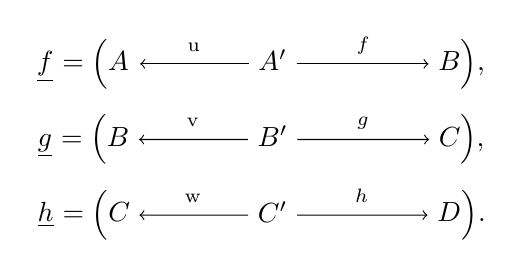
\begin{tikzpicture}[xscale=2.4,yscale=-1.2]
    \def\y{0.8}
    \def\z{0}
    \node (A0_0) at (0, \z*\y) {$\underline{f}_{\CATA}=\Big(A_{\CATA}$};
    \node (A0_1) at (1, \z*\y) {$A'_{\CATA}$};
    \node (A0_2) at (2, \z*\y) {$B_{\CATA}\Big)$,};
    \path (A0_1) edge [->]node [auto,swap] {$\scriptstyle{\operatorname{u}_{\CATA}}$} (A0_0);
    \path (A0_1) edge [->]node [auto] {$\scriptstyle{f_{\CATA}}$} (A0_2);

    \def\z{1}
    \node (B0_0) at (0, \z*\y) {$\underline{g}_{\CATA}=\Big(B_{\CATA}$};
    \node (B0_1) at (1, \z*\y) {$B'_{\CATA}$};
    \node (B0_2) at (2, \z*\y) {$C_{\CATA}\Big)$,};
    \path (B0_1) edge [->]node [auto,swap]{$\scriptstyle{\operatorname{v}_{\CATA}}$} (B0_0);
    \path (B0_1) edge [->]node [auto] {$\scriptstyle{g_{\CATA}}$} (B0_2);

    \def\z{2}
    \node (C0_0) at (0, \z*\y) {$\underline{h}_{\CATA}=\Big(C_{\CATA}$};
    \node (C0_1) at (1, \z*\y) {$C'_{\CATA}$};
    \node (C0_2) at (2, \z*\y) {$D_{\CATA}\Big)$.};
    \path (C0_1) edge [->]node [auto,swap]  {$\scriptstyle{\operatorname{w}_{\CATA}}$} (C0_0);
    \path (C0_1) edge [->]node [auto] {$\scriptstyle{h_{\CATA}}$} (C0_2);
\end{tikzpicture}
\end{equation}

If we want to compute the composition $\underline{h}_{\CATA}\circ(\underline{g}_{\CATA}\circ
\underline{f}_{\CATA})$, then we need to use the fixed choices C$(\SETWA)$
in order to get data as in the upper parts of the following $2$-commutative polygons (starting from
the smaller one), with $\operatorname{u}^1_{\CATA}$ and $\operatorname{u}^2_{\CATA}$ in $\SETWA$ and
$\delta_{\CATA}$ and $\sigma_{\CATA}$ invertible (here $\sigma_{\CATA}$ is defined from
$(g_{\CATA}\circ f^1_{\CATA})\circ\operatorname{u}^2_{\CATA}$ to $\operatorname{w}_{\CATA}\circ
l_{\CATA}$):

\begin{equation}\label{eq-187}
\begin{tikzpicture}[xscale=1.8,yscale=-0.8]

    \def\formaa#1#2#3
    {\begin{scope}[shift={#1}, scale=#2]
    \draw [fill=#3, draw=white, line width=0pt, rounded corners] (3.5, 1.5) -- (5, 6) -- (3, 6) -- (2, 3.5) -- cycle;
    \end{scope}}

    \formaa{(0,0)}{1}{mypaleblue}
    \formaa{(0.95, 1.2)}{0.7}{white}

    %%%
    
    \def\formab#1#2#3
    {\begin{scope}[shift={#1}, scale=#2]
    \draw [fill=#3, draw=white, line width=0pt, rounded corners] (1, 6) -- (2, 3.5) -- (3, 6) -- cycle;
    \end{scope}}

    \formab{(0,0)}{1}{mypalelime}
    \formab{(0.6, 1.5)}{0.7}{white}
   
    %%%
   
    \node (A0_4) at (3.5, 1.5) {$A^2_{\CATA}$};
    \node (A3_2) at (2, 3.5) {$A^1_{\CATA}$};
    \node (A6_1) at (1, 6) {$A'_{\CATA}$};
    \node (A6_2) at (2, 6) {$B_{\CATA}$};
    \node (A6_3) at (3, 6) {$B'_{\CATA}$};
    \node (A6_4) at (4, 6) {$C_{\CATA}$};
    \node (A6_5) at (5, 6) {$C'_{\CATA}$.};
    
    \node (A3_4) at (3.5, 4.5) {$\Rightarrow$};
    \node (A5_2) at (2, 5.2) {$\Rightarrow$};
    
    \node (A4_2) at (2, 4.7) {$\delta_{\CATA}$};
    \node (A2_4) at (3.5, 4) {$\sigma_{\CATA}$};

    \path (A3_2) edge [->]node [auto] {$\scriptstyle{f^1_{\CATA}}$} (A6_3);
    \path (A6_5) edge [->]node [auto] {$\scriptstyle{\operatorname{w}_{\CATA}}$} (A6_4);
    \path (A6_1) edge [->]node [auto,swap] {$\scriptstyle{f_{\CATA}}$} (A6_2);
    \path (A0_4) edge [->]node [auto] {$\scriptstyle{l_{\CATA}}$} (A6_5);
    \path (A0_4) edge [->]node [auto,swap] {$\scriptstyle{\operatorname{u}^2_{\CATA}}$} (A3_2);
    \path (A3_2) edge [->]node [auto,swap] {$\scriptstyle{\operatorname{u}^1_{\CATA}}$} (A6_1);
    \path (A6_3) edge [->]node [auto,swap] {$\scriptstyle{g_{\CATA}}$} (A6_4);
    \path (A6_3) edge [->]node [auto] {$\scriptstyle{\operatorname{v}_{\CATA}}$} (A6_2);
\end{tikzpicture}
\end{equation}

Then according to~\cite[\S~2.2]{Pr} we have

\begin{equation}\label{eq-182}
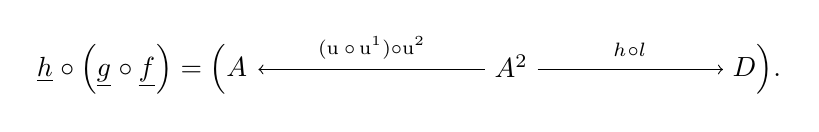
\begin{tikzpicture}[xscale=3.9,yscale=-1.2]
    \node (A0_0) at (-0.2, 0) {$\underline{h}_{\CATA}\circ\left(\underline{g}_{\CATA}
      \circ\underline{f}_{\CATA}\right)=\Big(A_{\CATA}$};
    \node (A0_1) at (1, 0) {$A^2_{\CATA}$};
    \node (A0_2) at (1.8, 0) {$D_{\CATA}\Big)$.};
    \path (A0_1) edge [->]node [auto,swap] {$\scriptstyle{(\operatorname{u}_{\CATA}\circ
      \operatorname{u}^1_{\CATA})\circ\operatorname{u}^2_{\CATA}}$} (A0_0);
    \path (A0_1) edge [->]node [auto] {$\scriptstyle{h_{\CATA}\circ l_{\CATA}}$} (A0_2);
\end{tikzpicture}
\end{equation}

On the other hand, if we want to compute the composition $(\underline{h}_{\CATA}\circ
\underline{g}_{\CATA})\circ\underline{f}_{\CATA}$, then we need to use the fixed choices C$(\SETWA)$
in order to get data as in the upper parts of the following $2$-commutative
polygons (starting from the smaller one), with
$\operatorname{v}^1_{\CATA}$ and $\operatorname{u}^3_{\CATA}$ in $\SETWA$ and $\xi_{\CATA}$ and
$\eta_{\CATA}$ invertible (here $\eta_{\CATA}$ is defined from $f_{\CATA}\circ
\operatorname{u}^3_{\CATA}$ to $(\operatorname{v}_{\CATA}\circ\operatorname{v}^1_{\CATA})\circ
f^2_{\CATA}$):

\begin{equation}\label{eq-188}
\begin{tikzpicture}[xscale=-1.8,yscale=-0.8]

    \def\formaa#1#2#3
    {\begin{scope}[shift={#1}, scale=#2]
    \draw [fill=#3, draw=white, line width=0pt, rounded corners] (3.5, 1.5) -- (5, 6) -- (3, 6) -- (2, 3.5) -- cycle;
    \end{scope}}

    \formaa{(0,0)}{1}{mypalered}
    \formaa{(0.95, 1.2)}{0.7}{white}

    %%%
    
    \def\formab#1#2#3
    {\begin{scope}[shift={#1}, scale=#2]
    \draw [fill=#3, draw=white, line width=0pt, rounded corners] (1, 6) -- (2, 3.5) -- (3, 6) -- cycle;
    \end{scope}}

    \formab{(0,0)}{1}{mypaleyellow}
    \formab{(0.6, 1.5)}{0.7}{white}
    
    %%%

    \node (A0_4) at (3.5, 1.5) {$A^3_{\CATA}$};
    \node (A3_2) at (2, 3.5) {$B^2_{\CATA}$};
    \node (A6_1) at (1, 6) {$C'_{\CATA}$.};
    \node (A6_2) at (2, 6) {$C_{\CATA}$};
    \node (A6_3) at (3, 6) {$B'_{\CATA}$};
    \node (A6_4) at (4, 6) {$B_{\CATA}$};
    \node (A6_5) at (5, 6) {$A'_{\CATA}$};
    
    \node (A3_4) at (3.5, 4.5) {$\Rightarrow$};
    \node (A5_2) at (2, 5.2) {$\Rightarrow$};

    \node (A4_2) at (2, 4.7) {$\xi_{\CATA}$};
    \node (A2_4) at (3.5, 4) {$\eta_{\CATA}$};
    
    \path (A3_2) edge [->]node [auto,swap] {$\scriptstyle{\operatorname{v}^1_{\CATA}}$} (A6_3);
    \path (A6_5) edge [->]node [auto,swap] {$\scriptstyle{f_{\CATA}}$} (A6_4);
    \path (A6_1) edge [->]node [auto] {$\scriptstyle{\operatorname{w}_{\CATA}}$} (A6_2);
    \path (A0_4) edge [->]node [auto,swap] {$\scriptstyle{\operatorname{u}^3_{\CATA}}$} (A6_5);
    \path (A0_4) edge [->]node [auto] {$\scriptstyle{f^2_{\CATA}}$} (A3_2);
    \path (A3_2) edge [->]node [auto] {$\scriptstyle{g^1_{\CATA}}$} (A6_1);
    \path (A6_3) edge [->]node [auto] {$\scriptstyle{\operatorname{v}_{\CATA}}$} (A6_4);
    \path (A6_3) edge [->]node [auto,swap] {$\scriptstyle{g_{\CATA}}$} (A6_2);
\end{tikzpicture}
\end{equation}

Then we have:

\begin{equation}\label{eq-183}
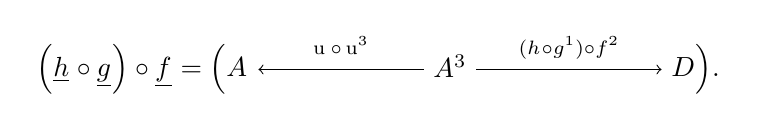
\begin{tikzpicture}[xscale=3.9,yscale=-1.2]
    \node (A0_0) at (0, 0) {$\left(\underline{h}_{\CATA}\circ\underline{g}_{\CATA}\right)\circ
      \underline{f}_{\CATA}=\Big(A_{\CATA}$};
    \node (A0_1) at (1, 0) {$A^3_{\CATA}$};
    \node (A0_2) at (1.8, 0) {$D_{\CATA}\Big)$.};
    \path (A0_1) edge [->]node [auto,swap] {$\scriptstyle{\operatorname{u}_{\CATA}
      \circ\operatorname{u}^3_{\CATA}}$} (A0_0);
    \path (A0_1) edge [->]node [auto]  {$\scriptstyle{(h_{\CATA}\circ
      g^1_{\CATA})\circ f^2_{\CATA}}$} (A0_2);
\end{tikzpicture}
\end{equation}

Then from~\cite[Proposition~0.1]{T3} (for $\CATA$ instead of $\CATC$) we have

\begin{prop}\label{prop-01}
Let us fix any pair $(\CATA,\SETWA)$, satisfying conditions
\emphatic{(BF)}, any triple of morphisms as in \eqref{eq-114}
and let us suppose that choices \emphatic{C}$(\SETWA)$ give data as in the upper parts of diagrams
\eqref{eq-187} and \eqref{eq-188}. Then let us \emph{choose} any set of data as follows:

\begin{enumerate}[\emphatic{(}{F}1\emphatic{)}]
 \item\label{F1} an object $A^4_{\CATA}$, a morphism $\operatorname{u}^4_{\CATA}:A^4_{\CATA}
  \rightarrow A^2_{\CATA}$ in $\SETWA$, a morphism $\operatorname{u}^5_{\CATA}:A^4_{\CATA}\rightarrow
  A^3_{\CATA}$ and an invertible $2$-morphism $\gamma_{\CATA}:\operatorname{u}^1_{\CATA}\circ
  (\operatorname{u}^2_{\CATA}\circ\operatorname{u}^4_{\CATA})
  \Rightarrow\operatorname{u}^3_{\CATA}\circ\operatorname{u}^5_{\CATA}$;
 \item\label{F2} an invertible $2$-morphism $\omega_{\CATA}:f^1_{\CATA}\circ
  (\operatorname{u}^2_{\CATA}\circ\operatorname{u}^4_{\CATA})
  \Longrightarrow\operatorname{v}^1_{\CATA}\circ(f^2_{\CATA}\circ\operatorname{u}^5_{\CATA})$,
  such that $i_{\operatorname{v}_{\CATA}}\ast\omega_{\CATA}$ coincides with the following composition
  \emphatic{(}associators of $\CATA$ omitted\emphatic{)}:
  
  \begin{equation}\label{eq-105}
  \begin{tikzpicture}[xscale=2.8,yscale=-1.8]

    \def\formaa#1#2#3
    {\begin{scope}[shift={#1}, scale=#2]
    \draw [fill=#3, draw=white, line width=0pt, rounded corners] (2, 2) -- (3, 2) -- (2, 3) -- (1, 3) -- cycle;
    \end{scope}}

    \formaa{(0,0)}{1}{mypalered}
    \formaa{(0.6, 0.75)}{0.7}{white}
   
    %%%
   
    \def\formab#1#2#3
    {\begin{scope}[shift={#1}, scale=#2]
    \draw [fill=#3, draw=white, line width=0pt, rounded corners] (0, 2) -- (1, 1) -- (2, 2) -- (1, 3) --cycle;
    \end{scope}}

    \formab{(0,0)}{1}{mypalegray}
    \formab{(0.3, 0.6)}{0.7}{white}
   
    %%%
   
    \def\formac#1#2#3
    {\begin{scope}[shift={#1}, scale=#2]
    \draw [fill=#3, draw=white, line width=0pt, rounded corners] (1, 1) -- (2, 1) -- (3, 2) -- (2, 2) -- cycle;
    \end{scope}}

    \formac{(0,0)}{1}{mypalelime}
    \formac{(0.6,0.45)}{0.7}{white}
    
    %%%
    
    \node (A0_2) at (2, 1) {$B'_{\CATA}$};
    \node (A1_1) at (1, 1) {$A^1_{\CATA}$};
    \node (A1_3) at (3, 2) {$B_{\CATA}$;};
    \node (A2_0) at (0, 2) {$A^4_{\CATA}$};
    \node (A2_2) at (2, 2) {$A'_{\CATA}$};
    \node (A3_1) at (1, 3) {$A^3_{\CATA}$};
    \node (A3_2) at (2, 3) {$B'_{\CATA}$};
    \node (B1_1) at (0.55, 1.45) {$A^2_{\CATA}$};
    
    \node (A1_2) at (2, 1.5) {$\Downarrow\,\delta^{-1}_{\CATA}$};
    \node (A2_1) at (0.9, 2) {$\Downarrow\,\gamma_{\CATA}$};
    \node (A2_3) at (2, 2.5) {$\Downarrow\,\eta_{\CATA}$};

    \path (A2_0) edge [->]node [auto] {$\scriptstyle{\operatorname{u}^4_{\CATA}}$} (B1_1);
    \path (B1_1) edge [->]node [auto] {$\scriptstyle{\operatorname{u}^2_{\CATA}}$} (A1_1);
    
    \path (A1_1) edge [->]node [auto] {$\scriptstyle{f^1_{\CATA}}$} (A0_2);
    \path (A2_2) edge [->]node [auto] {$\scriptstyle{f_{\CATA}}$} (A1_3);
    \path (A3_1) edge [->]node [auto,swap] {$\scriptstyle{\operatorname{v}^1_{\CATA}
      \circ f^2_{\CATA}}$} (A3_2);
    \path (A2_0) edge [->]node [auto,swap] {$\scriptstyle{\operatorname{u}^5_{\CATA}}$} (A3_1);
    \path (A3_1) edge [->]node [auto] {$\scriptstyle{\operatorname{u}^3_{\CATA}}$} (A2_2);
    \path (A1_1) edge [->]node [auto,swap] {$\scriptstyle{\operatorname{u}^1_{\CATA}}$} (A2_2);
    \path (A3_2) edge [->]node [auto,swap] {$\scriptstyle{\operatorname{v}_{\CATA}}$} (A1_3);
    \path (A0_2) edge [->]node [auto] {$\scriptstyle{\operatorname{v}_{\CATA}}$} (A1_3);
  \end{tikzpicture}
  \end{equation}
  
 \item\label{F3} an invertible $2$-morphism $\rho_{\CATA}:\,l_{\CATA}\circ
  \operatorname{u}^4_{\CATA}\Longrightarrow g^1_{\CATA}\circ(f^2_{\CATA}\circ
  \operatorname{u}^5_{\CATA})$, such that $i_{\operatorname{w}_{\CATA}}\ast\rho_{\CATA}$ coincides
  with the following composition \emphatic{(}associators of $\CATA$ omitted\emphatic{)}:
  
  \begin{equation}\label{eq-106}
  \begin{tikzpicture}[xscale=2.8,yscale=-1.8]
  
    \def\formaa#1#2#3
    {\begin{scope}[shift={#1}, scale=#2]
    \draw [fill=#3, draw=white, line width=0pt, rounded corners] (3, 2) -- (4, 2) -- (3, 3) -- (2, 3) -- cycle;
    \end{scope}}

    \formaa{(0,0)}{1}{mypaleyellow}
    \formaa{(0.9,0.75)}{0.7}{white}
   
    %%%
   
    \def\formab#1#2#3
    {\begin{scope}[shift={#1}, scale=#2]
    \draw [fill=#3, draw=white, line width=0pt, rounded corners] (2, 1) -- (3, 1) -- (4, 2) -- (3, 2) -- cycle;
    \end{scope}}
  
    \formab{(0,0)}{1}{mypaleblue}
    \formab{(0.9,0.45)}{0.7}{white}

    %%%
    
    \def\formac#1#2#3
    {\begin{scope}[shift={#1}, scale=#2]
    \draw [fill=#3, draw=white, line width=0pt, rounded corners]  (1, 1) -- (2, 2) -- (0, 2) -- cycle;
    \end{scope}}
 
    %%%
    
    \def\formad#1#2#3
    {\begin{scope}[shift={#1}, scale=#2]
    \draw [fill=#3, draw=white, line width=0pt, rounded corners]  (1, 2) -- (2, 1) -- (3, 2)
      -- (2, 3) -- cycle;
    \end{scope}}
 
    \formad{(0,0)}{1}{mypaleorange}
    \formad{(0.6,0.6)}{0.7}{white}    
    
    %%%
    
    \node (A0_2) at (3, 1) {$C'_{\CATA}$};
    \node (A1_1) at (2, 1) {$A^2_{\CATA}$};
    \node (A2_0) at (1, 2) {$A^4_{\CATA}$};
    \node (A2_3) at (3, 2) {$B'_{\CATA}$};
    \node (A2_4) at (4, 2) {$C_{\CATA}$.};
    \node (A3_1) at (2, 3) {$B^2_{\CATA}$};
    \node (A3_3) at (3, 3) {$C'_{\CATA}$};
    \node (B1_1) at (1.55, 2.55) {$A^3_{\CATA}$};
    
    \node (A3_2) at (1.9, 2) {$\Downarrow\,\omega_{\CATA}$};
    \node (A1_2) at (3, 1.5) {$\Downarrow\,\sigma^{-1}_{\CATA}$};
    \node (A3_4) at (3, 2.6) {$\Downarrow\,\xi_{\CATA}$};
    
    \path (B1_1) edge [->]node [auto,swap] {$\scriptstyle{f^2_{\CATA}}$} (A3_1);
    \path (A2_0) edge [->]node [auto,swap] {$\scriptstyle{\operatorname{u}^5_{\CATA}}$} (B1_1);
    \path (A2_3) edge [->]node [auto] {$\scriptstyle{g_{\CATA}}$} (A2_4);
    \path (A1_1) edge [->]node [auto] {$\scriptstyle{l_{\CATA}}$} (A0_2);
    \path (A3_1) edge [->]node [auto,swap] {$\scriptstyle{g^1_{\CATA}}$} (A3_3);
    \path (A2_0) edge [->]node [auto] {$\scriptstyle{\operatorname{u}^4_{\CATA}}$} (A1_1);
    \path (A1_1) edge [->]node [auto,swap] {$\scriptstyle{f^1_{\CATA}\circ
      \operatorname{u}^2_{\CATA}}$} (A2_3);
    \path (A3_1) edge [->]node [auto] {$\scriptstyle{\operatorname{v}^1_{\CATA}}$} (A2_3);
    \path (A3_3) edge [->]node [auto,swap] {$\scriptstyle{\operatorname{w}_{\CATA}}$} (A2_4);
    \path (A0_2) edge [->]node [auto] {$\scriptstyle{\operatorname{w}_{\CATA}}$} (A2_4);
  \end{tikzpicture}
  \end{equation}
\end{enumerate}

Then the associator $\Theta_{\underline{h}_{\CATA},\underline{g}_{\CATA},
\underline{f}_{\CATA}}^{\CATA,\SETWA}$ from \eqref{eq-182} to \eqref{eq-183}
is given by the class of the following diagram \emphatic{(}associators of $\CATA$ omitted\emphatic{)}:

\begin{equation}\label{eq-101}
\begin{tikzpicture}[xscale=3.0,yscale=-1.5]
    \node (A0_2) at (2, 0) {$A^2_{\CATA}$};
    \node (A2_2) at (2, 2) {$A^4_{\CATA}$};
    \node (A2_4) at (4, 2) {$D_{\CATA}$.};
    \node (A2_0) at (0, 2) {$A_{\CATA}$};
    \node (A4_2) at (2, 4) {$A^3_{\CATA}$};

    \node (A2_3) at (2.8, 2) {$\Downarrow\,i_{h_{\CATA}}\ast\rho_{\CATA}$};
    \node (A2_1) at (1.2, 2) {$\Downarrow\,i_{\operatorname{u}_{\CATA}}\ast\gamma_{\CATA}$};
    
    \path (A4_2) edge [->]node [auto,swap] {$\scriptstyle{(h_{\CATA}\circ
      g^1_{\CATA})\circ f^2_{\CATA}}$} (A2_4);
    \path (A0_2) edge [->]node [auto] {$\scriptstyle{h_{\CATA}\circ l_{\CATA}}$} (A2_4);
    \path (A4_2) edge [->]node [auto]
      {$\scriptstyle{\operatorname{u}_{\CATA}\circ\operatorname{u}^3_{\CATA}}$} (A2_0);
    \path (A0_2) edge [->]node [auto,swap] {$\scriptstyle{(\operatorname{u}_{\CATA}\circ
      \operatorname{u}^1_{\CATA})\circ\operatorname{u}^2_{\CATA}}$} (A2_0);
    \path (A2_2) edge [->]node [auto,swap] {$\scriptstyle{\operatorname{u}^4_{\CATA}}$} (A0_2);
    \path (A2_2) edge [->]node [auto] {$\scriptstyle{\operatorname{u}^5_{\CATA}}$} (A4_2);
\end{tikzpicture}
\end{equation}

Moreover, a set of choices as in \emphatic{(}\hyperref[F1]{F1}\emphatic{)} --
\emphatic{(}\hyperref[F3]{F3}\emphatic{)} always exists
\emphatic{(}see~\cite[Remark~2.1]{T3}\emphatic{)}.
\end{prop}

\section{The definition of $\functor{N}$}
We recall that in the present paper we have fixed any pseudofunctor $\functor{F}:\CATA\rightarrow\CATB$ that maps
any morphism of $\SETWA$ to some morphism of $\SETWBsat$.\\

For each object $A_{\CATA}$, we define $\functor{N}_0(A_{\CATA}):=\functor{F}_0
(A_{\CATA})$; for each morphism $\underline{f}_{\CATA}:=(A'_{\CATA},\operatorname{w}_{\CATA},f_{\CATA}):
A_{\CATA}\rightarrow B_{\CATA}$ in $\CATA\left[\SETWAinv\right]$, we set

\[\functor{N}_1
(\underline{f}_{\CATA}):=\Big(\functor{F}_0(A'_{\CATA}),\functor{F}_1(\operatorname{w}_{\CATA}),
\functor{F}_1(f_{\CATA})\Big).\]

Given any pair of morphisms $(A^m_{\CATA},\operatorname{w}^m_{\CATA},f^m_{\CATA}):A_{\CATA}\rightarrow B_{\CATA}$ in
$\CATA\left[\SETWAinv\right]$ for $m=1,2$ and any $2$-morphism 

\[\Big[A^3_{\CATA},\operatorname{v}^1_{\CATA},\operatorname{v}^2_{\CATA},\alpha_{\CATA},
\beta_{\CATA}\Big]:\Big(A^1_{\CATA},\operatorname{w}^1_{\CATA},f^1_{\CATA}\Big)\Longrightarrow
\Big(A^2_{\CATA},\operatorname{w}^2_{\CATA},f^2_{\CATA}\Big)\]
%
in $\CATA\left[\SETWAinv\right]$, we set

\begin{gather}
\label{eq-120} \functor{N}_2\Big(\Big[A^3_{\CATA},\operatorname{v}^1_{\CATA},
 \operatorname{v}^2_{\CATA},\alpha_{\CATA},\beta_{\CATA}\Big]\Big):=\Big[\functor{F}_0
 (A^3_{\CATA}),\functor{F}_1(\operatorname{v}^1_{\CATA}),\functor{F}_1(\operatorname{v}^2_{\CATA}),\\
%%%
\nonumber \psi^{\functor{F}}_{\operatorname{w}^2_{\CATA},\operatorname{v}^2_{\CATA}}\odot\functor{F}_2
 (\alpha_{\CATA})\odot\Big(\psi^{\functor{F}}_{\operatorname{w}^1_{\CATA},
 \operatorname{v}^1_{\CATA}}\Big)^{-1},\psi^{\functor{F}}_{f^2_{\CATA},\operatorname{v}^2_{\CATA}}
 \odot\functor{F}_2(\beta_{\CATA})\odot
 \Big(\psi^{\functor{F}}_{f^1_{\CATA},\operatorname{v}^1_{\CATA}}\Big)^{-1}\Big].
\end{gather}

First of all, we have to show that $\functor{N}_2$ is well-defined. So let us suppose that
we have

\[\Big[A^3_{\CATA},\operatorname{v}^1_{\CATA},\operatorname{v}^2_{\CATA},\alpha_{\CATA},
\beta_{\CATA}\Big]=\Big[A^{\prime 3}_{\CATA},\operatorname{v}^{\prime 1}_{\CATA},
\operatorname{v}^{\prime 2}_{\CATA},\alpha'_{\CATA},\beta'_{\CATA}\Big].\]

By definition of $2$-morphisms in $\CATA\left[\SETWAinv\right]$ (see~\cite[\S~2.3]{Pr}),
this implies that
there is a set of data $(A^4_{\CATA},\operatorname{z}_{\CATA},\operatorname{z}'_{\CATA},
\rho_{\CATA},\varepsilon_{\CATA})$ in $\CATA$ as in the following diagram

\[
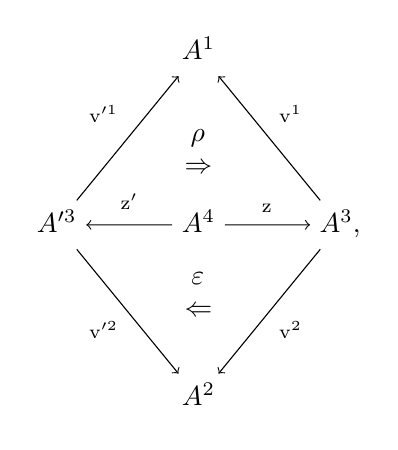
\begin{tikzpicture}[xscale=1.8,yscale=-1.1]
    \node (A4_4) at (4, 4) {$A^2_{\CATA}$};
    \node (A0_4) at (4, 0) {$A^1_{\CATA}$};
    \node (A2_2) at (3, 2) {$A^{\prime 3}_{\CATA}$};
    \node (A2_4) at (4, 2) {$A^4_{\CATA}$};
    \node (A2_6) at (5, 2) {$A^3_{\CATA}$,};
    
    \node (A3_4) at (4, 3) {$\Leftarrow$};
    \node (A1_4) at (4, 1.35) {$\Rightarrow$};
    
    \node (B3_4) at (4, 2.65) {$\varepsilon_{\CATA}$};
    \node (B1_4) at (4, 1) {$\rho_{\CATA}$};
    
    \path (A2_2) edge [->]node [auto,swap]
      {$\scriptstyle{\operatorname{v}^{\prime 2}_{\CATA}}$} (A4_4);
    \path (A2_4) edge [->]node [auto] {$\scriptstyle{\operatorname{z}_{\CATA}}$} (A2_6);
    \path (A2_6) edge [->]node [auto] {$\scriptstyle{\operatorname{v}^2_{\CATA}}$} (A4_4);
    \path (A2_2) edge [->]node [auto] {$\scriptstyle{\operatorname{v}^{\prime 1}_{\CATA}}$} (A0_4);
    \path (A2_4) edge [->]node [auto,swap] {$\scriptstyle{\operatorname{z}'_{\CATA}}$} (A2_2);
    \path (A2_6) edge [->]node [auto,swap] {$\scriptstyle{\operatorname{v}^1_{\CATA}}$} (A0_4);
\end{tikzpicture}
\]
%
such that $(\operatorname{w}^1_{\CATA}\circ\operatorname{v}^1_{\CATA})\circ\operatorname{z}_{\CATA}$
belongs to $\SETWA$, $\rho_{\CATA}$ and $\varepsilon_{\CATA}$ are both invertible,

\begin{gather*}
\Big(i_{\operatorname{w}^2_{\CATA}}\ast\varepsilon_{\CATA}\Big)\odot
 \left(\thetaa{\operatorname{w}^2_{\CATA}}
 {\operatorname{v}^2_{\CATA}}{\operatorname{z}_{\CATA}}\right)^{-1}\odot\Big(\alpha_{\CATA}\ast
 i_{\operatorname{z}_{\CATA}}\Big)\odot\thetaa{\operatorname{w}^1_{\CATA}}
 {\operatorname{v}^1_{\CATA}}{\operatorname{z}_{\CATA}}\odot\Big(i_{\operatorname{w}^1_{\CATA}}\ast
 \rho_{\CATA}\Big)= \\
%%%
=\left(\thetaa{\operatorname{w}^2_{\CATA}}{\operatorname{v}^{\prime 2}_{\CATA}}
 {\operatorname{z}'_{\CATA}}\right)^{-1}
 \odot\Big(\alpha'_{\CATA}\ast i_{\operatorname{z}'_{\CATA}}\Big)\odot
 \thetaa{\operatorname{w}^1_{\CATA}}{\operatorname{v}^{\prime 1}_{\CATA}}{\operatorname{z}'_{\CATA}}
\end{gather*}
%
and

\begin{gather*}
\Big(i_{f^2_{\CATA}}\ast\varepsilon_{\CATA}\Big)\odot\left(\thetaa{f^2_{\CATA}}{\operatorname{v}^2_{\CATA}}
 {\operatorname{z}_{\CATA}}\right)^{-1}\odot\Big(\beta_{\CATA}\ast i_{\operatorname{z}_{\CATA}}\Big)\odot
 \thetaa{f^1_{\CATA}}{\operatorname{v}^1_{\CATA}}{\operatorname{z}_{\CATA}}\odot\Big(i_{f^1_{\CATA}}
 \ast\rho_{\CATA}\Big)= \\
%%%
=\left(\thetaa{f^2_{\CATA}}{\operatorname{v}^{\prime 2}_{\CATA}}{\operatorname{z}'_{\CATA}}\right)^{-1}\odot\Big(
 \beta'_{\CATA}\ast i_{\operatorname{z}'_{\CATA}}\Big)\odot\thetaa{f^1_{\CATA}}
 {\operatorname{v}^{\prime 1}_{\CATA}}{\operatorname{z}'_{\CATA}}.
\end{gather*}

Then the following set of data proves that $\functor{N}$ is well-defined on $2$-morphisms;
the $2$-morphisms without a name below are all $2$-morphisms of the form $\psi^{\functor{F}}_{-,-}$
(see \eqref{eq-185}) or inverses of such $2$-morphisms:

\[
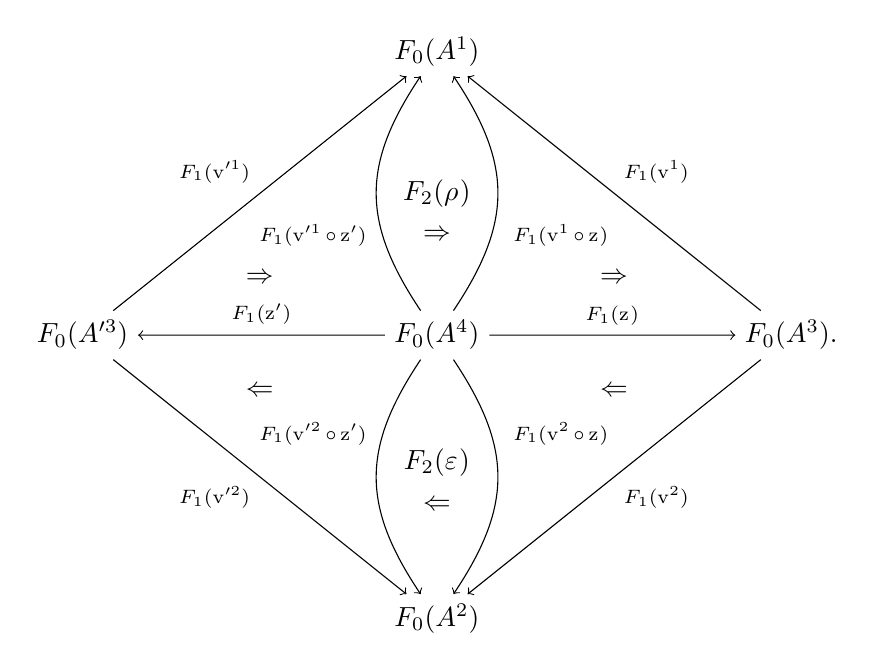
\begin{tikzpicture}[xscale=4.5,yscale=-1.8]
    \node (A0_4) at (4, 0) {$\functor{F}_0(A^1_{\CATA})$};
    \node (A2_2) at (3, 2) {$\functor{F}_0(A^{\prime 3}_{\CATA})$};
    \node (A2_4) at (4, 2) {$\functor{F}_0(A^4_{\CATA})$};
    \node (A2_6) at (5, 2) {$\functor{F}_0(A^3_{\CATA})$.};
    \node (A4_4) at (4, 4) {$\functor{F}_0(A^2_{\CATA})$};
    \node (C1_1) at (3.65, 1.3)  {$\scriptstyle{\functor{F}_1
     (\operatorname{v}^{\prime 1}_{\CATA}\circ\operatorname{z}'_{\CATA})}$};
    \node (C2_2) at (3.65, 2.7)  {$\scriptstyle{\functor{F}_1
     (\operatorname{v}^{\prime 2}_{\CATA}\circ\operatorname{z}'_{\CATA})}$};
    \node (C3_3) at (4.35, 1.3) {$\scriptstyle{\functor{F}_1
     (\operatorname{v}^1_{\CATA}\circ\operatorname{z}_{\CATA})}$};
    \node (C4_4) at (4.35, 2.7){$\scriptstyle{\functor{F}_1
     (\operatorname{v}^2_{\CATA}\circ\operatorname{z}_{\CATA})}$};

    \node (B1_4) at (4, 1) {$\functor{F}_2(\rho_{\CATA})$};
    \node (B3_4) at (4, 2.9) {$\functor{F}_2(\varepsilon_{\CATA})$};
    \node (A1_4) at (4, 1.3) {$\Rightarrow$};
    \node (D1_1) at (3.5, 1.6) {$\Rightarrow$};
    \node (D2_2) at (3.5, 2.4) {$\Leftarrow$};
    \node (D3_3) at (4.5, 1.6) {$\Rightarrow$};
    \node (D4_4) at (4.5, 2.4) {$\Leftarrow$};
    \node (A3_4) at (4, 3.2) {$\Leftarrow$};
     
    \path (A2_2) edge [->]node [auto,swap]
      {$\scriptstyle{\functor{F}_1(\operatorname{v}^{\prime 2}_{\CATA}})$} (A4_4);
    \path (A2_4) edge [->]node [auto] {$\scriptstyle{\functor{F}_1
      (\operatorname{z}_{\CATA})}$} (A2_6);
    \path (A2_6) edge [->]node [auto] {$\scriptstyle{\functor{F}_1
      (\operatorname{v}^2_{\CATA})}$} (A4_4);
    \path (A2_2) edge [->]node [auto] {$\scriptstyle{\functor{F}_1
      (\operatorname{v}^{\prime 1}_{\CATA})}$} (A0_4);
    \path (A2_4) edge [->]node [auto,swap] {$\scriptstyle{\functor{F}_1
      (\operatorname{z}'_{\CATA})}$} (A2_2);
    \path (A2_6) edge [->]node [auto,swap] {$\scriptstyle{\functor{F}_1
      (\operatorname{v}^1_{\CATA})}$} (A0_4);
   \path (A2_4) edge [->,bend right=15]node [auto] {} (A0_4);
   \path (A2_4) edge [->,bend left=15]node [auto,swap] {} (A0_4);
   \path (A2_4) edge [->,bend left=15]node [auto,swap] {} (A4_4);
   \path (A2_4) edge [->,bend right=15]node [auto] {} (A4_4);
\end{tikzpicture}
\]

The aim of this paper is to prove that the triple $(\functor{N}_0,
\functor{N}_1,\functor{N}_2)$ induces a pseudofunctor
$\functor{N}:\CATA\left[\SETWAinv\right]\rightarrow\CATB\left[\SETWBsatinv\right]$.
In order to do that, first of all we have to define the unitors for
$\functor{N}$. So let us fix any object $A_{\CATA}$; the identity for it
in $\CATA\left[\SETWAinv\right]$ is the triple $(A_{\CATA},\id_{A_{\CATA}},\id_{A_{\CATA}})$
and analogously for the identity of $\functor{N}_0(A_{\CATA})=\functor{F}_0
(A_{\CATA})$ in $\CATB\left[\SETWBsatinv\right]$.
Then we define the unitor of $\functor{N}$ relative to $A_{\CATA}$

\begin{gather*}
\Sigma_{A_{\CATA}}^{\functor{N}}:\,\functor{N}_1(\id_{A_{\CATA}})=\Big(\functor{F}_0
 (A_{\CATA}),\functor{F}_1(\id_{A_{\CATA}}),\functor{F}_1(\id_{A_{\CATA}})\Big)
 \Longrightarrow \\
%%%
\Longrightarrow\Big(\functor{F}_0(A_{\CATA}),\id_{\functor{F}_0(A_{\CATA})},\id_{\functor{F}_0
 (A_{\CATA})}\Big)=\id_{\functor{N}_0(A_{\CATA})}
\end{gather*}
%
as the class of the following data; here $\sigma_{\bullet}^{\functor{F}}$ is as in \eqref{eq-186}
and the unitors $\pi_{\bullet}$ are the unitors in $\CATB$:

\[
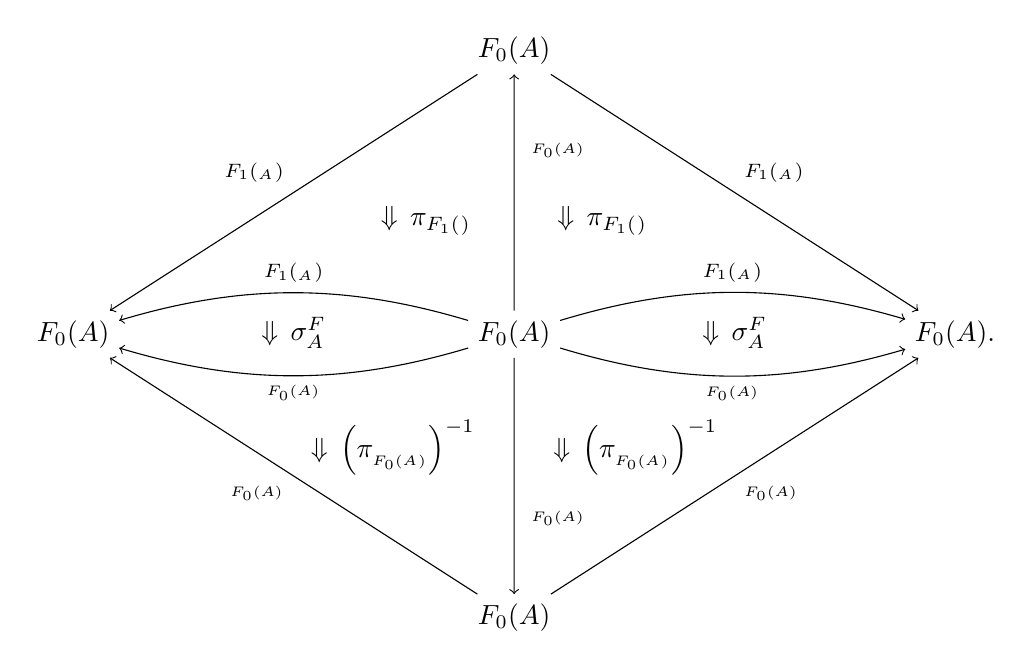
\begin{tikzpicture}[xscale=2.8,yscale=-1.8]
    \node (A0_2) at (2, 0) {$\functor{F}_0(A)$};
    \node (A2_2) at (2, 2) {$\functor{F}_0(A)$};
    \node (A2_0) at (0, 2) {$\functor{F}_0(A)$};
    \node (C1_1) at (2.2, 0.7) {$\scriptstyle{\id_{\functor{F}_0(A)}}$};
    \node (C2_2) at (2.2, 3.3) {$\scriptstyle{\id_{\functor{F}_0(A)}}$};
    \node (A2_4) at (4, 2) {$\functor{F}_0(A)$.};
    \node (A4_2) at (2, 4) {$\functor{F}_0(A)$};

    \node (A2_3) at (3, 2) {$\Downarrow\,\sigma_{A_{\CATA}}^{\functor{F}}$};
    \node (A2_1) at (1, 2) {$\Downarrow\,\sigma_{A_{\CATA}}^{\functor{F}}$};
    \node (B2_1) at (1.6, 1.2) {$\Downarrow\,\pi_{\functor{F}_1(\id_{\CATA})}$};
    \node (B2_1) at (1.45, 2.8) {$\Downarrow\,
      \left(\pi_{\id_{\functor{F}_0(A_{\CATA})}}\right)^{-1}$};
    \node (B2_3) at (2.4, 1.2) {$\Downarrow\,\pi_{\functor{F}_1(\id_{\CATA})}$};
    \node (B2_3) at (2.55, 2.8) {$\Downarrow\,
      \left(\pi_{\id_{\functor{F}_0(A_{\CATA})}}\right)^{-1}$};
    
    \path (A4_2) edge [->]node [auto,swap] {$\scriptstyle{\id_{\functor{F}_0(A)}}$} (A2_4);
    \path (A0_2) edge [->]node [auto] {$\scriptstyle{\functor{F}_1(\id_{A_{\CATA}})}$} (A2_4);
    \path (A2_2) edge [->]node [auto] {} (A0_2);
    \path (A2_2) edge [->]node [auto,swap] {} (A4_2);
    \path (A2_2) edge [->,bend left=25]node [auto,swap]
      {$\scriptstyle{\functor{F}_1(\id_{A_{\CATA}})}$} (A2_0);
    \path (A2_2) edge [->,bend right=25]node [auto]
      {$\scriptstyle{\id_{\functor{F}_0(A)}}$} (A2_0);
    \path (A2_2) edge [->,bend right=25]node [auto]
      {$\scriptstyle{\functor{F}_1(\id_{A_{\CATA}})}$} (A2_4);
    \path (A2_2) edge [->,bend left=25]node [auto,swap]
      {$\scriptstyle{\id_{\functor{F}_0(A)}}$} (A2_4);
    \path (A4_2) edge [->]node [auto] {$\scriptstyle{\id_{\functor{F}_0(A)}}$} (A2_0);
    \path (A0_2) edge [->]node [auto,swap] {$\scriptstyle{\functor{F}_1(\id_{A_{\CATA}})}$} (A2_0);
\end{tikzpicture}
\]

We omit the easy proof that actually this gives a set of unitors for $\functor{N}$.\\

Now we want to compute a set of associators for $\functor{N}$. So let us fix
any pair of composable $2$-morphisms from $A_{\CATA}$ to $B_{\CATA}$ and from $B_{\CATA}$ to
$C_{\CATA}$ in $\CATA\left[\SETWAinv\right]$ as follows

\[
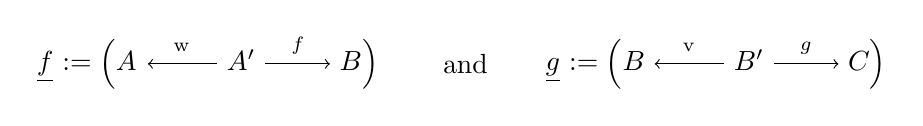
\begin{tikzpicture}[xscale=1.5,yscale=-1.2]
    \node (A0_0) at (-0.3, 0) {$\underline{f}_{\CATA}:=\Big(A_{\CATA}$};
    \node (A0_1) at (1, 0) {$A'_{\CATA}$};
    \node (A0_2) at (2, 0) {$B_{\CATA}\Big)$};
    \node (A0_3) at (2.9, 0) {$\textrm{and}$};
    \path (A0_1) edge [->]node [auto,swap] {$\scriptstyle{\operatorname{w}_{\CATA}}$} (A0_0);
    \path (A0_1) edge [->]node [auto] {$\scriptstyle{f_{\CATA}}$} (A0_2);
    
    \node (A0_4) at (4, 0) {$\underline{g}_{\CATA}:=\Big(B_{\CATA}$};
    \node (A0_5) at (5.3, 0) {$B'_{\CATA}$};
    \node (A0_6) at (6.3, 0) {$C_{\CATA}\Big)$};
    \path (A0_5) edge [->]node [auto,swap] {$\scriptstyle{\operatorname{v}_{\CATA}}$} (A0_4);
    \path (A0_5) edge [->]node [auto] {$\scriptstyle{g_{\CATA}}$} (A0_6);
\end{tikzpicture}
\]
%
(with both $\operatorname{w}_{\CATA}$ and $\operatorname{v}_{\CATA}$ in $\SETWA$) and let us suppose
that choices C$(\SETWA)$ give data as in the upper part of the
following diagram, with $\operatorname{v}'_{\CATA}$ in $\SETWA$ and $\rho_{\CATA}$ invertible:

\[
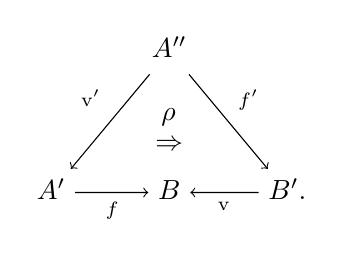
\begin{tikzpicture}[xscale=1.5,yscale=-1.2]
    \node (A0_1) at (1, 0.5) {$A''_{\CATA}$};
    \node (A1_0) at (0, 2) {$A'_{\CATA}$};
    \node (A1_1) at (1, 1.2) {$\rho_{\CATA}$};
    \node (B1_1) at (1, 1.5) {$\Rightarrow$};
    \node (A1_2) at (2, 2) {$B'_{\CATA}$.};
    \node (A2_1) at (1, 2) {$B_{\CATA}$};
    
    \path (A1_2) edge [->]node [auto] {$\scriptstyle{\operatorname{v}_{\CATA}}$} (A2_1);
    \path (A0_1) edge [->]node [auto] {$\scriptstyle{f'_{\CATA}}$} (A1_2);
    \path (A1_0) edge [->]node [auto,swap] {$\scriptstyle{f_{\CATA}}$} (A2_1);
    \path (A0_1) edge [->]node [auto,swap] {$\scriptstyle{\operatorname{v}'_{\CATA}}$} (A1_0);
\end{tikzpicture}
\]

Moreover, let us suppose that choices C$(\SETWBsat)$ give data as in
the upper part of the following diagram, with $\operatorname{v}'_{\CATB}$ in $\SETWBsat$ and
$\rho_{\CATB}$ invertible:

\[
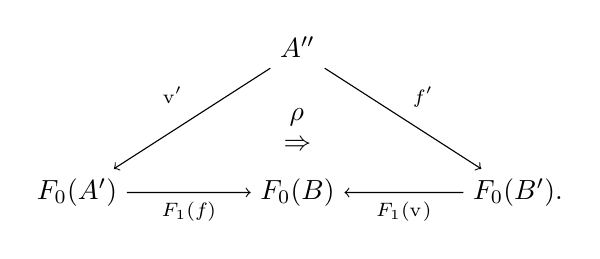
\begin{tikzpicture}[xscale=2.8,yscale=-1.2]
    \node (A0_1) at (1, 0.5) {$A''_{\CATB}$};
    \node (A1_0) at (0, 2) {$\functor{F}_0(A'_{\CATA})$};
    \node (A1_1) at (1, 1.2) {$\rho_{\CATB}$};
    \node (B1_1) at (1, 1.5) {$\Rightarrow$};
    \node (A1_2) at (2, 2) {$\functor{F}_0(B'_{\CATA})$.};
    \node (A2_1) at (1, 2) {$\functor{F}_0(B_{\CATA})$};
    
    \path (A1_2) edge [->]node [auto]
      {$\scriptstyle{\functor{F}_1(\operatorname{v}_{\CATA})}$} (A2_1);
    \path (A0_1) edge [->]node [auto] {$\scriptstyle{f'_{\CATB}}$} (A1_2);
    \path (A1_0) edge [->]node [auto,swap] {$\scriptstyle{\functor{F}_1(f_{\CATA})}$} (A2_1);
    \path (A0_1) edge [->]node [auto,swap] {$\scriptstyle{\operatorname{v}'_{\CATB}}$} (A1_0);
\end{tikzpicture}
\]

Then we have

\[
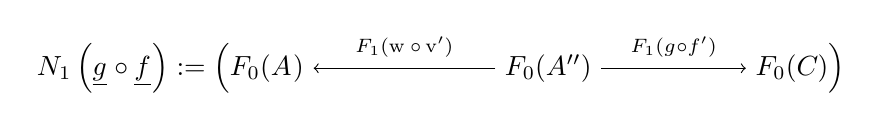
\begin{tikzpicture}[xscale=3.2,yscale=-1.2]
    \node (A0_0) at (-0.5, 0) {$\functor{N}_1\left(\underline{g}_{\CATA}\circ
      \underline{f}_{\CATA}\right):=\Big(\functor{F}_0(A_{\CATA})$};
    \node (A0_1) at (1, 0) {$\functor{F}_0(A''_{\CATA})$};
    \node (A0_2) at (2, 0) {$\functor{F}_0(C_{\CATA})\Big)$};
    \path (A0_1) edge [->]node [auto,swap] {$\scriptstyle{\functor{F}_1(\operatorname{w}_{\CATA}
      \circ\operatorname{v}'_{\CATA})}$} (A0_0);
    \path (A0_1) edge [->]node [auto]
     {$\scriptstyle{\functor{F}_1(g_{\CATA}\circ f'_{\CATA})}$} (A0_2);
\end{tikzpicture}
\]
%
and

\[
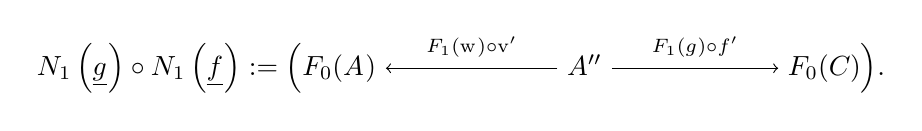
\begin{tikzpicture}[xscale=3.2,yscale=-1.2]
    \node (A0_0) at (-0.5, 0) {$\functor{N}_1\left(\underline{g}_{\CATA}\right)\circ
      \functor{N}_1\left(\underline{f}_{\CATA}\right):=\Big(\functor{F}_0(A_{\CATA})$};
    \node (A0_1) at (1, 0) {$A''_{\CATB}$};
    \node (A0_2) at (2, 0) {$\functor{F}_0(C_{\CATA})\Big)$.};
    \path (A0_1) edge [->]node [auto,swap] {$\scriptstyle{\functor{F}_1(\operatorname{w}_{\CATA})
      \circ\operatorname{v}'_{\CATB}}$} (A0_0);
    \path (A0_1) edge [->]node [auto]
     {$\scriptstyle{\functor{F}_1(g_{\CATA})\circ f'_{\CATB}}$} (A0_2);
\end{tikzpicture}
\]

Using (BF3) for $(\CATB,\SETWBsat)$, there are data as in the upper part of the following diagram, with
$\operatorname{z}^1_{\CATB}$ in $\SETWBsat$ and $\nu_{\CATB}$ invertible:

\[
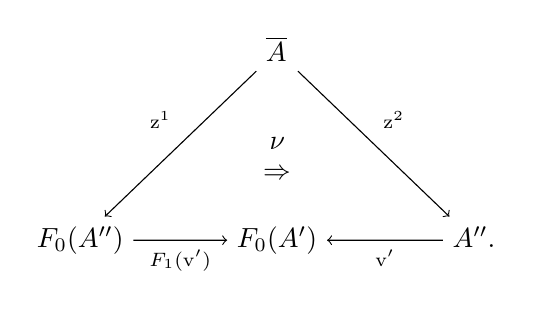
\begin{tikzpicture}[xscale=2.5,yscale=-1.2]
    \node (A0_1) at (0, 2) {$\functor{F}_0(A''_{\CATA})$};
    \node (A1_0) at (1, 0) {$\overline{A}_{\CATB}$};
    \node (A1_1) at (1, 1) {$\nu_{\CATB}$};
    \node (B1_1) at (1, 1.3) {$\Rightarrow$};
    \node (A1_2) at (1, 2) {$\functor{F}_0(A'_{\CATA})$};
    \node (A2_1) at (2, 2) {$A''_{\CATB}$.};
    
    \path (A1_0) edge [->]node [auto,swap] {$\scriptstyle{\operatorname{z}^1_{\CATB}}$} (A0_1);
    \path (A1_0) edge [->]node [auto] {$\scriptstyle{\operatorname{z}^2_{\CATB}}$} (A2_1);
    \path (A0_1) edge [->]node [auto,swap]
      {$\scriptstyle{\functor{F}_1(\operatorname{v}'_{\CATA})}$} (A1_2);
    \path (A2_1) edge [->]node [auto] {$\scriptstyle{\operatorname{v}'_{\CATB}}$} (A1_2);
\end{tikzpicture}
\]

Moreover, using (BF4a) and (BF4b)
for $(\CATB,\SETWBsat)$, there is an object
$\widetilde{A}_{\CATB}$, a morphism $\operatorname{t}_{\CATB}:\widetilde{A}_{\CATB}\rightarrow
\overline{A}_{\CATB}$ in $\SETWBsat$ and an invertible $2$-morphism

\[\beta_{\CATB}:\,(\functor{F}_1(f'_{\CATA})\circ\operatorname{z}^1_{\CATB})\circ
\operatorname{t}_{\CATB}\Longrightarrow(f'_{\CATB}\circ\operatorname{z}^2_{\CATB})\circ
\operatorname{t}_{\CATB},\]
%
such that $i_{\functor{F}_1(\operatorname{v}_{\CATA})}\ast\beta_{\CATB}$ is equal to the following
composition (where all the $2$-morphisms $\theta_{\bullet}$ are associators or
inverses of associators in $\CATB$):

\[
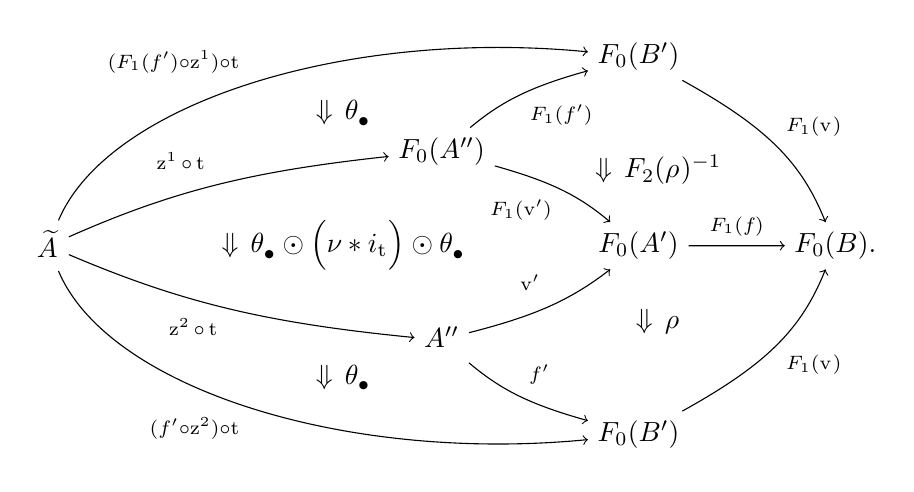
\begin{tikzpicture}[xscale=2.5,yscale=-1.2]
    \node (A0_3) at (3, 0) {$\functor{F}_0(B'_{\CATA})$};
    \node (A1_2) at (2, 1) {$\functor{F}_0(A''_{\CATA})$};
    \node (A2_0) at (0, 2) {$\widetilde{A}_{\CATB}$};
    \node (A2_3) at (3, 2) {$\functor{F}_0(A'_{\CATA})$};
    \node (A2_4) at (4, 2) {$\functor{F}_0(B_{\CATA})$.};
    \node (A3_2) at (2, 3) {$A''_{\CATB}$};
    \node (A4_3) at (3, 4) {$\functor{F}_0(B'_{\CATA})$};

    \node (A3_3) at (3.1, 2.8) {$\Downarrow\,\rho_{\CATB}$};
    \node (B1_1) at (1.5, 0.6) {$\Downarrow\,\theta_{\bullet}^{\CATB}$};
    \node (B2_2) at (1.5, 3.4) {$\Downarrow\,\theta_{\bullet}^{\CATB}$};
    \node (A2_2) at (1.5, 2) {$\Downarrow\,\theta_{\bullet}^{\CATB}\odot\Big(\nu_{\CATB}\ast
      i_{\operatorname{t}_{\CATB}}\Big)\odot\theta_{\bullet}^{\CATB}$};
    \node (A1_3) at (3.1, 1.2) {$\Downarrow\,\functor{F}_2(\rho_{\CATA})^{-1}$};

    \path (A1_2) edge [->,bend right=15]node [auto,swap]
      {$\scriptstyle{\functor{F}_1(f'_{\CATA})}$} (A0_3);
    \path (A1_2) edge [->,bend right=15]node [auto,swap]
      {$\scriptstyle{\functor{F}_1(\operatorname{v}'_{\CATA})}$} (A2_3);
    \path (A0_3) edge [->,bend right=15]node [auto]
      {$\scriptstyle{\functor{F}_1(\operatorname{v}_{\CATA})}$} (A2_4);
    \path (A3_2) edge [->,bend left=15]node [auto]
      {$\scriptstyle{\operatorname{v}'_{\CATB}}$} (A2_3);
    \path (A2_3) edge [->]node [auto] {$\scriptstyle{\functor{F}_1(f_{\CATA})}$} (A2_4);
    \path (A3_2) edge [->,bend left=15]node [auto] {$\scriptstyle{f'_{\CATB}}$} (A4_3);
    \path (A2_0) edge [->,bend right=15]node [auto]
      {$\scriptstyle{\operatorname{z}^1_{\CATB}\circ\operatorname{t}_{\CATB}}$} (A1_2);
    \path (A2_0) edge [->,bend right=45]node [auto] {$\scriptstyle{(\functor{F}_1(f'_{\CATA})
      \circ\operatorname{z}^1_{\CATB})\circ\operatorname{t}_{\CATB}}$} (A0_3);
   \path (A4_3) edge [->,bend left=15]node [auto,swap]
      {$\scriptstyle{\functor{F}_1(\operatorname{v}_{\CATA})}$} (A2_4);
    \path (A2_0) edge [->,bend left=15]node [auto,swap]
      {$\scriptstyle{\operatorname{z}^2_{\CATB}\circ\operatorname{t}_{\CATB}}$} (A3_2);
    \path (A2_0) edge [->,bend left=45]node [auto,swap] {$\scriptstyle{(f'_{\CATB}
      \circ\operatorname{z}^2_{\CATB})\circ\operatorname{t}_{\CATB}}$} (A4_3);
\end{tikzpicture}
\]

Then we define the associator

\begin{gather}
\nonumber \Psi^{\functor{N}}_{\underline{g}_{\CATA},\underline{f}_{\CATA}}:\,\Big(\functor{F}_0
 (A''_{\CATA}),\functor{F}_1(\operatorname{w}_{\CATA}\circ\operatorname{v}'_{\CATA}),\functor{F}_1
 (g_{\CATA}\circ f'_{\CATA})\Big)\Longrightarrow \\
\label{eq-190} \Longrightarrow\Big(A''_{\CATB},\functor{F}_1
 (\operatorname{w}_{\CATA})\circ\operatorname{v}'_{\CATB},\functor{F}_1(g_{\CATA})\circ f'_{\CATB}\Big)
\end{gather}
%
as the class of the following diagram, where for simplicity we have omitted all the necessary
associators $\theta_{\bullet}$ for $\CATB$:

\begin{equation}\label{eq-102}
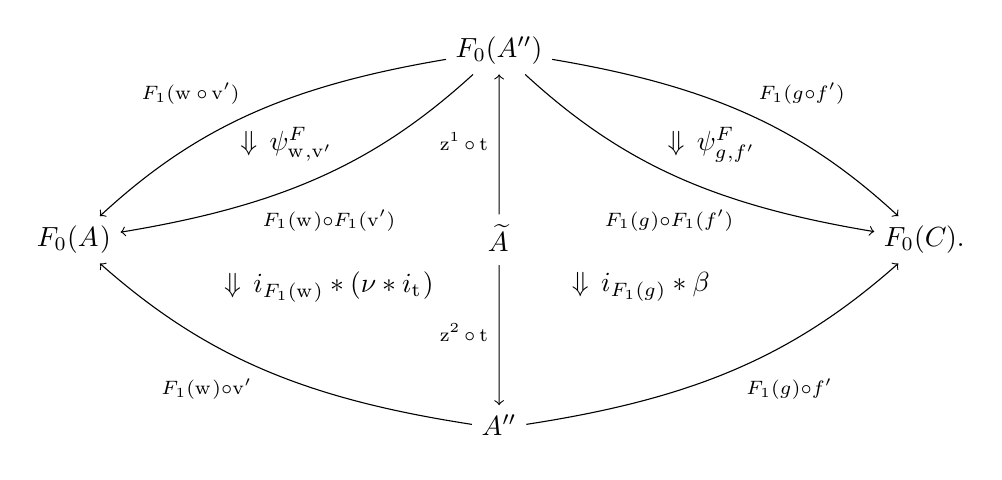
\begin{tikzpicture}[xscale=1.8,yscale=-1.2]
    \node (A0_3) at (3, 0) {$\functor{F}_0(A''_{\CATA})$};
    \node (A2_0) at (0, 2) {$\functor{F}_0(A_{\CATA})$};
    \node (A2_3) at (3, 2) {$\widetilde{A}_{\CATB}$};
    \node (A2_6) at (6, 2) {$\functor{F}_0(C_{\CATA})$.};
    \node (A4_3) at (3, 4) {$A''_{\CATB}$};
    \node (B1_1) at (1.8, 1.8) {$\scriptstyle{\functor{F}_1(\operatorname{w}_{\CATA})
      \circ\functor{F}_1(\operatorname{v}'_{\CATA})}$};
    \node (B2_2) at (4.2, 1.8) {$\scriptstyle{\functor{F}_1(g_{\CATA})
      \circ\functor{F}_1(f'_{\CATA})}$};

    \node (A2_4) at (4, 2.5) {$\Downarrow\,i_{\functor{F}_1(g_{\CATA})}\ast\beta_{\CATB}$};
    \node (A0_2) at (1.5, 1) {$\Downarrow\,\psi_{\operatorname{w}_{\CATA},
      \operatorname{v}'_{\CATA}}^{\functor{F}}$};
    \node (A0_4) at (4.5, 1) {$\Downarrow\,\psi_{g_{\CATA},f'_{\CATA}}^{\functor{F}}$};
    \node (A1_2) at (1.8, 2.5) {$\Downarrow\,i_{\functor{F}_1
      (\operatorname{w}_{\CATA})}\ast(\nu_{\CATB}\ast i_{\operatorname{t}_{\CATB}})$};

    \path (A2_3) edge [->]node [auto]
      {$\scriptstyle{\operatorname{z}^1_{\CATB}\circ\operatorname{t}_{\CATB}}$} (A0_3);
    \path (A2_3) edge [->]node [auto,swap]
      {$\scriptstyle{\operatorname{z}^2_{\CATB}\circ\operatorname{t}_{\CATB}}$} (A4_3);
    \path (A0_3) edge [->,bend left=20]node [auto,swap]
      {$\scriptstyle{\functor{F}_1(\operatorname{w}_{\CATA}\circ\operatorname{v}'_{\CATA})}$} (A2_0);
    \path (A0_3) edge [->,bend right=20]node [auto] {} (A2_0);
    \path (A0_3) edge [->,bend right=20]node [auto] {$\scriptstyle{\functor{F}_1(g_{\CATA}
      \circ f'_{\CATA})}$} (A2_6);
    \path (A0_3) edge [->,bend left=20]node [auto,swap] {} (A2_6);
    \path (A4_3) edge [->,bend left=20]node [auto,swap]
      {$\scriptstyle{\functor{F}_1(g_{\CATA})\circ f'_{\CATB}}$} (A2_6);
    \path (A4_3) edge [->,bend right=20]node [auto]
      {$\scriptstyle{\functor{F}_1(\operatorname{w}_{\CATA})\circ\operatorname{v}'_{\CATB}}$} (A2_0);
\end{tikzpicture}
\end{equation}

Since $\beta_{\CATB}$ is invertible, so is the class of \eqref{eq-102} in $\CATB\left[
\SETWBsatinv\right]$. Then it is easy to prove that

\begin{lem}\label{lem-01}
The equivalence class $\Psi^{\functor{N}}_{\underline{g}_{\CATA},\underline{f}_{\CATA}}$
of \eqref{eq-102} does not depend on the $2$ choices done using axioms
\emphatic{(BF3)} and \emphatic{(BF4)} above.
\end{lem}

Now we have to prove that all the coherence axioms for a pseudofunctor are satisfied by the set of
data $\functor{N}:=(\functor{N}_0,\functor{N}_1,
\functor{N}_2,\Sigma_{\bullet}^{\functor{N}},
\Psi_{\bullet}^{\functor{N}})$. Namely, we have to prove that:

\begin{itemize}
 \item $\functor{N}$ preserves vertical compositions;
 \item it is compatible with associators of $\CATA$ and $\CATB$;
 \item it is compatible with horizontal compositions.
\end{itemize}

This will be the aim of the remaining part of this paper.
\textbf{For simplicity of exposition, from now we will restrict to the special case when $\CATA$ and
$\CATB$ are both $2$-categories (instead of bicategories) and $\functor{F}$ is a strict pseudofunctor
(i.e.\ it preserves compositions and identities).} The interested reader can easily fill out the
missing details for the general case.

\section{$\functor{N}$ preserves vertical compositions}
\begin{lem}\label{lem-05}
Let us fix any pair of objects $A_{\CATA},B_{\CATA}$, any triple of morphisms $\underline{f}^m_{\CATA}
=(A^m_{\CATA},\operatorname{w}^m_{\CATA},f^m_{\CATA}):A_{\CATA}\rightarrow B_{\CATA}$ for $m=1,2,3$,
any $2$-morphism $\Gamma^1_{\CATA}:\underline{f}^1_{\CATA}\Rightarrow\underline{f}^2_{\CATA}$ and any
$2$-morphism $\Gamma^2_{\CATA}:\underline{f}^2_{\CATA}\Rightarrow\underline{f}^3_{\CATA}$ in
$\CATA\left[\SETWAinv\right]$. Then $\functor{N}_2(\Delta_{\CATA}\odot\Gamma_{\CATA})=
\functor{N}_2(\Delta_{\CATA})\odot\functor{N}_2(\Gamma_{\CATA})$.
\end{lem}

\begin{proof}
Let us fix any representative

\begin{equation}\label{eq-116}
\begin{tikzpicture}[xscale=1.8,yscale=-1.2]
    \node (A0_2) at (2, 0) {$A^1_{\CATA}$};
    \node (A2_2) at (2, 2) {$\overline{A}^1_{\CATA}$};
    \node (A2_0) at (0, 2) {$A_{\CATA}$};
    \node (A2_4) at (4, 2) {$B_{\CATA}$};
    \node (A4_2) at (2, 4) {$A^2_{\CATA}$};

    \node (A2_3) at (2.8, 2) {$\Downarrow\,\beta^1_{\CATA}$};
    \node (A2_1) at (1.2, 2) {$\Downarrow\,\alpha^1_{\CATA}$};

    \path (A4_2) edge [->]node [auto,swap] {$\scriptstyle{f^2_{\CATA}}$} (A2_4);
    \path (A0_2) edge [->]node [auto] {$\scriptstyle{f^1_{\CATA}}$} (A2_4);
    \path (A2_2) edge [->]node [auto,swap] {$\scriptstyle{\operatorname{v}^1_{\CATA}}$} (A0_2);
    \path (A2_2) edge [->]node [auto] {$\scriptstyle{\operatorname{u}^1_{\CATA}}$} (A4_2);
    \path (A4_2) edge [->]node [auto] {$\scriptstyle{\operatorname{w}^2_{\CATA}}$} (A2_0);
    \path (A0_2) edge [->]node [auto,swap] {$\scriptstyle{\operatorname{w}^1_{\CATA}}$} (A2_0);
\end{tikzpicture}
\end{equation}
%
for $\Gamma^1_{\CATA}$ and any representative

\begin{equation}\label{eq-117}
\begin{tikzpicture}[xscale=1.8,yscale=-1.2]
    \node (A0_2) at (2, 0) {$A^2_{\CATA}$};
    \node (A2_2) at (2, 2) {$\overline{A}^2_{\CATA}$};
    \node (A2_0) at (0, 2) {$A$};
    \node (A2_4) at (4, 2) {$B_{\CATA}$};
    \node (A4_2) at (2, 4) {$A^3_{\CATA}$};
 
    \node (A2_3) at (2.8, 2) {$\Downarrow\,\beta^2_{\CATA}$};
    \node (A2_1) at (1.2, 2) {$\Downarrow\,\alpha^2_{\CATA}$};
 
    \path (A4_2) edge [->]node [auto,swap] {$\scriptstyle{f^3_{\CATA}}$} (A2_4);
    \path (A0_2) edge [->]node [auto] {$\scriptstyle{f^2_{\CATA}}$} (A2_4);
    \path (A2_2) edge [->]node [auto,swap] {$\scriptstyle{\operatorname{v}^2_{\CATA}}$} (A0_2);
    \path (A2_2) edge [->]node [auto] {$\scriptstyle{\operatorname{u}^2_{\CATA}}$} (A4_2);
    \path (A4_2) edge [->]node [auto] {$\scriptstyle{\operatorname{w}^3_{\CATA}}$} (A2_0);
    \path (A0_2) edge [->]node [auto,swap] {$\scriptstyle{\operatorname{w}^2_{\CATA}}$} (A2_0);
\end{tikzpicture}
\end{equation}
%
for $\Gamma^2_{\CATA}$. Following the definition of vertical composition given in~\cite[pag.~258]{Pr},
we use choices C$(\SETWA)$ in order to get data as in the upper part
of the following diagram, with  $\operatorname{z}^1_{\CATA}$ in $\SETWA$ and $\gamma_{\CATA}$
invertible:

\begin{equation}\label{eq-103}
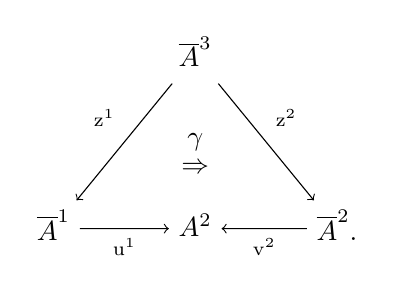
\begin{tikzpicture}[xscale=1.8,yscale=-1.1]
    \node (A0_1) at (0, 2) {$\overline{A}^1_{\CATA}$};
    \node (A1_0) at (1, 0) {$\overline{A}^3_{\CATA}$};
    \node (A1_1) at (1, 1) {$\gamma_{\CATA}$};
    \node (B1_1) at (1, 1.3) {$\Rightarrow$};
    \node (A1_2) at (1, 2) {$A^2_{\CATA}$};
    \node (A2_1) at (2, 2) {$\overline{A}^2_{\CATA}$.};
    
    \path (A1_0) edge [->]node [auto,swap] {$\scriptstyle{\operatorname{z}^1_{\CATA}}$} (A0_1);
    \path (A1_0) edge [->]node [auto] {$\scriptstyle{\operatorname{z}^2_{\CATA}}$} (A2_1);
    \path (A0_1) edge [->]node [auto,swap] {$\scriptstyle{\operatorname{u}^1_{\CATA}}$} (A1_2);
    \path (A2_1) edge [->]node [auto] {$\scriptstyle{\operatorname{v}^2_{\CATA}}$} (A1_2);
\end{tikzpicture}
\end{equation}

Then $\Gamma^2_{\CATA}\odot\Gamma^1_{\CATA}$ is represented by the data in the following diagram:

\[
\begin{tikzpicture}[xscale=2.8,yscale=-1.8]
    \node (A0_2) at (2, 0) {$A^1_{\CATA}$};
    \node (A2_2) at (2, 2) {$\overline{A}^3_{\CATA}$};
    \node (A1_2) at (2, 1) {$\overline{A}^1_{\CATA}$};
    \node (A3_2) at (2, 3) {$\overline{A}^2_{\CATA}$};
    \node (A2_1) at (1, 2) {$A^2_{\CATA}$};
    \node (A2_3) at (3, 2) {$A^2_{\CATA}$};
    \node (A2_0) at (0, 2) {$A_{\CATA}$};
    \node (A2_4) at (4, 2) {$B_{\CATA}$.};
    \node (A4_2) at (2, 4) {$A^3_{\CATA}$};
    
    \node (B1_1) at (0.9, 1.6) {$\Downarrow\,\alpha^1_{\CATA}$};
    \node (B2_2) at (0.9, 2.4) {$\Downarrow\,\alpha^2_{\CATA}$};
    \node (C1_1) at (3.1, 1.6) {$\Downarrow\,\beta^1_{\CATA}$};
    \node (C2_2) at (3.1, 2.4) {$\Downarrow\,\beta^2_{\CATA}$};
    \node (D1_1) at (1.6, 2) {$\Downarrow\,\gamma_{\CATA}$};
    \node (D2_2) at (2.4, 2) {$\Downarrow\,\gamma_{\CATA}$};
 
    \path (A4_2) edge [->]node [auto,swap] {$\scriptstyle{f^3_{\CATA}}$} (A2_4);
    \path (A0_2) edge [->]node [auto] {$\scriptstyle{f^1_{\CATA}}$} (A2_4);
    \path (A2_2) edge [->]node [auto] {$\scriptstyle{\operatorname{z}^1_{\CATA}}$} (A1_2);
    \path (A1_2) edge [->]node [auto,swap] {$\scriptstyle{\operatorname{v}^1_{\CATA}}$} (A0_2);
    \path (A2_2) edge [->]node [auto,swap] {$\scriptstyle{\operatorname{z}^2_{\CATA}}$} (A3_2);
    \path (A3_2) edge [->]node [auto] {$\scriptstyle{\operatorname{u}^2_{\CATA}}$} (A4_2);
    \path (A4_2) edge [->]node [auto] {$\scriptstyle{\operatorname{w}^3_{\CATA}}$} (A2_0);
    \path (A0_2) edge [->]node [auto,swap] {$\scriptstyle{\operatorname{w}^1_{\CATA}}$} (A2_0);
    \path (A1_2) edge [->]node [auto,swap] {$\scriptstyle{\operatorname{u}^1_{\CATA}}$} (A2_1);
    \path (A3_2) edge [->]node [auto] {$\scriptstyle{\operatorname{v}^2_{\CATA}}$} (A2_1);
    \path (A1_2) edge [->]node [auto] {$\scriptstyle{\operatorname{u}^1_{\CATA}}$} (A2_3);
    \path (A3_2) edge [->]node [auto,swap] {$\scriptstyle{\operatorname{v}^2_{\CATA}}$} (A2_3);
    \path (A2_1) edge [->]node [auto] {$\scriptstyle{\operatorname{w}^2_{\CATA}}$} (A2_0);
    \path (A2_3) edge [->]node [auto,swap] {$\scriptstyle{f^2_{\CATA}}$} (A2_4);
\end{tikzpicture}
\]

Since we are assuming that $\functor{F}$ is a strict pseudofunctor, then $\functor{N}_2
(\Gamma^2_{\CATA}\odot\Gamma^1_{\CATA})$ is represented by the following diagram:

\begin{equation}\label{eq-118}
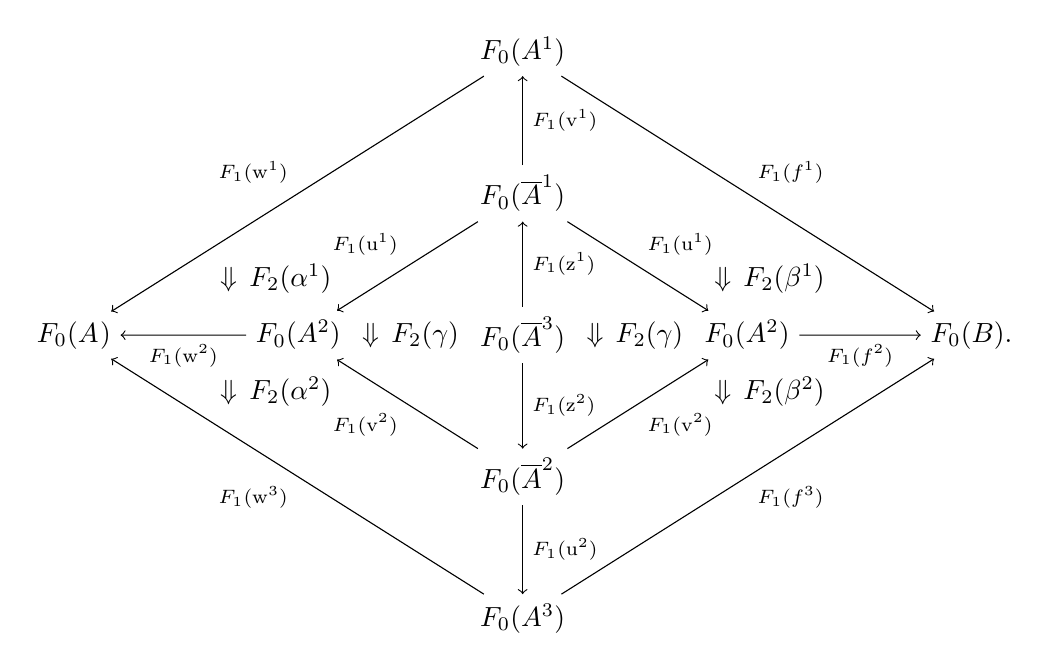
\begin{tikzpicture}[xscale=2.85,yscale=-1.8]
    \node (A0_2) at (2, 0) {$\functor{F}_0(A^1_{\CATA})$};
    \node (A2_2) at (2, 2) {$\functor{F}_0(\overline{A}^3_{\CATA})$};
    \node (A1_2) at (2, 1) {$\functor{F}_0(\overline{A}^1_{\CATA})$};
    \node (A3_2) at (2, 3) {$\functor{F}_0(\overline{A}^2_{\CATA})$};
    \node (A2_1) at (1, 2) {$\functor{F}_0(A^2_{\CATA})$};
    \node (A2_3) at (3, 2) {$\functor{F}_0(A^2_{\CATA})$};
    \node (A2_0) at (0, 2) {$\functor{F}_0(A_{\CATA})$};
    \node (A2_4) at (4, 2) {$\functor{F}_0(B_{\CATA})$.};
    \node (A4_2) at (2, 4) {$\functor{F}_0(A^3_{\CATA})$};

    \node (B1_1) at (0.9, 1.6) {$\Downarrow\,\functor{F}_2(\alpha^1_{\CATA})$};
    \node (B2_2) at (0.9, 2.4) {$\Downarrow\,\functor{F}_2(\alpha^2_{\CATA})$};
    \node (C1_1) at (3.1, 1.6) {$\Downarrow\,\functor{F}_2(\beta^1_{\CATA})$};
    \node (C2_2) at (3.1, 2.4) {$\Downarrow\,\functor{F}_2(\beta^2_{\CATA})$};
    \node (D1_1) at (1.5, 2) {$\Downarrow\,\functor{F}_2(\gamma_{\CATA})$};
    \node (D2_2) at (2.5, 2) {$\Downarrow\,\functor{F}_2(\gamma_{\CATA})$};
 
    \path (A4_2) edge [->]node [auto,swap] {$\scriptstyle{\functor{F}_1(f^3_{\CATA})}$} (A2_4);
    \path (A0_2) edge [->]node [auto] {$\scriptstyle{\functor{F}_1(f^1_{\CATA})}$} (A2_4);
    \path (A2_2) edge [->]node [auto,swap]
      {$\scriptstyle{\functor{F}_1(\operatorname{z}^1_{\CATA})}$} (A1_2);
    \path (A1_2) edge [->]node [auto,swap]
      {$\scriptstyle{\functor{F}_1(\operatorname{v}^1_{\CATA})}$} (A0_2);
    \path (A2_2) edge [->]node [auto]
      {$\scriptstyle{\functor{F}_1(\operatorname{z}^2_{\CATA})}$} (A3_2);
    \path (A3_2) edge [->]node [auto]
      {$\scriptstyle{\functor{F}_1(\operatorname{u}^2_{\CATA})}$} (A4_2);
    \path (A4_2) edge [->]node [auto]
      {$\scriptstyle{\functor{F}_1(\operatorname{w}^3_{\CATA})}$} (A2_0);
    \path (A0_2) edge [->]node [auto,swap]
      {$\scriptstyle{\functor{F}_1(\operatorname{w}^1_{\CATA})}$} (A2_0);
    \path (A1_2) edge [->]node [auto,swap]
      {$\scriptstyle{\functor{F}_1(\operatorname{u}^1_{\CATA})}$} (A2_1);
    \path (A3_2) edge [->]node [auto]
      {$\scriptstyle{\functor{F}_1(\operatorname{v}^2_{\CATA})}$} (A2_1);
    \path (A1_2) edge [->]node [auto]
      {$\scriptstyle{\functor{F}_1(\operatorname{u}^1_{\CATA})}$} (A2_3);
    \path (A3_2) edge [->]node [auto,swap]
      {$\scriptstyle{\functor{F}_1(\operatorname{v}^2_{\CATA})}$} (A2_3);
    \path (A2_1) edge [->]node [auto]
      {$\scriptstyle{\functor{F}_1(\operatorname{w}^2_{\CATA})}$} (A2_0);
    \path (A2_3) edge [->]node [auto,swap]
      {$\scriptstyle{\functor{F}_1(f^2_{\CATA})}$} (A2_4);
\end{tikzpicture}
\end{equation}

Now let us consider the following diagram:

\begin{equation}\label{eq-104}
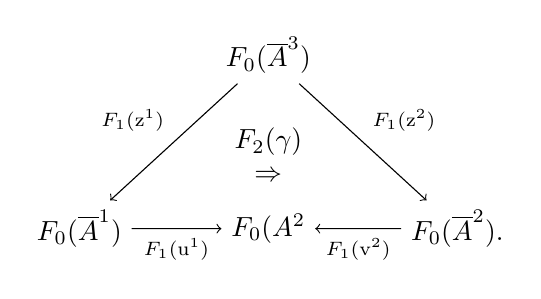
\begin{tikzpicture}[xscale=2.4,yscale=-1.1]
    \node (A0_1) at (0, 2) {$\functor{F}_0(\overline{A}^1_{\CATA})$};
    \node (A1_0) at (1, 0) {$\functor{F}_0(\overline{A}^3_{\CATA})$};
    \node (A1_2) at (1, 2) {$\functor{F}_0(A^2_{\CATA}$};
    \node (A2_1) at (2, 2) {$\functor{F}_0(\overline{A}^2_{\CATA})$.};
    
    \node (A1_1) at (1, 1) {$\functor{F}_2(\gamma_{\CATA})$};
    \node (B1_1) at (1, 1.4) {$\Rightarrow$};
    
    \path (A1_0) edge [->]node [auto,swap] {$\scriptstyle{\functor{F}_1(\operatorname{z}^1_{\CATA})}$} (A0_1);
    \path (A1_0) edge [->]node [auto] {$\scriptstyle{\functor{F}_1(\operatorname{z}^2_{\CATA})}$} (A2_1);
    \path (A0_1) edge [->]node [auto,swap] {$\scriptstyle{\functor{F}_1(\operatorname{u}^1_{\CATA})}$} (A1_2);
    \path (A2_1) edge [->]node [auto] {$\scriptstyle{\functor{F}_1(\operatorname{v}^2_{\CATA})}$} (A1_2);
\end{tikzpicture}
\end{equation}

By hypothesis, $\functor{F}_1(\operatorname{z}^1_{\CATA})$ belongs to $\SETWBsat$; moreover
$\functor{F}_2(\gamma_{\CATA})$ is invertible because $\gamma_{\CATA}$ is so. Therefore,
by~\cite[Proposition~0.2]{T3} for $(\CATC,\SETW):=(\CATB,\SETWBsat)$, using diagram \eqref{eq-104}
we conclude that diagram \eqref{eq-118} represents
$\functor{N}_2(\Gamma^2_{\CATA})\odot\functor{N}_2
(\Gamma^1_{\CATA})$, so we are done.
\end{proof}

\section{$\functor{N}$ is compatible with associators}
To say that $\functor{N}$ is compatible with associators is equivalent to proving the
following:

\begin{lem}
Given any triple of morphisms $\underline{f}_{\CATA},\underline{g}_{\CATA},\underline{h}_{\CATA}$ as in
\eqref{eq-114}, the composition of the following $2$-morphisms

\begin{equation}\label{eq-179}
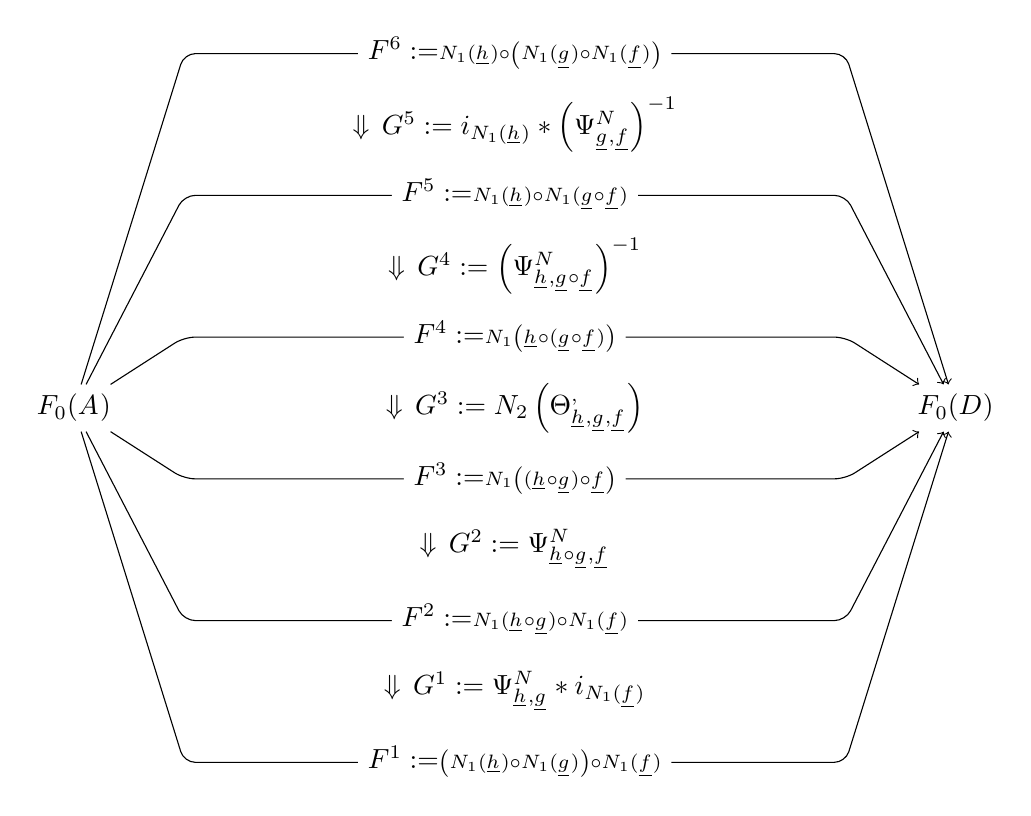
\begin{tikzpicture}[xscale=2.8,yscale=-1.8]
    \node (A2_0) at (0, 2.5) {$\functor{F}_0(A_{\CATA})$};
    \node (A2_3) at (4, 2.5) {$\functor{F}_0(D_{\CATA})$};

    \node (A1_1) at (2, 0.5) {$\Downarrow\,G^5_{\CATB}:=i_{\functor{N}_1
      (\underline{h}_{\CATA})}\ast\left(\Psi^{\functor{N}}_{\underline{g}_{\CATA},
      \underline{f}_{\CATA}}\right)^{-1}$};
    \node (A2_1) at (2, 1.5) {$\Downarrow\,G^4_{\CATB}:=
      \left(\Psi^{\functor{N}}_{\underline{h}_{\CATA},
      \underline{g}_{\CATA}\circ\underline{f}_{\CATA}}\right)^{-1}$};
    \node (A3_1) at (2, 2.5) {$\Downarrow\,G^3_{\CATB}:=\functor{N}_2
      \left(\Theta^{\CATA,\SETWA}_{\underline{h}_{\CATA},
      \underline{g}_{\CATA},\underline{f}_{\CATA}}\right)$};
    \node (A4_1) at (2, 3.5) {$\Downarrow\,G^2_{\CATB}:=
      \Psi^{\functor{N}}_{\underline{h}_{\CATA}
      \circ\underline{g}_{\CATA},\underline{f}_{\CATB}}$};
    \node (A5_1) at (2, 4.5) {$\Downarrow\,G^1_{\CATB}:=
      \Psi^{\functor{N}}_{\underline{h}_{\CATA},
      \underline{g}_{\CATA}}\ast i_{\functor{N}_1(\underline{f}_{\CATA})}$};

    \foreach \i in {0,...,5} {\draw[rounded corners,->] (A2_0) to (0.5,\i) to (3.5,\i) to (A2_3);}

    \node[color=black,draw=white,fill=white,shape=rectangle,rounded corners=0.5ex,text centered]
      at (2, 0) {$F^6_{\CATB}:=\scriptstyle{\functor{N}_1
      (\underline{h}_{\CATA})\circ\left(\functor{N}_1(\underline{g}_{\CATA})\circ
       \functor{N}_1(\underline{f}_{\CATA})\right)}$};
    \node[color=black,draw=white,fill=white,shape=rectangle,rounded corners=0.5ex,text centered]
      at (2, 1) {$F^5_{\CATB}:=\scriptstyle{\functor{N}_1
      (\underline{h}_{\CATA})\circ\functor{N}_1(\underline{g}_{\CATA}\circ
      \underline{f}_{\CATA})}$};
    \node[color=black,draw=white,fill=white,shape=rectangle,rounded corners=0.5ex,text centered]
      at (2, 2) {$F^4_{\CATB}:=\scriptstyle{\functor{N}_1
      \left(\underline{h}_{\CATA}\circ(\underline{g}_{\CATA}\circ\underline{f}_{\CATA})\right)}$};
    \node[color=black,draw=white,fill=white,shape=rectangle,rounded corners=0.5ex,text centered]
      at (2, 3) {$F^3_{\CATB}:=\scriptstyle{\functor{N}_1
      \left((\underline{h}_{\CATA}\circ\underline{g}_{\CATA})\circ\underline{f}_{\CATA}\right)}$};
    \node[color=black,draw=white,fill=white,shape=rectangle,rounded corners=0.5ex,text centered]
      at (2, 4) {$F^2_{\CATB}:=\scriptstyle{\functor{N}_1
      (\underline{h}_{\CATA}\circ\underline{g}_{\CATA})\circ\functor{N}_1
      (\underline{f}_{\CATA})}$};
    \node[color=black,draw=white,fill=white,shape=rectangle,rounded corners=0.5ex,text centered]
      at (2, 5) {$F^1_{\CATB}:=\scriptstyle{\left(\functor{N}_1
     (\underline{h}_{\CATA})\circ\functor{N}_1(\underline{g}_{\CATA})\right)\circ
     \functor{N}_1(\underline{f}_{\CATA})}$};
\end{tikzpicture}
\end{equation}
%
coincides with the associator $\Theta^{\CATB,\SETWBsat}_{\functor{N}_1
(\underline{h}_{\CATA}),\functor{N}_1(\underline{g}_{\CATA}),\functor{N}_1
(\underline{f}_{\CATA})}$.
\end{lem}

Here the $2$-morphisms $\Psi_{\bullet}^{\functor{N}}$ are defined as in \eqref{eq-190},
the associator $\Theta^{\CATA,\SETWA}_{\bullet}$ is computed as in Proposition~\ref{prop-01}
and the associator $\Theta^{\CATB,\SETWBsat}_{\bullet}$ can be obtained analogously.

\begin{proof}
We already assume all the notations of \eqref{eq-187} and \eqref{eq-188}, so that identities
\eqref{eq-182} and \eqref{eq-183} hold. First of all, we compute the morphisms $F^1_{\CATB},
\cdots,F^6_{\CATB}$ mentioned above.\\

Let us suppose that choices C$(\SETWBsat)$
give data as in the upper
parts of the following $2$ polygons (starting from the smaller one), with $\operatorname{u}^1_{\CATB}$
and $\operatorname{u}^2_{\CATB}$ in $\SETWBsat$ and $\delta_{\CATB}$ and $\sigma_{\CATB}$ invertible:

\begin{equation}\label{eq-192}
\begin{tikzpicture}[xscale=2.3,yscale=-0.8]

    \def\formaa#1#2#3
    {\begin{scope}[shift={#1}, scale=#2]
    \draw [fill=#3, draw=white, line width=0pt, rounded corners] (3.5, 1.5) -- (5, 6) -- (3, 6) -- (2, 3.5) -- cycle;
    \end{scope}}

    \formaa{(0,0)}{1}{mypaleblue}
    \formaa{(0.95, 1.2)}{0.7}{white}

    %%%
    
    \def\formab#1#2#3
    {\begin{scope}[shift={#1}, scale=#2]
    \draw [fill=#3, draw=white, line width=0pt, rounded corners] (1, 6) -- (2, 3.5) -- (3, 6) -- cycle;
    \end{scope}}

    \formab{(0,0)}{1}{mypalelime}
    \formab{(0.6, 1.5)}{0.7}{white}
    
    %%%

    \node (A0_4) at (3.5, 1.5) {$A^2_{\CATB}$};
    \node (A3_2) at (2, 3.5) {$A^1_{\CATB}$};
    \node (A6_1) at (1, 6) {$\functor{F}_0(A'_{\CATA})$};
    \node (A6_2) at (2, 6) {$\functor{F}_0(B_{\CATA})$};
    \node (A6_3) at (3, 6) {$\functor{F}_0(B'_{\CATA})$};
    \node (A6_4) at (4, 6) {$\functor{F}_0(C_{\CATA})$};
    \node (A6_5) at (5, 6) {$\functor{F}_0(C'_{\CATA})$.};
    
    \node (A3_4) at (3.4, 4.5) {$\Rightarrow$};
    \node (A5_2) at (2, 5.2) {$\Rightarrow$};
    \node (A4_2) at (2, 4.7) {$\delta_{\CATB}$};
    \node (A2_4) at (3.4, 4) {$\sigma_{\CATB}$};

    \path (A3_2) edge [->]node [auto] {$\scriptstyle{f^1_{\CATB}}$} (A6_3);
    \path (A6_5) edge [->]node [auto] {$\scriptstyle{\functor{F}_1
      (\operatorname{w}_{\CATA})}$} (A6_4);
    \path (A6_1) edge [->]node [auto,swap] {$\scriptstyle{\functor{F}_1(f_{\CATA})}$} (A6_2);
    \path (A0_4) edge [->]node [auto] {$\scriptstyle{l_{\CATB}}$} (A6_5);
    \path (A0_4) edge [->]node [auto,swap] {$\scriptstyle{\operatorname{u}^2_{\CATB}}$} (A3_2);
    \path (A3_2) edge [->]node [auto,swap] {$\scriptstyle{\operatorname{u}^1_{\CATB}}$} (A6_1);
    \path (A6_3) edge [->]node [auto,swap] {$\scriptstyle{\functor{F}_1(g_{\CATA})}$} (A6_4);
    \path (A6_3) edge [->]node [auto] {$\scriptstyle{\functor{F}_1
      (\operatorname{v}_{\CATA})}$} (A6_2);
\end{tikzpicture}
\end{equation}

Then we have

\[
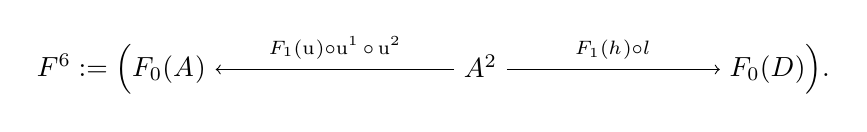
\begin{tikzpicture}[xscale=3.8,yscale=-1.2]
    \node (A0_0) at (-0.2, 0) {$F^6_{\CATB}:=\Big(\functor{F}_0(A_{\CATA})$};
    \node (A0_1) at (1, 0) {$A^2_{\CATB}$};
    \node (A0_2) at (2, 0) {$\functor{F}_0(D_{\CATA})\Big)$.};
    \path (A0_1) edge [->]node [auto,swap] {$\scriptstyle{\functor{F}_1(\operatorname{u}_{\CATA})
      \circ\operatorname{u}^1_{\CATB}\circ\operatorname{u}^2_{\CATB}}$} (A0_0);
    \path (A0_1) edge [->]node [auto] {$\scriptstyle{\functor{F}_1(h_{\CATA})
      \circ l_{\CATB}}$} (A0_2);
\end{tikzpicture}
\]

Moreover, let us suppose that choices C$(\SETWBsat)$
give data as in the upper part of the following diagram, with
$\widetilde{\operatorname{u}}^2_{\CATB}$ in $\SETWBsat$ and $\widetilde{\sigma}_{\CATB}$ invertible:

\[
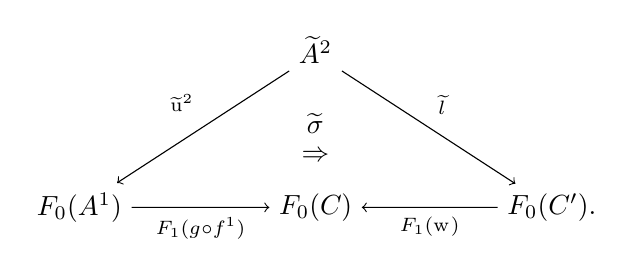
\begin{tikzpicture}[xscale=3.0,yscale=-1.3]
    \node (A0_1) at (1, 0.5) {$\widetilde{A}^2_{\CATB}$};
    \node (A1_0) at (0, 2) {$\functor{F}_0(A^1_{\CATA})$};
    \node (A1_1) at (1, 1.2) {$\widetilde{\sigma}_{\CATB}$};
    \node (B1_1) at (1, 1.5) {$\Rightarrow$};
    \node (A1_2) at (2, 2) {$\functor{F}_0(C'_{\CATA})$.};
    \node (A2_1) at (1, 2) {$\functor{F}_0(C_{\CATA})$};
    \path (A1_2) edge [->]node [auto]
      {$\scriptstyle{\functor{F}_1(\operatorname{w}_{\CATA})}$} (A2_1);
    \path (A0_1) edge [->]node [auto] {$\scriptstyle{\widetilde{l}_{\CATB}}$} (A1_2);
    \path (A1_0) edge [->]node [auto,swap]
      {$\scriptstyle{\functor{F}_1(g_{\CATA}\circ f^1_{\CATA})}$} (A2_1);
    \path (A0_1) edge [->]node [auto,swap]
      {$\scriptstyle{\widetilde{\operatorname{u}}^2_{\CATB}}$} (A1_0);
\end{tikzpicture}
\]

Then we have

\[
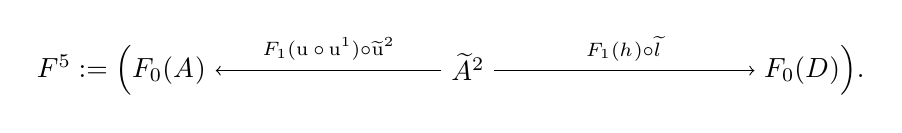
\begin{tikzpicture}[xscale=4.4,yscale=-1.2]
    \node (A0_0) at (0, 0) {$F^5_{\CATB}:=\Big(\functor{F}_0(A_{\CATA})$};
    \node (A0_1) at (1, 0) {$\widetilde{A}^2_{\CATB}$};
    \node (A0_2) at (2, 0) {$\functor{F}_0(D_{\CATA})\Big)$.};
    \path (A0_1) edge [->]node [auto,swap] {$\scriptstyle{\functor{F}_1(\operatorname{u}_{\CATA}
      \circ\operatorname{u}^1_{\CATA})\circ\widetilde{\operatorname{u}}^2_{\CATB}}$} (A0_0);
    \path (A0_1) edge [->]node [auto] {$\scriptstyle{\functor{F}_1(h_{\CATA})\circ
      \widetilde{l}_{\CATB}}$} (A0_2);
\end{tikzpicture}
\]

Using \eqref{eq-182} and \eqref{eq-183}, we have

\[
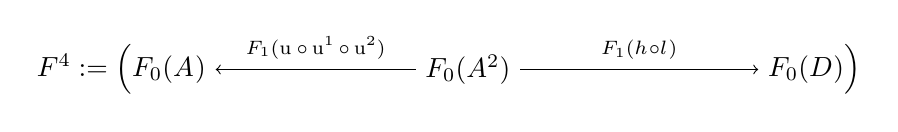
\begin{tikzpicture}[xscale=4.4,yscale=-1.2]
    \node (A0_0) at (0, 0) {$F^4_{\CATB}:=\Big(\functor{F}_0(A_{\CATA})$};
    \node (A0_1) at (1, 0) {$\functor{F}_0(A^2_{\CATA})$};
    \node (A0_2) at (2, 0) {$\functor{F}_0(D_{\CATA})\Big)$};
    \path (A0_1) edge [->]node [auto,swap] {$\scriptstyle{\functor{F}_1(\operatorname{u}_{\CATA}
      \circ\operatorname{u}^1_{\CATA}\circ\operatorname{u}^2_{\CATA})}$} (A0_0);
    \path (A0_1) edge [->]node [auto]
      {$\scriptstyle{\functor{F}_1(h_{\CATA}\circ l_{\CATA})}$} (A0_2);
\end{tikzpicture}
\]
%
and

\[
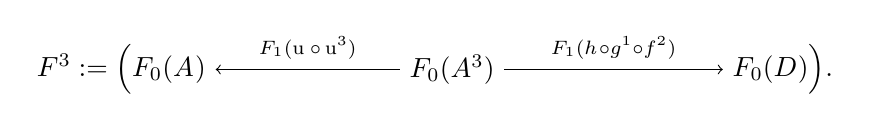
\begin{tikzpicture}[xscale=4.2,yscale=-1.2]
    \node (A0_0) at (0, 0) {$F^3_{\CATB}:=\Big(\functor{F}_0(A_{\CATA})$};
    \node (A0_1) at (1, 0) {$\functor{F}_0(A^3_{\CATA})$};
    \node (A0_2) at (2, 0) {$\functor{F}_0(D_{\CATA})\Big)$.};
    \path (A0_1) edge [->]node [auto,swap] {$\scriptstyle{\functor{F}_1(\operatorname{u}_{\CATA}
      \circ\operatorname{u}^3_{\CATA})}$} (A0_0);
    \path (A0_1) edge [->]node [auto]
      {$\scriptstyle{\functor{F}_1(h_{\CATA}\circ g^1_{\CATA}\circ f^2_{\CATA})}$} (A0_2);
\end{tikzpicture}
\]

Let us suppose that choices C$(\SETWBsat)$ give data as in the upper part of the following
diagram, with $\widetilde{\operatorname{u}}^3_{\CATB}$ in $\SETWBsat$ and $\widetilde{\eta}_{\CATB}$
invertible:

\[
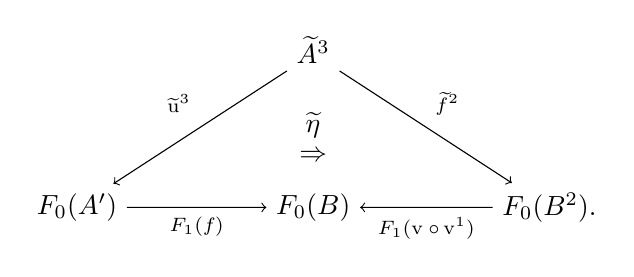
\begin{tikzpicture}[xscale=3.0,yscale=-1.3]
    \twocolorsdiagonal{mypaleorange}{mypaleyellow}{(1, 0.5) -- (2, 2) -- (0, 2) -- cycle}

    \node (A0_1) at (1, 0.5) {$\widetilde{A}^3_{\CATB}$};
    \node (A1_0) at (0, 2) {$\functor{F}_0(A'_{\CATA})$};
    \node (A1_2) at (2, 2) {$\functor{F}_0(B^2_{\CATA})$.};
    \node (A2_1) at (1, 2) {$\functor{F}_0(B_{\CATA})$};
    
    \node (A1_1) at (1, 1.2) {$\widetilde{\eta}_{\CATB}$};
    \node (B1_1) at (1, 1.5) {$\Rightarrow$};
    
    \path (A1_2) edge [->]node [auto] {$\scriptstyle{\functor{F}_1(\operatorname{v}_{\CATA}
      \circ\operatorname{v}^1_{\CATA})}$} (A2_1);
    \path (A0_1) edge [->]node [auto] {$\scriptstyle{\widetilde{f}^2_{\CATB}}$} (A1_2);
    \path (A1_0) edge [->]node [auto,swap] {$\scriptstyle{\functor{F}_1(f_{\CATA})}$} (A2_1);
    \path (A0_1) edge [->]node [auto,swap]
      {$\scriptstyle{\widetilde{\operatorname{u}}^3_{\CATB}}$} (A1_0);
\end{tikzpicture}
\]

Then we have

\[
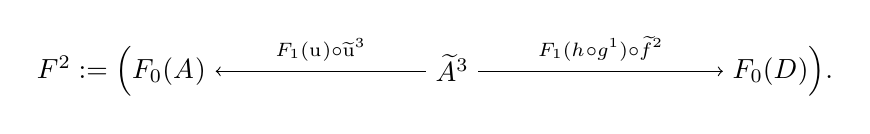
\begin{tikzpicture}[xscale=4.2,yscale=-1.2]
    \node (A0_0) at (0, 0) {$F^2_{\CATB}:=\Big(\functor{F}_0(A_{\CATA})$};
    \node (A0_1) at (1, 0) {$\widetilde{A}^3_{\CATB}$};
    \node (A0_2) at (2, 0) {$\functor{F}_0(D_{\CATA})\Big)$.};
    \path (A0_1) edge [->]node [auto,swap] {$\scriptstyle{\functor{F}_1(\operatorname{u}_{\CATA})
      \circ\widetilde{\operatorname{u}}^3_{\CATB}}$} (A0_0);
    \path (A0_1) edge [->]node [auto] {$\scriptstyle{\functor{F}_1(h_{\CATA}
      \circ g^1_{\CATA})\circ\widetilde{f}^2_{\CATB}}$} (A0_2);
\end{tikzpicture}
\]

Lastly, let us suppose that choices C$(\SETWBsat)$ give data as in the upper parts of the
following $2$ polygons (starting from the smaller one), with $\operatorname{v}^1_{\CATB}$ and
$\operatorname{u}^3_{\CATB}$ in $\SETWBsat$ and $\xi_{\CATB}$ and $\eta_{\CATB}$ invertible:

\begin{equation}\label{eq-193}
\begin{tikzpicture}[xscale=-2.3,yscale=-0.8]

    \def\formaa#1#2#3
    {\begin{scope}[shift={#1}, scale=#2]
    \draw [fill=#3, draw=white, line width=0pt, rounded corners] (3.5, 1.5) -- (5, 6) -- (3, 6) -- (2, 3.5) -- cycle;
    \end{scope}}

    \formaa{(0,0)}{1}{mypalered}
    \formaa{(0.95, 1.2)}{0.7}{white}

    %%%
    
    \def\formab#1#2#3
    {\begin{scope}[shift={#1}, scale=#2]
    \draw [fill=#3, draw=white, line width=0pt, rounded corners] (1, 6) -- (2, 3.5) -- (3, 6) -- cycle;
    \end{scope}}

    \formab{(0,0)}{1}{mypaleyellow}
    \formab{(0.6, 1.5)}{0.7}{white}
    
    %%%

    \node (A0_4) at (3.5, 1.5) {$A^3_{\CATB}$};
    \node (A3_2) at (2, 3.5) {$B^2_{\CATB}$};
    \node (A6_1) at (1, 6) {$\functor{F}_0(C'_{\CATA})$.};
    \node (A6_2) at (2, 6) {$\functor{F}_0(C_{\CATA})$};
    \node (A6_3) at (3, 6) {$\functor{F}_0(B'_{\CATA})$};
    \node (A6_4) at (4, 6) {$\functor{F}_0(B_{\CATA})$};
    \node (A6_5) at (5, 6) {$\functor{F}_0(A'_{\CATA})$};
    
    \node (A3_4) at (3.5, 4.5) {$\Rightarrow$};
    \node (A5_2) at (2, 5.2) {$\Rightarrow$};

    \node (A4_2) at (2, 4.7) {$\xi_{\CATB}$};
    \node (A2_4) at (3.5, 4) {$\eta_{\CATB}$};
    
    \path (A3_2) edge [->]node [auto,swap] {$\scriptstyle{\operatorname{v}^1_{\CATB}}$} (A6_3);
    \path (A6_5) edge [->]node [auto,swap] {$\scriptstyle{\functor{F}_1(f_{\CATA})}$} (A6_4);
    \path (A6_1) edge [->]node [auto] {$\scriptstyle{\functor{F}_1
      (\operatorname{w}_{\CATA})}$} (A6_2);
    \path (A0_4) edge [->]node [auto,swap] {$\scriptstyle{\operatorname{u}^3_{\CATB}}$} (A6_5);
    \path (A0_4) edge [->]node [auto] {$\scriptstyle{f^2_{\CATB}}$} (A3_2);
    \path (A3_2) edge [->]node [auto] {$\scriptstyle{g^1_{\CATB}}$} (A6_1);
    \path (A6_3) edge [->]node [auto] {$\scriptstyle{\functor{F}_1(\operatorname{v}_{\CATA})}$} (A6_4);
    \path (A6_3) edge [->]node [auto,swap] {$\scriptstyle{\functor{F}_1(g_{\CATA})}$} (A6_2);
\end{tikzpicture}
\end{equation}

Then

\[
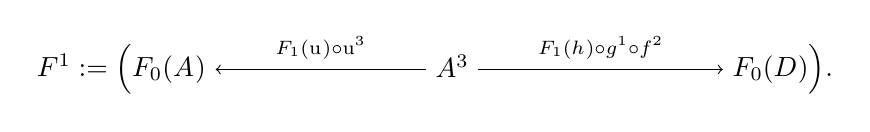
\begin{tikzpicture}[xscale=4.2,yscale=-1.2]
    \node (A0_0) at (0, 0) {$F^1_{\CATB}:=\Big(\functor{F}_0(A_{\CATA})$};
    \node (A0_1) at (1, 0) {$A^3_{\CATB}$};
    \node (A0_2) at (2, 0) {$\functor{F}_0(D_{\CATA})\Big)$.};
    \path (A0_1) edge [->]node [auto,swap] {$\scriptstyle{\functor{F}_1(\operatorname{u}_{\CATA})
      \circ\operatorname{u}^3_{\CATB}}$} (A0_0);
    \path (A0_1) edge [->]node [auto] {$\scriptstyle{\functor{F}_1(h_{\CATA})
      \circ g^1_{\CATB}\circ f^2_{\CATB}}$} (A0_2);
\end{tikzpicture}
\]

Now we compute the $2$-morphism $G^1_{\CATB}$ appearing in \eqref{eq-179}. We use (BF3)
for $(\CATB,\SETWBsat)$
in order to get data as in the upper part of the following diagram, with $\nu^1_{\CATB}$ invertible
and $\operatorname{z}^2_{\CATB}$ in $\SETWBsat$:

\[
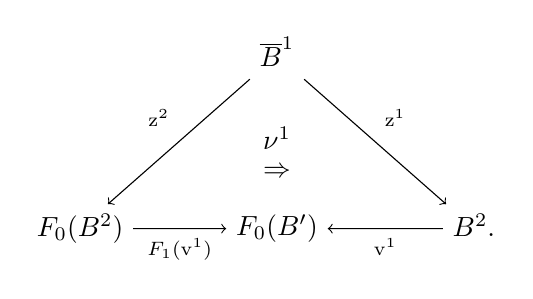
\begin{tikzpicture}[xscale=-2.5,yscale=-1.1]
    \twocolorsdiagonal{mypaleyellow}{mypaleolive}{(1, 0) -- (2, 2) -- (0, 2) -- cycle}
    
    \node (A0_1) at (0, 2) {$B^2_{\CATB}$.};
    \node (A1_0) at (1, 0) {$\overline{B}^1_{\CATB}$};
    \node (A1_2) at (1, 2) {$\functor{F}_0(B'_{\CATA})$};
    \node (A2_1) at (2, 2) {$\functor{F}_0(B^2_{\CATA})$};
    
    \node (A1_1) at (1, 1) {$\nu^1_{\CATB}$};
    \node (B1_1) at (1, 1.35) {$\Rightarrow$};
    
    \path (A1_0) edge [->]node [auto] {$\scriptstyle{\operatorname{z}^1_{\CATB}}$} (A0_1);
    \path (A1_0) edge [->]node [auto,swap] {$\scriptstyle{\operatorname{z}^2_{\CATB}}$} (A2_1);
    \path (A0_1) edge [->]node [auto] {$\scriptstyle{\operatorname{v}^1_{\CATB}}$} (A1_2);
    \path (A2_1) edge [->]node [auto,swap]
      {$\scriptstyle{\functor{F}_1(\operatorname{v}^1_{\CATA})}$} (A1_2);
\end{tikzpicture}
\]

We use axiom (BF4a) and (BF4b) for $(\CATB,\SETWBsat)$
in order to get an object $\overline{B}^2_{\CATB}$, a morphism
$\operatorname{z}^3_{\CATB}:\overline{B}^2_{\CATB}\rightarrow\overline{B}^1_{\CATB}$ in $\SETWBsat$
and an invertible $2$-morphism

\[
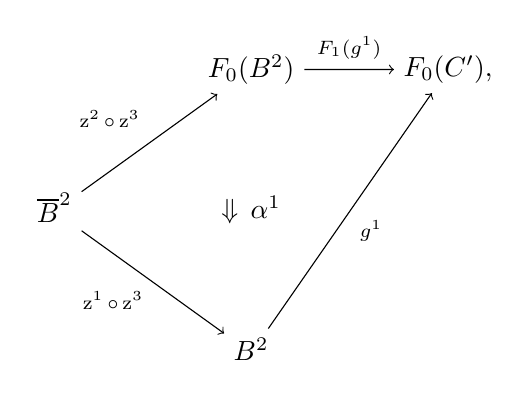
\begin{tikzpicture}[xscale=2.5,yscale=-1.8]
    \fillonecolor{mypaleolive}{(3, 3) -- (4, 2) -- (5, 2) -- (4, 4) -- cycle}

    \node (A3_3) at (3, 3) {$\overline{B}^2_{\CATB}$};
    \node (A2_4) at (4, 2) {$\functor{F}_0(B^2_{\CATA})$};
    \node (A2_5) at (5, 2) {$\functor{F}_0(C'_{\CATA})$,};
    \node (A4_4) at (4, 4) {$B^2_{\CATB}$};

    \node (A3_4) at (4, 3) {$\Downarrow\,\alpha^1_{\CATB}$};

    \path (A4_4) edge [->]node [auto,swap] {$\scriptstyle{g^1_{\CATB}}$} (A2_5);
    \path (A2_4) edge [->]node [auto] {$\scriptstyle{\functor{F}_1(g^1_{\CATA})}$} (A2_5);
    \path (A3_3) edge [->]node [auto,swap] {$\scriptstyle{\operatorname{z}^1_{\CATB}
      \circ\operatorname{z}^3_{\CATB}}$} (A4_4);        
    \path (A3_3) edge [->]node [auto] {$\scriptstyle{\operatorname{z}^2_{\CATB}
      \circ\operatorname{z}^3_{\CATB}}$} (A2_4);
\end{tikzpicture}
\]
%
such that $i_{\functor{F}_1(\operatorname{w}_{\CATA})}\ast\alpha^1_{\CATB}$ coincides with the
following composition

\begin{equation}\label{eq-125}
\begin{tikzpicture}[xscale=1.8, yscale=1.2]

    \def\formaa#1#2#3
    {\begin{scope}[shift={#1}, scale=#2]
    \draw [fill=#3, draw=white, line width=0pt, rounded corners] (3, 1) -- (5, 1)  -- (6, 3) -- (4, 3) -- cycle;
    \end{scope}}

    \formaa{(0,0)}{1}{mypalered}
    \formaa{(0.65, 0.3)}{0.85}{white}
    
    %%%

    \twocolorsdiagonal{mypalemagenta}{mypaleolive}{(3, 5) -- (5, 5)  -- (6, 3) -- (4, 3) -- cycle}
    \twocolorsdiagonal{mypaleyellow}{mypaleolive}{(2, 3) -- (3, 5)  -- (4, 3) -- (3, 1) -- cycle}
     
    %%%
    
    \node (A1_2) at (3, 1) {$B^2_{\CATB}$};
    \node (A1_5) at (5, 1) {$\functor{F}_0(C'_{\CATA})$};
    \node (A3_0) at (1, 3) {$\overline{B}^2_{\CATB}$};
    \node (A3_1) at (2, 3) {$\overline{B}^1_{\CATB}$};
    \node (A3_4) at (4, 3) {$\functor{F}_0(B'_{\CATA})$};
    \node (A3_6) at (6, 3) {$\functor{F}_0(C_{\CATA})$.};
    \node (A5_2) at (3, 5) {$\functor{F}_0(B^2_{\CATA})$};
    \node (A5_5) at (5, 5) {$\functor{F}_0(C'_{\CATA})$};

    \node (A3_2) at (2.8, 3) {$\Downarrow\,\nu^1_{\CATB}$};
    \node (A4_5) at (4.5, 4) {$\Downarrow\,\functor{F}_2(\xi_{\CATA})^{-1}$};
    \node (A2_5) at (4.5, 2) {$\Downarrow\,\xi_{\CATB}$};

    \path (A5_2) edge [->]node [auto,swap]
      {$\scriptstyle{\functor{F}_1(\operatorname{v}^1_{\CATA})}$} (A3_4);
    \path (A3_0) edge [->]node [auto] {$\scriptstyle{\operatorname{z}^3_{\CATB}}$} (A3_1);
    \path (A5_2) edge [->]node [auto] {$\scriptstyle{\functor{F}_1(g^1_{\CATA})}$} (A5_5);
    \path (A3_1) edge [->]node [auto] {$\scriptstyle{\operatorname{z}^2_{\CATB}}$} (A5_2);
    \path (A3_4) edge [->]node [auto] {$\scriptstyle{\functor{F}_1(g_{\CATA})}$} (A3_6);
    \path (A3_1) edge [->]node [auto,swap] {$\scriptstyle{\operatorname{z}^1_{\CATB}}$} (A1_2);
    \path (A1_2) edge [->]node [auto] {$\scriptstyle{\operatorname{v}^1_{\CATB}}$} (A3_4);
    \path (A5_5) edge [->]node [auto]
      {$\scriptstyle{\functor{F}_1(\operatorname{w}_{\CATA})}$} (A3_6);
    \path (A1_5) edge [->]node [auto,swap]
      {$\scriptstyle{\functor{F}_1(\operatorname{w}_{\CATA})}$} (A3_6);
    \path (A1_2) edge [->]node [auto,swap] {$\scriptstyle{g^1_{\CATB}}$} (A1_5);
\end{tikzpicture}
\end{equation}

Then by Lemma~\ref{lem-01} (and using the fact that we are assuming
that $\functor{F}$ is strict), $\Psi^{\functor{N}}_{\underline{h}_{\CATA},
\underline{g}_{\CATA}}$ is represented by the following diagram:

\begin{equation}\label{eq-178}
\begin{tikzpicture}[xscale=2.8,yscale=1.5]
    \node (A0_2) at (2, 0) {$B^2_
    {\CATB}$};
    \node (A2_2) at (2, 2) {$\overline{B}^2_{\CATB}$};
    \node (A2_4) at (4, 2) {$\functor{F}_0(D_{\CATA})$.};
    \node (A2_0) at (0, 2) {$\functor{F}_0(B_{\CATA})$};
    \node (A4_2) at (2, 4) {$\functor{F}_0(B^2_{\CATA})$};

    \node (A2_3) at (2.8, 2) {$\Downarrow\,i_{\functor{F}_1(h_{\CATA})}\ast\alpha^1_{\CATB}$};
    \node (A2_1) at (1.1, 2) {$\Downarrow\,i_{\functor{F}_1(\operatorname{v}_{\CATA})}\ast
      \nu^1_{\CATB}\ast i_{\operatorname{z}^3_{\CATB}}$};

    \path (A4_2) edge [->]node [auto]
       {$\scriptstyle{\functor{F}_1(h_{\CATA}\circ g^1_{\CATA})}$} (A2_4);
    \path (A0_2) edge [->]node [auto,swap]
      {$\scriptstyle{\functor{F}_1(h_{\CATA})\circ g^1_{\CATB}}$} (A2_4);
    \path (A4_2) edge [->]node [auto,swap] {$\scriptstyle{\functor{F}_1(\operatorname{v}_{\CATA}
      \circ\operatorname{v}^1_{\CATA})}$} (A2_0);
    \path (A0_2) edge [->]node [auto] {$\scriptstyle{\functor{F}_1(\operatorname{v}_{\CATA})
      \circ\operatorname{v}^1_{\CATB}}$} (A2_0);
    \path (A2_2) edge [->]node [auto] {$\scriptstyle{\operatorname{z}^1_{\CATB}
      \circ\operatorname{z}^3_{\CATB}}$} (A0_2);
    \path (A2_2) edge [->]node [auto,swap] {$\scriptstyle{\operatorname{z}^2_{\CATB}\circ
      \operatorname{z}^3_{\CATB}}$} (A4_2);
\end{tikzpicture}
\end{equation}

Now we use (BF3) for $(\CATB,\SETWBsat)$
in order to get data as in upper parts of
the following $2$ diagrams, with $\operatorname{z}^4_{\CATB}$ and $\operatorname{z}^5_{\CATB}$ in
$\SETWBsat$ and $\nu^2_{\CATB}$ and $\nu^3_{\CATB}$ invertible:

\[
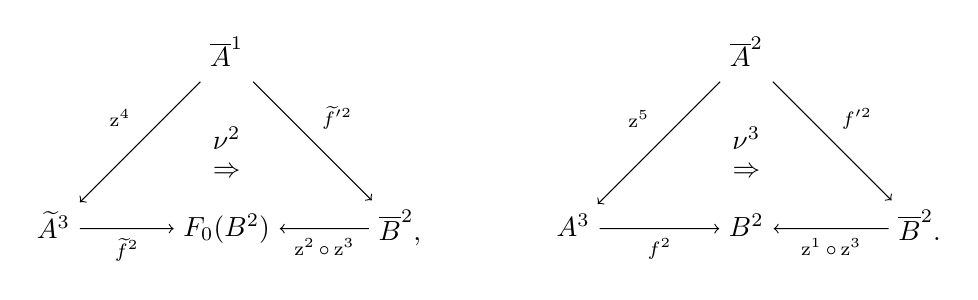
\begin{tikzpicture}[xscale=2.2,yscale=-1.1]
    \twocolorsdiagonal{mypalelime}{mypaleyellow}{(0, 2) -- (1, 0) -- (2, 2) -- cycle}
    \twocolorsdiagonal{mypalelime}{mypaleyellow}{(3, 2) -- (4, 0) -- (5, 2) -- cycle}

    \node (A0_1) at (0, 2) {$\widetilde{A}^3_{\CATB}$};
    \node (A1_0) at (1, 0) {$\overline{A}^1_{\CATB}$};
    \node (A1_2) at (1, 2) {$\functor{F}_0(B^2_{\CATA})$};
    \node (A2_1) at (2, 2) {$\overline{B}^2_{\CATB}$,};
    
    \node (A1_1) at (1, 1) {$\nu^2_{\CATB}$};
    \node (C1_1) at (1, 1.35) {$\Rightarrow$};
    
    \node (B0_1) at (3, 2) {$A^3_{\CATB}$};
    \node (B1_0) at (4, 0) {$\overline{A}^2_{\CATB}$};
    \node (B1_2) at (4, 2) {$B^2_{\CATB}$};
    \node (B2_1) at (5, 2) {$\overline{B}^2_{\CATB}$.};

    \node (B1_1) at (4, 1) {$\nu^3_{\CATB}$};
    \node (D1_1) at (4, 1.35) {$\Rightarrow$};
    
    \path (A1_0) edge [->]node [auto,swap] {$\scriptstyle{\operatorname{z}^4_{\CATB}}$} (A0_1);
    \path (A1_0) edge [->]node [auto] {$\scriptstyle{\widetilde{f}^{\prime 2}_{\CATB}}$} (A2_1);
    \path (A0_1) edge [->]node [auto,swap] {$\scriptstyle{\widetilde{f}^2_{\CATB}}$} (A1_2);
    \path (A2_1) edge [->]node [auto]
      {$\scriptstyle{\operatorname{z}^2_{\CATB}\circ\operatorname{z}^3_{\CATB}}$} (A1_2);
    
    \path (B1_0) edge [->]node [auto,swap] {$\scriptstyle{\operatorname{z}^5_{\CATB}}$} (B0_1);
    \path (B1_0) edge [->]node [auto] {$\scriptstyle{f^{\prime 2}_{\CATB}}$} (B2_1);
    \path (B0_1) edge [->]node [auto,swap] {$\scriptstyle{f^2_{\CATB}}$} (B1_2);
    \path (B2_1) edge [->]node [auto]
      {$\scriptstyle{\operatorname{z}^1_{\CATB}\circ\operatorname{z}^3_{\CATB}}$} (B1_2);
\end{tikzpicture}
\]

Then we use again (BF3) for $(\CATB,\SETWBsat)$
in order to get data as in the upper part of the following
diagram, with $\operatorname{z}^6_{\CATB}$ in $\SETWBsat$ and $\nu^4_{\CATB}$ invertible:

\[
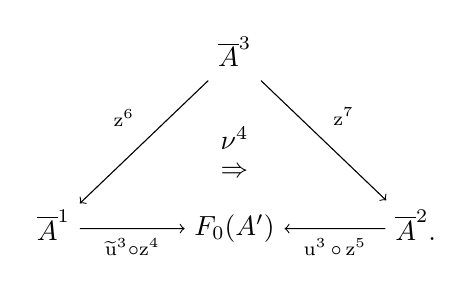
\begin{tikzpicture}[xscale=2.3,yscale=-1.1]
    \twocolorsdiagonal{mypaleyellow}{white}{(0, 2) -- (1, 0) -- (2, 2) -- cycle}

    \node (A0_1) at (0, 2) {$\overline{A}^1_{\CATB}$};
    \node (A1_0) at (1, 0) {$\overline{A}^3_{\CATB}$};
    \node (A1_2) at (1, 2) {$\functor{F}_0(A'_{\CATA})$};
    \node (A2_1) at (2, 2) {$\overline{A}^2_{\CATB}$.};
    
    \node (A1_1) at (1, 1) {$\nu^4_{\CATB}$};
    \node (B1_1) at (1, 1.35) {$\Rightarrow$};
    
    \path (A1_0) edge [->]node [auto,swap] {$\scriptstyle{\operatorname{z}^6_{\CATB}}$} (A0_1);
    \path (A1_0) edge [->]node [auto] {$\scriptstyle{\operatorname{z}^7_{\CATB}}$} (A2_1);
    \path (A0_1) edge [->]node [auto,swap] {$\scriptstyle{\widetilde{\operatorname{u}}^3_{\CATB}
      \circ\operatorname{z}^4_{\CATB}}$} (A1_2);
    \path (A2_1) edge [->]node [auto]
      {$\scriptstyle{\operatorname{u}^3_{\CATB}\circ\operatorname{z}^5_{\CATB}}$} (A1_2);
\end{tikzpicture}
\]

Now we use axioms (BF4a) and (BF4b) for $(\CATB,\SETWBsat)$
in order to get an object $\overline{A}^4_{\CATB}$, a morphism
$\operatorname{z}^8_{\CATB}:\overline{A}^4_{\CATB}\rightarrow\overline{A}^3_{\CATB}$ in $\SETWBsat$
and an invertible $2$-morphism

\[
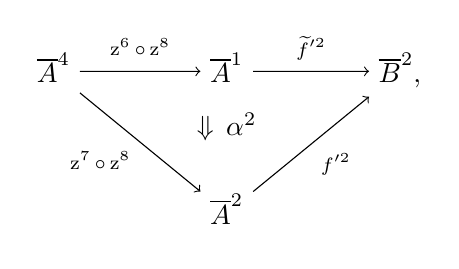
\begin{tikzpicture}[xscale=2.2, yscale=-1.8]
    \fillonecolor{mypaleyellow}{(4, 8)  --  (3, 7) -- (5, 7) -- cycle}
       
    \node (A8_5) at (4, 8) {$\overline{A}^2_{\CATB}$};
    \node (A7_5) at (5, 7) {$\overline{B}^2_{\CATB}$,};
    \node (A5_4) at (4, 7) {$\overline{A}^1_{\CATB}$};
    \node (A5_3) at (3, 7) {$\overline{A}^4_{\CATB}$};
 
    \node (C8_8) at (4, 7.4) {$\Downarrow\,\alpha^2_{\CATB}$};
 
    \path (A5_3) edge [->]node [auto] {$\scriptstyle{\operatorname{z}^6_{\CATB}
      \circ\operatorname{z}^8_{\CATB}}$} (A5_4);
    \path (A5_3) edge [->]node [auto,swap] {$\scriptstyle{\operatorname{z}^7_{\CATB}
      \circ\operatorname{z}^8_{\CATB}}$} (A8_5);
    \path (A5_4) edge [->]node [auto] {$\scriptstyle{\widetilde{f}^{\prime 2}_{\CATB}}$} (A7_5);
    \path (A8_5) edge [->]node [auto,swap] {$\scriptstyle{f^{\prime 2}_{\CATB}}$} (A7_5);
\end{tikzpicture}
\]
%
such that $i_{\functor{F}_1(\operatorname{v}_{\CATA}\circ\operatorname{v}^1_{\CATA})\circ
\operatorname{z}^2_{\CATB}\circ\operatorname{z}^3_{\CATB}}\ast\alpha^2_{\CATB}$ coincides with the
following composition

\begin{equation}\label{eq-136}
\begin{tikzpicture}[xscale=2.5, yscale=-1.2]
  
    \def\formaa#1#2#3
    {\begin{scope}[shift={#1}, scale=#2]
    \draw [fill=#3, draw=white, line width=0pt, rounded corners] (3, 4) -- (4, 3) -- (5, 3) -- (5, 5) -- (4, 5) -- cycle;
    \end{scope}}

    \formaa{(0,0)}{1}{mypaleyellow}
    \formaa{(1.3, 1.2)}{0.7}{white}
  
    %%%
    
    \twocolorsdiagonal{white}{mypaleyellow}{(1, 3) -- (2, 1)  -- (4, 3) -- (2, 5) -- cycle}

    \twocolorsdiagonal{mypalelime}{mypaleyellow}{(2, 1)  -- (3, 0) -- (4, 1) -- (3, 2) -- cycle}
    
    \twocolorsdiagonal{mypalelime}{mypaleyellow}{(2, 5)  -- (3, 4) -- (4, 5) -- (4, 6) -- (3,6) -- cycle}
    
    \twocolorsdiagonal{mypaleorange}{mypaleyellow}{(3, 2)  -- (4, 1) -- (5, 3) -- (4, 3) -- cycle}
    
    \twocolorsdiagonal{mypaleolive}{mypaleyellow}{(4, 6)  -- (4, 5) -- (5, 5) -- (5, 6) -- cycle}
     
    \node (A5_4) at (4, 5) {$B^2_{\CATB}$};
    \node (A6_3) at (3, 6) {$\overline{B}^2_{\CATB}$};
    \node (A6_4) at (5, 6) {$\functor{F}_0(B^2_{\CATA})$};
    \node (A3_5) at (5, 3) {$\functor{F}_0(B_{\CATA})$.};
    \node (B2_2) at (4, 6) {$\overline{B}^1_{\CATB}$};
    \node (B3_3) at (5, 5) {$\functor{F}_0(B'_{\CATA})$};
    \node (A1_4) at (4, 1) {$\functor{F}_0(B^2_{\CATA})$};   
    \node (A0_3) at (3, 0) {$\overline{B}^2_{\CATB}$};
    \node (A1_2) at (2, 1) {$\overline{A}^1_{\CATB}$};
    \node (A2_3) at (3, 2) {$\widetilde{A}^3_{\CATB}$};
    \node (A3_0) at (0.4, 3) {$\overline{A}^4_{\CATB}$};
    \node (A3_1) at (1, 3) {$\overline{A}^3_{\CATB}$};
    \node (A3_4) at (4, 3) {$\functor{F}_0(A'_{\CATA})$};
    \node (A4_3) at (3, 4) {$A^3_{\CATB}$};
    \node (A5_2) at (2, 5) {$\overline{A}^2_{\CATB}$};

    \node (A2_4) at (4, 2) {$\Downarrow\,\widetilde{\eta}_{\CATB}^{-1}$};
    \node (A5_3) at (3, 5) {$\Downarrow\,\nu^3_{\CATB}$};
    \node (A4_4) at (4.3, 4) {$\Downarrow\,\eta_{\CATB}$};
    \node (A5_5) at (4.4, 5.5) {$\Downarrow\,(\nu^1_{\CATB})^{-1}$};
    \node (A1_3) at (3, 1) {$\Downarrow\,(\nu^2_{\CATB})^{-1}$};
    \node (A3_2) at (2, 3) {$\Downarrow\,\nu^4_{\CATB}$};

    \path (A5_4) edge [->]node [auto] {$\scriptstyle{\operatorname{v}^1_{\CATB}}$} (B3_3);
    \path (B3_3) edge [->]node [auto,swap]
      {$\scriptstyle{\functor{F}_1(\operatorname{v}_{\CATA})}$} (A3_5);
    \path (A6_4) edge [->]node [auto,swap]
      {$\scriptstyle{\functor{F}_1(\operatorname{v}^1_{\CATA})}$} (B3_3);
    \path (A6_3) edge [->]node [auto,swap] {$\scriptstyle{\operatorname{z}^3_{\CATB}}$} (B2_2);
    \path (B2_2) edge [->]node [auto] {$\scriptstyle{\operatorname{z}^1_{\CATB}}$} (A5_4);
    \path (B2_2) edge [->]node [auto,swap] {$\scriptstyle{\operatorname{z}^2_{\CATB}}$} (A6_4);
    \path (A3_4) edge [->]node [auto] {$\scriptstyle{\functor{F}_1(f_{\CATA})}$} (A3_5);
    \path (A0_3) edge [->]node [auto] {$\scriptstyle{\operatorname{z}^2_{\CATB}
      \circ\operatorname{z}^3_{\CATB}}$} (A1_4);
    \path (A1_4) edge [->]node [auto] {$\scriptstyle{\functor{F}_1(\operatorname{v}_{\CATA}
      \circ\operatorname{v}^1_{\CATA})}$} (A3_5);
    \path (A1_2) edge [->]node [auto] {$\scriptstyle{\widetilde{f}^{\prime 2}_{\CATB}}$} (A0_3);
    \path (A1_2) edge [->]node [auto,swap] {$\scriptstyle{\operatorname{z}^4_{\CATB}}$} (A2_3);
    \path (A3_0) edge [->]node [auto] {$\scriptstyle{\operatorname{z}^8_{\CATB}}$} (A3_1);
    \path (A5_2) edge [->]node [auto,swap] {$\scriptstyle{f^{\prime 2}_{\CATB}}$} (A6_3);
    \path (A3_1) edge [->]node [auto,swap] {$\scriptstyle{\operatorname{z}^7_{\CATB}}$} (A5_2);
    \path (A5_2) edge [->]node [auto] {$\scriptstyle{\operatorname{z}^5_{\CATB}}$} (A4_3);
    \path (A3_1) edge [->]node [auto] {$\scriptstyle{\operatorname{z}^6_{\CATB}}$} (A1_2);
    \path (A2_3) edge [->]node [auto,swap]
      {$\scriptstyle{\widetilde{\operatorname{u}}^3_{\CATB}}$} (A3_4);
    \path (A4_3) edge [->]node [auto] {$\scriptstyle{f^2_{\CATB}}$} (A5_4);
    \path (A4_3) edge [->]node [auto] {$\scriptstyle{\operatorname{u}^3_{\CATB}}$} (A3_4);
    \path (A2_3) edge [->]node [auto] {$\scriptstyle{\widetilde{f}^2_{\CATB}}$} (A1_4);
\end{tikzpicture}
\end{equation}

Therefore, using \eqref{eq-178} and~\cite[Proposition~0.3]{T3}, we
conclude that $G^1_{\CATB}$ coincides with the class of the following diagram:

\begin{equation}\label{eq-194}
\begin{tikzpicture}[xscale=2.9,yscale=-1.8]
    \colorvertical{mypaleyellow}{(2,0) -- (4,2)  --  (2,4) -- cycle}
    \colorhorizontal{mypaleyellow}{(2,0) -- (0,2)  --  (2,4) -- cycle}
      
    \node (A0_2) at (2, 0) {$\widetilde{A}^3_{\CATB}$};
    \node (A2_2) at (2, 2) {$\overline{A}^4_{\CATB}$};
    \node (A2_0) at (0, 2) {$\functor{F}_0(A_{\CATA})$};
    \node (A2_4) at (4, 2) {$\functor{F}_0(D_{\CATA})$,};
    \node (A4_2) at (2, 4) {$A^3_{\CATB}$};

    \node (D1_1) at (1.1, 2) {$\Downarrow\,i_{\functor{F}_1(\operatorname{u}_{\CATA})}\ast
      \nu^4_{\CATB}\ast i_{\operatorname{z}^8_{\CATB}}$};
    \node (E2_2) at (2.8, 2) {$\Downarrow\,i_{\functor{F}_1(h_{\CATA})}\ast\zeta_{\CATB}$};
 
    \path (A4_2) edge [->]node [auto,swap] {$\scriptstyle{\functor{F}_1(h_{\CATA})\circ g^1_{\CATB}
      \circ f^2_{\CATB}}$} (A2_4);
    \path (A0_2) edge [->]node [auto] {$\scriptstyle{\functor{F}_1(h_{\CATA}\circ g^1_{\CATA})
      \circ\widetilde{f}^2_{\CATB}}$} (A2_4);
    \path (A2_2) edge [->]node [auto,swap] {$\scriptstyle{\operatorname{z}^4_{\CATB}\circ
      \operatorname{z}^6_{\CATB}\circ\operatorname{z}^8_{\CATB}}$} (A0_2);
    \path (A2_2) edge [->]node [auto] {$\scriptstyle{\operatorname{z}^5_{\CATB}\circ
      \operatorname{z}^7_{\CATB}\circ\operatorname{z}^8_{\CATB}}$} (A4_2);
    \path (A4_2) edge [->]node [auto] {$\scriptstyle{\functor{F}_1(\operatorname{u}_{\CATA})
      \circ\operatorname{u}^3_{\CATB}}$} (A2_0);
    \path (A0_2) edge [->]node [auto,swap] {$\scriptstyle{\functor{F}_1(\operatorname{u}_{\CATA})
      \circ\widetilde{\operatorname{u}}^3_{\CATB}}$} (A2_0);
\end{tikzpicture}
\end{equation}
%
where $\zeta_{\CATB}$ is the following composition:

\[
\begin{tikzpicture}[xscale=2.8, yscale=-1.8]
    
    \fillonecolor{mypaleyellow}{(0, 2) -- (1, 1) -- (2, 2) -- (1, 3) -- cycle}
    \fillonecolor{mypaleolive}{(2, 2) -- (3, 1) -- (4, 2) -- (3, 3) -- cycle}
    
    \twocolorsdiagonal{mypalelime}{mypaleyellow}{(1, 1) -- (2, 0)  -- (3, 1) -- (2, 2) -- cycle}
    \twocolorsdiagonal{mypalelime}{mypaleyellow}{(1, 3) -- (2, 2)  -- (3, 3) -- (2, 4) -- cycle}
      
    \node (A0_2) at (2, 0) {$\widetilde{A}^3_{\CATB}$};
    \node (A1_1) at (1, 1) {$\overline{A}^1_{\CATB}$};
    \node (A1_3) at (3, 1) {$\functor{F}_0(B^2_{\CATA})$};
    \node (A2_0) at (0, 2) {$\overline{A}^4_{\CATB}$};
    \node (A2_2) at (2, 2) {$\overline{B}^2_{\CATB}$};
    \node (A2_4) at (4, 2) {$\functor{F}_0(C'_{\CATA})$.};
    \node (A3_1) at (1, 3) {$\overline{A}^2_{\CATB}$};
    \node (A3_3) at (3, 3) {$B^2_{\CATB}$};
    \node (A4_2) at (2, 4) {$A^3_{\CATB}$};

    \node (A2_1) at (0.9, 2) {$\Downarrow\,\alpha^2_{\CATB}$};
    \node (A2_3) at (3.2, 2) {$\Downarrow\,\alpha^1_{\CATB}$};
    \node (A3_2) at (2, 3) {$\Downarrow\,(\nu^3_{\CATB})^{-1}$};
    \node (A1_2) at (2, 1) {$\Downarrow\,\nu^2_{\CATB}$};
    
    \path (A0_2) edge [->]node [auto] {$\scriptstyle{\widetilde{f}^2_{\CATB}}$} (A1_3);
    \path (A2_2) edge [->]node [auto] {$\scriptstyle{\operatorname{z}^1_{\CATB}
      \circ\operatorname{z}^3_{\CATB}}$} (A3_3);
    \path (A1_1) edge [->]node [auto] {$\scriptstyle{\operatorname{z}^4_{\CATB}}$} (A0_2);
    \path (A2_2) edge [->]node [auto,swap] {$\scriptstyle{\operatorname{z}^2_{\CATB}
      \circ\operatorname{z}^3_{\CATB}}$} (A1_3);
    \path (A2_0) edge [->]node [auto] {$\scriptstyle{\operatorname{z}^6_{\CATB}
      \circ\operatorname{z}^8_{\CATB}}$} (A1_1);
    \path (A2_0) edge [->]node [auto,swap] {$\scriptstyle{\operatorname{z}^7_{\CATB}
      \circ\operatorname{z}^8_{\CATB}}$} (A3_1);
    \path (A3_1) edge [->]node [auto] {$\scriptstyle{f^{\prime 2}_{\CATB}}$} (A2_2);
    \path (A1_1) edge [->]node [auto,swap] {$\scriptstyle{\widetilde{f}^{\prime 2}_{\CATB}}$} (A2_2);
    \path (A1_3) edge [->]node [auto] {$\scriptstyle{\functor{F}_1(g^1_{\CATA})}$} (A2_4);
    \path (A4_2) edge [->]node [auto,swap] {$\scriptstyle{f^2_{\CATB}}$} (A3_3);
    \path (A3_1) edge [->]node [auto,swap] {$\scriptstyle{\operatorname{z}^5_{\CATB}}$} (A4_2);
    \path (A3_3) edge [->]node [auto,swap] {$\scriptstyle{g^1_{\CATB}}$} (A2_4);
\end{tikzpicture}
\]

Now we are going to compute $G^2_{\CATB}$. Using (BF3) for $(\CATB,\SETWBsat)$
we obtain data as in the upper part of the following diagram, with $\operatorname{z}^{10}_{\CATB}$ in
$\SETWBsat$ and $\nu^5_{\CATB}$ invertible:

\[
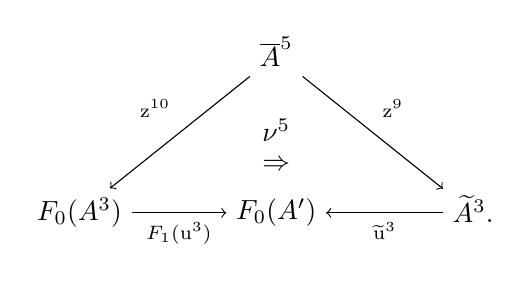
\begin{tikzpicture}[xscale=2.5,yscale=-1.0]
    \twocolorsdiagonal{mypaleorange}{white}{(0, 2) -- (1, 0) -- (2, 2) -- cycle}
    
    \node (A0_1) at (2, 2) {$\widetilde{A}^3_{\CATB}$.};
    \node (A1_0) at (1, 0) {$\overline{A}^5_{\CATB}$};
    \node (A1_2) at (1, 2) {$\functor{F}_0(A'_{\CATA})$};
    \node (A2_1) at (0, 2) {$\functor{F}_0(A^3_{\CATA})$};
    
    \node (A1_1) at (1, 1) {$\nu^5_{\CATB}$};
    \node (B1_1) at (1, 1.4) {$\Rightarrow$};
    
    \path (A1_0) edge [->]node [auto] {$\scriptstyle{\operatorname{z}^9_{\CATB}}$} (A0_1);
    \path (A1_0) edge [->]node [auto,swap] {$\scriptstyle{\operatorname{z}^{10}_{\CATB}}$} (A2_1);
    \path (A0_1) edge [->]node [auto]
      {$\scriptstyle{\widetilde{\operatorname{u}}^3_{\CATB}}$} (A1_2);
    \path (A2_1) edge [->]node [auto,swap]
      {$\scriptstyle{\functor{F}_1(\operatorname{u}^3_{\CATA})}$} (A1_2);
\end{tikzpicture}
\]

Using (BF4a) and (BF4b) for $(\CATB,\SETWBsat)$,
there are an object $\overline{A}^6_{\CATB}$, a morphism $\operatorname{z}^{11}_{\CATB}:
\overline{A}^6_{\CATB}\rightarrow\overline{A}^5_{\CATB}$ in $\SETWBsat$ and an invertible
$2$-morphism

\[
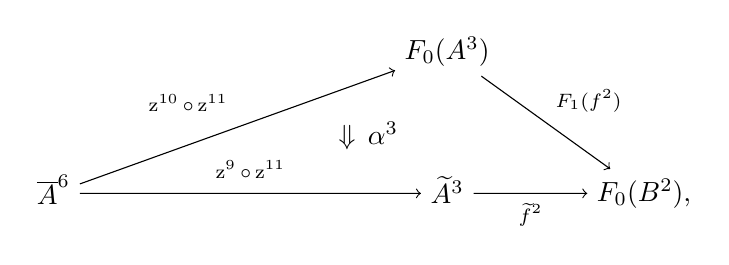
\begin{tikzpicture}[xscale=2.5,yscale=-1.8]
    \fillonecolor{mypaleorange}{(1, 2) -- (3, 1)  --  (4, 2) -- cycle}

    \node (A1_1) at (1, 2) {$\overline{A}^6_{\CATB}$};
    \node (A2_3) at (3, 2) {$\widetilde{A}^3_{\CATB}$};
    \node (A2_4) at (4, 2) {$\functor{F}_0(B^2_{\CATA})$,};
    \node (A0_3) at (3, 1) {$\functor{F}_0(A^3_{\CATA})$};
    
    \node (A1_3) at (2.6, 1.6) {$\Downarrow\,\alpha^3_{\CATB}$};

    \path (A1_1) edge [->]node [auto] {$\scriptstyle{\operatorname{z}^{10}_{\CATB}\circ
      \operatorname{z}^{11}_{\CATB}}$} (A0_3);
    \path (A1_1) edge [->]node [auto] {$\scriptstyle{\operatorname{z}^9_{\CATB}
      \circ\operatorname{z}^{11}_{\CATB}}$} (A2_3);
    \path (A2_3) edge [->]node [auto,swap] {$\scriptstyle{\widetilde{f}^2_{\CATB}}$} (A2_4);
    \path (A0_3) edge [->]node [auto] {$\scriptstyle{\functor{F}_1(f^2_{\CATA})}$} (A2_4);
\end{tikzpicture}
\]
%
such that $i_{\functor{F}_1(\operatorname{v}_{\CATA}\circ\operatorname{v}^1_{\CATA})}\ast
\alpha^3_{\CATB}$ coincides with the following composition:

\begin{equation}\label{eq-137}
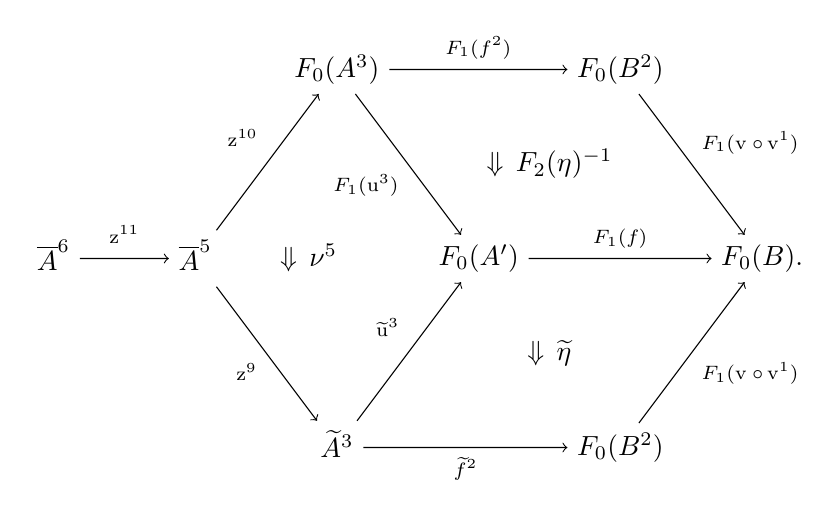
\begin{tikzpicture}[xscale=1.8, yscale=1.2]
    
    \twocolorsdiagonal{white}{mypaleorange}{(2, 3) -- (3, 5) --  (4, 3) -- (3, 1) -- cycle}

    \twocolorsdiagonal{mypaleyellow}{mypaleorange}{(3, 1) --  (5, 1) -- (6,3)  --  (4, 3) -- cycle}
  
    \twocolorsdiagonal{mypaleteal}{mypaleorange}{(3, 5) --  (5, 5) -- (6, 3)  --  (4, 3) -- cycle}
      
    \node (A1_2) at (3, 1) {$\widetilde{A}^3_{\CATB}$};
    \node (A1_5) at (5, 1) {$\functor{F}_0(B^2_{\CATA})$};
    \node (A3_0) at (1, 3) {$\overline{A}^6_{\CATB}$};
    \node (A3_1) at (2, 3) {$\overline{A}^5_{\CATB}$};
    \node (A3_4) at (4, 3) {$\functor{F}_0(A'_{\CATA})$};
    \node (A3_6) at (6, 3) {$\functor{F}_0(B_{\CATA})$.};
    \node (A5_2) at (3, 5) {$\functor{F}_0(A^3_{\CATA})$};
    \node (A5_5) at (5, 5) {$\functor{F}_0(B^2_{\CATA})$};

    \node (A3_2) at (2.8, 3) {$\Downarrow\,\nu^5_{\CATB}$};
    \node (A4_5) at (4.5, 4) {$\Downarrow\,\functor{F}_2(\eta_{\CATA})^{-1}$};
    \node (A2_5) at (4.5, 2) {$\Downarrow\,\widetilde{\eta}_{\CATB}$};
    
    \path (A5_2) edge [->]node [auto,swap]
      {$\scriptstyle{\functor{F}_1(\operatorname{u}^3_{\CATA})}$} (A3_4);
    \path (A3_0) edge [->]node [auto] {$\scriptstyle{\operatorname{z}^{11}_{\CATB}}$} (A3_1);
    \path (A5_2) edge [->]node [auto] {$\scriptstyle{\functor{F}_1(f^2_{\CATA})}$} (A5_5);
    \path (A3_1) edge [->]node [auto] {$\scriptstyle{\operatorname{z}^{10}_{\CATB}}$} (A5_2);
    \path (A3_4) edge [->]node [auto] {$\scriptstyle{\functor{F}_1(f_{\CATA})}$} (A3_6);
    \path (A3_1) edge [->]node [auto,swap] {$\scriptstyle{\operatorname{z}^9_{\CATB}}$} (A1_2);
    \path (A1_2) edge [->]node [auto]
      {$\scriptstyle{\widetilde{\operatorname{u}}^3_{\CATB}}$} (A3_4);
    \path (A5_5) edge [->]node [auto]
      {$\scriptstyle{\functor{F}_1(\operatorname{v}_{\CATA}\circ\operatorname{v}^1_{\CATA})}$} (A3_6);
    \path (A1_5) edge [->]node [auto,swap] {$\scriptstyle{\functor{F}_1(\operatorname{v}_{\CATA}
      \circ\operatorname{v}^1_{\CATA})}$} (A3_6);
    \path (A1_2) edge [->]node [auto,swap] {$\scriptstyle{\widetilde{f}^2_{\CATB}}$} (A1_5);
\end{tikzpicture}
\end{equation}

So using Lemma~\ref{lem-01} for the pair $(\underline{f}_{\CATA},\underline{h}_{\CATA}\circ
\underline{g}_{\CATA})$, we get that $G^2_{\CATB}$ is represented by the data in the following
diagram:

\begin{equation}\label{eq-195}
\begin{tikzpicture}[xscale=2.8,yscale=1.5]
    \colorvertical{mypaleorange}{(2,4) -- (4,2)  --  (2,0) -- cycle}
    \colorhorizontal{mypaleorange}{(2,4) -- (0,2)  --  (2,0) -- cycle}
      
    \node (A0_2) at (2, 0) {$\widetilde{A}^3_{\CATB}$};
    \node (A2_2) at (2, 2) {$\overline{A}^6_{\CATB}$};
    \node (A2_4) at (4, 2) {$\functor{F}_0(D_{\CATA})$.};
    \node (A2_0) at (0, 2) {$\functor{F}_0(A_{\CATA})$};
    \node (A4_2) at (2, 4) {$\functor{F}_0(A^3_{\CATA})$};
 
    \node (A2_3) at (2.8, 2) {$\Downarrow\,i_{\functor{F}_1(h_{\CATA}\circ g^1_{\CATA})}
      \ast\alpha^3_{\CATB}$};
    \node (A2_1) at (1.1, 2) {$\Downarrow\,i_{\functor{F}_1(\operatorname{u}_{\CATA})}\ast
      \nu^5_{\CATB}\ast i_{\operatorname{z}^{11}_{\CATB}}$};
 
    \path (A4_2) edge [->]node [auto]
       {$\scriptstyle{\functor{F}_1(h_{\CATA}\circ g^1_{\CATA}\circ f^2_{\CATA})}$} (A2_4);
    \path (A0_2) edge [->]node [auto,swap]
      {$\scriptstyle{\functor{F}_1(h_{\CATA}\circ g^1_{\CATA})\circ\widetilde{f}^2_{\CATB}}$} (A2_4);
    \path (A4_2) edge [->]node [auto,swap] {$\scriptstyle{\functor{F}_1(\operatorname{u}_{\CATA}
      \circ\operatorname{u}^3_{\CATA})}$} (A2_0);
    \path (A0_2) edge [->]node [auto] {$\scriptstyle{\functor{F}_1(\operatorname{u}_{\CATA})
      \circ\widetilde{\operatorname{u}}^3_{\CATB}}$} (A2_0);
    \path (A2_2) edge [->]node [auto] {$\scriptstyle{\operatorname{z}^9_{\CATB}
      \circ\operatorname{z}^{11}_{\CATB}}$} (A0_2);
    \path (A2_2) edge [->]node [auto,swap] {$\scriptstyle{\operatorname{z}^{10}_{\CATB}\circ
      \operatorname{z}^{11}_{\CATB}}$} (A4_2);
\end{tikzpicture}
\end{equation}

Now we compute $G^3_{\CATB}$: using Proposition~\ref{prop-01}  and the fact that
$\functor{F}$ is strict, there is a set of data $(A^4_{\CATA},\operatorname{u}^4_{\CATA},
\operatorname{u}^5_{\CATA},\gamma_{\CATA},\omega_{\CATA},
\rho_{\CATA})$ as in (\hyperref[F1]{F1}) - (\hyperref[F3]{F3}), such
that $\Thetaa{\underline{h}_{\CATA}}{\underline{g}_{\CATA}}{\underline{f}_{\CATA}}$ is
represented by diagram \eqref{eq-101}, so $G^3_{\CATB}$ is represented by the following diagram:

\begin{equation}\label{eq-196}
\begin{tikzpicture}[xscale=2.8,yscale=-1.5]
    \colorvertical{mypalered}{(2,4) -- (4,2)  --  (2,0) -- cycle}
    \colorhorizontal{mypalered}{(2,4) -- (0,2)  --  (2,0) -- cycle}
       
    \node (A0_2) at (2, 0) {$\functor{F}_0(A^2_{\CATA})$};
    \node (A2_2) at (2, 2) {$\functor{F}_0(A^4_{\CATA})$};
    \node (A2_4) at (4, 2) {$\functor{F}_0(D_{\CATA})$.};
    \node (A2_0) at (0, 2) {$\functor{F}_0(A_{\CATA})$};
    \node (A4_2) at (2, 4) {$\functor{F}_0(A^3_{\CATA})$};
    
    \node (A2_3) at (2.9, 2) {$\Downarrow\,i_{\functor{F}_1(h_{\CATA})}
      \ast\functor{F}_2(\rho_{\CATA})$};
    \node (A2_1) at (1.1, 2) {$\Downarrow\,i_{\functor{F}_1(\operatorname{u}_{\CATA})}
      \ast\functor{F}_2(\gamma_{\CATA})$};
    
    \path (A4_2) edge [->]node [auto,swap] {$\scriptstyle{\functor{F}_1(h_{\CATA}\circ g^1_{\CATA}
     \circ f^2_{\CATA})}$} (A2_4);
    \path (A0_2) edge [->]node [auto] {$\scriptstyle{\functor{F}_1
      (h_{\CATA}\circ l_{\CATA})}$} (A2_4);
    \path (A4_2) edge [->]node [auto]
      {$\scriptstyle{\functor{F}_1(\operatorname{u}_{\CATA}\circ\operatorname{u}^3_{\CATA})}$} (A2_0);
    \path (A0_2) edge [->]node [auto,swap] {$\scriptstyle{\functor{F}_1(\operatorname{u}_{\CATA}\circ
      \operatorname{u}^1_{\CATA}\circ\operatorname{u}^2_{\CATA})}$} (A2_0);
    \path (A2_2) edge [->]node [auto,swap] {$\scriptstyle{\functor{F}_1
      (\operatorname{u}^4_{\CATA})}$} (A0_2);
    \path (A2_2) edge [->]node [auto] {$\scriptstyle{\functor{F}_1
      (\operatorname{u}^5_{\CATA})}$} (A4_2);
\end{tikzpicture}
\end{equation}

Now we compute $G^4_{\CATB}$. In order to do that, we use (BF3) for $(\CATB,\SETWBsat)$
in order to get data as in upper part of the following diagram, with
$\operatorname{z}^{13}_{\CATB}$ in $\SETWBsat$ and $\nu^6_{\CATB}$ invertible:

\[
\begin{tikzpicture}[xscale=2.4,yscale=-1.0]
    \twocolorsdiagonal{mypalegreen}{white}{(0, 2) -- (1, 0) -- (2, 2) -- cycle}
    
    \node (A0_1) at (2, 2) {$\functor{F}_0(A^2_{\CATA})$.};
    \node (A1_0) at (1, 0) {$\overline{A}^7_{\CATB}$};
    \node (A1_2) at (1, 2) {$\functor{F}_0(A^1_{\CATA})$};
    \node (A2_1) at (0, 2) {$\widetilde{A}^2_{\CATB}$};
    
    \node (A1_1) at (1, 1) {$\nu^6_{\CATB}$};
    \node (A1_1) at (1, 1.35) {$\Rightarrow$};
    
    \path (A1_0) edge [->]node [auto] {$\scriptstyle{\operatorname{z}^{12}_{\CATB}}$} (A0_1);
    \path (A1_0) edge [->]node [auto,swap] {$\scriptstyle{\operatorname{z}^{13}_{\CATB}}$} (A2_1);
    \path (A0_1) edge [->]node [auto]
      {$\scriptstyle{\functor{F}_1(\operatorname{u}^2_{\CATA})}$} (A1_2);
    \path (A2_1) edge [->]node [auto,swap]
      {$\scriptstyle{\widetilde{\operatorname{u}}^2_{\CATB}}$} (A1_2);
\end{tikzpicture}
\]

Using (BF4a) and (BF4b) for $(\CATB,\SETWBsat)$,
we get an object $\overline{A}^8_{\CATB}$, a morphism $\operatorname{z}^{14}_{\CATB}:
\overline{A}^8_{\CATB}\rightarrow\overline{A}^7_{\CATB}$ in $\SETWBsat$ and an invertible
$2$-morphism

\[\alpha^4_{\CATB}:\,\widetilde{l}_{\CATB}\circ\operatorname{z}^{13}_{\CATB}\circ
\operatorname{z}^{14}_{\CATB}\Longrightarrow\functor{F}_1(l_{\CATA})\circ
\operatorname{z}^{12}_{\CATB}\circ\operatorname{z}^{14}_{\CATB},\]
%
such that $i_{\functor{F}_1(\operatorname{w}_{\CATA})}\ast\alpha^4_{\CATB}$ coincides with the
following composition:

\begin{equation}\label{eq-126}
\begin{tikzpicture}[xscale=1.8, yscale=-1.2]
  
    \twocolorsdiagonal{white}{mypalegreen}{(2, 3) -- (3, 1)  --  (4, 3) -- (3, 5) -- cycle}
      
    \twocolorsdiagonal{mypaleblue}{mypalegreen}{(3, 1) -- (5, 1) --  (6, 3) -- (4, 3) -- cycle}
    
    \twocolorsdiagonal{mypalemagenta}{mypalegreen}{(3, 5) -- (5, 5)  --  (6, 3) -- (4, 3) -- cycle}
    
    \node (A1_2) at (3, 1) {$\widetilde{A}^2_{\CATB}$};
    \node (A1_5) at (5, 1) {$\functor{F}_0(C'_{\CATA})$};
    \node (A3_0) at (1, 3) {$\overline{A}^8_{\CATB}$};
    \node (A3_1) at (2, 3) {$\overline{A}^7_{\CATB}$};
    \node (A3_4) at (4, 3) {$\functor{F}_0(A^1_{\CATA})$};
    \node (A3_6) at (6, 3) {$\functor{F}_0(C_{\CATA})$.};
    \node (A5_2) at (3, 5) {$\functor{F}_0(A^2_{\CATA})$};
    \node (A5_5) at (5, 5) {$\functor{F}_0(C'_{\CATA})$};

    \node (A4_5) at (4.5, 4) {$\Downarrow\,\functor{F}_2(\sigma_{\CATA})$};
    \node (A3_2) at (2.8, 3) {$\Downarrow\,\nu^6_{\CATB}$};
    \node (A2_5) at (4.5, 2) {$\Downarrow\,\widetilde{\sigma}_{\CATB}^{-1}$};

    \path (A5_2) edge [->]node [auto]
      {$\scriptstyle{\functor{F}_1(\operatorname{u}^2_{\CATA})}$} (A3_4);
    \path (A3_0) edge [->]node [auto] {$\scriptstyle{\operatorname{z}^{14}_{\CATB}}$} (A3_1);
    \path (A5_2) edge [->]node [auto,swap] {$\scriptstyle{\functor{F}_1(l_{\CATA})}$} (A5_5);
    \path (A3_1) edge [->]node [auto,swap] {$\scriptstyle{\operatorname{z}^{12}_{\CATB}}$} (A5_2);
    \path (A3_4) edge [->]node [auto] {$\scriptstyle{\functor{F}_1(g_{\CATA}
      \circ f^1_{\CATA})}$} (A3_6);
    \path (A3_1) edge [->]node [auto] {$\scriptstyle{\operatorname{z}^{13}_{\CATB}}$} (A1_2);
    \path (A1_2) edge [->]node [auto,swap]
      {$\scriptstyle{\widetilde{\operatorname{u}}^2_{\CATB}}$} (A3_4);
    \path (A5_5) edge [->]node [auto,swap]
      {$\scriptstyle{\functor{F}_1(\operatorname{w}_{\CATA})}$} (A3_6);
    \path (A1_5) edge [->]node [auto]
      {$\scriptstyle{\functor{F}_1(\operatorname{w}_{\CATA})}$} (A3_6);
    \path (A1_2) edge [->]node [auto] {$\scriptstyle{\widetilde{l}_{\CATB}}$} (A1_5);
\end{tikzpicture}
\end{equation}

Then $G^4_{\CATB}$ is represented by the following diagram:

\begin{equation}\label{eq-197}
\begin{tikzpicture}[xscale=2.8,yscale=-1.5]
    \colorvertical{mypalegreen}{(2,4) -- (4,2)  --  (2,0) -- cycle}
    \colorhorizontal{mypalegreen}{(2,4) -- (0,2)  --  (2,0) -- cycle}

    \node (A0_2) at (2, 0) {$\widetilde{A}^2_{\CATB}$};
    \node (A2_2) at (2, 2) {$\overline{A}^8_{\CATB}$};
    \node (A2_4) at (4, 2) {$\functor{F}_0(D_{\CATA})$.};
    \node (A2_0) at (0, 2) {$\functor{F}_0(A_{\CATA})$};
    \node (A4_2) at (2, 4) {$\functor{F}_0(A^2_{\CATA})$};
    
    \node (A2_3) at (2.8, 2) {$\Downarrow\,i_{\functor{F}_1(h_{\CATA})}\ast\alpha^4_{\CATB}$};
    \node (A2_1) at (1.1, 2) {$\Downarrow\,i_{\functor{F}_1(\operatorname{u}_{\CATA}
      \circ\operatorname{u}^1_{\CATA})}\ast\nu^6_{\CATB}\ast
      i_{\operatorname{z}^{14}_{\CATB}}$};
    
    \path (A4_2) edge [->]node [auto,swap]
      {$\scriptstyle{\functor{F}_1(h_{\CATA}\circ l_{\CATA})}$} (A2_4);
    \path (A0_2) edge [->]node [auto] {$\scriptstyle{\functor{F}_1
      (h_{\CATA})\circ\widetilde{l}_{\CATB}}$} (A2_4);
    \path (A4_2) edge [->]node [auto]
      {$\scriptstyle{\functor{F}_1(\operatorname{u}_{\CATA}\circ\operatorname{u}^1_{\CATA}
      \circ\operatorname{u}^2_{\CATA})}$} (A2_0);
    \path (A0_2) edge [->]node [auto,swap] {$\scriptstyle{\functor{F}_1(\operatorname{u}_{\CATA}\circ
      \operatorname{u}^1_{\CATA})\circ\widetilde{\operatorname{u}}^2_{\CATB}}$} (A2_0);
    \path (A2_2) edge [->]node [auto,swap] {$\scriptstyle{\operatorname{z}^{13}_{\CATB}
      \circ\operatorname{z}^{14}_{\CATB}}$} (A0_2);
    \path (A2_2) edge [->]node [auto] {$\scriptstyle{\operatorname{z}^{12}_{\CATB}
      \circ\operatorname{z}^{14}_{\CATB}}$} (A4_2);
\end{tikzpicture}
\end{equation}

Lastly, we compute $G^5_{\CATB}$. In order to do that, we use (BF3) for $(\CATB,\SETWBsat)$
in order to get data as in the upper part of the diagram below, with
$\operatorname{z}^{16}_{\CATB}$ in $\SETWBsat$ and $\nu^7_{\CATB}$ invertible:

\[
\begin{tikzpicture}[xscale=2.4,yscale=-1.1]
    \twocolorsdiagonal{mypalebrown}{white}{(0, 2) -- (1, 0) -- (2, 2) -- cycle}
    
    \node (A0_1) at (2, 2) {$\functor{F}_0(A^1_{\CATA})$.};
    \node (A1_0) at (1, 0) {$\overline{A}^9_{\CATB}$};
    \node (A1_2) at (1, 2) {$\functor{F}_0(A'_{\CATA})$};
    \node (A2_1) at (0, 2) {$A^1_{\CATB}$};
    
    \node (A1_1) at (1, 1) {$\nu^7_{\CATB}$};
    \node (B1_1) at (1, 1.35) {$\Rightarrow$};
    
    \path (A1_0) edge [->]node [auto] {$\scriptstyle{\operatorname{z}^{15}_{\CATB}}$} (A0_1);
    \path (A1_0) edge [->]node [auto,swap] {$\scriptstyle{\operatorname{z}^{16}_{\CATB}}$} (A2_1);
    \path (A0_1) edge [->]node [auto] {$\scriptstyle{\functor{F}_1
      (\operatorname{u}^1_{\CATA})}$} (A1_2);
    \path (A2_1) edge [->]node [auto,swap] {$\scriptstyle{\operatorname{u}^1_{\CATB}}$} (A1_2);
\end{tikzpicture}
\]

Then we use (BF4a) and (BF4b) for $(\CATB,\SETWBsat)$
in order to get an object $\overline{A}^{10}_{\CATB}$, a morphism $\operatorname{z}^{17}_{\CATB}:
\overline{A}^{10}_{\CATB} \rightarrow\overline{A}^9_{\CATB}$ in $\SETWBsat$ and an invertible
$2$-morphism

\[\varepsilon_{\CATB}:\,f^1_{\CATB}\circ\operatorname{z}^{16}_{\CATB}\circ
\operatorname{z}^{17}_{\CATB}\Longrightarrow\functor{F}_1(f^1_{\CATA})\circ
\operatorname{z}^{15}_{\CATB}\circ\operatorname{z}^{17}_{\CATB},\]
%
such that $i_{\functor{F}_1(\operatorname{v}_{\CATA})}\ast\varepsilon_{\CATB}$ coincides with the
following composition:

\begin{equation}\label{eq-128}
\begin{tikzpicture}[xscale=1.8, yscale=1.2]
  
    \twocolorsdiagonal{white}{mypalebrown}{(2, 3) -- (3, 5) -- (4, 3) -- (3, 1) -- cycle}
    \twocolorsdiagonal{mypalepink}{mypalebrown}{(3, 1) -- (5, 1) -- (6, 3) -- (4, 3) -- cycle}

    \def\formaa#1#2#3
    {\begin{scope}[shift={#1}, scale=#2]
    \draw [fill=#3, draw=white, line width=0pt, rounded corners] (3, 5) -- (5, 5)  -- (6, 3) -- (4, 3) -- cycle;  
    \end{scope}}

    \formaa{(0,0)}{1}{mypalelime}
    \formaa{(1.35,1.2)}{0.7}{white}
    
    %%%
    
    \node (A1_2) at (3, 1) {$\functor{F}_0(A^1_{\CATA})$};
    \node (A1_5) at (5, 1) {$\functor{F}_0(B'_{\CATA})$};
    \node (A3_0) at (1, 3) {$\overline{A}^{10}_{\CATB}$};
    \node (A3_1) at (2, 3) {$\overline{A}^9_{\CATB}$};
    \node (A3_4) at (4, 3) {$\functor{F}_0(A'_{\CATA})$};
    \node (A3_6) at (6, 3) {$\functor{F}_0(B_{\CATA})$.};
    \node (A5_2) at (3, 5) {$A^1_{\CATB}$};
    \node (A5_5) at (5, 5) {$\functor{F}_0(B'_{\CATA})$};
    
    \node (A2_5) at (4.5, 2) {$\Downarrow\,\functor{F}_2(\delta_{\CATA})$};
    \node (A4_5) at (4.5, 4) {$\Downarrow\,\delta_{\CATB}^{-1}$};
    \node (A3_2) at (2.8, 3) {$\Downarrow\,\nu^7_{\CATB}$};
    
    \path (A5_2) edge [->]node [auto,swap] {$\scriptstyle{\operatorname{u}^1_{\CATB}}$} (A3_4);
    \path (A3_0) edge [->]node [auto] {$\scriptstyle{\operatorname{z}^{17}_{\CATB}}$} (A3_1);
    \path (A5_2) edge [->]node [auto] {$\scriptstyle{f^1_{\CATB}}$} (A5_5);
    \path (A3_1) edge [->]node [auto] {$\scriptstyle{\operatorname{z}^{16}_{\CATB}}$} (A5_2);
    \path (A3_4) edge [->]node [auto] {$\scriptstyle{\functor{F}_1(f_{\CATA})}$} (A3_6);
    \path (A3_1) edge [->]node [auto,swap] {$\scriptstyle{\operatorname{z}^{15}_{\CATB}}$} (A1_2);
    \path (A1_2) edge [->]node [auto]
      {$\scriptstyle{\functor{F}_1(\operatorname{u}^1_{\CATA})}$} (A3_4);
    \path (A5_5) edge [->]node [auto]
      {$\scriptstyle{\functor{F}_1(\operatorname{v}_{\CATA})}$} (A3_6);
    \path (A1_5) edge [->]node [auto,swap]
      {$\scriptstyle{\functor{F}_1(\operatorname{v}_{\CATA})}$} (A3_6);
    \path (A1_2) edge [->]node [auto,swap] {$\scriptstyle{\functor{F}_1(f^1_{\CATA})}$} (A1_5);
\end{tikzpicture}
\end{equation}

Now by construction both $\operatorname{u}^1_{\CATB}$ and $\operatorname{z}^{16}_{\CATB}$ belong to
$\SETWBsat$, so by (BF2) and (BF5) applied to $(\nu^7_{\CATB})^{-1}$ we conclude that $\functor{F}_1
(\operatorname{u}^1_{\CATA})\circ\operatorname{z}^{15}_{\CATB}$ belongs to $\SETWBsat$. Moreover,
by construction also $\functor{F}_1(\operatorname{u}^1_{\CATA})$ belongs to $\SETWBsat$. Therefore,
by~\cite[Proposition~2.11(ii)]{T4} we conclude that also $\operatorname{z}^{15}_{\CATB}$ belongs to
$\SETWBsat$. So by Lemma~\ref{lem-01} we can use $(\nu^7_{\CATB})^{-1}$ and $\varepsilon_{\CATB}^{-1}$
in order to compute $\Psi_{\underline{g}_{\CATA},\underline{f}_{\CATA}}^{\functor{N}}$.
Taking the inverse, we get that $\left(\Psi_{\underline{g}_{\CATA},
\underline{f}_{\CATA}}^{\functor{N}}\right)^{-1}$ is represented
by the following diagram:

\[
\begin{tikzpicture}[xscale=2.8,yscale=-1.5]
    \node (A0_2) at (2, 0) {$A^1_{\CATB}$};
    \node (A2_2) at (2, 2) {$\overline{A}^{10}_{\CATB}$};
    \node (A2_4) at (4, 2) {$\functor{F}_0(C_{\CATA})$.};
    \node (A2_0) at (0, 2) {$\functor{F}_0(A_{\CATA})$};
    \node (A4_2) at (2, 4) {$\functor{F}_0(A^1_{\CATA})$};
    
    \node (A2_3) at (2.8, 2) {$\Downarrow\,i_{\functor{F}_1(g_{\CATA})}\ast\varepsilon_{\CATB}$};
    \node (A2_1) at (1.1, 2) {$\Downarrow\,i_{\functor{F}_1(\operatorname{u}_{\CATA})}\ast
      \nu^7_{\CATB}\ast i_{\operatorname{z}^{17}_{\CATB}}$};
    
    \path (A4_2) edge [->]node [auto,swap]
      {$\scriptstyle{\functor{F}_1(g_{\CATA}\circ f^1_{\CATA})}$} (A2_4);
    \path (A0_2) edge [->]node [auto] {$\scriptstyle{\functor{F}_1
      (g_{\CATA})\circ f^1_{\CATB}}$} (A2_4);
    \path (A4_2) edge [->]node [auto]
      {$\scriptstyle{\functor{F}_1(\operatorname{u}_{\CATA}\circ\operatorname{u}^1_{\CATA})}$} (A2_0);
    \path (A0_2) edge [->]node [auto,swap] {$\scriptstyle{\functor{F}_1(\operatorname{u}_{\CATA})
      \circ\operatorname{u}^1_{\CATB}}$} (A2_0);
    \path (A2_2) edge [->]node [auto,swap] {$\scriptstyle{\operatorname{z}^{16}_{\CATB}
      \circ\operatorname{z}^{17}_{\CATB}}$} (A0_2);
    \path (A2_2) edge [->]node [auto] {$\scriptstyle{\operatorname{z}^{15}_{\CATB}
      \circ\operatorname{z}^{17}_{\CATB}}$} (A4_2);
\end{tikzpicture}
\]

Following~\cite[Proposition~0.4]{T3}, we compute $G^5_{\CATB}$ as follows. We use (BF3)
for $(\CATB,\SETWBsat)$ in order to get data as in the upper parts of the following $2$ diagrams,
with $\operatorname{z}^{21}_{\CATB}$ and $\operatorname{z}^{19}_{\CATB}$ in
$\SETWBsat$ and $\nu^9_{\CATB}$ and $\nu^8_{\CATB}$ invertible:

\[
\begin{tikzpicture}[xscale=2.2,yscale=-1.1]
    \twocolorsdiagonal{white}{mypaleblue}{(6, 2) -- (7, 0) -- (8, 2) -- cycle}
    \twocolorsdiagonal{white}{mypaleblue}{(3, 2) -- (4, 0) -- (5, 2) -- cycle}

    \node (A0_1) at (8, 2) {$\widetilde{A}^2_{\CATB}$.};
    \node (A1_0) at (7, 0) {$\overline{A}^{11}_{\CATB}$};
    \node (A1_2) at (7, 2) {$\functor{F}_0(A^1_{\CATA})$};
    \node (A2_1) at (6, 2) {$\overline{A}^{10}_{\CATB}$};
    
    \node (A1_1) at (7, 1) {$\nu^8_{\CATB}$};
    \node (C1_1) at (7, 1.35) {$\Rightarrow$};
    
    \node (B0_1) at (5, 2) {$A^2_{\CATB}$,};
    \node (B1_0) at (4, 0) {$\overline{A}^{12}_{\CATB}$};
    \node (B1_2) at (4, 2) {$A^1_{\CATB}$};
    \node (B2_1) at (3, 2) {$\overline{A}^{10}_{\CATB}$};
    
    \node (B1_1) at (4, 1) {$\nu^9_{\CATB}$};
    \node (D1_1) at (4, 1.35) {$\Rightarrow$};
    
    \path (A1_0) edge [->]node [auto] {$\scriptstyle{\operatorname{z}^{18}_{\CATB}}$} (A0_1);
    \path (A1_0) edge [->]node [auto,swap] {$\scriptstyle{\operatorname{z}^{19}_{\CATB}}$} (A2_1);
    \path (A0_1) edge [->]node [auto]
      {$\scriptstyle{\widetilde{\operatorname{u}}^2_{\CATB}}$} (A1_2);
    \path (A2_1) edge [->]node [auto,swap]
      {$\scriptstyle{\operatorname{z}^{15}_{\CATB}\circ\operatorname{z}^{17}_{\CATB}}$} (A1_2);
      
    \path (B1_0) edge [->]node [auto] {$\scriptstyle{\operatorname{z}^{20}_{\CATB}}$} (B0_1);
    \path (B1_0) edge [->]node [auto,swap] {$\scriptstyle{\operatorname{z}^{21}_{\CATB}}$} (B2_1);
    \path (B0_1) edge [->]node [auto] {$\scriptstyle{\operatorname{u}^2_{\CATB}}$} (B1_2);
    \path (B2_1) edge [->]node [auto,swap]
      {$\scriptstyle{\operatorname{z}^{16}_{\CATB}\circ\operatorname{z}^{17}_{\CATB}}$} (B1_2);
\end{tikzpicture}
\]

Now we use again (BF3) for $(\CATB,\SETWBsat)$
in order to get data as in the upper part of the following diagram, with
$\operatorname{z}^{23}_{\CATB}$ in $\SETWBsat$ and $\nu^{10}_{\CATB}$ invertible:

\[
\begin{tikzpicture}[xscale=-2.2,yscale=-1.1]
    \twocolorsdiagonal{white}{mypaleblue}{(0, 2) -- (1, 0) -- (2, 2) -- cycle};

    \node (A0_1) at (0, 2) {$\overline{A}^{11}_{\CATB}$.};
    \node (A1_0) at (1, 0) {$\overline{A}^{13}_{\CATB}$};
    \node (A1_2) at (1, 2) {$\overline{A}^{10}_{\CATB}$};
    \node (A2_1) at (2, 2) {$\overline{A}^{12}_{\CATB}$};
    
    \node (A1_1) at (1, 1) {$\nu^{10}_{\CATB}$};
    \node (B1_1) at (1, 1.35) {$\Rightarrow$};
    
    \path (A1_0) edge [->]node [auto] {$\scriptstyle{\operatorname{z}^{22}_{\CATB}}$} (A0_1);
    \path (A1_0) edge [->]node [auto,swap] {$\scriptstyle{\operatorname{z}^{23}_{\CATB}}$} (A2_1);
    \path (A0_1) edge [->]node [auto] {$\scriptstyle{\operatorname{z}^{19}_{\CATB}}$} (A1_2);
    \path (A2_1) edge [->]node [auto,swap] {$\scriptstyle{\operatorname{z}^{21}_{\CATB}}$} (A1_2);
\end{tikzpicture}
\]

Moreover, we use (BF4a) and (BF4b) for $(\CATB,\SETWBsat)$
in order to get an object $\overline{A}^{14}_{\CATB}$,
a morphism $\operatorname{z}^{24}_{\CATB}:\overline{A}^{14}_{\CATB}\rightarrow
\overline{A}^{13}_{\CATB}$ in $\SETWBsat$ and an invertible $2$-morphism

\[\alpha^5_{\CATB}:\,l_{\CATB}\circ\operatorname{z}^{20}_{\CATB}\circ
\operatorname{z}^{23}_{\CATB}\circ\operatorname{z}^{24}_{\CATB}\Longrightarrow
\widetilde{l}_{\CATB}\circ\operatorname{z}^{18}_{\CATB}\circ
\operatorname{z}^{22}_{\CATB}\circ\operatorname{z}^{24}_{\CATB},\]
%
such that $i_{\functor{F}_1(\operatorname{w}_{\CATA})}\ast\alpha^5_{\CATB}$ coincides with the
following composition:

\begin{equation}\label{eq-127}
\begin{tikzpicture}[xscale=2.0, yscale=-1.4]
    \twocolorsdiagonal{mypaleblue}{white}{(1,3) -- (3,1) -- (4, 2) -- (3, 3) -- (4, 4) -- (3, 5) -- cycle}
    \twocolorsdiagonal{mypaleblue}{mypalegreen}{(3, 5) -- (5, 3) -- (6.2, 3) -- (4.2, 5) -- cycle}
    
    \fillonecolor{mypalebrown}{(3, 3) -- (4, 2) -- (5, 3) -- (4, 4) -- cycle}
    
    %%%
    
    \def \x {0.05*2.0/2.0}
    \def \y {0.05*2.0/1.4}
    
    \def \formaa {(3, 1) -- (4.2, 1) -- (6.2, 3) -- (5, 3) -- cycle}
    \def \formab {(3+6*\x, 1+2*\y) -- (4.2-\x, 1+2*\y) -- (6.2-6*\x, 3-2*\y) -- (5+\x, 3-2*\y) -- cycle}
    
    \fillonecolorminus{mypaleblue}{\formaa}{\formab}
    
    %%%
    
    \node (A3_5) at (5, 3) {$\functor{F}_0(B'_{\CATA})$};
    \node (A1_3) at (3, 1) {$A^2_{\CATB}$};
    \node (A1_5) at (4.2, 1) {$\functor{F}_0(C'_{\CATA})$};
    \node (A2_2) at (2, 2) {$\overline{A}^{12}_{\CATB}$};
    \node (A2_4) at (4, 2) {$A^1_{\CATB}$};
    \node (A3_0) at (0.3, 3) {$\overline{A}^{14}_{\CATB}$};
    \node (A3_1) at (1, 3) {$\overline{A}^{13}_{\CATB}$};
    \node (A3_3) at (3, 3) {$\overline{A}^{10}_{\CATB}$};
    \node (A3_6) at (6.2, 3) {$\functor{F}_0(C_{\CATA})$.};
    \node (A4_2) at (2, 4) {$\overline{A}^{11}_{\CATB}$};
    \node (A4_4) at (4, 4) {$5\functor{F}_0(A^1_{\CATA})$};
    \node (A5_3) at (3, 5) {$\widetilde{A}^2_{\CATB}$};
    \node (A5_5) at (4.2, 5) {$\functor{F}_0(C'_{\CATA})$};
     
    \node (A5_4) at (4.6, 4) {$\Downarrow\,\widetilde{\sigma}_{\CATB}$};
    \node (A2_3) at (2.7, 2) {$\Downarrow\,(\nu^9_{\CATB})^{-1}$};
    \node (A3_2) at (1.8, 3) {$\Downarrow\,\nu^{10}_{\CATB}$};
    \node (B3_5) at (3.8, 3) {$\Downarrow\,\varepsilon_{\CATB}$};
    \node (A4_3) at (2.8, 4.1) {$\Downarrow\,\nu^8_{\CATB}$};
    \node (A1_4) at (4.6, 2) {$\Downarrow\,\sigma^{-1}_{\CATB}$};
    
    \path (A5_3) edge [->]node [auto] {$\scriptstyle{\widetilde{\operatorname{u}}^2_{\CATB}}$} (A4_4);
    \path (A1_3) edge [->]node [auto] {$\scriptstyle{l_{\CATB}}$} (A1_5);
    \path (A2_2) edge [->]node [auto,swap] {$\scriptstyle{\operatorname{z}^{21}_{\CATB}}$} (A3_3);
    \path (A2_2) edge [->]node [auto] {$\scriptstyle{\operatorname{z}^{20}_{\CATB}}$} (A1_3);
    \path (A3_3) edge [->]node [auto,swap] {$\scriptstyle{\operatorname{z}^{15}_{\CATB}
      \circ\operatorname{z}^{17}_{\CATB}}$} (A4_4);
    \path (A4_2) edge [->]node [auto] {$\scriptstyle{\operatorname{z}^{19}_{\CATB}}$} (A3_3);
    \path (A3_0) edge [->]node [auto] {$\scriptstyle{\operatorname{z}^{24}_{\CATB}}$} (A3_1);
    \path (A4_2) edge [->]node [auto,swap] {$\scriptstyle{\operatorname{z}^{18}_{\CATB}}$} (A5_3);
    \path (A5_3) edge [->]node [auto,swap] {$\scriptstyle{\widetilde{l}_{\CATB}}$} (A5_5);
    \path (A2_4) edge [->]node [auto,swap] {$\scriptstyle{f^1_{\CATB}}$} (A3_5);
    \path (A3_5) edge [->]node [auto,swap] {$\scriptstyle{\functor{F}_1(g_{\CATA})}$} (A3_6);
    \path (A4_4) edge [->]node [auto] {$\scriptstyle{\functor{F}_1(f^1_{\CATA})}$} (A3_5);
    \path (A3_1) edge [->]node [auto] {$\scriptstyle{\operatorname{z}^{23}_{\CATB}}$} (A2_2);
    \path (A1_5) edge [->]node [auto]
      {$\scriptstyle{\functor{F}_1(\operatorname{w}_{\CATA})}$} (A3_6);
    \path (A1_3) edge [->]node [auto,swap] {$\scriptstyle{\operatorname{u}^2_{\CATB}}$} (A2_4);
    \path (A5_5) edge [->]node [auto,swap]
      {$\scriptstyle{\functor{F}_1(\operatorname{w}_{\CATA})}$} (A3_6);
    \path (A3_1) edge [->]node [auto,swap] {$\scriptstyle{\operatorname{z}^{22}_{\CATB}}$} (A4_2);
    \path (A3_3) edge [->]node [auto] {$\scriptstyle{\operatorname{z}^{16}_{\CATB}
      \circ\operatorname{z}^{17}_{\CATB}}$} (A2_4);
\end{tikzpicture}
\end{equation}

Then by~\cite[Proposition~0.4]{T3} $G^5_{\CATB}$ is represented by the following diagram

\begin{equation}\label{eq-198}
\begin{tikzpicture}[xscale=2.8,yscale=-1.5]
    \colorvertical{mypaleblue}{(2,4) -- (4,2)  --  (2,0) -- cycle}
    \colorhorizontal{mypaleblue}{(2,4) -- (0,2)  --  (2,0) -- cycle}

    \node (A0_2) at (2, 0) {$A^2_{\CATB}$};
    \node (A2_2) at (2, 2) {$\overline{A}^{14}_{\CATB}$};
    \node (A2_4) at (4, 2) {$\functor{F}_0(D_{\CATA})$,};
    \node (A2_0) at (0, 2) {$\functor{F}_0(A_{\CATA})$};
    \node (A4_2) at (2, 4) {$\widetilde{A}^2_{\CATB}$};
    
    \node (A2_3) at (2.8, 2) {$\Downarrow\,i_{\functor{F}_1(h_{\CATA})}\ast\alpha^5_{\CATB}$};
    \node (A2_1) at (1.1, 2) {$\Downarrow\,i_{\functor{F}_1
      (\operatorname{u}_{\CATA})}\ast\tau_{\CATB}\ast i_{\operatorname{z}^{24}_{\CATB}}$};
    
    \path (A4_2) edge [->]node [auto,swap] {$\scriptstyle{\functor{F}_1
      (h_{\CATA})\circ\widetilde{l}_{\CATB}}$} (A2_4);
    \path (A0_2) edge [->]node [auto] {$\scriptstyle{\functor{F}_1
      (h_{\CATA})\circ l_{\CATB}}$} (A2_4);
    \path (A4_2) edge [->]node [auto]
      {$\scriptstyle{\functor{F}_1(\operatorname{u}_{\CATA}\circ
      \operatorname{u}^1_{\CATA})\circ\widetilde{\operatorname{u}}^2_{\CATB}}$} (A2_0);
    \path (A0_2) edge [->]node [auto,swap] {$\scriptstyle{\functor{F}_1(\operatorname{u}_{\CATA})\circ
      \operatorname{u}^1_{\CATB}\circ\operatorname{u}^2_{\CATB}}$} (A2_0);
    \path (A2_2) edge [->]node [auto,swap] {$\scriptstyle{\operatorname{z}^{20}_{\CATB}
      \circ\operatorname{z}^{23}_{\CATB}\circ\operatorname{z}^{24}_{\CATB}}$} (A0_2);
    \path (A2_2) edge [->]node [auto] {$\scriptstyle{\operatorname{z}^{18}_{\CATB}
      \circ\operatorname{z}^{22}_{\CATB}\circ\operatorname{z}^{24}_{\CATB}}$} (A4_2);
\end{tikzpicture}
\end{equation}
%
where $\tau_{\CATB}$ is the following composition:

\[
\begin{tikzpicture}[xscale=2.8, yscale=-1.2]
    \twocolorsdiagonal{mypaleblue}{white}{(1, -3) -- (3, -3) -- (4, -1) -- (3, -1) -- 
      (3, 0) -- (2, -1) -- (1.5, -2) -- cycle}
    \twocolorsdiagonal{mypalebrown}{white}{(3, -1) -- (4, -1) -- (4, 2) -- (3, 0) -- cycle}
    
    \node (C2_2) at (1, -3) {$\overline{A}^{13}_{\CATB}$};
    \node (C3_3) at (2, -3) {$\overline{A}^{12}_{\CATB}$};
    \node (C4_4) at (1.5, -2) {$\overline{A}^{11}_{\CATB}$};
    \node (C5_5) at (2.5, -2) {$\overline{A}^{10}_{\CATB}$};
    \node (C6_6) at (3, -3) {$A^2_{\CATB}$};
    \node (C7_7) at (3, -1) {$\overline{A}^9_{\CATB}$};
    \node (C8_8) at (4, -1) {$A^1_{\CATB}$};
    \node (B3_3) at (2, -1) {$\widetilde{A}^2_{\CATB}$};
    \node (A0_3) at (3, 0) {$\functor{F}_0(A^1_{\CATA})$};
    \node (A2_4) at (4, 2) {$\functor{F}_0(A'_{\CATA})$};

    \node (D2_2) at (3.5, 0) {$\Downarrow\,\nu^7_{\CATB}$};
    \node (D3_3) at (1.7, -2.5) {$\Downarrow\,\nu^{10}_{\CATB}$};
    \node (D4_4) at (2.4, -1.3) {$\Downarrow\,\nu^8_{\CATB}$};
    \node (D5_5) at (3, -2.2) {$\Downarrow\,(\nu^9_{\CATB})^{-1}$};

    \path (C2_2) edge [->]node [auto] {$\scriptstyle{\operatorname{z}^{23}_{\CATB}}$} (C3_3);
    \path (C2_2) edge [->]node [auto,swap] {$\scriptstyle{\operatorname{z}^{22}_{\CATB}}$} (C4_4);
    \path (C4_4) edge [->]node [auto,swap]
      {$\scriptstyle{\operatorname{z}^{19}_{\CATB}}$} (C5_5);
    \path (C3_3) edge [->]node [auto]
      {$\scriptstyle{\operatorname{z}^{21}_{\CATB}}$} (C5_5);
    \path (C4_4) edge [->]node [auto,swap]
      {$\scriptstyle{\operatorname{z}^{18}_{\CATB}}$} (B3_3);
    \path (C5_5) edge [->]node [auto]
      {$\scriptstyle{\operatorname{z}^{17}_{\CATB}}$} (C7_7);
    \path (C7_7) edge [->]node [auto,swap]
      {$\scriptstyle{\operatorname{z}^{16}_{\CATB}}$} (C8_8);
    \path (C7_7) edge [->]node [auto,swap]
      {$\scriptstyle{\operatorname{z}^{15}_{\CATB}}$} (A0_3);
    \path (C3_3) edge [->]node [auto]
      {$\scriptstyle{\operatorname{z}^{20}_{\CATB}}$} (C6_6);
    \path (C6_6) edge [->]node [auto]
      {$\scriptstyle{\operatorname{u}^2_{\CATB}}$} (C8_8);
    \path (C8_8) edge [->]node [auto]
      {$\scriptstyle{\operatorname{u}^1_{\CATB}}$} (A2_4);
    \path (A0_3) edge [->]node [auto,swap]
      {$\scriptstyle{\functor{F}_1(\operatorname{u}^1_{\CATA})}$} (A2_4);
    \path (B3_3) edge [->]node [auto,swap]
      {$\scriptstyle{\widetilde{\operatorname{u}}^2_{\CATB}}$} (A0_3);
    \end{tikzpicture}
\]

Now we have to compose vertically all the $2$-morphisms $G^1_{\CATB},\cdots,G^5_{\CATB}$ obtained so
far. We start by computing $G^1_{\CATB}\odot G^2_{\CATB}$ using \eqref{eq-194} and \eqref{eq-195}.
First of all, we use (BF3) for $(\CATB,\SETWBsat)$ in order to get data as in the upper part of
the following diagram, with
$\operatorname{z}^{26}_{\CATB}$ in $\SETWBsat$ and $\nu^{11}_{\CATB}$ invertible:

\[
\begin{tikzpicture}[xscale=2.5,yscale=-1.0]
    \twocolorsdiagonal{mypalecyan}{white}{(0,2) -- (1,0)  --  (2,2) -- cycle}

    \node (A0_1) at (2, 2) {$\overline{A}^4_{\CATB}$.};
    \node (A1_0) at (1, 0) {$\overline{A}^{15}_{\CATB}$};
    \node (A1_2) at (1, 2) {$\widetilde{A}^3_{\CATB}$};
    \node (A2_1) at (0, 2) {$\overline{A}^6_{\CATB}$};
    
    \node (A1_1) at (1, 1) {$\nu^{11}_{\CATB}$};
    \node (A1_1) at (1, 1.4) {$\Rightarrow$};
    
    \path (A1_0) edge [->]node [auto] {$\scriptstyle{\operatorname{z}^{25}_{\CATB}}$} (A0_1);
    \path (A1_0) edge [->]node [auto,swap] {$\scriptstyle{\operatorname{z}^{26}_{\CATB}}$} (A2_1);
    \path (A0_1) edge [->]node [auto] {$\scriptstyle{\operatorname{z}^4_{\CATB}\circ
      \operatorname{z}^6_{\CATB}\circ\operatorname{z}^8_{\CATB}}$} (A1_2);
    \path (A2_1) edge [->]node [auto,swap] {$\scriptstyle{\operatorname{z}^9_{\CATB}
      \circ\operatorname{z}^{11}_{\CATB}}$} (A1_2);
\end{tikzpicture}
\]

Then by~\cite[Proposition~0.2]{T3}, $G^1_{\CATB}\odot G^2_{\CATB}$ is represented by the
following diagram

\begin{equation}\label{eq-199}
\begin{tikzpicture}[xscale=2.8,yscale=-1.5]
    \colorhorizontal{mypaleorange}{(2,0) -- (2,2)  --  (0,2) -- cycle}
    \colorhorizontal{mypaleyellow}{(2,2) -- (2,4)  --  (0,2) -- cycle}

    \colorvertical{mypaleorange}{(2,0) -- (2,2)  --  (4,2) -- cycle}
    \colorvertical{mypaleyellow}{(2,2) -- (2,4)  --  (4,2) -- cycle}
   
    \node (A0_2) at (2, 0) {$\functor{F}_0(A^3_{\CATB})$};
    \node (A2_2) at (2, 2) {$\overline{A}^{15}_{\CATB}$};
    \node (A2_4) at (4, 2) {$\functor{F}_0(D_{\CATA})$,};
    \node (A2_0) at (0, 2) {$\functor{F}_0(A_{\CATA})$};
    \node (A4_2) at (2, 4) {$A^3_{\CATB}$};
    
    \node (A2_3) at (2.8, 2) {$\Downarrow\,i_{\functor{F}_1(h_{\CATA})}\ast\psi^1_{\CATB}$};
    \node (A2_1) at (1.1, 2)
      {$\Downarrow\,i_{\functor{F}_1(\operatorname{u}_{\CATA})}\ast\phi^1_{\CATB}$};

    \path (A4_2) edge [->]node [auto,swap]
      {$\scriptstyle{\functor{F}_1(h_{\CATA})\circ g^1_{\CATB}\circ f^2_{\CATB}}$} (A2_4);
    \path (A0_2) edge [->]node [auto] {$\scriptstyle{\functor{F}_1
      (h_{\CATA}\circ g^1_{\CATA}\circ f^2_{\CATA})}$} (A2_4);
    \path (A4_2) edge [->]node [auto]
      {$\scriptstyle{\functor{F}_1(\operatorname{u}_{\CATA})\circ\operatorname{u}^3_{\CATB}}$} (A2_0);
    \path (A0_2) edge [->]node [auto,swap] {$\scriptstyle{\functor{F}_1(\operatorname{u}_{\CATA}
      \circ\operatorname{u}^3_{\CATA})}$} (A2_0);
    \path (A2_2) edge [->]node [auto,swap] {$\scriptstyle{\operatorname{z}^{10}_{\CATB}
      \circ\operatorname{z}^{11}_{\CATB}\circ\operatorname{z}^{26}_{\CATB}}$} (A0_2);
    \path (A2_2) edge [->]node [auto] {$\scriptstyle{\operatorname{z}^5_{\CATB}
      \circ\operatorname{z}^7_{\CATB}\circ\operatorname{z}^8_{\CATB}
      \circ\operatorname{z}^{25}_{\CATB}}$} (A4_2);
\end{tikzpicture}
\end{equation}
%
where $\phi^1_{\CATB}$ is the following composition:

\[
\begin{tikzpicture}[xscale=1.8,yscale=-1.2]
    \twocolorsdiagonal{mypaleorange}{white}{(3,1) -- (5,1)  --  (6,3) -- (4,3) -- cycle}
    \twocolorsdiagonal{mypaleyellow}{white}{(3,5) -- (5,5)  --  (6,3) -- (4,3) -- cycle}
    \twocolorsdiagonal{mypalecyan}{white}{(1, 3) -- (2, 1) -- (3, 1) -- (4, 3) -- (3, 5) -- (2, 5) -- cycle}
      
    \node (A1_2) at (3, 1) {$\overline{A}^5_{\CATB}$};
    \node (B1_2) at (2, 1) {$\overline{A}^6_{\CATB}$};
    \node (A1_5) at (5, 1) {$\functor{F}_0(A^3_{\CATA})$};
    \node (A3_1) at (1, 3) {$\overline{A}^{15}_{\CATB}$};
    \node (A3_4) at (4, 3) {$\widetilde{A}^3_{\CATB}$};
    \node (A3_6) at (6, 3) {$\functor{F}_0(A'_{\CATA})$};
    \node (A5_2) at (2, 5) {$\overline{A}^4_{\CATB}$};
    \node (A5_5) at (5, 5) {$A^3_{\CATB}$};
    \node (B1_1) at (3, 5) {$\overline{A}^3_{\CATB}$};
    
    \node (A4_5) at (4.5, 4) {$\Downarrow\,\nu^4_{\CATB}$};
    \node (A3_2) at (2.5, 3) {$\Downarrow\,\nu^{11}_{\CATB}$};
    \node (A2_5) at (4.5, 2) {$\Downarrow\,\nu^5_{\CATB}$};
    
    \path (B1_1) edge [->]node [auto,swap] {$\scriptstyle{\operatorname{z}^5_{\CATB}
      \circ\operatorname{z}^7_{\CATB}}$} (A5_5);
    \path (A5_2) edge [->]node [auto,swap] {$\scriptstyle{\operatorname{z}^8_{\CATB}}$} (B1_1);
    \path (B1_1) edge [->]node [auto] {$\scriptstyle{\operatorname{z}^4_{\CATB}
      \circ\operatorname{z}^6_{\CATB}}$} (A3_4);
    \path (A3_1) edge [->]node [auto,swap] {$\scriptstyle{\operatorname{z}^{25}_{\CATB}}$} (A5_2);
    \path (A3_4) edge [->]node [auto] {$\scriptstyle{\widetilde{\operatorname{u}}^3_{\CATB}}$} (A3_6);
    \path (A3_1) edge [->]node [auto] {$\scriptstyle{\operatorname{z}^{26}_{\CATB}}$} (B1_2);
    \path (B1_2) edge [->]node [auto]
      {$\scriptstyle{\operatorname{z}^{11}_{\CATB}}$} (A1_2);
    \path (A1_2) edge [->]node [auto,swap]
      {$\scriptstyle{\operatorname{z}^9_{\CATB}}$} (A3_4);
    \path (A5_5) edge [->]node [auto,swap]
      {$\scriptstyle{\operatorname{u}^3_{\CATB}}$} (A3_6);
    \path (A1_5) edge [->]node [auto]
      {$\scriptstyle{\functor{F}_1(\operatorname{u}^3_{\CATA})}$} (A3_6);
    \path (A1_2) edge [->]node [auto] {$\scriptstyle{\operatorname{z}^{10}_{\CATB}}$} (A1_5);
\end{tikzpicture}
\]
%
and $\psi^1_{\CATB}$ is the following composition

\[
\begin{tikzpicture}[xscale=2.5,yscale=-1.8]
    \fillonecolor{mypaleorange}{(1, 2) -- (3, 1)  --  (4, 2) -- cycle}
    \twocolorsdiagonal{mypalecyan}{white}{(0, 2) -- (3, 2) -- (2, 3) -- (1, 3) -- cycle}
    \fillonecolor{mypaleyellow}{(1, 3) -- (3, 3) -- (2, 4) -- cycle}
    \fillonecolor{mypaleolive}{(3, 3) -- (4, 2) -- (5, 2) -- (4, 4) -- cycle}
    
    \twocolorsdiagonal{mypalelime}{mypaleyellow}{(2, 3) -- (3, 2) -- (4, 2) -- (3, 3) -- cycle}
    \twocolorsdiagonal{mypalelime}{mypaleyellow}{(2, 4) -- (3, 3) -- (4, 4) -- cycle}

    \node (A0_3) at (3, 1) {$\functor{F}_0(A^3_{\CATA})$};
    \node (A1_1) at (1, 2) {$\overline{A}^6_{\CATB}$};
    \node (A2_0) at (0, 2) {$\overline{A}^{15}_{\CATB}$};
    \node (A2_3) at (3, 2) {$\widetilde{A}^3_{\CATB}$};
    \node (A2_4) at (4, 2) {$\functor{F}_0(B^2_{\CATA})$};
    \node (A2_5) at (5, 2) {$\functor{F}_0(C'_{\CATA})$.};
    \node (A3_1) at (1, 3) {$\overline{A}^4_{\CATB}$};
    \node (A3_2) at (2, 3) {$\overline{A}^1_{\CATB}$};
    \node (A3_3) at (3, 3) {$\overline{B}^2_{\CATB}$};
    \node (A4_2) at (2, 4) {$\overline{A}^2_{\CATB}$};
    \node (A4_3) at (3, 4) {$A^3_{\CATB}$};
    \node (A4_4) at (4, 4) {$B^2_{\CATB}$};

    \node (A2_1) at (1.5, 2.5) {$\Downarrow\,\nu^{11}_{\CATB}$};
    \node (A3_4) at (4, 3) {$\Downarrow\,\alpha^1_{\CATB}$};
    \node (A4_1) at (2, 3.5) {$\Downarrow\,\alpha^2_{\CATB}$};
    \node (B4_1) at (3, 3.55) {$\Downarrow\,(\nu^3_{\CATB})^{-1}$};
    \node (A1_3) at (2.6, 1.6) {$\Downarrow\,\alpha^3_{\CATB}$};
    \node (A1_4) at (3, 2.5) {$\Downarrow\,\nu^2_{\CATB}$};
    
    \path (A2_4) edge [->]node [auto] {$\scriptstyle{\functor{F}_1(g^1_{\CATA})}$} (A2_5);
    \path (A1_1) edge [->]node [auto] {$\scriptstyle{\operatorname{z}^9_{\CATB}
      \circ\operatorname{z}^{11}_{\CATB}}$} (A2_3);
    \path (A3_3) edge [->]node [auto] {$\scriptstyle{\operatorname{z}^1_{\CATB}
      \circ\operatorname{z}^3_{\CATB}}$} (A4_4);
    \path (A2_0) edge [->]node [auto] {$\scriptstyle{\operatorname{z}^{26}_{\CATB}}$} (A1_1);
    \path (A0_3) edge [->]node [auto] {$\scriptstyle{\functor{F}_1(f^2_{\CATA})}$} (A2_4);
    \path (A2_0) edge [->]node [auto,swap] {$\scriptstyle{\operatorname{z}^{25}_{\CATB}}$} (A3_1);
    \path (A3_2) edge [->]node [auto] {$\scriptstyle{\operatorname{z}^4_{\CATB}}$} (A2_3);
    \path (A3_3) edge [->]node [auto,swap] {$\scriptstyle{\operatorname{z}^2_{\CATB}
      \circ\operatorname{z}^3_{\CATB}}$} (A2_4);
    \path (A2_3) edge [->]node [auto,swap] {$\scriptstyle{\widetilde{f}^2_{\CATB}}$} (A2_4);
    \path (A4_4) edge [->]node [auto,swap] {$\scriptstyle{g^1_{\CATB}}$} (A2_5);
    \path (A4_2) edge [->]node [auto,swap] {$\scriptstyle{\operatorname{z}^5_{\CATB}}$} (A4_3);
    \path (A4_2) edge [->]node [auto] {$\scriptstyle{f^{\prime 2}_{\CATB}}$} (A3_3);
    \path (A4_3) edge [->]node [auto,swap] {$\scriptstyle{f^2_{\CATB}}$} (A4_4);
    \path (A3_2) edge [->]node [auto] {$\scriptstyle{\widetilde{f}^{\prime 2}_{\CATB}}$} (A3_3);
    \path (A3_1) edge [->]node [auto,swap] {$\scriptstyle{\operatorname{z}^7_{\CATB}
      \circ\operatorname{z}^8_{\CATB}}$} (A4_2);
    \path (A1_1) edge [->]node [auto] {$\scriptstyle{\operatorname{z}^{10}_{\CATB}\circ
      \operatorname{z}^{11}_{\CATB}}$} (A0_3);
    \path (A3_1) edge [->]node [auto] {$\scriptstyle{\operatorname{z}^6_{\CATB}
      \circ\operatorname{z}^8_{\CATB}}$} (A3_2);
\end{tikzpicture}
\]

Now we compute $G^1_{\CATB}\odot G^2_{\CATB}\odot G^3_{\CATB}$ using \eqref{eq-199} and
\eqref{eq-196}. As a preliminary step, we use (BF3) for $(\CATB,\SETWBsat)$
in order to get data as in the upper part of the following
diagram, with $\operatorname{z}^{28}_{\CATB}$ in $\SETWBsat$ and $\nu^{12}_{\CATB}$ invertible:

\[
\begin{tikzpicture}[xscale=2.7,yscale=-1.0]
    \twocolorsdiagonal{mypalecyan}{white}{(0, 2) -- (1, 0) -- (2, 2) -- cycle}

    \node (A0_1) at (2, 2) {$\overline{A}^{15}_{\CATB}$.};
    \node (A1_0) at (1, 0) {$\overline{A}^{16}_{\CATB}$};
    \node (A1_2) at (1, 2) {$\functor{F}_0(A^3_{\CATA})$};
    \node (A2_1) at (0, 2) {$\functor{F}_0(A^4_{\CATA})$};
    
    \node (A1_1) at (1, 1.0) {$\nu^{12}_{\CATB}$};
    \node (B1_1) at (1, 1.4) {$\Rightarrow$};
    
    \path (A1_0) edge [->]node [auto] {$\scriptstyle{\operatorname{z}^{27}_{\CATB}}$} (A0_1);
    \path (A1_0) edge [->]node [auto,swap] {$\scriptstyle{\operatorname{z}^{28}_{\CATB}}$} (A2_1);
    \path (A0_1) edge [->]node [auto] {$\scriptstyle{\operatorname{z}^{10}_{\CATB}\circ
      \operatorname{z}^{11}_{\CATB}\circ\operatorname{z}^{26}_{\CATB}}$} (A1_2);
    \path (A2_1) edge [->]node [auto,swap] {$\scriptstyle{\functor{F}_1
      (\operatorname{u}^5_{\CATA})}$} (A1_2);
\end{tikzpicture}
\]

Then by~\cite[Proposition~0.2]{T3} $G^1_{\CATB}\odot G^2_{\CATB}\odot G^3_{\CATB}$ is represented
by the following diagram:

\begin{equation}\label{eq-200}
\begin{tikzpicture}[xscale=2.8,yscale=-1.5]
    \colorhorizontal{mypalered}{(2,0) -- (2,1.33)  --  (0,2) -- cycle}
    \colorhorizontal{mypaleorange}{(2, 1.33) -- (2,2.66)  --  (0,2) -- cycle}
    \colorhorizontal{mypaleyellow}{(2,2.66) -- (2,4)  --  (0,2) -- cycle}
    
    \colorvertical{mypalered}{(2,0) -- (2,1.33)  --  (4,2) -- cycle}
    \colorvertical{mypaleorange}{(2,1.33) -- (2,2.66)  --  (4,2) -- cycle}
    \colorvertical{mypaleyellow}{(2,2.66) -- (2,4)  --  (4,2) -- cycle}

    \node (A0_2) at (2, 0) {$\functor{F}_0(A^2_{\CATA})$};
    \node (A2_2) at (2, 2) {$\overline{A}^{16}_{\CATB}$};
    \node (A2_4) at (4, 2) {$\functor{F}_0(D_{\CATA})$,};
    \node (A2_0) at (0, 2) {$\functor{F}_0(A_{\CATA})$};
    \node (A4_2) at (2, 4) {$A^3_{\CATB}$};

    \node (A2_3) at (2.8, 2) {$\Downarrow\,i_{\functor{F}_1(h_{\CATA})}\ast\psi^2_{\CATB}$};
    \node (A2_1) at (1.1, 2) {$\Downarrow\,i_{\functor{F}_1
      (\operatorname{u}_{\CATA})}\ast\phi^2_{\CATB}$};
   
    \node (B1_1) at (2.4, 2.6) {$\scriptstyle{\operatorname{z}^5_{\CATB}
      \circ\operatorname{z}^7_{\CATB}\circ\operatorname{z}^8_{\CATB}\circ}$};
    \node (B2_2) at (2.4, 2.85) {$\scriptstyle{\circ\operatorname{z}^{25}_{\CATB}\circ
      \operatorname{z}^{27}_{\CATB}}$};
   
    \path (A2_2) edge [->]node [auto] {} (A4_2);
    \path (A4_2) edge [->]node [auto,swap]
      {$\scriptstyle{\functor{F}_1(h_{\CATA})\circ g^1_{\CATB}\circ f^2_{\CATB}}$} (A2_4);
    \path (A0_2) edge [->]node [auto] {$\scriptstyle{\functor{F}_1
      (h_{\CATA}\circ l_{\CATA})}$} (A2_4);
    \path (A4_2) edge [->]node [auto]
      {$\scriptstyle{\functor{F}_1(\operatorname{u}_{\CATA})\circ\operatorname{u}^3_{\CATB}}$} (A2_0);
    \path (A0_2) edge [->]node [auto,swap] {$\scriptstyle{\functor{F}_1(\operatorname{u}_{\CATA}
      \circ\operatorname{u}^1_{\CATA}\circ\operatorname{u}^2_{\CATA})}$} (A2_0);
    \path (A2_2) edge [->]node [auto,swap] {$\scriptstyle{\functor{F}_1(\operatorname{u}^4_{\CATA})
      \circ\operatorname{z}^{28}_{\CATB}}$} (A0_2);
\end{tikzpicture}
\end{equation}
%
where $\phi^2_{\CATB}$ is the following composition:

\[
\begin{tikzpicture}[xscale=2.8,yscale=-1.2]
    \twocolorsdiagonal{mypaleteal}{white}{(1.5, 2) -- (2, 0) -- (3, 0) -- (4, 2) -- (3, 2) -- cycle}     
    \twocolorsdiagonal{mypaleorange}{white}{(2, 3) -- (3, 2)  --  (4, 2) -- (3, 3) -- cycle}
    \twocolorsdiagonal{mypaleyellow}{white}{(2, 4) -- (4, 2)  --  (3.8, 4) -- cycle}
    \twocolorsdiagonal{mypalecyan}{white}{(0, 2) -- (3, 2) -- (2, 3) -- (3, 3) -- (2, 4) -- cycle}

    \node (A0_2) at (2, 0) {$\functor{F}_0(A^2_{\CATA})$};
    \node (A0_3) at (3, 0) {$\functor{F}_0(A^1_{\CATA})$};
    \node (A1_1) at (1.5, 2) {$\functor{F}_0(A^4_{\CATA})$};
    \node (A2_0) at (0, 2) {$\overline{A}^{16}_{\CATB}$};
    \node (A2_3) at (3, 2) {$\functor{F}_0(A^3_{\CATA})$};
    \node (A2_4) at (4, 2) {$\functor{F}_0(A'_{\CATA})$};
    \node (A3_1) at (1, 3) {$\overline{A}^{15}_{\CATB}$};
    \node (A3_2) at (2, 3) {$\overline{A}^5_{\CATB}$};
    \node (A3_3) at (3, 3) {$\widetilde{A}^3_{\CATB}$};
    \node (A4_2) at (2, 4) {$\overline{A}^3_{\CATB}$};
    \node (A4_4) at (3.8, 4) {$A^3_{\CATB}$};
    
    \node (A1_4) at (2.6, 1) {$\Downarrow\,\functor{F}_2(\gamma_{\CATA})$};
    \node (A4_3) at (3, 2.5) {$\Downarrow\,\nu^5_{\CATB}$};
    \node (A3_4) at (3.5, 3.3) {$\Downarrow\,\nu^4_{\CATB}$};
    \node (A4_1) at (2, 3.5) {$\Downarrow\,\nu^{11}_{\CATB}$};
    \node (B1_1) at (1.1, 2.4) {$\Downarrow\,\nu^{12}_{\CATB}$};
    
    \path (A4_2) edge [->]node [auto,swap] {$\scriptstyle{\operatorname{z}^5_{\CATB}
      \circ\operatorname{z}^7_{\CATB}}$} (A4_4);
    \path (A1_1) edge [->]node [auto]
      {$\scriptstyle{\functor{F}_1(\operatorname{u}^5_{\CATA})}$} (A2_3);
    \path (A2_0) edge [->]node [auto] {$\scriptstyle{\operatorname{z}^{28}_{\CATB}}$} (A1_1);
    \path (A3_1) edge [->]node [auto] {$\scriptstyle{\operatorname{z}^{11}_{\CATB}
      \circ\operatorname{z}^{26}_{\CATB}}$} (A3_2);
    \path (A2_0) edge [->]node [auto,swap] {$\scriptstyle{\operatorname{z}^{27}_{\CATB}}$} (A3_1);
    \path (A4_4) edge [->]node [auto,swap] {$\scriptstyle{\operatorname{u}^3_{\CATB}}$} (A2_4);
    \path (A3_2) edge [->]node [auto] {$\scriptstyle{\operatorname{z}^{10}_{\CATB}}$} (A2_3);
    \path (A3_3) edge [->]node [auto,swap]
      {$\scriptstyle{\widetilde{\operatorname{u}}^3_{\CATB}}$} (A2_4);
    \path (A2_3) edge [->]node [auto]
      {$\scriptstyle{\functor{F}_1(\operatorname{u}^3_{\CATA})}$} (A2_4);
    \path (A4_2) edge [->]node [auto,swap] {$\scriptstyle{\operatorname{z}^4_{\CATB}
      \circ\operatorname{z}^6_{\CATB}}$} (A3_3);
    \path (A3_2) edge [->]node [auto] {$\scriptstyle{\operatorname{z}^9_{\CATB}}$} (A3_3);
    \path (A3_1) edge [->]node [auto,swap] {$\scriptstyle{\operatorname{z}^8_{\CATB}
      \circ\operatorname{z}^{25}_{\CATB}}$} (A4_2);
    \path (A0_2) edge [->]node [auto]
      {$\scriptstyle{\functor{F}_1(\operatorname{u}^2_{\CATA})}$} (A0_3);
    \path (A0_3) edge [->]node [auto]
      {$\scriptstyle{\functor{F}_1(\operatorname{u}^1_{\CATA})}$} (A2_4);
    \path (A1_1) edge [->]node [auto]
      {$\scriptstyle{\functor{F}_1(\operatorname{u}^4_{\CATA})}$} (A0_2);
\end{tikzpicture}
\]
%
and $\psi^2_{\CATB}$ is the following composition:

\[
\begin{tikzpicture}[xscale=2.5,yscale=-1.8]
    \fillonecolor{mypalemagenta}{(3,0) -- (5,2)  --  (4,2) --  (3,1) -- cycle}
    \fillonecolor{mypaleorange}{(1,2) -- (3,1)  --  (4,2) -- cycle}
    \twocolorsdiagonal{mypaleyellow}{white}{(1, 3) -- (3, 3)  --  (2, 4) -- cycle}
    \twocolorsdiagonal{mypaleyellow}{mypalelime}{(2, 3) -- (3, 2) -- (4, 2) -- (3, 3) -- cycle}
    \twocolorsdiagonal{mypaleyellow}{mypalelime}{(2, 4) -- (3, 3) -- (4, 4) -- cycle}
    \fillonecolor{mypaleolive}{(3, 3) -- (4, 2)  --  (5, 2) -- (4, 4) -- cycle}
    \twocolorsdiagonal{mypalecyan}{white}{(0, 0) -- (3, 0) -- (3, 1) -- (1, 2) -- (3, 2) -- (2, 3) -- (1, 3) -- (0, 2) --cycle}
      
    \node (C1_1) at (0, 0) {$\overline{A}^{16}_{\CATB}$};
    \node (C2_2) at (3, 0) {$\functor{F}_0(A^4_{\CATA})$};
    \node (C5_5) at (4, 1) {$\functor{F}_0(A^2_{\CATA})$};
    \node (A0_3) at (3, 1) {$\functor{F}_0(A^3_{\CATA})$};
    \node (A1_1) at (1, 2) {$\overline{A}^6_{\CATB}$};
    \node (A2_0) at (0, 2) {$\overline{A}^{15}_{\CATB}$};
    \node (A2_3) at (3, 2) {$\widetilde{A}^3_{\CATB}$};
    \node (A2_4) at (4, 2) {$\functor{F}_0(B^2_{\CATA})$};
    \node (A2_5) at (5, 2) {$\functor{F}_0(C'_{\CATA})$.};
    \node (A3_1) at (1, 3) {$\overline{A}^4_{\CATB}$};
    \node (A3_2) at (2, 3) {$\overline{A}^1_{\CATB}$};
    \node (A3_3) at (3, 3) {$\overline{B}^2_{\CATB}$};
    \node (A4_2) at (2, 4) {$\overline{A}^2_{\CATB}$};
    \node (A4_3) at (3, 4) {$A^3_{\CATB}$};
    \node (A4_4) at (4, 4) {$B^2_{\CATB}$};

    \node (C4_4) at (3.85, 1.4) {$\Downarrow\,\functor{F}_2(\rho_{\CATA})$};
    \node (A1_3) at (2.6, 1.6) {$\Downarrow\,\alpha^3_{\CATB}$};
    \node (A1_4) at (3, 2.5) {$\Downarrow\,\nu^2_{\CATB}$};
    \node (A2_1) at (1.5, 2.5) {$\Downarrow\,\nu^{11}_{\CATB}$};
    \node (C3_3) at (1, 1) {$\Downarrow\,\nu^{12}_{\CATB}$};
    \node (A4_1) at (2, 3.5) {$\Downarrow\,\alpha^2_{\CATB}$};
    \node (B4_1) at (3, 3.55) {$\Downarrow\,(\nu^3_{\CATB})^{-1}$};
    \node (A3_4) at (4, 3) {$\Downarrow\,\alpha^1_{\CATB}$};
   
    \path (C1_1) edge [->]node [auto] {$\scriptstyle{\operatorname{z}^{27}_{\CATB}}$} (A2_0);
    \path (C1_1) edge [->]node [auto] {$\scriptstyle{\operatorname{z}^{28}_{\CATB}}$} (C2_2);
    \path (C2_2) edge [->]node [auto,swap] {$\scriptstyle{\functor{F}_1
      (\operatorname{u}^5_{\CATA})}$} (A0_3);
    \path (C2_2) edge [->]node [auto] {$\scriptstyle{\functor{F}_1
      (\operatorname{u}^6_{\CATA})}$} (C5_5);
    \path (C5_5) edge [->]node [auto] {$\scriptstyle{\functor{F}_1(l_{\CATA})}$} (A2_5);
    \path (A2_4) edge [->]node [auto] {$\scriptstyle{\functor{F}_1(g^1_{\CATA})}$} (A2_5);
    \path (A1_1) edge [->]node [auto] {$\scriptstyle{\operatorname{z}^9_{\CATB}
      \circ\operatorname{z}^{11}_{\CATB}}$} (A2_3);
    \path (A3_3) edge [->]node [auto] {$\scriptstyle{\operatorname{z}^1_{\CATB}
      \circ\operatorname{z}^3_{\CATB}}$} (A4_4);
    \path (A2_0) edge [->]node [auto] {$\scriptstyle{\operatorname{z}^{26}_{\CATB}}$} (A1_1);
    \path (A0_3) edge [->]node [auto,swap] {$\scriptstyle{\functor{F}_1(f^2_{\CATA})}$} (A2_4);
    \path (A2_0) edge [->]node [auto,swap] {$\scriptstyle{\operatorname{z}^{25}_{\CATB}}$} (A3_1);
    \path (A3_2) edge [->]node [auto] {$\scriptstyle{\operatorname{z}^4_{\CATB}}$} (A2_3);
    \path (A3_3) edge [->]node [auto,swap] {$\scriptstyle{\operatorname{z}^2_{\CATB}
      \circ\operatorname{z}^3_{\CATB}}$} (A2_4);
    \path (A2_3) edge [->]node [auto,swap] {$\scriptstyle{\widetilde{f}^2_{\CATB}}$} (A2_4);
    \path (A4_4) edge [->]node [auto,swap] {$\scriptstyle{g^1_{\CATB}}$} (A2_5);
    \path (A4_2) edge [->]node [auto,swap] {$\scriptstyle{\operatorname{z}^5_{\CATB}}$} (A4_3);
    \path (A4_2) edge [->]node [auto] {$\scriptstyle{f^{\prime 2}_{\CATB}}$} (A3_3);
    \path (A4_3) edge [->]node [auto,swap] {$\scriptstyle{f^2_{\CATB}}$} (A4_4);
    \path (A3_2) edge [->]node [auto] {$\scriptstyle{\widetilde{f}^{\prime 2}_{\CATB}}$} (A3_3);
    \path (A3_1) edge [->]node [auto,swap] {$\scriptstyle{\operatorname{z}^7_{\CATB}
      \circ\operatorname{z}^8_{\CATB}}$} (A4_2);
    \path (A1_1) edge [->]node [auto] {$\scriptstyle{\operatorname{z}^{10}_{\CATB}\circ
      \operatorname{z}^{11}_{\CATB}}$} (A0_3);
    \path (A3_1) edge [->]node [auto] {$\scriptstyle{\operatorname{z}^6_{\CATB}
      \circ\operatorname{z}^8_{\CATB}}$} (A3_2);
\end{tikzpicture}
\]

Now we use (BF3) for $(\CATB,\SETWBsat)$
in order to get data as in the upper part of the following
diagram, with $\operatorname{z}^{30}_{\CATB}$ in $\SETWBsat$ and $\nu^{13}_{\CATB}$ invertible:

\[
\begin{tikzpicture}[xscale=2.8,yscale=-1.0]
    \twocolorsdiagonal{mypalecyan}{white}{(0, 2) -- (1, 0) -- (2, 2) -- cycle}

    \node (A0_1) at (2, 2) {$\overline{A}^{16}_{\CATB}$.};
    \node (A1_0) at (1, 0) {$\overline{A}^{17}_{\CATB}$};
    \node (A1_2) at (1, 2) {$\functor{F}_0(A^2_{\CATA})$};
    \node (A2_1) at (0, 2) {$\overline{A}^8_{\CATB}$};
    
    \node (A1_1) at (1, 1) {$\nu^{13}_{\CATB}$};
    \node (B1_1) at (1, 1.4) {$\Rightarrow$};
    
    \path (A1_0) edge [->]node [auto] {$\scriptstyle{\operatorname{z}^{29}_{\CATB}}$} (A0_1);
    \path (A1_0) edge [->]node [auto,swap] {$\scriptstyle{\operatorname{z}^{30}_{\CATB}}$} (A2_1);
    \path (A0_1) edge [->]node [auto] {$\scriptstyle{\functor{F}_1
      (\operatorname{u}^4_{\CATA})\circ\operatorname{z}^{28}_{\CATB}}$} (A1_2);
    \path (A2_1) edge [->]node [auto,swap] {$\scriptstyle{\operatorname{z}^{12}_{\CATB}
      \circ\operatorname{z}^{14}_{\CATB}}$} (A1_2);
\end{tikzpicture}
\]

Then using \eqref{eq-200}, \eqref{eq-197} and~\cite[Proposition~0.2]{T3}, we get that $G^1_{\CATB}
\odot G^2_{\CATB}\odot G^3_{\CATB}\odot G^4_{\CATB}$ is represented by the following diagram

\begin{equation}\label{eq-201}
\begin{tikzpicture}[xscale=2.8,yscale=-1.5]
    \colorhorizontal{mypalegreen}{(2,0) -- (2,1)  --  (0,2) -- cycle}
    \colorhorizontal{mypalered}{(2,1) -- (2,2)  --  (0,2) -- cycle}
    \colorhorizontal{mypaleorange}{(2,2) -- (2,3)  --  (0,2) -- cycle}
    \colorhorizontal{mypaleyellow}{(2,3) -- (2,4)  --  (0,2) -- cycle}
    
    \colorvertical{mypalegreen}{(2,0) -- (2,1)  --  (4,2) -- cycle}
    \colorvertical{mypalered}{(2,1) -- (2,2)  --  (4,2) -- cycle}
    \colorvertical{mypaleorange}{(2,2) -- (2,3)  --  (4,2) -- cycle}
    \colorvertical{mypaleyellow}{(2,3) -- (2,4)  --  (4,2) -- cycle}
    
    \node (A0_2) at (2, 0) {$\widetilde{A}^2_{\CATB}$};
    \node (A2_2) at (2, 2) {$\overline{A}^{17}_{\CATB}$};
    \node (A2_4) at (4, 2) {$\functor{F}_0(D_{\CATA})$,};
    \node (A2_0) at (0, 2) {$\functor{F}_0(A_{\CATA})$};
    \node (A4_2) at (2, 4) {$A^3_{\CATB}$};

    \node (A2_3) at (2.8, 2) {$\Downarrow\,i_{\functor{F}_1(h_{\CATA})}\ast\psi^3_{\CATB}$};
    \node (A2_1) at (1.1, 2) {$\Downarrow\,i_{\functor{F}_1
      (\operatorname{u}_{\CATA})}\ast\phi^3_{\CATB}$};
 
    \node (B1_1) at (2.4, 2.8) {$\scriptstyle{\operatorname{z}^5_{\CATB}
      \circ\operatorname{z}^7_{\CATB}\circ\operatorname{z}^8_{\CATB}\circ}$};
    \node (B2_2) at (2.4, 3.05) {$\scriptstyle{\circ\operatorname{z}^{25}_{\CATB}\circ
      \operatorname{z}^{27}_{\CATB}\circ\operatorname{z}^{29}_{\CATB}}$};
 
    \path (A2_2) edge [->]node [auto] {} (A4_2);
    \path (A4_2) edge [->]node [auto,swap]
      {$\scriptstyle{\functor{F}_1(h_{\CATA})\circ g^1_{\CATB}\circ f^2_{\CATB}}$} (A2_4);
    \path (A0_2) edge [->]node [auto] {$\scriptstyle{\functor{F}_1
      (h_{\CATA})\circ\widetilde{l}_{\CATB}}$} (A2_4);
    \path (A4_2) edge [->]node [auto]
      {$\scriptstyle{\functor{F}_1(\operatorname{u}_{\CATA})\circ\operatorname{u}^3_{\CATB}}$} (A2_0);
    \path (A0_2) edge [->]node [auto,swap] {$\scriptstyle{\functor{F}_1(\operatorname{u}_{\CATA}
      \circ\operatorname{u}^1_{\CATA})\circ\widetilde{\operatorname{u}}^2_{\CATB}}$} (A2_0);
    \path (A2_2) edge [->]node [auto,swap] {$\scriptstyle{\operatorname{z}^{13}_{\CATB}
      \circ\operatorname{z}^{14}_{\CATB}\circ\operatorname{z}^{30}_{\CATB}}$} (A0_2);
\end{tikzpicture}
\end{equation}
%
where $\phi^3_{\CATB}$ is the following composition:

\[
\begin{tikzpicture}[xscale=2.8,yscale=-1.2]
    \twocolorsdiagonal{mypalegreen}{white}{(1, -1) -- (2, -1) -- (3, 0) -- (2, 0) -- cycle}
    \twocolorsdiagonal{mypaleteal}{white}{(1.5, 2) -- (2, 0) -- (3, 0) -- (4, 2) -- (3, 2) -- cycle}
       
    \twocolorsdiagonal{mypaleorange}{white}{(2, 3) -- (3, 2) --  (4, 2) -- (3, 3) -- cycle}
    \twocolorsdiagonal{mypaleyellow}{white}{(2, 4) -- (4, 2) --  (3.8, 4) -- cycle}
    \twocolorsdiagonal{mypalecyan}{white}{(0, -1) -- (1, -1) -- (2, 0) -- (1.5, 2) -- (3, 2) -- (2, 3) -- (3, 3) -- (2, 4) -- (0,2) -- cycle}
      
    \node (B1_1) at (0, -1) {$\overline{A}^{17}_{\CATB}$};
    \node (B2_2) at (1, -1) {$\overline{A}^7_{\CATB}$};
    \node (B3_3) at (2, -1) {$\widetilde{A}^2_{\CATB}$};
    \node (A0_2) at (2, 0) {$\functor{F}_0(A^2_{\CATA})$};
    \node (A0_3) at (3, 0) {$\functor{F}_0(A^1_{\CATA})$};
    \node (A1_1) at (1.5, 2) {$\functor{F}_0(A^4_{\CATA})$};
    \node (A2_0) at (0, 2) {$\overline{A}^{16}_{\CATB}$};
    \node (A2_3) at (3, 2) {$\functor{F}_0(A^3_{\CATA})$};
    \node (A2_4) at (4, 2) {$\functor{F}_0(A'_{\CATA})$};
    \node (A3_1) at (1, 3) {$\overline{A}^{15}_{\CATB}$};
    \node (A3_2) at (2, 3) {$\overline{A}^5_{\CATB}$};
    \node (A3_3) at (3, 3) {$\widetilde{A}^3_{\CATB}$};
    \node (A4_2) at (2, 4) {$\overline{A}^3_{\CATB}$};
    \node (A4_4) at (3.8, 4) {$A^3_{\CATB}$};

    \node (B4_4) at (0.8, 0.5) {$\Downarrow\,\nu^{13}_{\CATB}$};
    \node (B5_5) at (2, -0.5) {$\Downarrow\,\nu^6_{\CATB}$};
    \node (A3_4) at (3.5, 3.4) {$\Downarrow\,\nu^4_{\CATB}$};
    \node (A4_1) at (2, 3.5) {$\Downarrow\,\nu^{11}_{\CATB}$};
    \node (A4_3) at (3, 2.5) {$\Downarrow\,\nu^5_{\CATB}$};
    \node (A2_1) at (1.1, 2.4) {$\Downarrow\,\nu^{12}_{\CATB}$};
    \node (A1_4) at (2.6, 1.1) {$\Downarrow\,\functor{F}_2(\gamma_{\CATA})$};

    \path (A4_2) edge [->]node [auto,swap] {$\scriptstyle{\operatorname{z}^5_{\CATB}
      \circ\operatorname{z}^7_{\CATB}}$} (A4_4);
    \path (A1_1) edge [->]node [auto]
      {$\scriptstyle{\functor{F}_1(\operatorname{u}^5_{\CATA})}$} (A2_3);
    \path (A2_0) edge [->]node [auto,swap] {$\scriptstyle{\operatorname{z}^{28}_{\CATB}}$} (A1_1);
    \path (A3_1) edge [->]node [auto] {$\scriptstyle{\operatorname{z}^{11}_{\CATB}
      \circ\operatorname{z}^{26}_{\CATB}}$} (A3_2);
    \path (A2_0) edge [->]node [auto,swap] {$\scriptstyle{\operatorname{z}^{27}_{\CATB}}$} (A3_1);
    \path (A4_4) edge [->]node [auto,swap] {$\scriptstyle{\operatorname{u}^3_{\CATB}}$} (A2_4);
    \path (A3_2) edge [->]node [auto] {$\scriptstyle{\operatorname{z}^{10}_{\CATB}}$} (A2_3);
    \path (A3_3) edge [->]node [auto,swap]
      {$\scriptstyle{\widetilde{\operatorname{u}}^3_{\CATB}}$} (A2_4);
    \path (A2_3) edge [->]node [auto]
      {$\scriptstyle{\functor{F}_1(\operatorname{u}^3_{\CATA})}$} (A2_4);
    \path (A4_2) edge [->]node [auto,swap] {$\scriptstyle{\operatorname{z}^4_{\CATB}
      \circ\operatorname{z}^6_{\CATB}}$} (A3_3);
    \path (A3_2) edge [->]node [auto] {$\scriptstyle{\operatorname{z}^9_{\CATB}}$} (A3_3);
    \path (A3_1) edge [->]node [auto,swap] {$\scriptstyle{\operatorname{z}^8_{\CATB}
      \circ\operatorname{z}^{25}_{\CATB}}$} (A4_2);
    \path (A0_2) edge [->]node [auto,swap]
      {$\scriptstyle{\functor{F}_1(\operatorname{u}^2_{\CATA})}$} (A0_3);
    \path (A0_3) edge [->]node [auto]
      {$\scriptstyle{\functor{F}_1(\operatorname{u}^1_{\CATA})}$} (A2_4);
    \path (A1_1) edge [->]node [auto]
      {$\scriptstyle{\functor{F}_1(\operatorname{u}^4_{\CATA})}$} (A0_2);
    \path (B1_1) edge [->]node [auto,swap]
      {$\scriptstyle{\operatorname{z}^{29}_{\CATB}}$} (A2_0);
    \path (B1_1) edge [->]node [auto] {$\scriptstyle{\operatorname{z}^{30}_{\CATB}
      \circ\operatorname{z}^{14}_{\CATB}}$} (B2_2);
    \path (B2_2) edge [->]node [auto]
      {$\scriptstyle{\operatorname{z}^{13}_{\CATB}}$} (B3_3);
    \path (B2_2) edge [->]node [auto,swap]
      {$\scriptstyle{\operatorname{z}^{12}_{\CATB}}$} (A0_2);
    \path (B3_3) edge [->]node [auto]
      {$\scriptstyle{\widetilde{\operatorname{u}}^2_{\CATB}}$} (A0_3);
\end{tikzpicture}
\]
%
and $\psi^3_{\CATB}$ is the following composition:

\[
\begin{tikzpicture}[xscale=2.5,yscale=-1.8]
    \fillonecolor{mypalegreen}{(3,-1) -- (4,-1)  --  (5,2) -- (4,1) -- cycle}
    \fillonecolor{mypalemagenta}{(3,0) -- (5,2)  --  (4,2) --  (3,1) -- cycle}
    \fillonecolor{mypaleorange}{(1,2) -- (3,1)  --  (4,2) -- cycle}
    
    \twocolorsdiagonal{mypaleyellow}{white}{(1, 3) -- (3, 3)  --  (2, 4) -- cycle}
    
    \twocolorsdiagonal{mypaleyellow}{mypalelime}{(2, 3)  --  (3, 2) -- (4, 2) -- (3, 3) -- cycle}
    \twocolorsdiagonal{mypaleyellow}{mypalelime}{(2, 4)  --  (3, 3) -- (4, 4) -- cycle}

    \fillonecolor{mypaleolive}{(3, 3) -- (4, 2)  --  (5, 2) -- (4, 4) -- cycle}
    
    
    \twocolorsdiagonal{mypalecyan}{white}{(0, -1) -- (3, -1) -- (4, 1) -- (3, 0) -- (3, 1) -- (1, 2) -- (3, 2) -- (2, 3)
      -- (1,3) --(0, 2) -- cycle}
      
    \node (D1_1) at (0, -1) {$\overline{A}^{17}_{\CATB}$};
    \node (D2_2) at (3, -1) {$\overline{A}^8_{\CATB}$};
    \node (D3_3) at (4, -1) {$\widetilde{A}^2_{\CATB}$};
    \node (C1_1) at (0, 0) {$\overline{A}^{16}_{\CATB}$};
    \node (C2_2) at (3, 0) {$\functor{F}_0(A^4_{\CATA})$};
    \node (C5_5) at (4, 1) {$\functor{F}_0(A^2_{\CATA})$};
    \node (A0_3) at (3, 1) {$\functor{F}_0(A^3_{\CATA})$};
    \node (A1_1) at (1, 2) {$\overline{A}^6_{\CATB}$};
    \node (A2_0) at (0, 2) {$\overline{A}^{15}_{\CATB}$};
    \node (A2_3) at (3, 2) {$\widetilde{A}^3_{\CATB}$};
    \node (A2_4) at (4, 2) {$\functor{F}_0(B^2_{\CATA})$};
    \node (A2_5) at (5, 2) {$\functor{F}_0(C'_{\CATA})$.};
    \node (A3_1) at (1, 3) {$\overline{A}^4_{\CATB}$};
    \node (A3_2) at (2, 3) {$\overline{A}^1_{\CATB}$};
    \node (A3_3) at (3, 3) {$\overline{B}^2_{\CATB}$};
    \node (A4_2) at (2, 4) {$\overline{A}^2_{\CATB}$};
    \node (A4_3) at (3, 4) {$A^3_{\CATB}$};
    \node (A4_4) at (4, 4) {$B^2_{\CATB}$};
    
    \node (C3_3) at (1, 1) {$\Downarrow\,\nu^{12}_{\CATB}$};
    \node (C4_4) at (3.85, 1.4) {$\Downarrow\,\functor{F}_2(\rho_{\CATA})$};
    \node (A2_1) at (1.5, 2.5) {$\Downarrow\,\nu^{11}_{\CATB}$};
    \node (B4_1) at (3, 3.55) {$\Downarrow\,(\nu^3_{\CATB})^{-1}$};
    \node (A1_3) at (2.6, 1.6) {$\Downarrow\,\alpha^3_{\CATB}$};
    \node (A1_4) at (3, 2.5) {$\Downarrow\,\nu^2_{\CATB}$};
    \node (A3_4) at (4, 3) {$\Downarrow\,\alpha^1_{\CATB}$};
    \node (A4_1) at (2, 3.5) {$\Downarrow\,\alpha^2_{\CATB}$};
    \node (D4_4) at (2, -0.5) {$\Downarrow\,\nu^{13}_{\CATB}$};
    \node (D5_5) at (3.8, -0.6) {$\Downarrow\,\alpha^4_{\CATB}$};
    
    \node (G1_1) at (4.45, 1.2) {$\scriptstyle{\functor{F}_1(l_{\CATA})}$};
    \node (G2_2) at (3.35, 0.65) {$\scriptstyle{\functor{F}_1(\operatorname{u}^4_{\CATA})}$};
    
    \path (C5_5) edge [->]node [auto] {} (A2_5);
    \path (C2_2) edge [->]node [auto,swap] {} (C5_5);
    \path (C1_1) edge [->]node [auto] {$\scriptstyle{\operatorname{z}^{27}_{\CATB}}$} (A2_0);
    \path (C1_1) edge [->]node [auto] {$\scriptstyle{\operatorname{z}^{28}_{\CATB}}$} (C2_2);
    \path (C2_2) edge [->]node [auto,swap] {$\scriptstyle{\functor{F}_1
      (\operatorname{u}^5_{\CATA})}$} (A0_3);
    \path (D1_1) edge [->]node [auto] {$\scriptstyle{\operatorname{z}^{29}_{\CATB}}$} (C1_1);
    \path (D1_1) edge [->]node [auto] {$\scriptstyle{\operatorname{z}^{30}_{\CATB}}$} (D2_2);
    \path (D2_2) edge [->]node [auto] {$\scriptstyle{\operatorname{z}^{13}_{\CATB}
      \circ\operatorname{z}^{14}_{\CATB}}$} (D3_3);
    \path (D2_2) edge [->]node [auto] {$\scriptstyle{\operatorname{z}^{12}_{\CATB}
      \circ\operatorname{z}^{14}_{\CATB}}$} (C5_5);
    \path (D3_3) edge [->]node [auto] {$\scriptstyle{\widetilde{l}_{\CATB}}$} (A2_5);
    \path (A2_4) edge [->]node [auto] {$\scriptstyle{\functor{F}_1(g^1_{\CATA})}$} (A2_5);
    \path (A1_1) edge [->]node [auto] {$\scriptstyle{\operatorname{z}^9_{\CATB}
      \circ\operatorname{z}^{11}_{\CATB}}$} (A2_3);
    \path (A3_3) edge [->]node [auto] {$\scriptstyle{\operatorname{z}^1_{\CATB}
      \circ\operatorname{z}^3_{\CATB}}$} (A4_4);
    \path (A2_0) edge [->]node [auto] {$\scriptstyle{\operatorname{z}^{26}_{\CATB}}$} (A1_1);
    \path (A0_3) edge [->]node [auto,swap] {$\scriptstyle{\functor{F}_1(f^2_{\CATA})}$} (A2_4);
    \path (A2_0) edge [->]node [auto,swap] {$\scriptstyle{\operatorname{z}^{25}_{\CATB}}$} (A3_1);
    \path (A3_2) edge [->]node [auto] {$\scriptstyle{\operatorname{z}^4_{\CATB}}$} (A2_3);
    \path (A3_3) edge [->]node [auto,swap] {$\scriptstyle{\operatorname{z}^2_{\CATB}
      \circ\operatorname{z}^3_{\CATB}}$} (A2_4);
    \path (A2_3) edge [->]node [auto,swap] {$\scriptstyle{\widetilde{f}^2_{\CATB}}$} (A2_4);
    \path (A4_4) edge [->]node [auto,swap] {$\scriptstyle{g^1_{\CATB}}$} (A2_5);
    \path (A4_2) edge [->]node [auto,swap] {$\scriptstyle{\operatorname{z}^5_{\CATB}}$} (A4_3);
    \path (A4_2) edge [->]node [auto] {$\scriptstyle{f^{\prime 2}_{\CATB}}$} (A3_3);
    \path (A4_3) edge [->]node [auto,swap] {$\scriptstyle{f^2_{\CATB}}$} (A4_4);
    \path (A3_2) edge [->]node [auto] {$\scriptstyle{\widetilde{f}^{\prime 2}_{\CATB}}$} (A3_3);
    \path (A3_1) edge [->]node [auto,swap] {$\scriptstyle{\operatorname{z}^7_{\CATB}
      \circ\operatorname{z}^8_{\CATB}}$} (A4_2);
    \path (A1_1) edge [->]node [auto] {$\scriptstyle{\operatorname{z}^{10}_{\CATB}\circ
      \operatorname{z}^{11}_{\CATB}}$} (A0_3);
    \path (A3_1) edge [->]node [auto] {$\scriptstyle{\operatorname{z}^6_{\CATB}
      \circ\operatorname{z}^8_{\CATB}}$} (A3_2);
\end{tikzpicture}
\]

Lastly, we use choices (BF3) for $(\CATB,\SETWBsat)$
in order to get data as in the upper part of the following
diagram, with $\operatorname{z}^{32}_{\CATB}$ in $\SETWBsat$ and $\nu^{14}_{\CATB}$ invertible:

\[
\begin{tikzpicture}[xscale=2.7,yscale=-1.0]
    \twocolorsdiagonal{mypalecyan}{white}{(0, 2) -- (1, 0) -- (2, 2) -- cycle}

    \node (A0_1) at (2, 2) {$\overline{A}^{17}_{\CATB}$.};
    \node (A1_0) at (1, 0) {$A^4_{\CATB}$};
    \node (A1_2) at (1, 2) {$\widetilde{A}^2_{\CATB}$};
    \node (A2_1) at (0, 2) {$\overline{A}^{14}_{\CATB}$};
    
    \node (A1_1) at (1, 1) {$\nu^{14}_{\CATB}$};
    \node (B1_1) at (1, 1.4) {$\Rightarrow$};
    
    \path (A1_0) edge [->]node [auto] {$\scriptstyle{\operatorname{z}^{31}_{\CATB}}$} (A0_1);
    \path (A1_0) edge [->]node [auto,swap] {$\scriptstyle{\operatorname{z}^{32}_{\CATB}}$} (A2_1);
    \path (A0_1) edge [->]node [auto] {$\scriptstyle{\operatorname{z}^{13}_{\CATB}
      \circ\operatorname{z}^{14}_{\CATB}\circ\operatorname{z}^{30}_{\CATB}}$} (A1_2);
    \path (A2_1) edge [->]node [auto,swap] {$\scriptstyle{\operatorname{z}^{18}_{\CATB}
      \circ\operatorname{z}^{22}_{\CATB}\circ\operatorname{z}^{24}_{\CATB}}$} (A1_2);
\end{tikzpicture}
\]

Then using \eqref{eq-201}, \eqref{eq-198} and~\cite[Proposition~0.2]{T3}, we get that $G^1_{\CATB}
\odot G^2_{\CATB}\odot G^3_{\CATB}\odot G^4_{\CATB}\odot G^5_{\CATB}$ is represented by the
following diagram

\begin{equation}\label{eq-177}
\begin{tikzpicture}[xscale=3.0,yscale=-1.5]
    \colorhorizontal{mypaleblue}{(2,0) -- (2,0.8)  --  (0,2) -- cycle}
    \colorhorizontal{mypalegreen}{(2,0.8) -- (2,1.6)  --  (0,2) -- cycle}
    \colorhorizontal{mypalered}{(2,1.6) -- (2,2.4)  --  (0,2) -- cycle}
    \colorhorizontal{mypaleorange}{(2,2.4) -- (2,3.2)  --  (0,2) -- cycle}
    \colorhorizontal{mypaleyellow}{(2,3.2) -- (2,4)  --  (0,2) -- cycle}

    \colorvertical{mypaleblue}{(2,0) -- (2,0.8)  --  (4,2) -- cycle}
    \colorvertical{mypalegreen}{(2,0.8) -- (2,1.6)  --  (4,2) -- cycle}
    \colorvertical{mypalered}{(2,1.6) -- (2,2.4)  --  (4,2) -- cycle}
    \colorvertical{mypaleorange}{(2,2.4) -- (2,3.2)  --  (4,2) -- cycle}
    \colorvertical{mypaleyellow}{(2,3.2) -- (2,4)  --  (4,2) -- cycle}
    
    \node (A0_2) at (2, 0) {$A^2_{\CATB}$};
    \node (A2_2) at (2, 2) {$A^4_{\CATB}$};
    \node (A2_4) at (4, 2) {$\functor{F}_0(D_{\CATA})$,};
    \node (A2_0) at (0, 2) {$\functor{F}_0(A_{\CATA})$};
    \node (A4_2) at (2, 4) {$A^3_{\CATB}$};
  
    \node (A2_3) at (2.8, 2) {$\Downarrow\,i_{\functor{F}_1(h_{\CATA})}\ast\rho_{\CATB}$};
    \node (A2_1) at (1.2, 2) {$\Downarrow\,i_{\functor{F}_1(\operatorname{u}_{\CATA})}
      \ast\gamma_{\CATB}$};

    \node (C1_1) at (2.45, 2.8) {$\scriptstyle{\operatorname{z}^5_{\CATB}
      \circ\operatorname{z}^7_{\CATB}\circ\operatorname{z}^8_{\CATB}
      \circ\operatorname{z}^{25}_{\CATB}\circ}$}; 
    \node (C2_2) at (2.4, 3.05) {$\scriptstyle{\circ\operatorname{z}^{27}_{\CATB}\circ
      \operatorname{z}^{29}_{\CATB}\circ\operatorname{z}^{31}_{\CATB}}$};

    \path (A2_2) edge [->]node [auto] {} (A4_2);  
    \path (A4_2) edge [->]node [auto,swap]
      {$\scriptstyle{\functor{F}_1(h_{\CATA})\circ g^1_{\CATB}\circ f^2_{\CATB}}$} (A2_4);
    \path (A0_2) edge [->]node [auto] {$\scriptstyle{\functor{F}_1
      (h_{\CATA})\circ l_{\CATB}}$} (A2_4);
    \path (A4_2) edge [->]node [auto]
      {$\scriptstyle{\functor{F}_1(\operatorname{u}_{\CATA})\circ\operatorname{u}^3_{\CATB}}$} (A2_0);
    \path (A0_2) edge [->]node [auto,swap] {$\scriptstyle{\functor{F}_1(\operatorname{u}_{\CATA})
      \circ\operatorname{u}^1_{\CATB}\circ\operatorname{u}^2_{\CATB}}$} (A2_0);
    \path (A2_2) edge [->]node [auto,swap] {$\scriptstyle{\operatorname{z}^{20}_{\CATB}\circ
      \operatorname{z}^{23}_{\CATB}\circ\operatorname{z}^{24}_{\CATB}\circ
      \operatorname{z}^{32}_{\CATB}}$} (A0_2);
\end{tikzpicture}
\end{equation}
%
where $\gamma_{\CATB}$ is the following composition
\begin{equation}\label{eq-210}
\begin{tikzpicture}
   [xscale=2.8, yscale=-1.2]
  
    \def \x {0.05*2.8/2.8};
    \def \y {0.05*2.8/1.2};
    
    %%%

    \def \formaa {(1, -3+\y) -- (3-\x, -3+\y) --  (4-\x, -1) -- 
      (3, -1)  --  (2.5, -2) -- (1.5, -2) -- cycle}
    
    \twocolorsdiagonal{mypaleblue}{white}{\formaa}
   
    %%%
   
    \def \formab {(1.5, -2) -- (2.5, -2) --  (3, -1) -- (3, 0) -- (2, -1) -- cycle}
    
    \twocolorsdiagonal{mypaleblue}{white}{\formab}
       
    %%%
    
    \def \formac {(1, -1) -- (2, -1) -- (3, 0) -- (2, 0) -- cycle}
    
    \twocolorsdiagonal{mypalegreen}{white}{\formac}
    
    %%%
    
    \def \formae {(2, 3) -- (3, 2) -- (4-\x, 2) -- (4-1.1*\x, 2+0.5*\y) -- (3, 3) -- cycle}
    
    \twocolorsdiagonal{mypaleorange}{white}{\formae}
    
    %%%
    
    \def \formaf {(4-1.1*\x, 2+0.5*\y) -- (3.8-\x, 4-\y) -- (2+2.3*\x, 4-\y) -- cycle}
    
    \twocolorsdiagonal{mypaleyellow}{white}{\formaf}
    
    %%%
    
    \def \formag {(0+\x,-3+\y) -- (1+\x,-3+\y) --  (1.5, -2)
      -- (2, -1) -- (1, -1) -- (2, 0) -- (1.5, 2) -- (3, 2) -- (2, 3) -- (3, 3) --
      (2+2.3*\x, 4-\y) -- (2+\x, 4-\y) -- (0+\x, 2-\y) -- cycle}
    
    \twocolorsdiagonal{mypalecyan}{white}{\formag}

    %%%
    
    \def \formah {(1.5, 2) -- (2, 0) -- (3, 0) -- (4-\x, 2-\y) -- (4-\x, 2) -- cycle}
    
    \twocolorsdiagonal{mypaleteal}{white}{\formah}
    
    %%%
   
    \def \formal {(3, -1) -- (4-\x, -1) -- (4-\x, 2-\y)  -- (3, 0) -- cycle}
    
    \twocolorsdiagonal{mypalebrown}{white}{\formal}

    
    \fillonecolorminus{mypalegray}{(0, -3) -- (3, -3) -- (4, -1) --
       (4, 2) -- (3.8, 4) -- (2, 4) -- (0, 2) -- cycle}{\formaa \formab \formac \formae
       \formaf \formag \formah \formal}

    %%%
    
    \node (C1_1) at (0, -3) {$A^4_{\CATB}$};
    \node (C2_2) at (1, -3) {$\overline{A}^{13}_{\CATB}$};
    \node (C3_3) at (2, -3) {$\overline{A}^{12}_{\CATB}$};
    \node (C4_4) at (1.5, -2) {$\overline{A}^{11}_{\CATB}$};
    \node (C5_5) at (2.5, -2) {$\overline{A}^{10}_{\CATB}$};
    \node (C6_6) at (3, -3) {$A^2_{\CATB}$};
    \node (C7_7) at (3, -1) {$\overline{A}^9_{\CATB}$};
    \node (C8_8) at (4, -1) {$A^1_{\CATB}$};
    \node (B1_1) at (0, -1) {$\overline{A}^{17}_{\CATB}$};
    \node (B2_2) at (1, -1) {$\overline{A}^7_{\CATB}$};
    \node (B3_3) at (2, -1) {$\widetilde{A}^2_{\CATB}$};
    \node (A0_2) at (2, 0) {$\functor{F}_0(A^2_{\CATA})$};
    \node (A0_3) at (3, 0) {$\functor{F}_0(A^1_{\CATA})$};
    \node (A1_1) at (1.5, 2) {$\functor{F}_0(A^4_{\CATA})$};
    \node (A2_0) at (0, 2) {$\overline{A}^{16}_{\CATB}$};
    \node (A2_3) at (3, 2) {$\functor{F}_0(A^3_{\CATA})$};
    \node (A2_4) at (4, 2) {$\functor{F}_0(A'_{\CATA})$};
    \node (A3_1) at (1, 3) {$\overline{A}^{15}_{\CATB}$};
    \node (A3_2) at (2, 3) {$\overline{A}^5_{\CATB}$};
    \node (A3_3) at (3, 3) {$\widetilde{A}^3_{\CATB}$};
    \node (A4_2) at (2, 4) {$\overline{A}^3_{\CATB}$};
    \node (A4_4) at (3.8, 4) {$A^3_{\CATB}$};

    \node (A1_4) at (2.6, 1.1) {$\Downarrow\,\functor{F}_2(\gamma_{\CATA})$};
    \node (A2_1) at (1.1, 2.4) {$\Downarrow\,\nu^{12}_{\CATB}$};
    \node (A3_4) at (3.5, 3.4) {$\Downarrow\,\nu^4_{\CATB}$};
    \node (A4_1) at (2, 3.5) {$\Downarrow\,\nu^{11}_{\CATB}$};
    \node (A4_3) at (3, 2.5) {$\Downarrow\,\nu^5_{\CATB}$};
    \node (D1_1) at (0.5, -2) {$\Downarrow\,\nu^{14}_{\CATB}$};
    \node (D2_2) at (3.5, 0) {$\Downarrow\,\nu^7_{\CATB}$};
    \node (D3_3) at (1.7, -2.5) {$\Downarrow\,\nu^{10}_{\CATB}$};
    \node (D4_4) at (2.4, -1.3) {$\Downarrow\,\nu^8_{\CATB}$};
    \node (D5_5) at (3, -2.2) {$\Downarrow\,(\nu^9_{\CATB})^{-1}$};
    \node (B4_4) at (0.8, 0.5) {$\Downarrow\,\nu^{13}_{\CATB}$};
    \node (B5_5) at (2, -0.5) {$\Downarrow\,\nu^6_{\CATB}$};
    
    \path (C1_1) edge [->]node [auto,swap]
      {$\scriptstyle{\operatorname{z}^{31}_{\CATB}}$} (B1_1);
    \path (C1_1) edge [->]node [auto] {$\scriptstyle{\operatorname{z}^{24}_{\CATB}
      \circ\operatorname{z}^{32}_{\CATB}}$} (C2_2);
    \path (C2_2) edge [->]node [auto]
      {$\scriptstyle{\operatorname{z}^{23}_{\CATB}\circ\operatorname{z}^{24}_{\CATB}}$} (C3_3);
    \path (C2_2) edge [->]node [auto,swap]
      {$\scriptstyle{\operatorname{z}^{22}_{\CATB}\circ\operatorname{z}^{24}_{\CATB}}$} (C4_4);
    \path (C4_4) edge [->]node [auto,swap]
      {$\scriptstyle{\operatorname{z}^{19}_{\CATB}}$} (C5_5);
    \path (C3_3) edge [->]node [auto]
      {$\scriptstyle{\operatorname{z}^{21}_{\CATB}}$} (C5_5);
    \path (C4_4) edge [->]node [auto,swap]
      {$\scriptstyle{\operatorname{z}^{18}_{\CATB}}$} (B3_3);
    \path (C5_5) edge [->]node [auto]
      {$\scriptstyle{\operatorname{z}^{17}_{\CATB}}$} (C7_7);
    \path (C7_7) edge [->]node [auto,swap]
      {$\scriptstyle{\operatorname{z}^{16}_{\CATB}}$} (C8_8);
    \path (C7_7) edge [->]node [auto,swap]
      {$\scriptstyle{\operatorname{z}^{15}_{\CATB}}$} (A0_3);
    \path (C3_3) edge [->]node [auto]
      {$\scriptstyle{\operatorname{z}^{20}_{\CATB}}$} (C6_6);
    \path (C6_6) edge [->]node [auto]
      {$\scriptstyle{\operatorname{u}^2_{\CATB}}$} (C8_8);
    \path (C8_8) edge [->]node [auto]
      {$\scriptstyle{\operatorname{u}^1_{\CATB}}$} (A2_4);
    \path (A4_2) edge [->]node [auto,swap] {$\scriptstyle{\operatorname{z}^5_{\CATB}
      \circ\operatorname{z}^7_{\CATB}}$} (A4_4);
    \path (A1_1) edge [->]node [auto]
      {$\scriptstyle{\functor{F}_1(\operatorname{u}^5_{\CATA})}$} (A2_3);
    \path (A2_0) edge [->]node [auto,swap] {$\scriptstyle{\operatorname{z}^{28}_{\CATB}}$} (A1_1);
    \path (A3_1) edge [->]node [auto] {$\scriptstyle{\operatorname{z}^{11}_{\CATB}
      \circ\operatorname{z}^{26}_{\CATB}}$} (A3_2);
    \path (A2_0) edge [->]node [auto,swap] {$\scriptstyle{\operatorname{z}^{27}_{\CATB}}$} (A3_1);
    \path (A4_4) edge [->]node [auto,swap] {$\scriptstyle{\operatorname{u}^3_{\CATB}}$} (A2_4);
    \path (A3_2) edge [->]node [auto] {$\scriptstyle{\operatorname{z}^{10}_{\CATB}}$} (A2_3);
    \path (A3_3) edge [->]node [auto,swap]
      {$\scriptstyle{\widetilde{\operatorname{u}}^3_{\CATB}}$} (A2_4);
    \path (A2_3) edge [->]node [auto]
      {$\scriptstyle{\functor{F}_1(\operatorname{u}^3_{\CATA})}$} (A2_4);
    \path (A4_2) edge [->]node [auto,swap] {$\scriptstyle{\operatorname{z}^4_{\CATB}
      \circ\operatorname{z}^6_{\CATB}}$} (A3_3);
    \path (A3_2) edge [->]node [auto] {$\scriptstyle{\operatorname{z}^9_{\CATB}}$} (A3_3);
    \path (A3_1) edge [->]node [auto,swap] {$\scriptstyle{\operatorname{z}^8_{\CATB}\circ
      \operatorname{z}^{25}_{\CATB}}$} (A4_2);
    \path (A0_2) edge [->]node [auto,swap]
      {$\scriptstyle{\functor{F}_1(\operatorname{u}^2_{\CATA})}$} (A0_3);
    \path (A0_3) edge [->]node [auto]
      {$\scriptstyle{\functor{F}_1(\operatorname{u}^1_{\CATA})}$} (A2_4);
    \path (A1_1) edge [->]node [auto]
      {$\scriptstyle{\functor{F}_1(\operatorname{u}^4_{\CATA})}$} (A0_2);
    \path (B1_1) edge [->]node [auto,swap]
      {$\scriptstyle{\operatorname{z}^{29}_{\CATB}}$} (A2_0);
    \path (B1_1) edge [->]node [auto,swap] {$\scriptstyle{\operatorname{z}^{14}_{\CATB}
      \circ\operatorname{z}^{30}_{\CATB}}$} (B2_2);
    \path (B2_2) edge [->]node [auto,swap]
      {$\scriptstyle{\operatorname{z}^{13}_{\CATB}}$} (B3_3);
    \path (B2_2) edge [->]node [auto,swap]
      {$\scriptstyle{\operatorname{z}^{12}_{\CATB}}$} (A0_2);
    \path (B3_3) edge [->]node [auto]
      {$\scriptstyle{\widetilde{\operatorname{u}}^2_{\CATB}}$} (A0_3);
    \end{tikzpicture}
\end{equation}
%
and $\rho_{\CATB}$ is the following composition:

\begin{equation}\label{eq-202}
\begin{tikzpicture}[xscale=2.5,yscale=-1.8]

    \fillonecolor{mypaleblue}{(4, -2) -- (5, -2) --  (5, 2) -- (4, -1) -- cycle}
    \fillonecolor{mypalegreen}{(3,-1) -- (4, -1) --  (5, 2) -- (4, 1) -- cycle}
    \fillonecolor{mypalemagenta}{(3, 0) -- (5, 2) --  (4, 2) --  (3, 1) -- cycle}
    \fillonecolor{mypaleorange}{(1, 2) -- (3, 1) --  (4, 2) -- cycle}
    \twocolorsdiagonal{mypalecyan}{white}{(0, -2) -- (4, -2)  --  (4, -1) -- (3, -1) --
      (4, 1) -- (3, 0) -- (3, 1) -- (1, 2) -- (3, 2) -- (2, 3) -- (1, 3) -- (0, 2) -- cycle}
    \fillonecolor{mypaleolive}{(3, 3) -- (4, 2) --  (5, 2) -- (4, 4) -- cycle}
    \twocolorsdiagonal{mypaleyellow}{mypalelime}{(2, 3) --  (3, 2) -- (4, 2) -- (3, 3) -- cycle}
    \twocolorsdiagonal{mypaleyellow}{mypalelime}{(2, 4) -- (3, 3) --  (4, 4) -- cycle}
    \fillonecolor{mypaleyellow}{(1, 3) -- (3, 3) -- (2, 4) -- cycle}
      
    \node (E1_1) at (0, -2) {$A^4_{\CATB}$};
    \node (E2_2) at (4, -2) {$\overline{A}^{14}_{\CATB}$};
    \node (E3_3) at (5, -2) {$A^2_{\CATB}$};
    \node (D1_1) at (0, -1) {$\overline{A}^{17}_{\CATB}$};
    \node (D2_2) at (3, -1) {$\overline{A}^8_{\CATB}$};
    \node (D3_3) at (4, -1) {$\widetilde{A}^2_{\CATB}$};
    \node (C1_1) at (0, 0) {$\overline{A}^{16}_{\CATB}$};
    \node (C2_2) at (3, 0) {$\functor{F}_0(A^4_{\CATA})$};
    \node (C5_5) at (4, 1) {$\functor{F}_0(A^2_{\CATA})$};
    \node (A0_3) at (3, 1) {$\functor{F}_0(A^3_{\CATA})$};
    \node (A1_1) at (1, 2) {$\overline{A}^6_{\CATB}$};
    \node (A2_0) at (0, 2) {$\overline{A}^{15}_{\CATB}$};
    \node (A2_3) at (3, 2) {$\widetilde{A}^3_{\CATB}$};
    \node (A2_4) at (4, 2) {$\functor{F}_0(B^2_{\CATA})$};
    \node (A2_5) at (5, 2) {$\functor{F}_0(C'_{\CATA})$.};
    \node (A3_1) at (1, 3) {$\overline{A}^4_{\CATB}$};
    \node (A3_2) at (2, 3) {$\overline{A}^1_{\CATB}$};
    \node (A3_3) at (3, 3) {$\overline{B}^2_{\CATB}$};
    \node (A4_2) at (2, 4) {$\overline{A}^2_{\CATB}$};
    \node (A4_3) at (3, 4) {$A^3_{\CATB}$};
    \node (A4_4) at (4, 4) {$B^2_{\CATB}$};

    \node (A2_1) at (1.5, 2.5) {$\Downarrow\,\nu^{11}_{\CATB}$};
    \node (A3_4) at (4, 3) {$\Downarrow\,\alpha^1_{\CATB}$};
    \node (A4_1) at (2, 3.5) {$\Downarrow\,\alpha^2_{\CATB}$};
    \node (B4_1) at (3, 3.55) {$\Downarrow\,(\nu^3_{\CATB})^{-1}$};
    \node (E4_4) at (2.5, -1.5) {$\Downarrow\,\nu^{14}_{\CATB}$};
    \node (E5_5) at (4.5, -1) {$\Downarrow\,\alpha^5_{\CATB}$};
    \node (D4_4) at (2, -0.5) {$\Downarrow\,\nu^{13}_{\CATB}$};
    \node (D5_5) at (3.7, -0.6) {$\Downarrow\,\alpha^4_{\CATB}$};
    \node (C3_3) at (1, 1) {$\Downarrow\,\nu^{12}_{\CATB}$};
    \node (C4_4) at (3.9, 1.4) {$\Downarrow\,\functor{F}_2(\rho_{\CATA})$};
    \node (A1_3) at (2.6, 1.6) {$\Downarrow\,\alpha^3_{\CATB}$};
    \node (A1_4) at (3, 2.5) {$\Downarrow\,\nu^2_{\CATB}$};
    
    \node (G1_1) at (4.45, 1.2) {$\scriptstyle{\functor{F}_1(l_{\CATA})}$};
    \node (G2_2) at (3.35, 0.65) {$\scriptstyle{\functor{F}_1(\operatorname{u}^4_{\CATA})}$};
    
    \path (C5_5) edge [->]node [auto] {} (A2_5);
    \path (C2_2) edge [->]node [auto,swap] {} (C5_5);
    
    \path (E1_1) edge [->]node [auto] {$\scriptstyle{\operatorname{z}^{31}_{\CATB}}$} (D1_1);
    \path (E1_1) edge [->]node [auto] {$\scriptstyle{\operatorname{z}^{32}_{\CATB}}$} (E2_2);
    \path (E2_2) edge [->]node [auto] {$\scriptstyle{\operatorname{z}^{20}_{\CATB}
      \circ\operatorname{z}^{23}_{\CATB}\circ\operatorname{z}^{24}_{\CATB}}$} (E3_3);
    \path (E2_2) edge [->]node [auto,swap] {$\scriptstyle{\operatorname{z}^{18}_{\CATB}\circ
      \operatorname{z}^{22}_{\CATB}\circ\operatorname{z}^{24}_{\CATB}}$} (D3_3);
    \path (E3_3) edge [->]node [auto] {$\scriptstyle{l_{\CATB}}$} (A2_5);
    \path (C1_1) edge [->]node [auto] {$\scriptstyle{\operatorname{z}^{27}_{\CATB}}$} (A2_0);
    \path (C1_1) edge [->]node [auto] {$\scriptstyle{\operatorname{z}^{28}_{\CATB}}$} (C2_2);
    \path (C2_2) edge [->]node [auto,swap] {$\scriptstyle{\functor{F}_1
      (\operatorname{u}^5_{\CATA})}$} (A0_3);
    \path (D1_1) edge [->]node [auto] {$\scriptstyle{\operatorname{z}^{29}_{\CATB}}$} (C1_1);
    \path (D1_1) edge [->]node [auto] {$\scriptstyle{\operatorname{z}^{30}_{\CATB}}$} (D2_2);
    \path (D2_2) edge [->]node [auto] {$\scriptstyle{\operatorname{z}^{13}_{\CATB}
      \circ\operatorname{z}^{14}_{\CATB}}$} (D3_3);
    \path (D2_2) edge [->]node [auto] {$\scriptstyle{\operatorname{z}^{12}_{\CATB}
      \circ\operatorname{z}^{14}_{\CATB}}$} (C5_5);
    \path (D3_3) edge [->]node [auto] {$\scriptstyle{\widetilde{l}_{\CATB}}$} (A2_5);
    \path (A2_4) edge [->]node [auto] {$\scriptstyle{\functor{F}_1(g^1_{\CATA})}$} (A2_5);
    \path (A1_1) edge [->]node [auto] {$\scriptstyle{\operatorname{z}^9_{\CATB}
      \circ\operatorname{z}^{11}_{\CATB}}$} (A2_3);
    \path (A3_3) edge [->]node [auto] {$\scriptstyle{\operatorname{z}^1_{\CATB}
      \circ\operatorname{z}^3_{\CATB}}$} (A4_4);
    \path (A2_0) edge [->]node [auto] {$\scriptstyle{\operatorname{z}^{26}_{\CATB}}$} (A1_1);
    \path (A0_3) edge [->]node [auto,swap] {$\scriptstyle{\functor{F}_1(f^2_{\CATA})}$} (A2_4);
    \path (A2_0) edge [->]node [auto,swap] {$\scriptstyle{\operatorname{z}^{25}_{\CATB}}$} (A3_1);
    \path (A3_2) edge [->]node [auto] {$\scriptstyle{\operatorname{z}^4_{\CATB}}$} (A2_3);
    \path (A3_3) edge [->]node [auto,swap] {$\scriptstyle{\operatorname{z}^2_{\CATB}
      \circ\operatorname{z}^3_{\CATB}}$} (A2_4);
    \path (A2_3) edge [->]node [auto,swap] {$\scriptstyle{\widetilde{f}^2_{\CATB}}$} (A2_4);
    \path (A4_4) edge [->]node [auto,swap] {$\scriptstyle{g^1_{\CATB}}$} (A2_5);
    \path (A4_2) edge [->]node [auto,swap] {$\scriptstyle{\operatorname{z}^5_{\CATB}}$} (A4_3);
    \path (A4_2) edge [->]node [auto] {$\scriptstyle{f^{\prime 2}_{\CATB}}$} (A3_3);
    \path (A4_3) edge [->]node [auto,swap] {$\scriptstyle{f^2_{\CATB}}$} (A4_4);
    \path (A3_2) edge [->]node [auto] {$\scriptstyle{\widetilde{f}^{\prime 2}_{\CATB}}$} (A3_3);
    \path (A3_1) edge [->]node [auto,swap] {$\scriptstyle{\operatorname{z}^7_{\CATB}
      \circ\operatorname{z}^8_{\CATB}}$} (A4_2);
    \path (A1_1) edge [->]node [auto] {$\scriptstyle{\operatorname{z}^{10}_{\CATB}\circ
      \operatorname{z}^{11}_{\CATB}}$} (A0_3);
    \path (A3_1) edge [->]node [auto] {$\scriptstyle{\operatorname{z}^6_{\CATB}
      \circ\operatorname{z}^8_{\CATB}}$} (A3_2);
\end{tikzpicture}
\end{equation}

In order to conclude, we want to apply Proposition~\ref{prop-01} on $\CATB\left[\SETWBsatinv\right]$
(instead of $\CATA\left[\SETWAinv\right]$). In order to do that, as a first step we compute
$i_{\functor{F}_1(\operatorname{w}_{\CATA})}\ast\rho_{\CATB}$ (and compare it with the
condition stated in (\hyperref[F3]{F3})). For that, first of all we recall that by construction
$\rho_{\CATA}$ satisfies
condition (\hyperref[F3]{F3}) (for $\CATA\left[\SETWAinv\right]$), hence the term $i_{\functor{F}_1
(\operatorname{w}_{\CATA})}\ast\functor{F}_2(\rho_{\CATA})=\functor{F}_2
(i_{\operatorname{w}_{\CATA}}\ast\rho_{\CATA})$ in $i_{\functor{F}_1(\operatorname{w}_{\CATA})}
\ast$\eqref{eq-202} coincides with the following composition:

\begin{equation}\label{eq-181}
\begin{tikzpicture}[xscale=2.8, yscale=-1.8]

    \twocolorsdiagonal{mypaleolive}{mypalemagenta}{(3, 2) -- (4, 2) -- (3, 3) -- (2, 3) -- cycle}
    \twocolorsdiagonal{mypalegreen}{mypalemagenta}{(2, 1) -- (3, 1) -- (4, 2) -- (2,2) -- cycle}
    \twocolorsdiagonal{white}{mypalemagenta}{(1, 2) -- (2, 1) -- (3, 2) -- (2, 3) -- cycle}
   
    \node (A0_2) at (3, 1) {$\functor{F}_0(C'_{\CATA})$};
    \node (A1_1) at (2, 1) {$\functor{F}_0(A^2_{\CATA})$};
    \node (A2_0) at (1, 2) {$\functor{F}_0(A^4_{\CATA})$};
    \node (A2_3) at (3, 2) {$\functor{F}_0(B'_{\CATA})$};
    \node (A2_4) at (4, 2) {$\functor{F}_0(C_{\CATA})$.};
    \node (A3_1) at (2, 3) {$\functor{F}_0(B^2_{\CATA})$};
    \node (A3_3) at (3, 3) {$\functor{F}_0(C'_{\CATA})$};
    \node (B1_1) at (1.55, 2.55) {$\functor{F}_0(A^3_{\CATA})$};
    
    \node (A3_2) at (1.8, 2) {$\Downarrow\,\functor{F}_2(\omega_{\CATA})$};
    \node (A1_2) at (3, 1.5) {$\Downarrow\,\functor{F}_2(\sigma_{\CATA})^{-1}$};
    \node (A3_4) at (3, 2.5) {$\Downarrow\,\functor{F}_2(\xi_{\CATA})$};
    
    \path (A2_3) edge [->]node [auto] {$\scriptstyle{\functor{F}_1(g_{\CATA})}$} (A2_4);
    \path (A1_1) edge [->]node [auto] {$\scriptstyle{\functor{F}_1(l_{\CATA})}$} (A0_2);
    \path (A3_1) edge [->]node [auto,swap] {$\scriptstyle{\functor{F}_1(g^1_{\CATA})}$} (A3_3);
    \path (A2_0) edge [->]node [auto] {$\scriptstyle{\functor{F}_1
      (\operatorname{u}^4_{\CATA})}$} (A1_1);
    \path (B1_1) edge [->]node [auto,swap] {$\scriptstyle{\functor{F}_1(f^2_{\CATA})}$} (A3_1);
    \path (A2_0) edge [->]node [auto,swap] {$\scriptstyle{\functor{F}_1
      (\operatorname{u}^5_{\CATA})}$} (B1_1);
    \path (A1_1) edge [->]node [auto,swap] {$\scriptstyle{\functor{F}_1(f^1_{\CATA}\circ
      \operatorname{u}^2_{\CATA})}$} (A2_3);
    \path (A3_1) edge [->]node [auto] {$\scriptstyle{\functor{F}_1
      (\operatorname{v}^1_{\CATA})}$} (A2_3);
    \path (A3_3) edge [->]node [auto,swap] {$\scriptstyle{\functor{F}_1
      (\operatorname{w}_{\CATA})}$} (A2_4);
    \path (A0_2) edge [->]node [auto] {$\scriptstyle{\functor{F}_1
      (\operatorname{w}_{\CATA})}$} (A2_4);
\end{tikzpicture}
\end{equation}

Using also the explicit expressions for the terms

\[i_{\functor{F}_1(\operatorname{w}_{\CATA})}\ast\alpha^1_{\CATB},\quad
i_{\functor{F}_1(\operatorname{w}_{\CATA})}\ast\alpha^4_{\CATB}\quad\textrm{and}\quad
i_{\functor{F}_1(\operatorname{w}_{\CATA})}\ast\alpha^5_{\CATB}\]
%
computed above in \eqref{eq-125}, \eqref{eq-126} and \eqref{eq-127} respectively, in the expression of
$i_{\functor{F}_1(\operatorname{w}_{\CATA})}\ast$\eqref{eq-202} we can
simplify the following terms:

\begin{itemize}
 \item $\widetilde{\sigma}_{\CATB}$ (from \eqref{eq-127}) with its inverse (from
  \eqref{eq-126});
 \item $\functor{F}_2(\xi_{\CATA})$ (from \eqref{eq-181}) with its inverse (from \eqref{eq-125});
 \item $\functor{F}_2(\sigma_{\CATA})$ (from \eqref{eq-126}) with its inverse (from \eqref{eq-181}).
\end{itemize}

After doing that, we conclude that $i_{\functor{F}_1(\operatorname{w}_{\CATA})}\ast\rho_{\CATB}=
i_{\functor{F}_1(\operatorname{w}_{\CATA})}\ast$\eqref{eq-202} coincides with the
following composition:

\begin{equation}\label{eq-208}
\begin{tikzpicture}[xscale=2.2, yscale=-1.5]
    \def \x {0.05*2.2/2.2};
    \def \y {0.05*2.2/1.5};
    
    %%%

    \def \formad {(7+2*\x, 4-1.5*\y) -- (8-2*\x, 4-1.5*\y) -- (8-2*\x, 2+\y)  -- (7+2*\x, 1+4*\y)}
    
    %%%%
    
    \fillonecolorminus{mypaleblue}{(7, 4) -- (8, 4) -- (8, 2)  -- (7, 1)}{\formad}
    
    %%%
    
    \def \formac {(7+2*\x, 4+1.5*\y)  --  (8-2*\x, 4+1.5*\y) -- (8-2*\x, 6-\y) -- (7+2*\x, 7-4*\y) -- cycle}
    
    \fillonecolorminus{mypaleyellow}{(7, 4)  --  (8, 4) -- (8, 6) -- (7, 7)}{\formac}
    
    %%%
    
    \def \formaa {(2+2*\x, 0+2*\y) -- (5-2*\x, 0+2*\y) -- (5-2*\x, 1+2*\y) -- (6-2*\x, 1+2*\y) --
       (7-2*\x,2+2*\y) -- (7-2*\x, 7-\y) -- (6-\x, 8-2*\y) -- (4, 8-2*\y) -- (2+2*\x,6-\y) -- cycle}
    
    %%%
    
    \def \formab {(5, 0+2*\y) -- (6-\x, 0+2*\y)  --  (7-2*\x, 1+2*\y) -- (7-2*\x, 2-2*\y)
       --  (6, 1) -- (5, 1)}
    
    \fillonecolorminus{mypaleorange, even odd rule, rounded corners}
      {(2,0)  --  (6,0) -- (7,1) -- (7,7) -- (6,8) -- (4,8) -- (2,6) -- cycle}
      {\formaa \formab}

    %%%
     
    \twocolorsdiagonal{white}{mypaleblue}{\formab}
       
    %%%
    
    \twocolorsdiagonal{mypaleolive}{mypaleyellow}{(6, 5) -- (7-2*\x, 4+1.5*\y) -- (7-2*\x, 7-\y) -- (7-3.5*\x, 7) -- (6, 7) -- cycle}
        
    \twocolorsdiagonal{white}{mypalemagenta}{(6, 3) -- (7-2*\x, 4-1.5*\y) -- (7-2*\x, 4+1.5*\y)
      -- (6, 5) -- (4.8, 5) -- (3.5, 4) -- (3.5, 3) -- cycle}
      
    \twocolorsdiagonal{white}{mypalegreen}{(3.5, 2) -- (5, 2) -- (6, 3) -- (3.5, 3)}
            
    \twocolorsdiagonal{white}{mypaleblue}{(5, 1) -- (6, 1) 
       -- (6, 3) -- (5, 2)}
     
    \twocolorsdiagonal{white}{mypalecyan}{(2+2*\x, 0+2*\y) -- (5, 0+2*\y) -- (5, 1)
        -- (5, 2) -- (3.5, 2) -- (3.5, 4) -- (4.8, 5) -- (3.8, 6) -- (5, 6) -- (4, 7) --
       (5, 7) -- (3+3*\x, 7) -- (2+2*\x, 6-\y) -- cycle}
       
    \fillonecolor{mypaleorange}{(3.8, 6) -- (5, 6) -- (6,5)-- (4.8, 5) -- cycle}
   
    \fillonecolor{mypaleyellow}{(4+3*\x, 8-2*\y)  -- (4, 8-2*\y) --  (3+3*\x, 7) -- (5, 7) -- cycle}
       
    \twocolorsdiagonal{mypalelime}{mypaleyellow}{(4+3*\x, 8-2*\y) -- (5, 7) -- (4, 7) -- (6, 5) -- (6, 7) -- (7-3.5*\x, 7) -- (6-\x, 8-2*\y) -- cycle}

    \twocolorsdiagonal{white}{mypalebrown}{(6, 3) -- (6, 1) -- (7-2*\x, 2-1.5*\y) --
      (7-2*\x, 4-1.5*\y) -- cycle}
    
    \node (A0_4) at (6, 0) {$\overline{A}^{12}_{\CATB}$};
    \node (A0_5) at (7, 1) {$A^2_{\CATB}$};
    \node (A1_3) at (5, 0) {$\overline{A}^{13}_{\CATB}$};
    \node (A1_4) at (5, 1) {$\overline{A}^{11}_{\CATB}$};
    \node (A1_5) at (6, 1) {$\overline{A}^{10}_{\CATB}$};
    \node (A1_7) at (8, 2) {$\functor{F}_0(C'_{\CATA})$};
    \node (A2_4) at (3.5, 2) {$\overline{A}^7_{\CATB}$};
    \node (A2_5) at (5, 2) {$\widetilde{A}^2_{\CATB}$};
    \node (A2_6) at (7, 2) {$A^1_{\CATB}$};
    \node (A3_0) at (2,0) {$A^4_{\CATB}$};
    \node (A3_1) at (2, 2) {$\overline{A}^{17}_{\CATB}$};
    \node (A3_2) at (2, 4) {$\overline{A}^{16}_{\CATB}$};
    \node (A3_4) at (3.5, 4) {$\functor{F}_0(A^4_{\CATA})$};
    \node (A3_5) at (3.5, 3) {$\functor{F}_0(A^2_{\CATA})$};
    \node (A3_6) at (6, 3) {$\functor{F}_0(A^1_{\CATA})$};
    \node (A3_7) at (7, 4) {$\functor{F}_0(B'_{\CATA})$};
    \node (A3_8) at (8, 4) {$\functor{F}_0(C_{\CATA})$.};
    \node (A4_3) at (2, 6) {$\overline{A}^{15}_{\CATB}$};
    \node (A4_4) at (3.8, 6) {$\overline{A}^6_{\CATB}$};
    \node (A5_3) at (3, 7) {$\overline{A}^4_{\CATB}$};
    \node (A5_4) at (4, 7) {$\overline{A}^1_{\CATB}$};
    \node (A5_6) at (4.8, 5) {$\functor{F}_0(A^3_{\CATA})$};
    \node (A5_7) at (6, 5) {$\functor{F}_0(B^2_{\CATA})$};
    \node (A6_5) at (5, 6) {$\widetilde{A}^3_{\CATB}$};
    \node (A6_8) at (8, 6) {$\functor{F}_0(C'_{\CATA})$};
    \node (A7_5) at (5, 7) {$\overline{B}^2_{\CATB}$};
    \node (A7_6) at (6, 7) {$\overline{B}^1_{\CATB}$};
    \node (A7_8) at (7, 7) {$B^2_{\CATB}$};
    \node (A8_5) at (4, 8) {$\overline{A}^2_{\CATB}$};
    \node (A8_6) at (6, 8) {$A^3_{\CATB}$};
 
    \node (B1_1) at (5.5, 0.5) {$\Downarrow\,\nu^{10}_{\CATB}$};
    \node (B2_2) at (3.5, 1) {$\Downarrow\,\nu^{14}_{\CATB}$};
    \node (B3_3) at (6.5, 1) {$\Downarrow(\nu^9_{\CATB})^{-1}$};
    \node (B4_4) at (2.7, 3) {$\Downarrow\,\nu^{13}_{\CATB}$};
    \node (B5_5) at (3.1, 5) {$\Downarrow\,\nu^{12}_{\CATB}$};
    \node (B6_6) at (4.1, 2.5) {$\Downarrow\,\nu^6_{\CATB}$};
    \node (B7_7) at (5.5, 1.8) {$\Downarrow\,\nu^8_{\CATB}$};
    \node (B8_8) at (6.5, 2.4) {$\Downarrow\,\varepsilon_{\CATB}$};
    \node (B9_9) at (5, 4) {$\Downarrow\,\functor{F}_2(\omega_{\CATA})$};
    \node (C2_2) at (7.5, 2.7) {$\Downarrow\,\sigma^{-1}_{\CATB}$};
    \node (C3_3) at (7.5, 5.0) {$\Downarrow\,\xi_{\CATB}$};
    \node (C4_4) at (6.5, 5.8) {$\Downarrow\,\nu^1_{\CATB}$};
    \node (C5_5) at (4.9, 5.5) {$\Downarrow\,\alpha^3_{\CATB}$};
    \node (C6_6) at (3.3, 6.5) {$\Downarrow\,\nu^{11}_{\CATB}$};
    \node (C7_7) at (5.2, 6.5) {$\Downarrow\,\nu^2_{\CATB}$};
    \node (C8_8) at (4, 7.5) {$\Downarrow\,\alpha^2_{\CATB}$};
    \node (C9_9) at (5.5, 7.5) {$\Downarrow\,(\nu^3_{\CATB})^{-1}$};
 
    \node (H1_1) at (6.6, 1.3) {$\scriptstyle{\operatorname{z}^{16}_{\CATB}
      \circ\operatorname{z}^{17}_{\CATB}}$};

    \path (A3_6) edge [->]node [auto] {$\scriptstyle{\functor{F}_1(f^1_{\CATA})}$} (A3_7);
    \path (A0_5) edge [->]node [auto] {$\scriptstyle{\operatorname{u}^2_{\CATB}}$} (A2_6);
    \path (A4_4) edge [->]node [auto] {$\scriptstyle{\operatorname{z}^{10}_{\CATB}
      \circ\operatorname{z}^{11}_{\CATB}}$} (A5_6);
    \path (A0_5) edge [->]node [auto] {$\scriptstyle{l_{\CATB}}$} (A1_7);
    \path (A2_6) edge [->]node [auto] {$\scriptstyle{f^1_{\CATB}}$} (A3_7);
    \path (A1_5) edge [->]node [auto] {$\scriptstyle{\operatorname{z}^{15}_{\CATB}
      \circ\operatorname{z}^{17}_{\CATB}}$} (A3_6);
    \path (A5_6) edge [->]node [auto] {$\scriptstyle{\functor{F}_1(f^2_{\CATA})}$} (A5_7);
    \path (A4_3) edge [->]node [auto] {$\scriptstyle{\operatorname{z}^{26}_{\CATB}}$} (A4_4);
    \path (A7_6) edge [->]node [auto] {$\scriptstyle{\operatorname{z}^2_{\CATB}}$} (A5_7);
    \path (A7_5) edge [->]node [auto] {$\scriptstyle{\operatorname{z}^3_{\CATB}}$} (A7_6);
    \path (A2_4) edge [->]node [auto] {$\scriptstyle{\operatorname{z}^{13}_{\CATB}}$} (A2_5);
    \path (A7_6) edge [->]node [auto] {$\scriptstyle{\operatorname{z}^1_{\CATB}}$} (A7_8);
    \path (A1_4) edge [->]node [auto,swap] {$\scriptstyle{\operatorname{z}^{19}_{\CATB}}$} (A1_5);
    \path (A5_7) edge [->]node [auto]
      {$\scriptstyle{\functor{F}_1(\operatorname{v}^1_{\CATA})}$} (A3_7);
    \path (A5_4) edge [->]node [auto,swap] {$\scriptstyle{\widetilde{f}^{\prime 2}_{\CATB}}$} (A7_5);
    \path (A5_3) edge [->]node [auto,swap] {$\scriptstyle{\operatorname{z}^7_{\CATB}
      \circ\operatorname{z}^8_{\CATB}}$} (A8_5);
    \path (A4_4) edge [->]node [auto,swap] {$\scriptstyle{\operatorname{z}^9_{\CATB}
      \circ\operatorname{z}^{11}_{\CATB}}$} (A6_5);
    \path (A0_4) edge [->]node [auto] {$\scriptstyle{\operatorname{z}^{21}_{\CATB}}$} (A1_5);
    \path (A1_3) edge [->]node [auto] {$\scriptstyle{\operatorname{z}^{23}_{\CATB}}$} (A0_4);
    \path (A3_0) edge [->]node [auto,swap] {$\scriptstyle{\operatorname{z}^{31}_{\CATB}}$} (A3_1);
    \path (A5_4) edge [->]node [auto,swap] {$\scriptstyle{\operatorname{z}^4_{\CATB}}$} (A6_5);
    \path (A0_4) edge [->]node [auto] {$\scriptstyle{\operatorname{z}^{20}_{\CATB}}$} (A0_5);
    \path (A1_5) edge [->]node [auto] {} (A2_6);
    \path (A8_6) edge [->]node [auto,swap] {$\scriptstyle{f^2_{\CATB}}$} (A7_8);
    \path (A3_2) edge [->]node [auto,swap] {$\scriptstyle{\operatorname{z}^{28}_{\CATB}}$} (A3_4);
    \path (A4_3) edge [->]node [auto,swap] {$\scriptstyle{\operatorname{z}^{25}_{\CATB}}$} (A5_3);
    \path (A2_4) edge [->]node [auto,swap] {$\scriptstyle{\operatorname{z}^{12}_{\CATB}}$} (A3_5);
    \path (A1_7) edge [->]node [auto] {$\scriptstyle{\functor{F}_1(\operatorname{w}_{\CATA})}$} (A3_8);
    \path (A2_5) edge [->]node [auto] {$\scriptstyle{\widetilde{\operatorname{u}}^2_{\CATB}}$} (A3_6);
    \path (A3_0) edge [->]node [auto] {$\scriptstyle{\operatorname{z}^{24}_{\CATB}
      \circ\operatorname{z}^{32}_{\CATB}}$} (A1_3);
    \path (A6_5) edge [->]node [auto,swap] {$\scriptstyle{\widetilde{f}^2_{\CATB}}$} (A5_7);
    \path (A3_5) edge [->]node [auto]
      {$\scriptstyle{\functor{F}_1(\operatorname{u}^2_{\CATA})}$} (A3_6);
    \path (A1_4) edge [->]node [auto] {$\scriptstyle{\operatorname{z}^{18}_{\CATB}}$} (A2_5);
    \path (A3_7) edge [->]node [auto] {$\scriptstyle{\functor{F}_1(g_{\CATA})}$} (A3_8);
    \path (A7_8) edge [->]node [auto,swap] {$\scriptstyle{\operatorname{v}^1_{\CATB}}$} (A3_7);
    \path (A1_3) edge [->]node [auto,swap] {$\scriptstyle{\operatorname{z}^{22}_{\CATB}}$} (A1_4);
    \path (A7_8) edge [->]node [auto,swap] {$\scriptstyle{g^1_{\CATB}}$} (A6_8);
    \path (A3_4) edge [->]node [auto]
      {$\scriptstyle{\functor{F}_1(\operatorname{u}^4_{\CATA})}$} (A3_5);
    \path (A6_8) edge [->]node [auto,swap]
      {$\scriptstyle{\functor{F}_1(\operatorname{w}_{\CATA})}$} (A3_8);
    \path (A8_5) edge [->]node [auto,swap] {$\scriptstyle{\operatorname{z}^5_{\CATB}}$} (A8_6);
    \path (A3_1) edge [->]node [auto] {$\scriptstyle{\operatorname{z}^{14}_{\CATB}
      \circ\operatorname{z}^{30}_{\CATB}}$} (A2_4);
    \path (A3_2) edge [->]node [auto,swap] {$\scriptstyle{\operatorname{z}^{27}_{\CATB}}$} (A4_3);
    \path (A3_4) edge [->]node [auto,swap] {$\scriptstyle{\functor{F}_1
      (\operatorname{u}^5_{\CATA})}$} (A5_6);
    \path (A5_3) edge [->]node [auto] {$\scriptstyle{\operatorname{z}^6_{\CATB}
      \circ\operatorname{z}^8_{\CATB}}$} (A5_4);
    \path (A8_5) edge [->]node [auto,swap] {$\scriptstyle{f^{\prime 2}_{\CATB}}$} (A7_5);
    \path (A3_1) edge [->]node [auto,swap] {$\scriptstyle{\operatorname{z}^{29}_{\CATB}}$} (A3_2);
\end{tikzpicture}
\end{equation}

We denote by $\omega_{\CATB}$ the composition of the $2$-morphisms
bordered in orange (the bigger part of the diagram above). By comparing
\eqref{eq-208} with \eqref{eq-106} for $(\CATB,\SETWBsat)$ (instead of $(\CATA,\SETWA)$),
we conclude that \textbf{$\rho_{\CATB}$ satisfies condition
(\hyperref[F3]{F3}) in the bicategory $\CATB\left[\SETWBsatinv\right]$}
(instead of $\CATA\left[\SETWAinv\right]$).\\

Then we want to verify condition (\hyperref[F2]{F2}), so we need to compute $i_{\functor{F}_1
(\operatorname{v}_{\CATA})}\ast\omega_{\CATB}$. In order to do that, we recall that by construction
$\omega_{\CATA}$
satisfies condition (\hyperref[F2]{F2}) (for $\CATA\left[\SETWAinv\right]$), hence the term
$i_{\functor{F}_1(\operatorname{v}_{\CATA})}\ast\functor{F}_2(\omega_{\CATA})=\functor{F}_2
(i_{\operatorname{v}_{\CATA}}\ast\omega_{\CATA})$ coincides with the following composition:

\begin{equation}\label{eq-180}
\begin{tikzpicture}[xscale=2.8, yscale=-1.8]
    \twocolorsdiagonal{mypalepink}{mypalebrown}{(1, 1) -- (2, 1) -- (3, 2) -- (2, 2) -- cycle}
    \twocolorsdiagonal{mypaleteal}{mypaleorange}{(1, 3) -- (2, 3) -- (3, 2) -- (2, 2) -- cycle}
    \twocolorsdiagonal{mypaleteal}{white}{(0, 2) -- (1, 1) -- (2, 2) -- (1, 3) -- cycle}
    
    \node (A0_2) at (2, 1) {$\functor{F}_0(B'_{\CATA})$};
    \node (A1_1) at (1, 1) {$\functor{F}_0(A^1_{\CATA})$};
    \node (A1_3) at (3, 2) {$\functor{F}_0(B_{\CATA})$;};
    \node (A2_0) at (0, 2) {$\functor{F}_0(A^4_{\CATA})$};
    \node (A2_2) at (2, 2) {$\functor{F}_0(A'_{\CATA})$};
    \node (A3_1) at (1, 3) {$\functor{F}_0(A^3_{\CATA})$};
    \node (A3_2) at (2, 3) {$\functor{F}_0(B'_{\CATA})$};
    
    \node (A1_2) at (2, 1.5) {$\Downarrow\,\functor{F}_2(\delta_{\CATA})^{-1}$};
    \node (A2_1) at (0.9, 2) {$\Downarrow\,\functor{F}_2(\gamma_{\CATA})$};
    \node (A2_3) at (2, 2.5) {$\Downarrow\,\functor{F}_2(\eta_{\CATA})$};
    \node (B1_1) at (0.5, 1.5) {$\functor{F}_0(A^2_{\CATA})$};
    
    \path (A2_0) edge [->]node [auto] {$\scriptstyle{\functor{F}_1(\operatorname{u}^4_{\CATA})}$} (B1_1);
    \path (B1_1) edge [->]node [auto] {$\scriptstyle{\functor{F}_1(\operatorname{u}^2_{\CATA})}$} (A1_1);
    
    \path (A1_1) edge [->]node [auto] {$\scriptstyle{\functor{F}_1(f^1_{\CATA})}$} (A0_2);
    \path (A2_2) edge [->]node [auto] {$\scriptstyle{\functor{F}_1(f_{\CATA})}$} (A1_3);
    \path (A3_1) edge [->]node [auto,swap] {$\scriptstyle{\functor{F}_1(\operatorname{v}^1_{\CATA}
      \circ f^2_{\CATA})}$} (A3_2);
    \path (A2_0) edge [->]node [auto,swap] {$\scriptstyle{\functor{F}_1(\operatorname{u}^5_{\CATA})}$} (A3_1);
    \path (A3_1) edge [->]node [auto] {$\scriptstyle{\functor{F}_1(\operatorname{u}^3_{\CATA})}$} (A2_2);
    \path (A1_1) edge [->]node [auto,swap] {$\scriptstyle{\operatorname{u}^1_{\CATA}}$} (A2_2);
    \path (A3_2) edge [->]node [auto,swap] {$\scriptstyle{\functor{F}_1(\operatorname{v}_{\CATA})}$} (A1_3);
    \path (A0_2) edge [->]node [auto] {$\scriptstyle{\functor{F}_1(\operatorname{v}_{\CATA})}$} (A1_3);
\end{tikzpicture}
\end{equation}

Using also the explicit expressions for

\[i_{\functor{F}_1(\operatorname{v}_{\CATA}\circ\operatorname{v}^1_{\CATA})\circ
\operatorname{z}^2_{\CATB}\circ\operatorname{z}^3_{\CATB}}\ast\alpha^2_{\CATB},\quad
i_{\functor{F}_1(\operatorname{v}_{\CATA}\circ\operatorname{v}^1_{\CATA})}\ast\alpha^3_{\CATB}\quad\textrm{and}\quad
i_{\functor{F}_1(\operatorname{v}_{\CATA})}\ast\varepsilon_{\CATB}\]
%
computed in \eqref{eq-136}, \eqref{eq-137} and \eqref{eq-128} respectively, in the expression of
$i_{\functor{F}_1(\operatorname{v}_{\CATA})}\ast\omega_{\CATB}$ we can simplify the following terms:

\begin{itemize}
 \item $\functor{F}_2(\delta_{\CATA})$ (from \eqref{eq-128}) with its inverse (from
  \eqref{eq-180});
 \item $\functor{F}_2(\eta_{\CATA})$ (from \eqref{eq-180}) with its inverse (from
  \eqref{eq-137});
 \item $\nu^1_{\CATB}$ (from $\omega_{\CATB}$) with its inverse (from \eqref{eq-136});
 \item $\nu^2_{\CATB}$ (from $\omega_{\CATB}$) with its inverse (from \eqref{eq-136});
 \item $\widetilde{\eta}_{\CATB}$ (from \eqref{eq-137}) with its inverse (from
  \eqref{eq-136});
 \item $\nu^3_{\CATB}$ (from \eqref{eq-136}) with its inverse (from $\omega_{\CATB}$).
\end{itemize}

After doing that, we conclude that $i_{\functor{F}_1(\operatorname{v}_{\CATA})}\ast\omega_{\CATB}$
coincides with the following composition:

\begin{equation}\label{eq-209}
\begin{tikzpicture}
   [xscale=2.8, yscale=-1.2]
  
    \def \x {0.05*2.8/2.8};
    \def \y {0.05*2.8/1.2};
    
    %%%
    
    \def \formamm {(4+2*\x, 2+2*\y) -- (5-2*\x, 2+2*\y)  --  (5-2*\x, 4-2*\y) -- (4+2*\x, 4-2*\y) -- cycle}
    
    \def \formann {(4+2*\x,-1+6*\y) -- (5-4*\x,2-2*\y)  --  (4+2*\x,2-2*\y)  -- cycle}
    
    \fillonecolorminus{mypalered}{(4, 2) -- (5, 2)  --  (5, 4) -- (4, 4) -- cycle}{\formamm}

    \fillonecolorminus{mypalelime}{(4, -1) -- (5, 2)  --  (4, 2)  -- cycle}{\formann}
    
    %%%
    

    \def \formaa {(1, -3+\y) -- (3-\x, -3+\y) --  (4-\x, -1) -- 
      (3, -1)  --  (2.5, -2) -- (1.5, -2) -- cycle}
    
    \twocolorsdiagonal{mypaleblue}{white}{\formaa}
   
    %%%
   
    \def \formab {(1.5, -2) -- (2.5, -2) --  (3, -1) -- (3, 0) -- (2, -1) -- cycle}
    
    \twocolorsdiagonal{mypaleblue}{white}{\formab}
       
    %%%
    
    \def \formac {(1, -1) -- (2, -1) -- (3, 0) -- (2, 0) -- cycle}
    
    \twocolorsdiagonal{mypalegreen}{white}{\formac}
    
    %%%
    
    \def \formae {(2, 3) -- (3, 2) -- (4-\x, 2) -- (4-1.1*\x, 2+0.5*\y) -- (3, 3) -- cycle}
    
    \twocolorsdiagonal{mypaleorange}{white}{\formae}
    
    %%%
    
    \def \formaf {(4-1.1*\x, 2+0.5*\y) -- (4-\x, 4-\y) -- (2+2.3*\x, 4-\y) -- cycle}
    
    \twocolorsdiagonal{mypaleyellow}{white}{\formaf}
    
    %%%
    
    \def \formag {(0+\x,-3+\y) -- (1+\x,-3+\y) --  (1.5, -2)
      -- (2, -1) -- (1, -1) -- (2, 0) -- (1.5, 2) -- (3, 2) -- (2, 3) -- (3, 3) --
      (2+2.3*\x, 4-\y) -- (2+\x, 4-\y) -- (0+\x, 2-\y) -- cycle}
    
    \twocolorsdiagonal{mypalecyan}{white}{\formag}

    %%%
    
    \def \formah {(1.5, 2) -- (2, 0) -- (3, 0) -- (4-\x, 2-\y) -- (4-\x, 2) -- cycle}
    
    \twocolorsdiagonal{mypaleteal}{white}{\formah}
    
    %%%
   
    \def \formal {(3, -1) -- (4-\x, -1) -- (4-\x, 2-\y)  -- (3, 0) -- cycle}
    
    \twocolorsdiagonal{mypalebrown}{white}{\formal}

    
    \fillonecolorminus{mypalegray}{(0, -3) -- (3, -3) -- (4, -1) --
       (4, 2) -- (4, 4) -- (2, 4) -- (0, 2) -- cycle}{\formaa \formab \formac \formae
       \formaf \formag \formah \formal}

    %%%
    
    \node (C1_1) at (0, -3) {$A^4_{\CATB}$};
    \node (C2_2) at (1, -3) {$\overline{A}^{13}_{\CATB}$};
    \node (C3_3) at (2, -3) {$\overline{A}^{12}_{\CATB}$};
    \node (C4_4) at (1.5, -2) {$\overline{A}^{11}_{\CATB}$};
    \node (C5_5) at (2.5, -2) {$\overline{A}^{10}_{\CATB}$};
    \node (C6_6) at (3, -3) {$A^2_{\CATB}$};
    \node (C7_7) at (3, -1) {$\overline{A}^9_{\CATB}$};
    \node (C8_8) at (4, -1) {$A^1_{\CATB}$};
    \node (B1_1) at (0, -1) {$\overline{A}^{17}_{\CATB}$};
    \node (B2_2) at (1, -1) {$\overline{A}^7_{\CATB}$};
    \node (B3_3) at (2, -1) {$\widetilde{A}^2_{\CATB}$};
    \node (A0_2) at (2, 0) {$\functor{F}_0(A^2_{\CATA})$};
    \node (A0_3) at (3, 0) {$\functor{F}_0(A^1_{\CATA})$};
    \node (A1_1) at (1.5, 2) {$\functor{F}_0(A^4_{\CATA})$};
    \node (A2_0) at (0, 2) {$\overline{A}^{16}_{\CATB}$};
    \node (A2_3) at (3, 2) {$\functor{F}_0(A^3_{\CATA})$};
    \node (A2_4) at (4, 2) {$\functor{F}_0(A'_{\CATA})$};
    \node (A3_1) at (1, 3) {$\overline{A}^{15}_{\CATB}$};
    \node (A3_2) at (2, 3) {$\overline{A}^5_{\CATB}$};
    \node (A3_3) at (3, 3) {$\widetilde{A}^3_{\CATB}$};
    \node (A4_2) at (2, 4) {$\overline{A}^3_{\CATB}$};
    \node (A4_4) at (4, 4) {$A^3_{\CATB}$};

    \node (E4_5) at (5, 2) {$\functor{F}_0(B_{\CATA})$.};
    \node (E6_4) at (5, 4) {$B^2_{\CATB}$};

    \node (E1_5) at (4.3, 1.15) {$\Downarrow\,\delta^{-1}_{\CATB}$};
    \node (E5_5) at (4.5, 3.5) {$\Downarrow\,\eta_{\CATB}$};
    \node (A1_4) at (2.6, 1.1) {$\Downarrow\,\functor{F}_2(\gamma_{\CATA})$};
    \node (A2_1) at (1.1, 2.4) {$\Downarrow\,\nu^{12}_{\CATB}$};
    \node (A3_4) at (3.5, 3.4) {$\Downarrow\,\nu^4_{\CATB}$};
    \node (A4_1) at (2, 3.5) {$\Downarrow\,\nu^{11}_{\CATB}$};
    \node (A4_3) at (3, 2.5) {$\Downarrow\,\nu^5_{\CATB}$};
    \node (D1_1) at (0.5, -2) {$\Downarrow\,\nu^{14}_{\CATB}$};
    \node (D2_2) at (3.5, 0) {$\Downarrow\,\nu^7_{\CATB}$};
    \node (D3_3) at (1.7, -2.5) {$\Downarrow\,\nu^{10}_{\CATB}$};
    \node (D4_4) at (2.4, -1.3) {$\Downarrow\,\nu^8_{\CATB}$};
    \node (D5_5) at (3, -2.2) {$\Downarrow\,(\nu^9_{\CATB})^{-1}$};
    \node (B4_4) at (0.8, 0.5) {$\Downarrow\,\nu^{13}_{\CATB}$};
    \node (B5_5) at (2, -0.5) {$\Downarrow\,\nu^6_{\CATB}$};
    
    \path (A4_4) edge [->]node [auto,swap] {$\scriptstyle{f^2_{\CATB}}$} (E6_4);
    \path (E6_4) edge [->]node [auto] {$\scriptstyle{\functor{F}_1(\operatorname{v}_{\CATA})
      \circ\operatorname{v}^1_{\CATB}}$} (E4_5);
    \path (A2_4) edge [->]node [auto] {$\scriptstyle{\functor{F}_1(f_{\CATA})}$} (E4_5);
    \path (C8_8) edge [->]node [auto]
      {$\scriptstyle{\functor{F}_1(\operatorname{v}_{\CATA})\circ f^1_{\CATB}}$} (E4_5);
    \path (C1_1) edge [->]node [auto,swap]
      {$\scriptstyle{\operatorname{z}^{31}_{\CATB}}$} (B1_1);
    \path (C1_1) edge [->]node [auto] {$\scriptstyle{\operatorname{z}^{24}_{\CATB}
      \circ\operatorname{z}^{32}_{\CATB}}$} (C2_2);
    \path (C2_2) edge [->]node [auto]
      {$\scriptstyle{\operatorname{z}^{23}_{\CATB}\circ\operatorname{z}^{24}_{\CATB}}$} (C3_3);
    \path (C2_2) edge [->]node [auto,swap]
      {$\scriptstyle{\operatorname{z}^{22}_{\CATB}\circ\operatorname{z}^{24}_{\CATB}}$} (C4_4);
    \path (C4_4) edge [->]node [auto,swap]
      {$\scriptstyle{\operatorname{z}^{19}_{\CATB}}$} (C5_5);
    \path (C3_3) edge [->]node [auto]
      {$\scriptstyle{\operatorname{z}^{21}_{\CATB}}$} (C5_5);
    \path (C4_4) edge [->]node [auto,swap]
      {$\scriptstyle{\operatorname{z}^{18}_{\CATB}}$} (B3_3);
    \path (C5_5) edge [->]node [auto]
      {$\scriptstyle{\operatorname{z}^{17}_{\CATB}}$} (C7_7);
    \path (C7_7) edge [->]node [auto,swap]
      {$\scriptstyle{\operatorname{z}^{16}_{\CATB}}$} (C8_8);
    \path (C7_7) edge [->]node [auto,swap]
      {$\scriptstyle{\operatorname{z}^{15}_{\CATB}}$} (A0_3);
    \path (C3_3) edge [->]node [auto]
      {$\scriptstyle{\operatorname{z}^{20}_{\CATB}}$} (C6_6);
    \path (C6_6) edge [->]node [auto]
      {$\scriptstyle{\operatorname{u}^2_{\CATB}}$} (C8_8);
    \path (C8_8) edge [->]node [auto]
      {$\scriptstyle{\operatorname{u}^1_{\CATB}}$} (A2_4);
    \path (A4_2) edge [->]node [auto,swap] {$\scriptstyle{\operatorname{z}^5_{\CATB}
      \circ\operatorname{z}^7_{\CATB}}$} (A4_4);
    \path (A1_1) edge [->]node [auto]
      {$\scriptstyle{\functor{F}_1(\operatorname{u}^5_{\CATA})}$} (A2_3);
    \path (A2_0) edge [->]node [auto,swap] {$\scriptstyle{\operatorname{z}^{28}_{\CATB}}$} (A1_1);
    \path (A3_1) edge [->]node [auto] {$\scriptstyle{\operatorname{z}^{11}_{\CATB}
      \circ\operatorname{z}^{26}_{\CATB}}$} (A3_2);
    \path (A2_0) edge [->]node [auto,swap] {$\scriptstyle{\operatorname{z}^{27}_{\CATB}}$} (A3_1);
    \path (A4_4) edge [->]node [auto,swap] {$\scriptstyle{\operatorname{u}^3_{\CATB}}$} (A2_4);
    \path (A3_2) edge [->]node [auto] {$\scriptstyle{\operatorname{z}^{10}_{\CATB}}$} (A2_3);
    \path (A3_3) edge [->]node [auto,swap]
      {$\scriptstyle{\widetilde{\operatorname{u}}^3_{\CATB}}$} (A2_4);
    \path (A2_3) edge [->]node [auto]
      {$\scriptstyle{\functor{F}_1(\operatorname{u}^3_{\CATA})}$} (A2_4);
    \path (A4_2) edge [->]node [auto,swap] {$\scriptstyle{\operatorname{z}^4_{\CATB}
      \circ\operatorname{z}^6_{\CATB}}$} (A3_3);
    \path (A3_2) edge [->]node [auto] {$\scriptstyle{\operatorname{z}^9_{\CATB}}$} (A3_3);
    \path (A3_1) edge [->]node [auto,swap] {$\scriptstyle{\operatorname{z}^8_{\CATB}\circ
      \operatorname{z}^{25}_{\CATB}}$} (A4_2);
    \path (A0_2) edge [->]node [auto,swap]
      {$\scriptstyle{\functor{F}_1(\operatorname{u}^2_{\CATA})}$} (A0_3);
    \path (A0_3) edge [->]node [auto]
      {$\scriptstyle{\functor{F}_1(\operatorname{u}^1_{\CATA})}$} (A2_4);
    \path (A1_1) edge [->]node [auto]
      {$\scriptstyle{\functor{F}_1(\operatorname{u}^4_{\CATA})}$} (A0_2);
    \path (B1_1) edge [->]node [auto,swap]
      {$\scriptstyle{\operatorname{z}^{29}_{\CATB}}$} (A2_0);
    \path (B1_1) edge [->]node [auto,swap] {$\scriptstyle{\operatorname{z}^{14}_{\CATB}
      \circ\operatorname{z}^{30}_{\CATB}}$} (B2_2);
    \path (B2_2) edge [->]node [auto,swap]
      {$\scriptstyle{\operatorname{z}^{13}_{\CATB}}$} (B3_3);
    \path (B2_2) edge [->]node [auto,swap]
      {$\scriptstyle{\operatorname{z}^{12}_{\CATB}}$} (A0_2);
    \path (B3_3) edge [->]node [auto]
      {$\scriptstyle{\widetilde{\operatorname{u}}^2_{\CATB}}$} (A0_3);
    \end{tikzpicture}
\end{equation}

Here the part bordered in gray is again the $2$-morphism $\gamma_{\CATB}$ defined in \eqref{eq-210}.
By comparing \eqref{eq-209} with \eqref{eq-105} for $(\CATB,\SETWBsat)$ (instead of
$(\CATA,\SETWA)$), we conclude that \textbf{$\omega_{\CATB}$ satisfies condition
(\hyperref[F2]{F2}) in the bicategory $\CATB\left[\SETWBsatinv\right]$}
(instead of $\CATA\left[\SETWAinv\right]$) if we set:

\begin{gather*}
\operatorname{u}^4_{\CATB}:=\operatorname{z}^{20}_{\CATB}\circ\operatorname{z}^{23}_{\CATB}\circ
 \operatorname{z}^{24}_{\CATB}\circ\operatorname{z}^{32}_{\CATB}:\,\,A^4_{\CATB}\longrightarrow
 A^2_{\CATB}, \\
%%%
\operatorname{u}^5_{\CATB}:=\operatorname{z}^5_{\CATB}\circ\operatorname{z}^7_{\CATB}\circ
 \operatorname{z}^8_{\CATB}\circ\operatorname{z}^{25}_{\CATB}\circ\operatorname{z}^{27}_{\CATB}\circ
 \operatorname{z}^{29}_{\CATB}\circ\operatorname{z}^{31}_{\CATB}:\,\,A^4_{\CATB}\longrightarrow
 A^3_{\CATB}.
\end{gather*}

We recall that we have already defined a pair of invertible $2$-morphisms $\gamma_{\CATB}$ and $\mu_{\CATB}$
satisfying conditions (\hyperref[F1]{F1}) and (\hyperref[F3]{F3}) in the bicategory
$\CATB\left[\SETWBsatinv\right]$ (instead of $\CATA\left[\SETWAinv\right]$).
Then it suffices to apply Proposition~\ref{prop-01} for $\CATB\left[\SETWBsatinv\right]$ (instead of $\CATA\left[
\SETWAinv\right]$) in order to conclude that diagram \eqref{eq-177} is a representative for the
associator

\[\Theta^{\CATB,\SETWBsat}_{\functor{N}_1(\underline{h}_{\CATA}),
\functor{N}_1(\underline{g}_{\CATA}),\functor{N}_1(\underline{f}_{\CATA})}.\]
\end{proof}

\section{$\functor{N}_2$ is compatible with horizontal compositions}
In this section we will prove the following lemma.

\begin{lem}\label{lem-02}
Let us fix any triple of objects $A_{\CATA},B_{\CATA},C_{\CATA}$, any pair of morphisms
$\underline{f}^m_{\CATA}:A_{\CATA}\rightarrow B_{\CATA}$ for $m=1,2$ and any pair of morphisms
$\underline{g}^m_{\CATA}:B_{\CATA}\rightarrow C_{\CATA}$ for $m=1,2$ in $\CATA\left[\SETWAinv\right]$.
Moreover, let us fix any $2$-morphism $\Gamma_{\CATA}:\underline{f}^1_{\CATA}\Rightarrow
\underline{f}^2_{\CATA}$ and any morphism $2$-morphism $\Delta_{\CATA}:\underline{g}^1_{\CATA}
\Rightarrow\underline{g}^2_{\CATA}$. Then the following composition

\[
\begin{tikzpicture}[xscale=2.5,yscale=-1.6]
    \node (A2_0) at (0, 1.5) {$\functor{F}_0(A_{\CATA})$};
    \node (A2_2) at (4, 1.5) {$\functor{F}_0(C_{\CATA})$};

    \node (A1_1) at (2, 0.5) {$\Downarrow\,\left(\Psi_{\underline{g}^1_{\CATA},
      \underline{f}^1_{\CATA}}^{\functor{N}}\right)^{-1}$};
    \node (A2_1) at (2, 1.5) {$\Downarrow\,\functor{N}_2
      \left(\Delta_{\CATA}\ast\Gamma_{\CATA}\right)$};
    \node (A3_1) at (2, 2.5) {$\Downarrow\,\Psi_{\underline{g}^2_{\CATA},\underline{f}^2_{\CATA}}^{\functor{N}}$};
    
    \foreach \i in {0,...,3} {\draw[rounded corners,->] (A2_0) to (0.5,\i) to (3.5,\i) to (A2_2);}

    \node[color=black,draw=white,fill=white,shape=rectangle,rounded corners=0.5ex,text centered]
      at (2, 0) {$\scriptstyle{\functor{N}_1(\underline{g}^1_{\CATA})\circ
      \functor{N}_1(\underline{f}^1_{\CATA})}$};
    \node[color=black,draw=white,fill=white,shape=rectangle,rounded corners=0.5ex,text centered]
      at (2, 1)  {$\scriptstyle{\functor{N}_1(\underline{g}^1_{\CATA}\circ
      \underline{f}^1_{\CATA})}$} (A2_2);
    \node[color=black,draw=white,fill=white,shape=rectangle,rounded corners=0.5ex,text centered]
      at (2, 2) {$\scriptstyle{\functor{N}_1(\underline{g}^2_{\CATA}\circ
      \underline{f}^2_{\CATA})}$} (A2_2);
    \node[color=black,draw=white,fill=white,shape=rectangle,rounded corners=0.5ex,text centered]
      at (2, 3) {$\scriptstyle{\functor{N}_1(\underline{g}^2_{\CATA})
      \circ\functor{N}_1(\underline{f}^2_{\CATA})}$} (A2_2);
\end{tikzpicture}
\]
%
coincides with $\functor{N}_2(\Delta_{\CATA})\ast\functor{N}_2
(\Gamma_{\CATA})$.
\end{lem}

For that, let us suppose that we have already proved the following $2$ lemmas.

\begin{lem}\label{lem-04}
Let us fix any morphism $\underline{f}_{\CATA}:A_{\CATA}\rightarrow B_{\CATA}$, any pair of
morphisms $\underline{g}^m_{\CATA}:B_{\CATA}\rightarrow C_{\CATA}$ for $m=1,2$ and any $2$-morphism
$\Delta_{\CATA}:\underline{g}^1_{\CATA}\Rightarrow\underline{g}^2_{\CATA}$ in $\CATA\left[\SETWAinv
\right]$. Then the following composition

\begin{equation}\label{eq-107}
\begin{tikzpicture}[xscale=2.5,yscale=-1.6]
    \node (A2_0) at (0, 1.5) {$\functor{F}_0(A_{\CATA})$};
    \node (A2_2) at (4, 1.5) {$\functor{F}_0(C_{\CATA})$};

    \node (A1_1) at (2, 0.5) {$\Downarrow\,\left(\Psi_{\underline{g}^1_{\CATA},
      \underline{f}_{\CATA}}^{\functor{N}}\right)^{-1}$};
    \node (A2_1) at (2, 1.5) {$\Downarrow\,\functor{N}_2\left(\Delta_{\CATA}\ast
      i_{\underline {f}_{\CATA}}\right)$};
    \node (A3_1) at (2, 2.5) {$\Downarrow\,\Psi_{\underline{g}^2_{\CATA},
      \underline{f}_{\CATA}}^{\functor{N}}$};
    
    \foreach \i in {0,...,3} {\draw[rounded corners,->] (A2_0) to (0.5,\i) to (3.5,\i) to (A2_2);}

    \node[color=black,draw=white,fill=white,shape=rectangle,rounded corners=0.5ex,text centered]
      at (2, 0) {$\scriptstyle{\functor{N}_1(\underline{g}^1_{\CATA})\circ
      \functor{N}_1(\underline{f}_{\CATA})}$};
    \node[color=black,draw=white,fill=white,shape=rectangle,rounded corners=0.5ex,text centered]
      at (2, 1)  {$\scriptstyle{\functor{N}_1(\underline{g}^1_{\CATA}\circ
      \underline{f}_{\CATA})}$} (A2_2);
    \node[color=black,draw=white,fill=white,shape=rectangle,rounded corners=0.5ex,text centered]
      at (2, 2) {$\scriptstyle{\functor{N}_1(\underline{g}^2_{\CATA}\circ
      \underline{f}_{\CATA})}$} (A2_2);
    \node[color=black,draw=white,fill=white,shape=rectangle,rounded corners=0.5ex,text centered]
      at (2, 3) {$\scriptstyle{\functor{N}_1(\underline{g}^2_{\CATA})
      \circ\functor{N}_1(\underline{f}_{\CATA})}$} (A2_2);
\end{tikzpicture}
\end{equation}
%
coincides with $\functor{N}_2(\Delta_{\CATA})\ast i_{\functor{N}_1
(\underline{f}_{\CATA})}$.
\end{lem}

\begin{lem}\label{lem-03}
Let us fix any morphism $\underline{g}_{\CATA}:B_{\CATA}\rightarrow C_{\CATA}$, any pair of
morphisms $\underline{f}^m_{\CATA}:A_{\CATA}\rightarrow B_{\CATA}$ for $m=1,2$ and any $2$-morphism
$\Gamma_{\CATA}:\underline{f}^1_{\CATA}\Rightarrow\underline{f}^2_{\CATA}$ in $\CATA\left[\SETWAinv
\right]$. Then the following composition

\begin{equation}\label{eq-108}
\begin{tikzpicture}[xscale=2.5,yscale=-1.6]
    \node (A2_0) at (0, 1.5) {$\functor{F}_0(A_{\CATA})$};
    \node (A2_2) at (4, 1.5) {$\functor{F}_0(C_{\CATA})$};

    \node (A1_1) at (2, 0.5) {$\Downarrow\,\left(\Psi_{\underline{g}_{\CATA},
      \underline{f}^1_{\CATA}}^{\functor{N}}\right)^{-1}$};
    \node (A2_1) at (2, 1.5) {$\Downarrow\,\functor{N}_2\left(i_{\underline {g}_{\CATA}}
      \ast\Gamma_{\CATA}\right)$};
    \node (A3_1) at (2, 2.5) {$\Downarrow\,\Psi_{\underline{g}_{\CATA},
      \underline{f}^2_{\CATA}}^{\functor{N}}$};
    
    \foreach \i in {0,...,3} {\draw[rounded corners,->] (A2_0) to (0.5,\i) to (3.5,\i) to (A2_2);}

    \node[color=black,draw=white,fill=white,shape=rectangle,rounded corners=0.5ex,text centered]
      at (2, 0) {$\scriptstyle{\functor{N}_1(\underline{g}_{\CATA})\circ
      \functor{N}_1(\underline{f}^1_{\CATA})}$};
    \node[color=black,draw=white,fill=white,shape=rectangle,rounded corners=0.5ex,text centered]
      at (2, 1)  {$\scriptstyle{\functor{N}_1(\underline{g}_{\CATA}\circ
      \underline{f}^1_{\CATA})}$} (A2_2);
    \node[color=black,draw=white,fill=white,shape=rectangle,rounded corners=0.5ex,text centered]
      at (2, 2) {$\scriptstyle{\functor{N}_1(\underline{g}_{\CATA}\circ
      \underline{f}^2_{\CATA})}$} (A2_2);
    \node[color=black,draw=white,fill=white,shape=rectangle,rounded corners=0.5ex,text centered]
      at (2, 3) {$\scriptstyle{\functor{N}_1(\underline{g}_{\CATA})
      \circ\functor{N}_1(\underline{f}^2_{\CATA})}$} (A2_2);
\end{tikzpicture}
\end{equation}
%
coincides with $i_{\functor{N}_1(\underline{g}_{\CATA})}\ast\functor{N}_2
(\Gamma_{\CATA})$.
\end{lem}

Then Lemma~\ref{lem-02} follows easily:
\begin{itemize}
 \item we use Lemma~\ref{lem-04} with $\underline{f}_{\CATA}:=\underline{f}^1_{\CATA}$;
  \item we use Lemma~\ref{lem-03} with $\underline{g}_{\CATA}:=\underline{g}^2_{\CATA}$;
  \item we simplify $\Psi_{\underline{g}^2_{\CATA},\underline{f}^1_{\CATA}}$ and its inverse;
  \item we use Lemma~\ref{lem-05} and we replace $\functor{N}_2(i_{\underline{g}^2_{\CATA}}
   \ast\Gamma_{\CATA})\odot\functor{N}_2(\Delta_{\CATA}\ast i_{\underline{f}^1_{\CATA}})$
   with 
   
   \[\functor{N}_2\left(\left(i_{\underline{g}^2_{\CATA}}\ast\Gamma_{\CATA}\right)\odot
   \left(\Delta_{\CATA}\ast i_{\underline{f}^1_{\CATA}}\right)\right)=\functor{N}_2
   \left(\Delta_{\CATA}\ast\Gamma_{\CATA}\right).\]
\end{itemize}

Therefore, we have only to prove separately Lemmas~\ref{lem-04} and~\ref{lem-03}.
We divide the initial problem in those $2$ smaller problems because the definition of horizontal
composition in~\cite{Pr} is given on diagrams like that, so we can follow closely the prescriptions
of~\cite{Pr}.

\subsection{$\functor{N}_2$ is compatible with compositions with $1$-arrows on the left}
This subsection is devoted to the following:

\begin{proof}[Proof of Lemma~\ref{lem-04}.]
First of all, let us fix any representative for $\Delta_{\CATA}$ as below:

\[
\begin{tikzpicture}[xscale=2.8,yscale=-1.5]
    \node (A0_2) at (2, 0) {$B^1_{\CATA}$};
    \node (A2_2) at (2, 2) {$B^3_{\CATA}$};
    \node (A2_4) at (4, 2) {$C_{\CATA}$};
    \node (A2_0) at (0, 2) {$B_{\CATA}$};
    \node (A4_2) at (2, 4) {$B^2_{\CATA}$};

    \node (A2_3) at (2.8, 2) {$\Downarrow\,\beta_{\CATA}$};
    \node (A2_1) at (1.3, 2) {$\Downarrow\,\alpha_{\CATA}$};

    \path (A4_2) edge [->]node [auto,swap] {$\scriptstyle{g^2_{\CATA}}$} (A2_4);
    \path (A0_2) edge [->]node [auto] {$\scriptstyle{g^1_{\CATA}}$} (A2_4);
    \path (A4_2) edge [->]node [auto] {$\scriptstyle{\operatorname{v}^2_{\CATA}}$} (A2_0);
    \path (A0_2) edge [->]node [auto,swap] {$\scriptstyle{\operatorname{v}^1_{\CATA}}$} (A2_0);
    \path (A2_2) edge [->]node [auto,swap] {$\scriptstyle{\operatorname{u}^1_{\CATA}}$} (A0_2);
    \path (A2_2) edge [->]node [auto] {$\scriptstyle{\operatorname{u}^2_{\CATA}}$} (A4_2);
\end{tikzpicture}
\]
%
and let us suppose that $\underline{f}_{\CATA}=(A'_{\CATA},\operatorname{w}_{\CATA},f_{\CATA})$.
Then we suppose that for each $m=1,2$, choices C$(\SETWA)$
give data as in the upper part of
the following diagram, with $\operatorname{v}^{\prime m}_{\CATA}$ in $\SETWA$ and $\sigma^m_{\CATA}$
invertible:

\begin{equation}\label{eq-203}
\begin{tikzpicture}[xscale=2.5,yscale=-1.2]
    \node (A0_1) at (1, 0.5) {$\overline{A}^m_{\CATA}$};
    \node (A1_0) at (0, 2) {$A'_{\CATA}$};
    \node (A1_1) at (1, 1.2) {$\sigma^m_{\CATA}$};
    \node (B1_1) at (1, 1.5) {$\Rightarrow$};
    \node (A1_2) at (2, 2) {$B^m_{\CATA}$,};
    \node (A2_1) at (1, 2) {$B_{\CATA}$};
    
    \path (A1_2) edge [->]node [auto] {$\scriptstyle{\operatorname{v}^m_{\CATA}}$} (A2_1);
    \path (A0_1) edge [->]node [auto] {$\scriptstyle{f^{\prime m}_{\CATA}}$} (A1_2);
    \path (A1_0) edge [->]node [auto,swap] {$\scriptstyle{f_{\CATA}}$} (A2_1);
    \path (A0_1) edge [->]node [auto,swap]
      {$\scriptstyle{\operatorname{v}^{\prime m}_{\CATA}}$} (A1_0);
\end{tikzpicture}
\end{equation}
%
so that by~\cite[\S~2.2]{Pr} for each $m=1,2$ we have:

\begin{equation}\label{eq-115}
\underline{g}^m_{\CATA}\circ\underline{f}_{\CATA}=\Big(\overline{A}^m_{\CATA},\operatorname{w}_{\CATA}
\circ\operatorname{v}^{\prime m}_{\CATA},g^m_{\CATA}\circ f^{\prime m}_{\CATA}\Big).
\end{equation}

Then we use (BF3) for $(\CATA,\SETWA)$
in order to get data as in upper part of the following diagram with $\operatorname{u}^{\prime m}_{\CATA}$
in $\SETWA$ and $\gamma^m_{\CATA}$ invertible for each $m=1,2$:

\[
\begin{tikzpicture}[xscale=2.5,yscale=-1.2]
    \node (A0_1) at (1, 0.5) {$\widetilde{A}^m_{\CATA}$};
    \node (A1_0) at (0, 2) {$\overline{A}^m_{\CATA}$};
    \node (A1_1) at (1, 1.2) {$\gamma^m_{\CATA}$};
    \node (B1_1) at (1, 1.5) {$\Rightarrow$};
    \node (A1_2) at (2, 2) {$B^3_{\CATA}$};
    \node (A2_1) at (1, 2) {$B^m_{\CATA}$};
    \node (B2_2) at (3, 2) {$m=1,2$.};
    
    \path (A1_2) edge [->]node [auto] {$\scriptstyle{\operatorname{u}^m_{\CATA}}$} (A2_1);
    \path (A0_1) edge [->]node [auto] {$\scriptstyle{f^{\prime\prime m}_{\CATA}}$} (A1_2);
    \path (A1_0) edge [->]node [auto,swap] {$\scriptstyle{f^{\prime m}_{\CATA}}$} (A2_1);
    \path (A0_1) edge [->]node [auto,swap]
      {$\scriptstyle{\operatorname{u}^{\prime m}_{\CATA}}$} (A1_0);
\end{tikzpicture}
\]

Moreover, we use (BF3) for $(\CATA,\SETWA)$
in order to get data as in the upper part of the
following diagram, with $\operatorname{z}^1_{\CATA}$ in $\SETWA$ and $\rho_{\CATA}$
invertible:

\[
\begin{tikzpicture}[xscale=2.5,yscale=-1.2]
    \node (A0_1) at (1, 0.5) {$\widetilde{A}_{\CATA}$};
    \node (A1_0) at (0, 2) {$\widetilde{A}^1_{\CATA}$};
    \node (A1_1) at (1, 1.2) {$\rho_{\CATA}$};
    \node (B1_1) at (1, 1.5) {$\Rightarrow$};
    \node (A1_2) at (2, 2) {$\widetilde{A}^2_{\CATA}$.};
    \node (A2_1) at (1, 2) {$A'_{\CATA}$};
    
    \path (A1_2) edge [->]node [auto] {$\scriptstyle{\operatorname{v}^{\prime 2}_{\CATA}
      \circ\operatorname{u}^{\prime 2}_{\CATA}}$} (A2_1);
    \path (A0_1) edge [->]node [auto]
      {$\scriptstyle{\operatorname{z}^2_{\CATA}}$} (A1_2);
    \path (A1_0) edge [->]node [auto,swap] {$\scriptstyle{\operatorname{v}^{\prime 1}_{\CATA}
      \circ\operatorname{u}^{\prime 1}_{\CATA}}$} (A2_1);
    \path (A0_1) edge [->]node [auto,swap]
      {$\scriptstyle{\operatorname{z}^1_{\CATA}}$} (A1_0);
\end{tikzpicture}
\]

Then we use (BF4a) and (BF4b) for $(\CATA,\SETWA)$
in order to get an object $\overline{A}_{\CATA}$, a morphism
$\operatorname{z}^3_{\CATA}$ in $\SETWA$ and an invertible $2$-morphism

\[\eta_{\CATA}:\,f^{\prime\prime 1}_{\CATA}\circ\operatorname{z}^1_{\CATA}\circ\operatorname{z}^3_{\CATA}
\Longrightarrow f^{\prime\prime 2}_{\CATA}\circ\operatorname{z}^2_{\CATA}\circ\operatorname{z}^3_{\CATA},\]
%
such that $i_{\operatorname{v}^1_{\CATA}\circ\operatorname{u}^1_{\CATA}}\ast\eta_{\CATA}$ coincides
with the following composition:

\begin{equation}\label{eq-131}
\begin{tikzpicture}[xscale=2.5,yscale=-1.2]
    \node (A5_4) at (4, 5) {$B^2_{\CATA}$};
    \node (A6_3) at (3, 6) {$B^3_{\CATA}$};
    \node (A6_4) at (5, 6) {$B^1_{\CATA}$};
    \node (A3_5) at (5, 3) {$B_{\CATA}$.};
    \node (A1_4) at (4, 1) {$B^1_{\CATA}$};   
    \node (A0_3) at (3, 0) {$B^3_{\CATA}$};
    \node (A1_2) at (2, 1) {$\widetilde{A}^1_{\CATA}$};
    \node (A2_3) at (3, 2) {$\overline{A}^1_{\CATA}$};
    \node (A3_0) at (0.2, 3) {$\overline{A}_{\CATA}$};
    \node (A3_1) at (1, 3) {$\widetilde{A}_{\CATA}$};
    \node (A3_4) at (4, 3) {$A'_{\CATA}$};
    \node (A4_3) at (3, 4) {$\overline{A}^2_{\CATA}$};
    \node (A5_2) at (2, 5) {$\widetilde{A}^2_{\CATA}$};

    \node (A5_3) at (3, 4.9) {$\Downarrow\,\gamma^2_{\CATA}$};
    \node (A5_5) at (4.6, 5.4) {$\Downarrow\,\alpha_{\CATA}^{-1}$};
    \node (A1_3) at (3, 1) {$\Downarrow\,(\gamma^1_{\CATA})^{-1}$};
    \node (A2_4) at (4, 2) {$\Downarrow\,(\sigma^1_{\CATA})^{-1}$};
    \node (A3_2) at (2, 3) {$\Downarrow\,\rho_{\CATA}$};
    \node (A4_4) at (4, 3.8) {$\Downarrow\,\sigma^2_{\CATA}$};

    \path (A5_4) edge [->]node [auto,swap] {$\scriptstyle{\operatorname{v}^2_{\CATA}}$} (A3_5);
    \path (A6_4) edge [->]node [auto,swap] {$\scriptstyle{\operatorname{v}^1_{\CATA}}$} (A3_5);
    \path (A6_3) edge [->]node [auto] {$\scriptstyle{\operatorname{u}^2_{\CATA}}$} (A5_4);
    \path (A6_3) edge [->]node [auto,swap] {$\scriptstyle{\operatorname{u}^1_{\CATA}}$} (A6_4);
    \path (A3_4) edge [->]node [auto] {$\scriptstyle{f_{\CATA}}$} (A3_5);
    \path (A0_3) edge [->]node [auto] {$\scriptstyle{\operatorname{u}^1_{\CATA}}$} (A1_4);
    \path (A1_4) edge [->]node [auto] {$\scriptstyle{\operatorname{v}^1_{\CATA}}$} (A3_5);
    \path (A1_2) edge [->]node [auto] {$\scriptstyle{f^{\prime\prime 1}_{\CATA}}$} (A0_3);
    \path (A1_2) edge [->]node [auto,swap]
      {$\scriptstyle{\operatorname{u}^{\prime 1}_{\CATA}}$} (A2_3);
    \path (A3_0) edge [->]node [auto] {$\scriptstyle{\operatorname{z}^3_{\CATA}}$} (A3_1);
    \path (A5_2) edge [->]node [auto,swap] {$\scriptstyle{f^{\prime\prime 2}_{\CATA}}$} (A6_3);
    \path (A3_1) edge [->]node [auto,swap] {$\scriptstyle{\operatorname{z}^2_{\CATA}}$} (A5_2);
    \path (A5_2) edge [->]node [auto] {$\scriptstyle{\operatorname{u}^{\prime 2}_{\CATA}}$} (A4_3);
    \path (A3_1) edge [->]node [auto] {$\scriptstyle{\operatorname{z}^1_{\CATA}}$} (A1_2);
    \path (A2_3) edge [->]node [auto,swap]
      {$\scriptstyle{\operatorname{v}^{\prime 1}_{\CATA}}$} (A3_4);
    \path (A4_3) edge [->]node [auto] {$\scriptstyle{f^{\prime 2}_{\CATA}}$} (A5_4);
    \path (A4_3) edge [->]node [auto] {$\scriptstyle{\operatorname{v}^{\prime 2}_{\CATA}}$} (A3_4);
    \path (A2_3) edge [->]node [auto] {$\scriptstyle{f^{\prime 1}_{\CATA}}$} (A1_4);
\end{tikzpicture}
\end{equation}

Then by~\cite[Proposition~0.3]{T3}, $\Delta_{\CATA}\ast i_{\underline{f}_{\CATA}}$ is
represented by the following diagram:

\[
\begin{tikzpicture}[xscale=2.5,yscale=-1.8]
    \node (A0_2) at (2, 0) {$\overline{A}^1_{\CATA}$};
    \node (A1_2) at (2, 1) {$\widetilde{A}^1_{\CATA}$};
    \node (A1_3) at (3, 1) {$B^1_{\CATA}$};
    \node (A2_0) at (0, 2) {$A_{\CATA}$};
    \node (A2_2) at (2, 2) {$\overline{A}_{\CATA}$};
    \node (A2_3) at (3, 2) {$B^3_{\CATA}$};
    \node (A2_4) at (4, 2) {$C_{\CATA}$.};
    \node (A3_2) at (2, 3) {$\widetilde{A}^2_{\CATA}$};
    \node (A3_3) at (3, 3) {$B^2_{\CATA}$};
    \node (A4_2) at (2, 4) {$\overline{A}^2_{\CATA}$};
    
    \node (A4_3) at (2.5, 3) {$\Downarrow\,(\gamma^2_{\CATA})^{-1}$};
    \node (A3_4) at (2.5, 2) {$\Downarrow\,\eta_{\CATA}$};
    \node (A1_4) at (3.5, 2) {$\Downarrow\,\beta_{\CATA}$};
    \node (A0_3) at (2.5, 1) {$\Downarrow\,\gamma^1_{\CATA}$};
    \node (A2_1) at (1, 2) {$\Downarrow\,i_{\operatorname{w}_{\CATA}}\ast
      \rho_{\CATA}\ast i_{\operatorname{z}^3_{\CATA}}$};
    
    \path (A0_2) edge [->]node [auto,swap] {$\scriptstyle{\operatorname{w}_{\CATA}
      \circ\operatorname{v}^{\prime 1}_{\CATA}}$} (A2_0);
    \path (A4_2) edge [->]node [auto] {$\scriptstyle{\operatorname{w}_{\CATA}
      \circ\operatorname{v}^{\prime 2}_{\CATA}}$} (A2_0);
    \path (A2_3) edge [->]node [auto,swap] {$\scriptstyle{\operatorname{u}^1_{\CATA}}$} (A1_3);
    \path (A1_2) edge [->]node [auto,swap] {$\scriptstyle{f^{\prime\prime 1}_{\CATA}}$} (A2_3);
    \path (A4_2) edge [->]node [auto,swap] {$\scriptstyle{f^{\prime 2}_{\CATA}}$} (A3_3);
    \path (A0_2) edge [->]node [auto] {$\scriptstyle{f^{\prime 1}_{\CATA}}$} (A1_3);
    \path (A3_2) edge [->]node [auto] {$\scriptstyle{f^{\prime\prime 2}_{\CATA}}$} (A2_3);
    \path (A2_2) edge [->]node [auto,swap] {$\scriptstyle{\operatorname{z}^2_{\CATA}
      \circ\operatorname{z}^3_{\CATA}}$} (A3_2);
    \path (A2_2) edge [->]node [auto] {$\scriptstyle{\operatorname{z}^1_{\CATA}
      \circ\operatorname{z}^3_{\CATA}}$} (A1_2);
    \path (A3_2) edge [->]node [auto,swap]
      {$\scriptstyle{\operatorname{u}^{\prime 2}_{\CATA}}$} (A4_2);
    \path (A1_3) edge [->]node [auto] {$\scriptstyle{g^1_{\CATA}}$} (A2_4);
    \path (A2_3) edge [->]node [auto] {$\scriptstyle{\operatorname{u}^2_{\CATA}}$} (A3_3);
    \path (A1_2) edge [->]node [auto] {$\scriptstyle{\operatorname{u}^{\prime 1}_{\CATA}}$} (A0_2);
    \path (A3_3) edge [->]node [auto,swap] {$\scriptstyle{g^2_{\CATA}}$} (A2_4);
\end{tikzpicture}
\]

Therefore, $\functor{N}_2(\Delta_{\CATA}\ast i_{\underline{f}_{\CATA}})$ is
represented by the following diagram:

\begin{equation}\label{eq-135}
\begin{tikzpicture}[xscale=2.8,yscale=-1.8]
    \node (A0_2) at (2, 0) {$\functor{F}_0(\overline{A}^1_{\CATA})$};
    \node (A2_0) at (0, 2) {$\functor{F}_0(A_{\CATA})$};
    \node (A2_2) at (2, 2) {$\functor{F}_0(\overline{A}_{\CATA})$};
    \node (A2_4) at (4, 2) {$\functor{F}_0(\functor{F}_0(C_{\CATA})$,};
    \node (A4_2) at (2, 4) {$\functor{F}_0(\overline{A}^2_{\CATA})$};
    
    \node (A3_4) at (3, 2) {$\Downarrow\,\omega_{\CATB}$};
    \node (A2_1) at (1.1, 1.8) {$\Downarrow\,i_{\functor{F}_1(\operatorname{w}_{\CATA})}\ast
      \functor{F}_2(\rho_{\CATA})\ast$};
    \node (B2_1) at (1.1, 2.2) {$\ast\,i_{\functor{F}_1(\operatorname{z}^3_{\CATA})}$};
      
    \path (A0_2) edge [->]node [auto,swap] {$\scriptstyle{\functor{F}_1(\operatorname{w}_{\CATA}
      \circ\operatorname{v}^{\prime 1}_{\CATA})}$} (A2_0);
    \path (A4_2) edge [->]node [auto] {$\scriptstyle{\functor{F}_1(\operatorname{w}_{\CATA}
      \circ\operatorname{v}^{\prime 2}_{\CATA})}$} (A2_0);
    \path (A4_2) edge [->]node [auto,swap] {$\scriptstyle{\functor{F}_1(g^2_{\CATA}
      \circ f^{\prime 2}_{\CATA})}$} (A2_4);
    \path (A0_2) edge [->]node [auto] {$\scriptstyle{\functor{F}_1(g^1_{\CATA}\circ
      f^{\prime 1}_{\CATA})}$} (A2_4);
    \path (A2_2) edge [->]node [auto,swap] {$\scriptstyle{\functor{F}_1(\operatorname{u}^{\prime 1}_{\CATA}\circ
      \operatorname{z}^1_{\CATA}\circ\operatorname{z}^3_{\CATA})}$} (A0_2);
    \path (A2_2) edge [->]node [auto] {$\scriptstyle{\functor{F}_1(\operatorname{u}^{\prime 2}_{\CATA}\circ
      \operatorname{z}^2_{\CATA}\circ\operatorname{z}^3_{\CATA})}$} (A4_2);
\end{tikzpicture}
\end{equation}
%
where $\omega_{\CATB}$ is the following composition

\[
\begin{tikzpicture}[xscale=3.2,yscale=-1.8]
    \node (A1_3) at (4, 1) {$\functor{F}_0(\overline{A}^1_{\CATA})$};
    \node (A1_5) at (5, 1) {$\functor{F}_0(B^1_{\CATA})$};
    \node (A2_2) at (2, 1) {$\functor{F}_0(\overline{A}_{\CATA})$};
    \node (A2_3) at (3, 2) {$\functor{F}_0(\widetilde{A}^2_{\CATA})$};
    \node (A3_3) at (3, 3) {$\functor{F}_0(\overline{A}^2_{\CATA})$};
    \node (A3_5) at (4, 2) {$\functor{F}_0(B^3_{\CATA})$};
    \node (A3_6) at (5, 2) {$\functor{F}_0(C_{\CATA})$.};
    \node (A5_5) at (5, 3) {$\functor{F}_0(B^2_{\CATA})$};
    \node (B1_1) at (3, 1) {$\functor{F}_0(\widetilde{B}^1_{\CATA})$};
    
    \node (A0_4) at (4, 1.64) {$\Downarrow\,\functor{F}_2(\gamma^1_{\CATA})$};
    \node (A3_2) at (3, 1.5) {$\Downarrow\,\functor{F}_2(\eta_{\CATA})$};
    \node (A4_4) at (3.55, 2.35) {$\Downarrow\,\functor{F}_2(\gamma^2_{\CATA})^{-1}$};
    \node (A4_5) at (4.5, 2) {$\Downarrow\,\functor{F}_2(\beta_{\CATA})$};

    \node (B2_2) at (3.7, 2.85) {$\scriptstyle{\functor{F}_1(f^{\prime 2}_{\CATA})}$};
      
    \path (A3_3) edge [->]node [auto] {} (A5_5);
    \path (A2_2) edge [->]node [auto] {$\scriptstyle{\functor{F}_1
      (\operatorname{u}^{\prime 1}_{\CATA})}$} (B1_1);
    \path (A3_5) edge [->]node [auto,swap] {$\scriptstyle{\functor{F}_1
      (\operatorname{u}^2_{\CATA})}$} (A5_5);
    \path (B1_1) edge [->]node [auto]
      {$\scriptstyle{\functor{F}_1(f^{\prime\prime 1}_{\CATA})}$} (A3_5);
    \path (A2_3) edge [->]node [auto]
      {$\scriptstyle{\functor{F}_1(f^{\prime\prime 2}_{\CATA})}$} (A3_5);
    \path (A5_5) edge [->]node [auto,swap] {$\scriptstyle{\functor{F}_1(g^2_{\CATA})}$} (A3_6);
    \path (A3_5) edge [->]node [auto]
      {$\scriptstyle{\functor{F}_1(\operatorname{u}^1_{\CATA})}$} (A1_5);
    \path (A2_2) edge [->]node [auto,swap] {$\scriptstyle{\functor{F}_1
      (\operatorname{z}^2_{\CATA}\circ\operatorname{z}^3_{\CATA})}$} (A2_3);
    \path (B1_1) edge [->]node [auto] {$\scriptstyle{\functor{F}_1
      (\operatorname{z}^1_{\CATA}\circ\operatorname{z}^3_{\CATA})}$} (A1_3);
    \path (A1_5) edge [->]node [auto] {$\scriptstyle{\functor{F}_1(g^1_{\CATA})}$} (A3_6);
    \path (A2_3) edge [->]node [auto,swap] {$\scriptstyle{\functor{F}_1
      (\operatorname{u}^{\prime 2}_{\CATA})}$} (A3_3);
    \path (A1_3) edge [->]node [auto] {$\scriptstyle{\functor{F}_1(f^{\prime 1}_{\CATA})}$} (A1_5);
\end{tikzpicture}
\]

Now we compute $\Psi^{\functor{N}}_{\underline{g}^m_{\CATA},\underline{f}_{\CATA}}$ for
$m=1,2$. We suppose that for each $m=1,2$ choices C$(\SETWBsat)$ give data as in the upper part of
the following diagram, with $\operatorname{v}^{\prime m}_{\CATB}$ in $\SETWBsat$ and
$\sigma^m_{\CATB}$ invertible:

\begin{equation}\label{eq-204}
\begin{tikzpicture}[xscale=2.7,yscale=-1.2] 
    \node (A0_1) at (1, 0.5) {$\overline{A}^m_{\CATB}$};
    \node (A1_0) at (0, 2) {$\functor{F}_0(A'_{\CATA})$};
    \node (A1_1) at (1, 1.2) {$\sigma^m_{\CATB}$};
    \node (B1_1) at (1, 1.5) {$\Rightarrow$};
    \node (A1_2) at (2, 2) {$\functor{F}_0(B^m_{\CATA})$.};
    \node (A2_1) at (1, 2) {$\functor{F}_0(B_{\CATA})$};
    
    \path (A1_2) edge [->]node [auto]
      {$\scriptstyle{\functor{F}_1(\operatorname{v}^m_{\CATA})}$} (A2_1);
    \path (A0_1) edge [->]node [auto] {$\scriptstyle{f^{\prime m}_{\CATB}}$} (A1_2);
    \path (A1_0) edge [->]node [auto,swap] {$\scriptstyle{\functor{F}_1(f_{\CATA})}$} (A2_1);
    \path (A0_1) edge [->]node [auto,swap]
      {$\scriptstyle{\operatorname{v}^{\prime m}_{\CATB}}$} (A1_0);
\end{tikzpicture}
\end{equation}

Therefore, from \eqref{eq-203} we have for each $m=1,2$:

\[
\begin{tikzpicture}[xscale=3.4,yscale=-1.2]
    \node (A0_0) at (-0.5, 0) {$\functor{N}_1\left(\underline{g}^m_{\CATA}\circ
      \underline{f}_{\CATA}\right):=\Big(\functor{F}_0(A_{\CATA})$};
    \node (A0_1) at (1, 0) {$\functor{F}_0(\overline{A}^m_{\CATA})$};
    \node (A0_2) at (2, 0) {$\functor{F}_0(C_{\CATA})\Big)$};
    
    \path (A0_1) edge [->]node [auto,swap] {$\scriptstyle{\functor{F}_1(\operatorname{w}_{\CATA}
      \circ\operatorname{v}^{\prime m}_{\CATA})}$} (A0_0);
    \path (A0_1) edge [->]node [auto]
     {$\scriptstyle{\functor{F}_1(g^m_{\CATA}\circ f^{\prime m}_{\CATA})}$} (A0_2);
\end{tikzpicture}
\]
%
and from \eqref{eq-204} we have for each $m=1,2$:

\[\begin{tikzpicture}[xscale=3.2,yscale=-1.2]
    \node (A0_0) at (-0.5, 0) {$\functor{N}_1\left(\underline{g}^m_{\CATA}\right)\circ
      \functor{N}_1\left(\underline{f}_{\CATA}\right):=\Big(\functor{F}_0(A_{\CATA})$};
    \node (A0_1) at (1, 0) {$\overline{A}^m_{\CATB}$};
    \node (A0_2) at (2, 0) {$\functor{F}_0(C_{\CATA})\Big)$.};
    
    \path (A0_1) edge [->]node [auto,swap] {$\scriptstyle{\functor{F}_1(\operatorname{w}_{\CATA})
      \circ\operatorname{v}^{\prime m}_{\CATB}}$} (A0_0);
    \path (A0_1) edge [->]node [auto]
     {$\scriptstyle{\functor{F}_1(g^m_{\CATA})\circ f^{\prime m}_{\CATB}}$} (A0_2);
\end{tikzpicture}
\]

For each $m=1,2$, we use (BF3) for $(\CATB,\SETWBsat)$
in order to get data as in the upper part of the following diagram,
with $\operatorname{s}^{\prime m}_{\CATB}$ in $\SETWBsat$ and $\nu^m_{\CATB}$ invertible:

\[
\begin{tikzpicture}[xscale=2.6,yscale=-1.2]
    \node (A0_1) at (1, 0.5) {$\widetilde{A}^m_{\CATB}$};
    \node (A1_0) at (2, 2) {$\overline{A}^m_{\CATB}$.};
    \node (A1_2) at (0, 2) {$\functor{F}_0(\overline{A}^m_{\CATA})$};
    \node (A2_1) at (1, 2) {$\functor{F}_0(A'_{\CATA})$};
    
    \node (A1_1) at (1, 1.2) {$\nu^m_{\CATB}$};
    \node (B1_1) at (1, 1.5) {$\Rightarrow$};
    
    \path (A1_2) edge [->]node [auto,swap]
      {$\scriptstyle{\functor{F}_1(\operatorname{v}^{\prime m}_{\CATA})}$} (A2_1);
    \path (A0_1) edge [->]node [auto,swap]
      {$\scriptstyle{\operatorname{s}^{\prime m}_{\CATB}}$} (A1_2);
    \path (A1_0) edge [->]node [auto]
      {$\scriptstyle{\operatorname{v}^{\prime m}_{\CATB}}$} (A2_1);
    \path (A0_1) edge [->]node [auto] {$\scriptstyle{\operatorname{s}^m_{\CATB}}$} (A1_0);
\end{tikzpicture}
\]

Using (BF4a) and (BF4b) for $(\CATB,\SETWBsat)$, for each $m=1,2$
there are an object $\hat{A}^m_{\CATB}$,
a morphism $\operatorname{t}^m_{\CATB}:\hat{A}^m_{\CATB}\rightarrow\widetilde{A}^m_{\CATB}$ in
$\SETWBsat$ and an invertible $2$-morphism

\[\rho^m_{\CATB}:\,\functor{F}_1(f^{\prime m}_{\CATA})\circ\operatorname{s}^{\prime m}_{\CATB}\circ
\operatorname{t}^m_{\CATB}\Longrightarrow f^{\prime m}_{\CATB}\circ\operatorname{s}^m_{\CATB}\circ
\operatorname{t}^m_{\CATB},\]
%
such that $i_{\functor{F}_1(\operatorname{v}^m_{\CATA})}\ast\rho^m_{\CATB}$ coincides with the
following composition:

\begin{equation}\label{eq-161}
\begin{tikzpicture}[xscale=1.8,yscale=-1.2] 
    \node (A1_3) at (3, 1) {$\functor{F}_0(\overline{A}^m_{\CATA})$};
    \node (A1_5) at (5, 1) {$\functor{F}_0(B^m_{\CATA})$};
    \node (A3_0) at (1, 3) {$\hat{A}^m_{\CATB}$};
    \node (A3_1) at (2, 3) {$\widetilde{A}^m_{\CATB}$};
    \node (A3_4) at (4, 3) {$\functor{F}_0(A'_{\CATA})$};
    \node (A3_6) at (6, 3) {$\functor{F}_0(B_{\CATA})$.};
    \node (A5_3) at (3, 5) {$\overline{A}^m_{\CATB}$};
    \node (A5_5) at (5, 5) {$\functor{F}_0(B^m_{\CATA})$};

    \node (A2_5) at (4.5, 2) {$\Downarrow\,\functor{F}_2(\sigma^m_{\CATA})^{-1}$};
    \node (A3_2) at (3, 3) {$\Downarrow\,\nu^m_{\CATB}$};
    \node (A4_5) at (4.5, 4) {$\Downarrow\,\sigma^m_{\CATB}$};
    
    \path (A5_3) edge [->]node [auto]
      {$\scriptstyle{\operatorname{v}^{\prime m}_{\CATB}}$} (A3_4);
    \path (A3_0) edge [->]node [auto] {$\scriptstyle{\operatorname{t}^m_{\CATB}}$} (A3_1);
    \path (A5_3) edge [->]node [auto,swap] {$\scriptstyle{f^{\prime m}_{\CATB}}$} (A5_5);
    \path (A3_1) edge [->]node [auto,swap] {$\scriptstyle{\operatorname{s}^m_{\CATB}}$} (A5_3);
    \path (A3_4) edge [->]node [auto] {$\scriptstyle{\functor{F}_1(f_{\CATA})}$} (A3_6);
    \path (A3_1) edge [->]node [auto] {$\scriptstyle{\operatorname{s}^{\prime m}_{\CATB}}$} (A1_3);
    \path (A1_3) edge [->]node [auto,swap]
      {$\scriptstyle{\functor{F}_1(\operatorname{v}^{\prime m}_{\CATA})}$} (A3_4);
    \path (A5_5) edge [->]node [auto,swap]
       {$\scriptstyle{\functor{F}_1(\operatorname{v}^m_{\CATA})}$} (A3_6);
    \path (A1_5) edge [->]node [auto]
      {$\scriptstyle{\functor{F}_1(\operatorname{v}^m_{\CATA})}$} (A3_6);
    \path (A1_3) edge [->]node [auto] {$\scriptstyle{\functor{F}_1(f^{\prime m}_{\CATA})}$} (A1_5);
\end{tikzpicture}
\end{equation}

Since we are assuming for simplicity that $\functor{F}$ is a strict pseudofunctor and that $\CATB$ is
a $2$-category (instead of a bicategory), then by Lemma~\ref{lem-01} we get that for each $m=1,2$,
$\Psi^{\functor{N}}_{\underline{g}^m_{\CATA},\underline{f}_{\CATA}}$ is represented by
the following diagram:

\begin{equation}\label{eq-121}
\begin{tikzpicture}[xscale=2.8,yscale=-1.5]
    \node (A0_2) at (2, 0) {$\functor{F}_0(\overline{A}^m_{\CATA})$};
    \node (A2_2) at (2, 2) {$\hat{A}^m_{\CATB}$};
    \node (A2_4) at (4, 2) {$\functor{F}_0(C_{\CATA})$.};
    \node (A2_0) at (0, 2) {$\functor{F}_0(A_{\CATA})$};
    \node (A4_2) at (2, 4) {$\overline{A}^m_{\CATB}$};
    \node (B1_1) at (3.8, 0) {$m=1,2$};

    \node (A2_3) at (2.8, 2) {$\Downarrow\,i_{\functor{F}_1(g^m_{\CATA})}\ast\rho^m_{\CATB}$};
    \node (A2_1) at (1.15, 2) {$\Downarrow\,i_{\functor{F}_1(\operatorname{w}_{\CATA})}
      \ast\nu^m_{\CATB}\ast i_{\operatorname{t}^m_{\CATB}}$};

    \path (A4_2) edge [->]node [auto,swap] {$\scriptstyle{\functor{F}_1(g^m_{\CATA})\circ
      f^{\prime m}_{\CATB}}$} (A2_4);
    \path (A0_2) edge [->]node [auto] {$\scriptstyle{\functor{F}_1(g^m_{\CATA}\circ
      f^{\prime m}_{\CATA})}$} (A2_4);
    \path (A4_2) edge [->]node [auto] {$\scriptstyle{\functor{F}_1(\operatorname{w}_{\CATA})
      \circ\operatorname{v}^{\prime m}_{\CATB}}$} (A2_0);
    \path (A0_2) edge [->]node [auto,swap] {$\scriptstyle{\functor{F}_1(\operatorname{w}_{\CATA}\circ
      \operatorname{v}^{\prime m}_{\CATA})}$} (A2_0);
    \path (A2_2) edge [->]node [auto,swap] {$\scriptstyle{\operatorname{s}^{\prime m}_{\CATB}
      \circ\operatorname{t}^m_{\CATB}}$} (A0_2);
    \path (A2_2) edge [->]node [auto] {$\scriptstyle{\operatorname{s}^m_{\CATB}
      \circ\operatorname{t}^m_{\CATB}}$} (A4_2);
\end{tikzpicture}
\end{equation}

Now we need to compute the composition \eqref{eq-107}. First of all, we compute the composition

\begin{equation}\label{eq-129}
\functor{N}_2(\Delta_{\CATA}\ast i_{\underline{f}_{\CATA}})\odot
\left(\Psi^{\functor{N}}_{\underline{g}^1_{\CATA},\underline{f}_{\CATA}}\right)^{-1}.
\end{equation}

For that, we use (BF3) for $(\CATB,\SETWBsat)$
in order to get data as in the upper part of the following
diagram, with $\operatorname{z}^1_{\CATB}$ in $\SETWBsat$ and $\xi_{\CATB}$ invertible:

\[
\begin{tikzpicture}[xscale=3.7,yscale=-1.3]
    \node (A0_1) at (1, 0.5) {$\dot{A}^1_{\CATB}$};
    \node (A1_0) at (2, 2) {$\functor{F}_0(\overline{A}_{\CATA})$.};
    \node (A1_1) at (1, 1.2) {$\xi_{\CATB}$};
    \node (B1_1) at (1, 1.5) {$\Rightarrow$};
    \node (A1_2) at (0, 2) {$\hat{A}^1_{\CATB}$};
    \node (A2_1) at (1, 2) {$\functor{F}_0(\overline{A}^1_{\CATA})$};
    
    \path (A1_2) edge [->]node [auto,swap] {$\scriptstyle{\operatorname{s}^{\prime 1}_{\CATB}
      \circ\operatorname{t}^1_{\CATB}}$} (A2_1);
    \path (A0_1) edge [->]node [auto,swap] {$\scriptstyle{\operatorname{z}^1_{\CATB}}$} (A1_2);
    \path (A1_0) edge [->]node [auto] {$\scriptstyle{\functor{F}_1
      (\operatorname{u}^{\prime 1}_{\CATA}\circ\operatorname{z}^1_{\CATA}
      \circ\operatorname{z}^3_{\CATA})}$} (A2_1);
    \path (A0_1) edge [->]node [auto] {$\scriptstyle{\operatorname{z}^2_{\CATB}}$} (A1_0);
\end{tikzpicture}
\]

Then using the inverse of \eqref{eq-121} for $m=1$, \eqref{eq-135} and~\cite[Proposition~0.2]{T3},
we get that \eqref{eq-129} is represented by the following diagram:

\begin{equation}\label{eq-140}
\begin{tikzpicture}[xscale=2.8,yscale=-1.8]
    \node (A0_2) at (2, 0) {$\overline{A}^1_{\CATB}$};
    \node (A2_0) at (0, 2) {$\functor{F}_0(A_{\CATA})$};
    \node (A2_2) at (2, 2) {$\dot{A}^1_{\CATB}$};
    \node (A2_4) at (4, 2) {$\functor{F}_0(C_{\CATA})$,};
    \node (A4_2) at (2, 4) {$\functor{F}_0(\overline{A}^2_{\CATA})$};

    \node (A2_1) at (1, 2) {$\Downarrow\,i_{\functor{F}_1(\operatorname{w}_{\CATA})}
      \ast\overline{\phi}^1_{\CATB}$};
    \node (A2_3) at (3, 2) {$\Downarrow\,\overline{\psi}^1_{\CATB}$};

    \node (B1_1) at (2.4, 2.8) {$\scriptstyle{\functor{F}_1
      (\operatorname{u}^{\prime 2}_{\CATA}\circ\operatorname{z}^2_{\CATA}\circ}$};
    \node (B2_2) at (2.4, 3.05) {$\scriptstyle{\circ\operatorname{z}^3_{\CATA})\circ
      \operatorname{z}^2_{\CATB}}$};
    
    \path (A2_2) edge [->]node [auto] {} (A4_2);
    \path (A0_2) edge [->]node [auto,swap] {$\scriptstyle{\functor{F}_1
      (\operatorname{w}_{\CATA})\circ\operatorname{v}^{\prime 1}_{\CATB}}$} (A2_0);
    \path (A4_2) edge [->]node [auto] {$\scriptstyle{\functor{F}_1(\operatorname{w}_{\CATA}
      \circ\operatorname{v}^{\prime 2}_{\CATA})}$} (A2_0);
    \path (A4_2) edge [->]node [auto,swap] {$\scriptstyle{\functor{F}_1(g^2_{\CATA}
      \circ f^{\prime 2}_{\CATA})}$} (A2_4);
    \path (A2_2) edge [->]node [auto,swap] {$\scriptstyle{\operatorname{s}^1_{\CATB}
      \circ\operatorname{t}^1_{\CATB}\circ\operatorname{z}^1_{\CATB}}$} (A0_2);
    \path (A0_2) edge [->]node [auto] {$\scriptstyle{\functor{F}_1(g^2_{\CATA})
      \circ f^{\prime 1}_{\CATB}}$} (A2_4);
\end{tikzpicture}
\end{equation}
%
where $\overline{\phi}^1_{\CATB}$ is given by the following composition

\begin{equation}\label{eq-133}
\begin{tikzpicture}[xscale=2.9,yscale=-1.9]
    \node (A0_2) at (3, 0) {$\widetilde{A}^1_{\CATB}$};
    \node (A0_3) at (4, 0) {$\overline{A}^1_{\CATB}$};
    \node (A1_1) at (2, 0) {$\dot{A}^1_{\CATB}$};
    \node (A1_3) at (3, 1) {$\functor{F}_0(\overline{A}^1_{\CATA})$};
    \node (A2_2) at (2, 1) {$\functor{F}_0(\widetilde{A}_{\CATA})$};
    \node (A2_3) at (3, 2) {$\functor{F}_0(\overline{A}^2_{\CATA})$};
    \node (A2_4) at (4, 2) {$\functor{F}_0(A'_{\CATA})$};

    \node (A0_4) at (2.5, 0.5) {$\Downarrow\,\xi_{\CATB}$};
    \node (A1_4) at (3.5, 0.7) {$\Downarrow\,(\nu^1_{\CATB})^{-1}$};
    \node (A3_3) at (3, 1.5) {$\Downarrow\,\functor{F}_2(\rho_{\CATA})$};
    
    \path (A0_2) edge [->]node [auto] {$\scriptstyle{\operatorname{s}^{\prime 1}_{\CATB}}$} (A1_3);
    \path (A2_3) edge [->]node [auto,swap] {$\scriptstyle{\functor{F}_1
      (\operatorname{v}^{\prime 2}_{\CATA})}$} (A2_4);
    \path (A1_1) edge [->]node [auto] {$\scriptstyle{\operatorname{t}^1_{\CATB}
      \circ\operatorname{z}^1_{\CATB}}$} (A0_2);
    \path (A0_3) edge [->]node [auto] {$\scriptstyle{\operatorname{v}^{\prime 1}_{\CATB}}$} (A2_4);
    \path (A2_2) edge [->]node [auto,swap] {$\scriptstyle{\functor{F}_1
      (\operatorname{u}^{\prime 2}_{\CATA}\circ\operatorname{z}^2_{\CATA})}$} (A2_3);
    \path (A2_2) edge [->]node [auto] {$\scriptstyle{\functor{F}_1
      (\operatorname{u}^{\prime 1}_{\CATA}\circ\operatorname{z}^1_{\CATA})}$} (A1_3);
    \path (A1_1) edge [->]node [auto,swap] {$\scriptstyle{\functor{F}_1(\operatorname{z}^3_{\CATA})
      \circ\operatorname{z}^2_{\CATB}}$} (A2_2);
    \path (A1_3) edge [->]node [auto] {$\scriptstyle{\functor{F}_1
      (\operatorname{v}^{\prime 1}_{\CATA})}$} (A2_4);
    \path (A0_2) edge [->]node [auto] {$\scriptstyle{\operatorname{s}^1_{\CATB}}$} (A0_3);
\end{tikzpicture}
\end{equation}
%
and $\overline{\psi}^1_{\CATB}$ is given by the following composition:

\[
\begin{tikzpicture}[xscale=2.95,yscale=-1.8]
    \node (A0_3) at (4, 0) {$\overline{A}^1_{\CATB}$};
    \node (A1_2) at (3, 0) {$\hat{A}^1_{\CATB}$};
    \node (A1_3) at (4, 1) {$\functor{F}_0(\overline{A}^1_{\CATA})$};
    \node (A1_5) at (5, 1) {$\functor{F}_0(B^1_{\CATA})$};
    \node (A2_1) at (1, 0) {$\dot{A}^1_{\CATB}$};
    \node (A2_2) at (2, 1) {$\functor{F}_0(\overline{A}_{\CATA})$};
    \node (A2_3) at (3, 2) {$\functor{F}_0(\widetilde{A}^2_{\CATA})$};
    \node (A3_3) at (3, 3) {$\functor{F}_0(\overline{A}^2_{\CATA})$};
    \node (A3_5) at (4, 2) {$\functor{F}_0(B^3_{\CATA})$};
    \node (A3_6) at (5, 2) {$\functor{F}_0(C_{\CATA})$.};
    \node (A5_5) at (5, 3) {$\functor{F}_0(B^2_{\CATA})$};
    \node (B1_1) at (3, 1) {$\functor{F}_0(\widetilde{B}^1_{\CATA})$};
    
    \node (A0_2) at (4, 0.5) {$\Downarrow\,(\rho^1_{\CATB})^{-1}$};
    \node (A0_4) at (4, 1.64) {$\Downarrow\,\functor{F}_2(\gamma^1_{\CATA})$};
    \node (A1_1) at (2.3, 0.4) {$\Downarrow\,\xi_{\CATB}$};
    \node (A3_2) at (3, 1.5) {$\Downarrow\,\functor{F}_2(\eta_{\CATA})$};
    \node (A4_4) at (3.55, 2.35) {$\Downarrow\,\functor{F}_2(\gamma^2_{\CATA})^{-1}$};
    \node (A4_5) at (4.5, 2) {$\Downarrow\,\functor{F}_2(\beta_{\CATA})$};

    \node (B2_2) at (3.7, 2.85) {$\scriptstyle{\functor{F}_1(f^{\prime 2}_{\CATA})}$};
    \node (B3_3) at (3.1, 0.4) {$\scriptstyle{\operatorname{s}^{\prime 1}_{\CATB}
      \circ\operatorname{t}^1_{\CATB}}$};
      
    \path (A3_3) edge [->]node [auto] {} (A5_5);
    \path (A1_2) edge [->]node [auto,swap] {} (A1_3);
    \path (A2_2) edge [->]node [auto] {$\scriptstyle{\functor{F}_1
      (\operatorname{u}^{\prime 1}_{\CATA})}$} (B1_1);
    \path (A3_5) edge [->]node [auto,swap] {$\scriptstyle{\functor{F}_1
      (\operatorname{u}^2_{\CATA})}$} (A5_5);
    \path (A1_2) edge [->]node [auto] {$\scriptstyle{\operatorname{s}^1_{\CATB}
      \circ\operatorname{t}^1_{\CATB}}$} (A0_3);
    \path (B1_1) edge [->]node [auto]
      {$\scriptstyle{\functor{F}_1(f^{\prime\prime 1}_{\CATA})}$} (A3_5);
    \path (A2_3) edge [->]node [auto]
      {$\scriptstyle{\functor{F}_1(f^{\prime\prime 2}_{\CATA})}$} (A3_5);
    \path (A5_5) edge [->]node [auto,swap] {$\scriptstyle{\functor{F}_1(g^2_{\CATA})}$} (A3_6);
    \path (A3_5) edge [->]node [auto]
      {$\scriptstyle{\functor{F}_1(\operatorname{u}^1_{\CATA})}$} (A1_5);
    \path (A2_2) edge [->]node [auto,swap] {$\scriptstyle{\functor{F}_1
      (\operatorname{z}^2_{\CATA}\circ\operatorname{z}^3_{\CATA})}$} (A2_3);
    \path (B1_1) edge [->]node [auto] {$\scriptstyle{\functor{F}_1
      (\operatorname{z}^1_{\CATA}\circ\operatorname{z}^3_{\CATA})}$} (A1_3);
    \path (A1_5) edge [->]node [auto] {$\scriptstyle{\functor{F}_1(g^1_{\CATA})}$} (A3_6);
    \path (A2_1) edge [->]node [auto] {$\scriptstyle{\operatorname{z}^1_{\CATB}}$} (A1_2);
    \path (A0_3) edge [->]node [auto] {$\scriptstyle{f^{\prime 1}_{\CATB}}$} (A1_5);
    \path (A2_3) edge [->]node [auto,swap] {$\scriptstyle{\functor{F}_1
      (\operatorname{u}^{\prime 2}_{\CATA})}$} (A3_3);
    \path (A1_3) edge [->]node [auto] {$\scriptstyle{\functor{F}_1(f^{\prime 1}_{\CATA})}$} (A1_5);
    \path (A2_1) edge [->]node [auto,swap] {$\scriptstyle{\operatorname{z}^2_{\CATB}}$} (A2_2);
\end{tikzpicture}
\]

Now we use again (BF3) for $(\CATB,\SETWBsat)$
in order to get data as in the upper part of the following
diagram, with $\operatorname{z}^3_{\CATB}$ in $\SETWBsat$ and $\zeta_{\CATB}$ invertible:

\[
\begin{tikzpicture}[xscale=3.8,yscale=-1.2]
    \node (A0_1) at (1, 0.5) {$\dot{A}^2_{\CATB}$};
    \node (A1_0) at (2, 2) {$\hat{A}^2_{\CATB}$.};
    \node (A1_1) at (1, 1.2) {$\zeta_{\CATB}$};
    \node (B1_1) at (1, 1.5) {$\Rightarrow$};
    \node (A1_2) at (0, 2) {$\dot{A}^1_{\CATB}$};
    \node (A2_1) at (1, 2) {$\functor{F}_0(\overline{A}^2_{\CATA})$};
    
    \path (A1_2) edge [->]node [auto,swap] {$\scriptstyle{\functor{F}_1
      (\operatorname{u}^{\prime 2}_{\CATA}\circ\operatorname{z}^2_{\CATA}\circ
      \operatorname{z}^3_{\CATA})\circ\operatorname{z}^2_{\CATB}}$} (A2_1);
    \path (A0_1) edge [->]node [auto,swap] {$\scriptstyle{\operatorname{z}^3_{\CATB}}$} (A1_2);
    \path (A1_0) edge [->]node [auto] {$\scriptstyle{\operatorname{s}^{\prime 2}_{\CATB}
      \circ\operatorname{t}^2_{\CATB}}$} (A2_1);
    \path (A0_1) edge [->]node [auto] {$\scriptstyle{\operatorname{z}^4_{\CATB}}$} (A1_0);
\end{tikzpicture}
\]

Then using \eqref{eq-121} for $m=2$, \eqref{eq-140} and~\cite[Proposition~0.2]{T3}, we get
that

\[\Psi^{\functor{N}}_{\underline{g}^2_{\CATA},
\underline{f}_{\CATA}}\odot\functor{N}_2(\Delta_{\CATA}\ast i_{\underline{f}_{\CATA}})
\odot\Big(\Psi^{\functor{N}}_{\underline{g}^1_{\CATA},\underline{f}_{\CATA}}\Big)^{-1}\]
%
is represented by the following diagram:

\begin{equation}\label{eq-164}
\begin{tikzpicture}[xscale=2.8,yscale=-1.5]
    \node (A0_2) at (2, 0) {$\overline{A}^1_{\CATB}$};
    \node (A2_2) at (2, 2) {$\dot{A}^2_{\CATB}$};
    \node (A2_4) at (4, 2) {$\functor{F}_0(C_{\CATA})$,};
    \node (A2_0) at (0, 2) {$\functor{F}_0(A_{\CATA})$};
    \node (A4_2) at (2, 4) {$\overline{A}^2_{\CATB}$};

    \node (A2_3) at (2.8, 2) {$\Downarrow\,\beta'_{\CATB}$};
    \node (A2_1) at (1.3, 2) {$\Downarrow\,i_{\functor{F}_1
      (\operatorname{w}_{\CATA})}\ast\alpha'_{\CATB}$};

    \path (A4_2) edge [->]node [auto,swap] {$\scriptstyle{\functor{F}_1(g^2_{\CATA})\circ
      f^{\prime 2}_{\CATB}}$} (A2_4);
    \path (A0_2) edge [->]node [auto] {$\scriptstyle{\functor{F}_1(g^1_{\CATA})\circ
      f^{\prime 1}_{\CATB}}$} (A2_4);
    \path (A4_2) edge [->]node [auto] {$\scriptstyle{\functor{F}_1(\operatorname{w}_{\CATA})
      \circ\operatorname{v}^{\prime 2}_{\CATB}}$} (A2_0);
    \path (A0_2) edge [->]node [auto,swap] {$\scriptstyle{\functor{F}_1(\operatorname{w}_{\CATA})
      \circ\operatorname{v}^{\prime 1}_{\CATB}}$} (A2_0);
    \path (A2_2) edge [->]node [auto,swap] {$\scriptstyle{\operatorname{s}^1_{\CATB}
      \circ\operatorname{t}^1_{\CATB}\circ\operatorname{z}^1_{\CATB}
      \circ\operatorname{z}^3_{\CATB}}$} (A0_2);
    \path (A2_2) edge [->]node [auto] {$\scriptstyle{\operatorname{s}^2_{\CATB}
      \circ\operatorname{t}^2_{\CATB}\circ\operatorname{z}^4_{\CATB}}$} (A4_2);
\end{tikzpicture}
\end{equation}
%
where $\alpha'_{\CATB}$ is given by the following composition

\begin{equation}\label{eq-134}
\begin{tikzpicture}[xscale=2.8,yscale=-1.8]
    \fillonecolor{mypalegreen}{(1, 0) -- (4, 0) -- (4, 2) -- (2.5, 3) -- (1, 2) -- cycle}

    \node (A0_2) at (3, 0) {$\widetilde{A}^1_{\CATB}$};
    \node (A0_3) at (4, 0) {$\overline{A}^1_{\CATB}$};
    \node (A1_1) at (2, 0) {$\dot{A}^1_{\CATB}$};
    \node (A1_3) at (3, 1) {$\functor{F}_0(\overline{A}^1_{\CATA})$};
    \node (A2_0) at (1, 0) {$\dot{A}^2_{\CATB}$};
    \node (A2_2) at (2, 1) {$\functor{F}_0(\widetilde{A}_{\CATA})$};
    \node (A2_3) at (3, 2) {$\functor{F}_0(\overline{A}^2_{\CATA})$};
    \node (A2_4) at (4, 2) {$\functor{F}_0(A'_{\CATA})$};
    \node (A3_1) at (1, 2) {$\widetilde{A}^2_{\CATB}$};
    \node (A4_2) at (2.5, 3) {$\overline{A}^2_{\CATB}$};

    \node (A0_4) at (2.5, 0.5) {$\Downarrow\,\xi_{\CATB}$};
    \node (A1_4) at (3.5, 0.7) {$\Downarrow\,(\nu^1_{\CATB})^{-1}$};
    \node (A3_3) at (3, 1.5) {$\Downarrow\,\functor{F}_2(\rho_{\CATA})$};
    \node (A3_4) at (2.5, 2.5) {$\Downarrow\,\nu^2_{\CATB}$};
    \node (A4_3) at (1.5, 1.2) {$\Downarrow\,\zeta_{\CATB}$};
    
    \path (A0_2) edge [->]node [auto] {$\scriptstyle{\operatorname{s}^{\prime 1}_{\CATB}}$} (A1_3);
    \path (A2_3) edge [->]node [auto]
      {$\scriptstyle{\functor{F}_1(\operatorname{v}^{\prime 2}_{\CATA})}$} (A2_4);
    \path (A1_1) edge [->]node [auto] {$\scriptstyle{\operatorname{t}^1_{\CATB}
      \circ\operatorname{z}^1_{\CATB}}$} (A0_2);
    \path (A2_0) edge [->]node [auto] {$\scriptstyle{\operatorname{z}^3_{\CATB}}$} (A1_1);
    \path (A0_3) edge [->]node [auto] {$\scriptstyle{\operatorname{v}^{\prime 1}_{\CATB}}$} (A2_4);
    \path (A2_0) edge [->]node [auto,swap] {$\scriptstyle{\operatorname{t}^2_{\CATB}
      \circ\operatorname{z}^4_{\CATB}}$} (A3_1);
    \path (A4_2) edge [->]node [auto,swap]
      {$\scriptstyle{\operatorname{v}^{\prime 2}_{\CATB}}$} (A2_4);
    \path (A2_2) edge [->]node [auto,swap] {$\scriptstyle{\functor{F}_1
      (\operatorname{u}^{\prime 2}_{\CATA}\circ\operatorname{z}^2_{\CATA})}$} (A2_3);
    \path (A2_2) edge [->]node [auto] {$\scriptstyle{\functor{F}_1
      (\operatorname{u}^{\prime 1}_{\CATA}\circ\operatorname{z}^1_{\CATA})}$} (A1_3);
    \path (A1_1) edge [->]node [auto,swap] {$\scriptstyle{\functor{F}_1(\operatorname{z}^3_{\CATA})
      \circ\operatorname{z}^2_{\CATB}}$} (A2_2);
    \path (A3_1) edge [->]node [auto,swap]
      {$\scriptstyle{\operatorname{s}^{\prime 2}_{\CATB}}$} (A2_3);
    \path (A1_3) edge [->]node [auto]
      {$\scriptstyle{\functor{F}_1(\operatorname{v}^{\prime 1}_{\CATA})}$} (A2_4);
    \path (A3_1) edge [->]node [auto,swap] {$\scriptstyle{\operatorname{s}^2_{\CATB}}$} (A4_2);
    \path (A0_2) edge [->]node [auto] {$\scriptstyle{\operatorname{s}^1_{\CATB}}$} (A0_3);
\end{tikzpicture}
\end{equation}
%
and $\beta'_{\CATB}$ is given by the following composition:

\begin{equation}\label{eq-173}
\begin{tikzpicture}[xscale=2.95,yscale=-1.8]
    \def \x {0.05*2.95/2.95}
    \def \y {0.05*2.95/1.8}

    %%%
    
    \def \formaa {(1, 0) -- (4, 0) -- (5, 1) -- (4, 2) -- (3, 1) -- (2, 1) -- cycle}
    
    \fillonecolorminus{mypaleyellow}{\formaa}

    %%%
    
    \def \formab {(2, 1) -- (3, 2) -- (4,2) -- (3,1) -- cycle}
    
    \fillonecolor{mypaleorange}{\formab}
   
    %%%
    
    \def \formac {(4, 2)  --  (5, 1) -- (5, 3) -- cycle}

    \fillonecolor{mypaleblue}{\formac}
   
    %%%
    
    \def \formad {(1, 0) -- (3, 2) -- (4, 2) -- (5, 3) -- (3, 4) -- (1, 3) -- cycle}
    
    \fillonecolorminus{mypalered}{\formad}
    
    %%%
    
    \node (A0_3) at (4, 0) {$\overline{A}^1_{\CATB}$};
    \node (A1_2) at (3, 0) {$\hat{A}^1_{\CATB}$};
    \node (A1_3) at (4, 1) {$\functor{F}_0(\overline{A}^1_{\CATA})$};
    \node (A1_5) at (5, 1) {$\functor{F}_0(B^1_{\CATA})$};
    \node (A2_1) at (1, 0) {$\dot{A}^1_{\CATB}$};
    \node (A2_2) at (2, 1) {$\functor{F}_0(\overline{A}_{\CATA})$};
    \node (A2_3) at (3, 2) {$\functor{F}_0(\widetilde{A}^2_{\CATA})$};
    \node (A3_0) at (1, 2) {$\dot{A}^2_{\CATB}$};
    \node (A3_3) at (3, 3) {$\functor{F}_0(\overline{A}^2_{\CATA})$};
    \node (A3_5) at (4, 2) {$\functor{F}_0(B^3_{\CATA})$};
    \node (A3_6) at (5, 2) {$\functor{F}_0(C_{\CATA})$.};
    \node (A4_1) at (1, 3) {$\hat{A}^2_{\CATB}$};
    \node (A5_2) at (3, 4) {$\overline{A}^2_{\CATB}$};
    \node (A5_5) at (5, 3) {$\functor{F}_0(B^2_{\CATA})$};
    \node (B1_1) at (3, 1) {$\functor{F}_0(\widetilde{B}^1_{\CATA})$};
    
    \node (A0_2) at (4, 0.5) {$\Downarrow\,(\rho^1_{\CATB})^{-1}$};
    \node (A0_4) at (4, 1.64) {$\Downarrow\,\functor{F}_2(\gamma^1_{\CATA})$};
    \node (A1_1) at (2.3, 0.4) {$\Downarrow\,\xi_{\CATB}$};
    \node (A3_1) at (1.8, 2) {$\Downarrow\,\zeta_{\CATB}$};
    \node (A3_2) at (3, 1.5) {$\Downarrow\,\functor{F}_2(\eta_{\CATA})$};
    \node (A4_4) at (3.55, 2.35) {$\Downarrow\,\functor{F}_2(\gamma^2_{\CATA})^{-1}$};
    \node (A4_5) at (4.5, 2) {$\Downarrow\,\functor{F}_2(\beta_{\CATA})$};
    \node (A5_1) at (3, 3.5) {$\Downarrow\,\rho^2_{\CATB}$};

    \node (B2_2) at (3.7, 2.85) {$\scriptstyle{\functor{F}_1(f^{\prime 2}_{\CATA})}$};
    \node (B3_3) at (3.1, 0.4) {$\scriptstyle{\operatorname{s}^{\prime 1}_{\CATB}
      \circ\operatorname{t}^1_{\CATB}}$};
      
    \path (A3_3) edge [->]node [auto] {} (A5_5);
    \path (A1_2) edge [->]node [auto,swap] {} (A1_3);
    \path (A2_2) edge [->]node [auto] {$\scriptstyle{\functor{F}_1
      (\operatorname{z}^1_{\CATA}\circ\operatorname{z}^3_{\CATA})}$} (B1_1);
    \path (A3_0) edge [->]node [auto,swap] {$\scriptstyle{\operatorname{z}^4_{\CATB}}$} (A4_1);
    \path (A5_2) edge [->]node [auto,swap] {$\scriptstyle{f^{\prime 2}_{\CATB}}$} (A5_5);
    \path (A4_1) edge [->]node [auto] {$\scriptstyle{\operatorname{s}^{\prime 2}_{\CATB}
      \circ\operatorname{t}^2_{\CATB}}$} (A3_3);
    \path (A3_0) edge [->]node [auto] {$\scriptstyle{\operatorname{z}^3_{\CATB}}$} (A2_1);
    \path (A3_5) edge [->]node [auto,swap] {$\scriptstyle{\functor{F}_1
      (\operatorname{u}^2_{\CATA})}$} (A5_5);
    \path (A1_2) edge [->]node [auto] {$\scriptstyle{\operatorname{s}^1_{\CATB}
      \circ\operatorname{t}^1_{\CATB}}$} (A0_3);
    \path (B1_1) edge [->]node [auto]
      {$\scriptstyle{\functor{F}_1(f^{\prime\prime 1}_{\CATA})}$} (A3_5);
    \path (A2_3) edge [->]node [auto]
      {$\scriptstyle{\functor{F}_1(f^{\prime\prime 2}_{\CATA})}$} (A3_5);
    \path (A4_1) edge [->]node [auto,swap] {$\scriptstyle{\operatorname{s}^2_{\CATB}
      \circ\operatorname{t}^2_{\CATB}}$} (A5_2);
    \path (A5_5) edge [->]node [auto,swap] {$\scriptstyle{\functor{F}_1(g^2_{\CATA})}$} (A3_6);
    \path (A3_5) edge [->]node [auto]
      {$\scriptstyle{\functor{F}_1(\operatorname{u}^1_{\CATA})}$} (A1_5);
    \path (A2_2) edge [->]node [auto,swap] {$\scriptstyle{\functor{F}_1
      (\operatorname{z}^2_{\CATA}\circ\operatorname{z}^3_{\CATA})}$} (A2_3);
    \path (B1_1) edge [->]node [auto] {$\scriptstyle{\functor{F}_1
      (\operatorname{u}^{\prime 1}_{\CATA})}$} (A1_3);
    \path (A1_5) edge [->]node [auto] {$\scriptstyle{\functor{F}_1(g^1_{\CATA})}$} (A3_6);
    \path (A2_1) edge [->]node [auto] {$\scriptstyle{\operatorname{z}^1_{\CATB}}$} (A1_2);
    \path (A0_3) edge [->]node [auto] {$\scriptstyle{f^{\prime 1}_{\CATB}}$} (A1_5);
    \path (A2_3) edge [->]node [auto,swap] {$\scriptstyle{\functor{F}_1
      (\operatorname{u}^{\prime 2}_{\CATA})}$} (A3_3);
    \path (A1_3) edge [->]node [auto] {$\scriptstyle{\functor{F}_1(f^{\prime 1}_{\CATA})}$} (A1_5);
    \path (A2_1) edge [->]node [auto,swap] {$\scriptstyle{\operatorname{z}^2_{\CATB}}$} (A2_2);
\end{tikzpicture}
\end{equation}

Now we have easily that

\begin{equation}\label{eq-109}
\begin{tikzpicture}[xscale=2.5,yscale=-1.2]
    \node (A0_2) at (2, 0) {$\functor{F}_0(B^1_{\CATA})$};
    \node (A1_0) at (-1, 1) {$\dot{A}^2_{\CATB}$};
    \node (A1_2) at (2, 1) {$\Downarrow\,\functor{F}_2(\sigma^1_{\CATA})^{-1}$};
    \node (A1_3) at (3, 1) {$\functor{F}_0(B_{\CATA})$};
    \node (A2_2) at (2, 2) {$\functor{F}_0(A'_{\CATA})$};
    
    \node (A1_1) at (1, 1) {$\functor{F}_0(\overline{A}^1_{\CATA})$};
        
    \path (A2_2) edge [->]node [auto,swap] {$\scriptstyle{\functor{F}_1(f_{\CATA})}$} (A1_3);
    \path (A1_0) edge [->]node [auto] {$\scriptstyle{\functor{F}_1(\operatorname{u}^{\prime 1}_{\CATA}\circ\operatorname{z}^1_{\CATA}\circ\operatorname{z}^3_{\CATA})\circ\operatorname{z}^2_{\CATB}\circ\operatorname{z}^3_{\CATB}}$} (A1_1);
    \path (A1_1) edge [->]node [auto,swap] {$\scriptstyle{\functor{F}_1(\operatorname{v}^{\prime 1}_{\CATA})}$} (A2_2);
    \path (A1_1) edge [->]node [auto] {$\scriptstyle{\functor{F}_1(f^{\prime 1}_{\CATA})}$} (A0_2);
    \path (A0_2) edge [->]node [auto] {$\scriptstyle{\functor{F}_1(\operatorname{v}^1_{\CATA})}$} (A1_3);
\end{tikzpicture}
\end{equation}

coincides with

\[
\begin{tikzpicture}[xscale=2.5,yscale=-1.2]
    \node (A0_2) at (2, -0.2) {$\functor{F}_0(B^1_{\CATA})$};
    \node (A1_0) at (-0.6, 1) {$\dot{A}^1_{\CATB}$};
    \node (A1_1) at (1, 1) {$\functor{F}_0(\overline{A}^1_{\CATA})$};
    \node (A1_3) at (3, 1) {$\functor{F}_0(B_{\CATA})$;};
    \node (A2_2) at (2, 2.2) {$\functor{F}_0(A'_{\CATA})$};
    \node (B1_1) at (0.2, -0.2) {$\functor{F}_0(\overline{A}_{\CATA})$};
    \node (B2_2) at (0.2, 2.2) {$\functor{F}_0(\overline{A}_{\CATA})$};
    \node (B3_3) at (-1.2, 1) {$\dot{A}^2_{\CATB}$};
    
    \node (A2_1) at (0.2, 1.6) {$\Downarrow\,\xi_{\CATB}$};
    \node (A1_2) at (2.3, 1) {$\Downarrow\,\functor{F}_2(\sigma^1_{\CATA})^{-1}$};
    \node (A0_1) at (0.2, 0.4) {$\Downarrow\,\xi_{\CATB}^{-1}$};

    \path (B3_3) edge [->]node [auto] {$\scriptstyle{\operatorname{z}^3_{\CATB}}$} (A1_0);
    \path (A1_0) edge [->]node [auto] {$\scriptstyle{\operatorname{z}^2_{\CATB}}$} (B1_1);
    \path (B1_1) edge [->]node [auto] {$\scriptstyle{\functor{F}_1
      (\operatorname{u}^{\prime 1}_{\CATA}\circ\operatorname{z}^1_{\CATA}\circ\operatorname{z}^3_{\CATA})}$} (A1_1);
    \path (A1_0) edge [->]node [auto,swap] {$\scriptstyle{\operatorname{z}^2_{\CATB}}$} (B2_2);
    \path (B2_2) edge [->]node [auto,swap] {$\scriptstyle{\functor{F}_1
      (\operatorname{u}^{\prime 1}_{\CATA}\circ\operatorname{z}^1_{\CATA}\circ\operatorname{z}^3_{\CATA})}$} (A1_1);
    
    \path (A1_1) edge [->]node [auto,swap] {$\scriptstyle{\functor{F}_1(f^{\prime 1}_{\CATA})}$} (A0_2);
    \path (A1_0) edge [->]node [auto] {$\scriptstyle{\operatorname{s}^{\prime 1}_{\CATB}\circ\operatorname{t}^1_{\CATB}\circ\operatorname{z}^1_{\CATB}}$} (A1_1);
    \path (A2_2) edge [->]node [auto,swap] {$\scriptstyle{\functor{F}_1(f_{\CATA})}$} (A1_3);
    \path (A1_1) edge [->]node [auto] {$\scriptstyle{\functor{F}_1(\operatorname{v}^{\prime 1}_{\CATA})}$} (A2_2);
    \path (A0_2) edge [->]node [auto] {$\scriptstyle{\functor{F}_1(\operatorname{v}^1_{\CATA})}$} (A1_3);
\end{tikzpicture}
\]
%
so using \eqref{eq-161} for $m=1$, \eqref{eq-109} coincides with the following composition:

\begin{equation}\label{eq-110}
\begin{tikzpicture}[xscale=2.5,yscale=-1.2]
    \node (A0_3) at (3, -1) {$\functor{F}_0(\widetilde{A}^1_{\CATA})$};
    \node (A1_1) at (1, -1) {$\dot{A}^1_{\CATB}$};
    \node (A1_2) at (2, 0) {$\hat{A}^1_{\CATB}$};
    \node (A1_3) at (3, 0) {$\functor{F}_0(\overline{A}^1_{\CATA})$};
    \node (A1_4) at (5, 0) {$\functor{F}_0(B^1_{\CATA})$};
    \node (A2_3) at (3, 1) {$\widetilde{A}^1_{\CATB}$};
    \node (A2_4) at (5, 1) {$\overline{A}^1_{\CATB}$};
    \node (A2_5) at (5, 3) {$\functor{F}_0(A'_{\CATA})$};
    \node (A2_6) at (6, 3) {$\functor{F}_0(B_{\CATA})$.};
    \node (A3_3) at (3, 3) {$\functor{F}_0(\widetilde{A}_{\CATA})$};
    \node (A3_4) at (4, 2) {$\functor{F}_0(\overline{A}^1_{\CATA})$};
    \node (E1_1) at (1, 3) {$\dot{A}^2_{\CATB}$};
    
    \node (C1_1) at (5.4, 2.4) {$\Downarrow\,(\sigma^1_{\CATB})^{-1}$};
    \node (C5_5) at (2.7, 1.5) {$\Downarrow\,\xi_{\CATB}$};
    \node (C6_6) at (2.2, -0.65) {$\Downarrow\,\xi_{\CATB}^{-1}$};
    \node (C9_9) at (3.5, 0.6) {$\Downarrow\,\rho^1_{\CATB}$};
    \node (D2_2) at (4.6, 1.5) {$\Downarrow\,(\nu^1_{\CATB})^{-1}$};
    
    \path (E1_1) edge [->]node [auto] {$\scriptstyle{\operatorname{z}^3_{\CATB}}$} (A1_1);  
    \path (A1_1) edge [->]node [auto] {$\scriptstyle{\functor{F}_1(\operatorname{z}^1_{\CATA}\circ\operatorname{z}^3_{\CATA})\circ\operatorname{z}^2_{\CATB}}$} (A0_3);
    \path (A2_4) edge [->]node [auto] {$\scriptstyle{f^{\prime 1}_{\CATB}}$} (A1_4);
    \path (A2_5) edge [->]node [auto,swap] {$\scriptstyle{\functor{F}_1(f_{\CATA})}$} (A2_6);
    \path (A2_4) edge [->]node [auto] {$\scriptstyle{\operatorname{v}^{\prime 1}_{\CATB}}$} (A2_5);
    \path (A0_3) edge [->]node [auto] {$\scriptstyle{\functor{F}_1(\operatorname{u}^{\prime 1}_{\CATA})}$} (A1_3);
    \path (A2_3) edge [->]node [auto,swap] {$\scriptstyle{\operatorname{s}^1_{\CATB}}$} (A2_4);
    \path (A1_2) edge [->]node [auto] {$\scriptstyle{\operatorname{s}^{\prime 1}_{\CATB}\circ\operatorname{t}^1_{\CATB}}$} (A1_3);
    \path (A1_1) edge [->]node [auto,swap] {$\scriptstyle{\functor{F}_1(\operatorname{z}^3_{\CATA})\circ\operatorname{z}^2_{\CATB}}$} (A3_3);
    \path (A1_1) edge [->]node [auto] {$\scriptstyle{\operatorname{z}^1_{\CATB}}$} (A1_2);
    \path (A3_3) edge [->]node [auto] {$\scriptstyle{\functor{F}_1(\operatorname{u}^{\prime 1}_{\CATA}\circ\operatorname{z}^1_{\CATA})}$} (A3_4);
    \path (A1_3) edge [->]node [auto,swap] {$\scriptstyle{\functor{F}_1(f^{\prime 1}_{\CATA})}$} (A1_4);
    \path (A1_2) edge [->]node [auto,swap] {$\scriptstyle{\operatorname{t}^1_{\CATB}}$} (A2_3);
    \path (A2_3) edge [->]node [auto] {$\scriptstyle{\operatorname{s}^{\prime 1}_{\CATB}}$} (A3_4);
    \path (A1_4) edge [->]node [auto] {$\scriptstyle{\functor{F}_1(\operatorname{v}^1_{\CATA})}$} (A2_6);
    \path (A3_4) edge [->]node [auto,swap] {$\scriptstyle{\functor{F}_1(\operatorname{v}^{\prime 1}_{\CATA})}$} (A2_5);
\end{tikzpicture}
\end{equation}

Moreover, we have that

\begin{equation}\label{eq-111}
\begin{tikzpicture}[xscale=2.5,yscale=1.2]
    \node (A0_2) at (2, 0) {$\functor{F}_0(B^2_{\CATA})$};
    \node (A1_0) at (-0.8, 1) {$\dot{A}^2_{\CATB}$};
    \node (A1_1) at (1, 1) {$\functor{F}_0(\overline{A}^2_{\CATA})$};
    \node (A1_3) at (3, 1) {$\functor{F}_0(B_{\CATA})$};
    \node (A2_2) at (2, 2) {$\functor{F}_0(A'_{\CATA})$};

    \node (A1_2) at (2, 1) {$\Downarrow\,\functor{F}_2(\sigma^2_{\CATA})$};
    
    \path (A2_2) edge [->]node [auto] {$\scriptstyle{\functor{F}_1(f_{\CATA})}$} (A1_3);
    \path (A1_0) edge [->]node [auto] {$\scriptstyle{\functor{F}_1
      (\operatorname{u}^{\prime 2}_{\CATA}\circ\operatorname{z}^2_{\CATA}\circ\operatorname{z}^3_{\CATA})\circ\operatorname{z}^2_{\CATB}\circ\operatorname{z}^3_{\CATB}}$} (A1_1);
    \path (A1_1) edge [->]node [auto] {$\scriptstyle{\functor{F}_1(\operatorname{v}^{\prime 2}_{\CATA})}$} (A2_2);
    \path (A1_1) edge [->]node [auto,swap] {$\scriptstyle{\functor{F}_1(f^{\prime 2}_{\CATA})}$} (A0_2);
    \path (A0_2) edge [->]node [auto,swap] {$\scriptstyle{\functor{F}_1(\operatorname{v}^2_{\CATA})}$} (A1_3);
\end{tikzpicture}
\end{equation}

coincides with

\[
\begin{tikzpicture}[xscale=2.5,yscale=1.2]
    \node (A0_2) at (2, -0.2) {$\functor{F}_0(B^2_{\CATA})$};
    \node (A1_0) at (-0.6, 1) {$\dot{A}^2_{\CATB}$};
    \node (A1_1) at (1, 1) {$\functor{F}_0(\overline{A}^2_{\CATA})$};
    \node (A1_3) at (3, 1) {$\functor{F}_0(B_{\CATA})$;};
    \node (A2_2) at (2, 2.2) {$\functor{F}_0(A'_{\CATA})$};
    \node (B1_1) at (0.2, -0.2) {$\functor{F}_0(\overline{A}_{\CATA})$};
    \node (B2_2) at (0.2, 2.2) {$\functor{F}_0(\overline{A}_{\CATA})$};
    
    \node (A1_2) at (2.3, 1) {$\Downarrow\,\functor{F}_2(\sigma^2_{\CATA})$};
    \node (A0_1) at (0.2, 0.4) {$\Downarrow\,\zeta_{\CATB}^{-1}$};
    \node (A2_1) at (0.2, 1.6) {$\Downarrow\,\zeta_{\CATB}$};

    \path (A1_0) edge [->]node [auto,swap] {$\scriptstyle{\operatorname{z}^2_{\CATB}\circ\operatorname{z}^3_{\CATB}}$}  (B1_1);
    \path (B1_1) edge [->]node [auto,swap] {$\scriptstyle{\functor{F}_1
      (\operatorname{u}^{\prime 2}_{\CATA}\circ\operatorname{z}^2_{\CATA}\circ\operatorname{z}^3_{\CATA})}$}(A1_1);
    \path (A1_0) edge [->]node [auto] {$\scriptstyle{\operatorname{z}^2_{\CATB}\circ\operatorname{z}^3_{\CATB}}$} (B2_2);
    \path (B2_2) edge [->]node [auto] {$\scriptstyle{\functor{F}_1
      (\operatorname{u}^{\prime 2}_{\CATA}\circ\operatorname{z}^2_{\CATA}\circ\operatorname{z}^3_{\CATA})}$} (A1_1);
    
    \path (A1_1) edge [->]node [auto] {$\scriptstyle{\functor{F}_1(f^{\prime 2}_{\CATA})}$} (A0_2);
    \path (A1_0) edge [->]node [auto] {$\scriptstyle{\operatorname{s}^{\prime 2}_{\CATB}\circ\operatorname{t}^2_{\CATB}\circ\operatorname{z}^4_{\CATB}}$} (A1_1);
    \path (A2_2) edge [->]node [auto] {$\scriptstyle{\functor{F}_1(f_{\CATA})}$} (A1_3);
    \path (A1_1) edge [->]node [auto,swap] {$\scriptstyle{\functor{F}_1(\operatorname{v}^{\prime 2}_{\CATA})}$} (A2_2);
    \path (A0_2) edge [->]node [auto,swap] {$\scriptstyle{\functor{F}_1(\operatorname{v}^2_{\CATA})}$} (A1_3);
\end{tikzpicture}
\]
%
so using \eqref{eq-161} for $m=2$, \eqref{eq-111} coincides with the following composition:

\begin{equation}\label{eq-112}
\begin{tikzpicture}[xscale=2.5,yscale=-1.2]
    \node (A1_1) at (1, 1) {$\dot{A}^1_{\CATB}$};
    \node (A2_0) at (1, 7) {$\dot{A}^2_{\CATB}$};
    \node (A2_5) at (5, 3) {$\functor{F}_0(A'_{\CATA})$};
    \node (A2_6) at (6, 3) {$\functor{F}_0(B_{\CATA})$.};
    \node (A3_3) at (3, 3) {$\functor{F}_0(\widetilde{A}_{\CATA})$};
    \node (A4_2) at (2, 6) {$\hat{A}^2_{\CATB}$};
    \node (A4_3) at (3, 5) {$\widetilde{A}^2_{\CATB}$};
    \node (A4_4) at (4, 4) {$\functor{F}_0(\overline{A}^2_{\CATA})$};
    \node (A5_4) at (5, 5) {$\overline{A}^2_{\CATB}$};
    \node (A6_2) at (3, 7) {$\functor{F}_0(\widetilde{A}^2_{\CATA})$};
    \node (A6_3) at (3, 6) {$\functor{F}_0(\overline{A}^2_{\CATA})$};
    \node (A6_4) at (5, 6) {$\functor{F}_0(B^2_{\CATA})$};
    
    \node (C2_2) at (5.4, 3.5) {$\Downarrow\,\sigma^2_{\CATB}$};
    \node (C7_7) at (2, 4) {$\Downarrow\,\zeta_{\CATB}$};
    \node (C8_8) at (2, 6.6) {$\Downarrow\,\zeta_{\CATB}^{-1}$};
    \node (D1_1) at (3.8, 5.5) {$\Downarrow\,(\rho^2_{\CATB})^{-1}$};
    \node (D3_3) at (4.5, 4.3) {$\Downarrow\,\nu^2_{\CATB}$};
    
    \path (A6_4) edge [->]node [auto,swap] {$\scriptstyle{\functor{F}_1(\operatorname{v}^2_{\CATA})}$} (A2_6);
    \path (A3_3) edge [->]node [auto,swap] {$\scriptstyle{\functor{F}_1(\operatorname{u}^{\prime 2}_{\CATA}\circ\operatorname{z}^2_{\CATA})}$} (A4_4);
    \path (A6_2) edge [->]node [auto,swap] {$\scriptstyle{\functor{F}_1(\operatorname{u}^{\prime 2}_{\CATA})}$} (A6_3);
    \path (A2_0) edge [->]node [auto] {$\scriptstyle{\operatorname{z}^3_{\CATB}}$} (A1_1);
    \path (A4_3) edge [->]node [auto] {$\scriptstyle{\operatorname{s}^2_{\CATB}}$} (A5_4);
    \path (A5_4) edge [->]node [auto] {$\scriptstyle{f^{\prime 2}_{\CATB}}$} (A6_4);
    \path (A4_3) edge [->]node [auto] {$\scriptstyle{\operatorname{s}^{\prime 2}_{\CATB}}$} (A4_4);
    \path (A2_5) edge [->]node [auto] {$\scriptstyle{\functor{F}_1(f_{\CATA})}$} (A2_6);
    \path (A4_2) edge [->]node [auto,swap] {$\scriptstyle{\operatorname{s}^{\prime 2}_{\CATB}\circ\operatorname{t}^2_{\CATB}}$} (A6_3);
    \path (A2_0) edge [->]node [auto,swap] {$\scriptstyle{\functor{F}_1(\operatorname{z}^2_{\CATA}\circ\operatorname{z}^3_{\CATA})\circ\operatorname{z}^2_{\CATB}\circ\operatorname{z}^3_{\CATB}}$} (A6_2);
    \path (A4_2) edge [->]node [auto] {$\scriptstyle{\operatorname{t}^2_{\CATB}}$} (A4_3);
    \path (A1_1) edge [->]node [auto] {$\scriptstyle{\functor{F}_1(\operatorname{z}^3_{\CATA})\circ\operatorname{z}^2_{\CATB}}$} (A3_3);
    \path (A2_0) edge [->]node [auto] {$\scriptstyle{\operatorname{z}^4_{\CATB}}$} (A4_2);
    \path (A6_3) edge [->]node [auto,swap] {$\scriptstyle{\functor{F}_1(f^{\prime 2}_{\CATA})}$} (A6_4);
    \path (A5_4) edge [->]node [auto,swap] {$\scriptstyle{\operatorname{v}^{\prime 2}_{\CATB}}$} (A2_5);
    \path (A4_4) edge [->]node [auto] {$\scriptstyle{\functor{F}_1(\operatorname{v}^{\prime 2}_{\CATA})}$} (A2_5);
\end{tikzpicture}
\end{equation}

Now from \eqref{eq-131} we get that $i_{\functor{F}_1(\operatorname{v}^1_{\CATA}\circ\operatorname{u}^1_{\CATA})}\ast\functor{F}_2(\eta_{\CATA})\ast
i_{\operatorname{z}^2_{\CATB}\circ\operatorname{z}^3_{\CATB}}$ coincides with the following composition:

\[
\begin{tikzpicture}[xscale=2.5,yscale=-1.2]
    \node (A5_4) at (4, 5) {$\functor{F}_0(B^2_{\CATA})$};
    \node (A6_3) at (3, 6) {$\functor{F}_0(B^3_{\CATA})$};
    \node (A6_4) at (5, 6) {$\functor{F}_0(B^1_{\CATA})$};
    \node (A3_5) at (5, 3) {$\functor{F}_0(B_{\CATA})$.};
    \node (A1_4) at (4, 1) {$\functor{F}_0(B^1_{\CATA})$};   
    \node (A0_3) at (3, 0) {$\functor{F}_0(B^3_{\CATA})$};
    \node (A1_2) at (2, 1) {$\functor{F}_0(\widetilde{A}^1_{\CATA})$};
    \node (A2_3) at (3, 2) {$\functor{F}_0(\overline{A}^1_{\CATA})$};
    \node (A3_0) at (0.1, 3) {$\dot{A}^2_{\CATB}$};
    \node (A3_1) at (1.3, 3) {$\functor{F}_0(\widetilde{A}_{\CATA})$};
    \node (A3_4) at (4, 3) {$\functor{F}_0(A'_{\CATA})$};
    \node (A4_3) at (3, 4) {$\functor{F}_0(\overline{A}^2_{\CATA})$};
    \node (A5_2) at (2, 5) {$\functor{F}_0(\widetilde{A}^2_{\CATA})$};

    \node (A5_3) at (3, 4.8) {$\Downarrow\,\functor{F}_2(\gamma^2_{\CATA})$};
    \node (A5_5) at (4.5, 5.5) {$\Downarrow\,\functor{F}_2(\alpha_{\CATA})^{-1}$};
    \node (A1_3) at (3, 0.9) {$\Downarrow\,\functor{F}_2(\gamma^1_{\CATA})^{-1}$};
    \node (A2_4) at (3.9, 1.9) {$\Downarrow\,\functor{F}_2(\sigma^1_{\CATA})^{-1}$};
    \node (A3_2) at (2, 3) {$\Downarrow\,\functor{F}_2(\rho_{\CATA})$};
    \node (A4_4) at (4, 3.7) {$\Downarrow\,\functor{F}_2(\sigma^2_{\CATA})$};

    \path (A5_4) edge [->]node [auto,swap] {$\scriptstyle{\functor{F}_1(\operatorname{v}^2_{\CATA})}$} (A3_5);
    \path (A6_4) edge [->]node [auto,swap] {$\scriptstyle{\functor{F}_1(\operatorname{v}^1_{\CATA})}$} (A3_5);
    \path (A6_3) edge [->]node [auto] {$\scriptstyle{\functor{F}_1(\operatorname{u}^2_{\CATA})}$} (A5_4);
    \path (A6_3) edge [->]node [auto,swap] {$\scriptstyle{\functor{F}_1(\operatorname{u}^1_{\CATA})}$} (A6_4);
    \path (A3_4) edge [->]node [auto] {$\scriptstyle{\functor{F}_1(f_{\CATA})}$} (A3_5);
    \path (A0_3) edge [->]node [auto] {$\scriptstyle{\functor{F}_1(\operatorname{u}^1_{\CATA})}$} (A1_4);
    \path (A1_4) edge [->]node [auto] {$\scriptstyle{\functor{F}_1(\operatorname{v}^1_{\CATA})}$} (A3_5);
    \path (A1_2) edge [->]node [auto] {$\scriptstyle{\functor{F}_1(f^{\prime\prime 1}_{\CATA})}$} (A0_3);
    \path (A1_2) edge [->]node [auto,swap]
      {$\scriptstyle{\functor{F}_1(\operatorname{u}^{\prime 1}_{\CATA})}$} (A2_3);
    \path (A3_0) edge [->]node [auto] {$\scriptstyle{\functor{F}_1(\operatorname{z}^3_{\CATA})\circ\operatorname{z}^2_{\CATB}\circ\operatorname{z}^3_{\CATB}}$} (A3_1);
    \path (A5_2) edge [->]node [auto,swap] {$\scriptstyle{\functor{F}_1(f^{\prime\prime 2}_{\CATA})}$} (A6_3);
    \path (A3_1) edge [->]node [auto,swap] {$\scriptstyle{\functor{F}_1(\operatorname{z}^2_{\CATA})}$} (A5_2);
    \path (A5_2) edge [->]node [auto] {$\scriptstyle{\functor{F}_1(\operatorname{u}^{\prime 2}_{\CATA})}$} (A4_3);
    \path (A3_1) edge [->]node [auto] {$\scriptstyle{\functor{F}_1(\operatorname{z}^1_{\CATA})}$} (A1_2);
    \path (A2_3) edge [->]node [auto,swap]
      {$\scriptstyle{\functor{F}_1(\operatorname{v}^{\prime 1}_{\CATA})}$} (A3_4);
    \path (A4_3) edge [->]node [auto] {$\scriptstyle{\functor{F}_1(f^{\prime 2}_{\CATA})}$} (A5_4);
    \path (A4_3) edge [->]node [auto] {$\scriptstyle{\functor{F}_1(\operatorname{v}^{\prime 2}_{\CATA})}$} (A3_4);
    \path (A2_3) edge [->]node [auto] {$\scriptstyle{\functor{F}_1(f^{\prime 1}_{\CATA})}$} (A1_4);
\end{tikzpicture}
\]

Using the identity of \eqref{eq-109} with \eqref{eq-110} and of \eqref{eq-111} with \eqref{eq-112}, the previous composition is equal to the
next one:

\begin{equation}\label{eq-113}
\begin{tikzpicture}[xscale=2.5,yscale=-1.2]
    \fillonecolor{mypalegreen}{(1, -1) -- (3, 1) -- (5, 1) -- (5, 3) -- (5, 5) -- (3, 5) -- (1, 7) -- cycle}
    \fillonecolor{mypaleyellow}{(1, -1) -- (4.66, -1) -- (5, 0) -- (5, 1) -- (3, 1) -- cycle}
    \fillonecolor{mypalered}{(1, 7) -- (4.66, 7) -- (5, 6) -- (5, 5) -- (3, 5) -- cycle}
    \fillonecolor{mypalelime}{(5, 3) -- (6, 3) -- (5, 6) -- cycle}
    \fillonecolor{mypalecyan}{(5, 3) -- (6, 3) -- (5, 0) -- cycle}

    \node (A0_3) at (3, -1) {$\functor{F}_0(\widetilde{A}^1_{\CATA})$};
    \node (A1_1) at (1, -1) {$\dot{A}^1_{\CATB}$};
    \node (A1_2) at (2, 0) {$\hat{A}^1_{\CATB}$};
    \node (A1_3) at (3, 0) {$\functor{F}_0(\overline{A}^1_{\CATA})$};
    \node (A1_4) at (5, 0) {$\functor{F}_0(B^1_{\CATA})$};
    \node (A2_0) at (1, 7) {$\dot{A}^2_{\CATB}$};
    \node (A2_3) at (3, 1) {$\widetilde{A}^1_{\CATB}$};
    \node (A2_4) at (5, 1) {$\overline{A}^1_{\CATB}$};
    \node (A2_5) at (5, 3) {$\functor{F}_0(A'_{\CATA})$};
    \node (A2_6) at (6, 3) {$\functor{F}_0(B_{\CATA})$.};
    \node (A3_3) at (3, 3) {$\functor{F}_0(\widetilde{A}_{\CATA})$};
    \node (A3_4) at (4, 2) {$\functor{F}_0(\overline{A}^1_{\CATA})$};
    \node (A4_2) at (2, 6) {$\hat{A}^2_{\CATB}$};
    \node (A4_3) at (3, 5) {$\widetilde{A}^2_{\CATB}$};
    \node (A4_4) at (4, 4) {$\functor{F}_0(\overline{A}^2_{\CATA})$};
    \node (A5_4) at (5, 5) {$\overline{A}^2_{\CATB}$};
    \node (A6_2) at (3, 7) {$\functor{F}_0(\widetilde{A}^2_{\CATA})$};
    \node (A6_3) at (3, 6) {$\functor{F}_0(\overline{A}^2_{\CATA})$};
    \node (A6_4) at (5, 6) {$\functor{F}_0(B^2_{\CATA})$};
    \node (A7_3) at (4.66, 7) {$\functor{F}_0(B^3_{\CATA})$};
    \node (A7_5) at (6, 7) {$\functor{F}_0(B^1_{\CATA})$};
    \node (B1_1) at (4.66, -1) {$\functor{F}_0(B^3_{\CATA})$};
    
    \node (C1_1) at (5.4, 2.4) {$\Downarrow\,(\sigma^1_{\CATB})^{-1}$};
    \node (C2_2) at (5.4, 3.5) {$\Downarrow\,\sigma^2_{\CATB}$};
    \node (C3_3) at (4, -0.5) {$\Downarrow\,\functor{F}_2(\gamma^1_{\CATA})^{-1}$};
    \node (C4_4) at (4, 6.5) {$\Downarrow\,\functor{F}_2(\gamma^2_{\CATA})$};
    \node (C5_5) at (2.7, 1.5) {$\Downarrow\,\xi_{\CATB}$};
    \node (C6_6) at (2.2, -0.65) {$\Downarrow\,\xi_{\CATB}^{-1}$};
    \node (C7_7) at (2, 4) {$\Downarrow\,\zeta_{\CATB}$};
    \node (C8_8) at (2, 6.6) {$\Downarrow\,\zeta_{\CATB}^{-1}$};
    \node (C9_9) at (3.5, 0.6) {$\Downarrow\,\rho^1_{\CATB}$};
    \node (D1_1) at (3.5, 5.4) {$\Downarrow\,(\rho^2_{\CATB})^{-1}$};
    \node (D2_2) at (4.6, 1.5) {$\Downarrow\,(\nu^1_{\CATB})^{-1}$};
    \node (D3_3) at (4.5, 4.5) {$\Downarrow\,\nu^2_{\CATB}$};
    \node (D4_4) at (4, 3) {$\Downarrow\,\functor{F}_2(\rho_{\CATA})$};
    \node (D5_5) at (5.6, 6.3) {$\Downarrow\functor{F}_2(\alpha_{\CATA})^{-1}$};
    
    \path (A0_3) edge [->]node [auto] {$\scriptstyle{\functor{F}_1(f^{\prime\prime 1}_{\CATA})}$} (B1_1);
    \path (B1_1) edge [->]node [auto] {$\scriptstyle{\functor{F}_1(\operatorname{u}^1_{\CATA})}$} (A1_4);
    \path (A6_4) edge [->]node [auto,swap] {$\scriptstyle{\functor{F}_1(\operatorname{v}^2_{\CATA})}$} (A2_6);
    \path (A1_1) edge [->]node [auto] {$\scriptstyle{\functor{F}_1(\operatorname{z}^1_{\CATA}\circ\operatorname{z}^3_{\CATA})\circ\operatorname{z}^2_{\CATB}}$} (A0_3);
    \path (A3_3) edge [->]node [auto,swap] {$\scriptstyle{\functor{F}_1(\operatorname{u}^{\prime 2}_{\CATA}\circ\operatorname{z}^2_{\CATA})}$} (A4_4);
    \path (A6_2) edge [->]node [auto,swap] {$\scriptstyle{\functor{F}_1(\operatorname{u}^{\prime 2}_{\CATA})}$} (A6_3);
    \path (A2_0) edge [->]node [auto] {$\scriptstyle{\operatorname{z}^3_{\CATB}}$} (A1_1);
    \path (A4_3) edge [->]node [auto] {$\scriptstyle{\operatorname{s}^2_{\CATB}}$} (A5_4);
    \path (A5_4) edge [->]node [auto,swap] {$\scriptstyle{f^{\prime 2}_{\CATB}}$} (A6_4);
    \path (A4_3) edge [->]node [auto] {$\scriptstyle{\operatorname{s}^{\prime 2}_{\CATB}}$} (A4_4);
    \path (A7_3) edge [->]node [auto,swap] {$\scriptstyle{\functor{F}_1(\operatorname{u}^1_{\CATA})}$} (A7_5);
    \path (A2_4) edge [->]node [auto] {$\scriptstyle{f^{\prime 1}_{\CATB}}$} (A1_4);
    \path (A2_5) edge [->]node [auto] {$\scriptstyle{\functor{F}_1(f_{\CATA})}$} (A2_6);
    \path (A2_4) edge [->]node [auto] {$\scriptstyle{\operatorname{v}^{\prime 1}_{\CATB}}$} (A2_5);
    \path (A4_2) edge [->]node [auto,swap] {$\scriptstyle{\operatorname{s}^{\prime 2}_{\CATB}\circ\operatorname{t}^2_{\CATB}}$} (A6_3);
    \path (A2_0) edge [->]node [auto,swap] {$\scriptstyle{\functor{F}_1(\operatorname{z}^2_{\CATA}\circ\operatorname{z}^3_{\CATA})\circ\operatorname{z}^2_{\CATB}\circ\operatorname{z}^3_{\CATB}}$} (A6_2);
    \path (A4_2) edge [->]node [auto] {$\scriptstyle{\operatorname{t}^2_{\CATB}}$} (A4_3);
    \path (A0_3) edge [->]node [auto] {$\scriptstyle{\functor{F}_1(\operatorname{u}^{\prime 1}_{\CATA})}$} (A1_3);
    \path (A2_3) edge [->]node [auto,swap] {$\scriptstyle{\operatorname{s}^1_{\CATB}}$} (A2_4);
    \path (A7_5) edge [->]node [auto,swap] {$\scriptstyle{\functor{F}_1(\operatorname{v}^1_{\CATA})}$} (A2_6);
    \path (A1_2) edge [->]node [auto] {$\scriptstyle{\operatorname{s}^{\prime 1}_{\CATB}\circ\operatorname{t}^1_{\CATB}}$} (A1_3);
    \path (A1_1) edge [->]node [auto,swap] {$\scriptstyle{\functor{F}_1(\operatorname{z}^3_{\CATA})\circ\operatorname{z}^2_{\CATB}}$} (A3_3);
    \path (A2_0) edge [->]node [auto] {$\scriptstyle{\operatorname{z}^4_{\CATB}}$} (A4_2);
    \path (A1_1) edge [->]node [auto] {$\scriptstyle{\operatorname{z}^1_{\CATB}}$} (A1_2);
    \path (A6_3) edge [->]node [auto] {$\scriptstyle{\functor{F}_1(f^{\prime 2}_{\CATA})}$} (A6_4);
    \path (A3_3) edge [->]node [auto] {$\scriptstyle{\functor{F}_1(\operatorname{u}^{\prime 1}_{\CATA}\circ\operatorname{z}^1_{\CATA})}$} (A3_4);
    \path (A1_3) edge [->]node [auto,swap] {$\scriptstyle{\functor{F}_1(f^{\prime 1}_{\CATA})}$} (A1_4);
    \path (A5_4) edge [->]node [auto,swap] {$\scriptstyle{\operatorname{v}^{\prime 2}_{\CATB}}$} (A2_5);
    \path (A1_2) edge [->]node [auto,swap] {$\scriptstyle{\operatorname{t}^1_{\CATB}}$} (A2_3);
    \path (A4_4) edge [->]node [auto,swap] {$\scriptstyle{\functor{F}_1(\operatorname{v}^{\prime 2}_{\CATA})}$} (A2_5);
    \path (A2_3) edge [->]node [auto] {$\scriptstyle{\operatorname{s}^{\prime 1}_{\CATB}}$} (A3_4);
    \path (A1_4) edge [->]node [auto] {$\scriptstyle{\functor{F}_1(\operatorname{v}^1_{\CATA})}$} (A2_6);
    \path (A3_4) edge [->]node [auto] {$\scriptstyle{\functor{F}_1(\operatorname{v}^{\prime 1}_{\CATA})}$} (A2_5);
    \path (A6_2) edge [->]node [auto,swap] {$\scriptstyle{\functor{F}_1(f^{\prime\prime 2}_{\CATA})}$} (A7_3);
    \path (A7_3) edge [->]node [auto,swap] {$\scriptstyle{\functor{F}_1(\operatorname{u}^2_{\CATA})}$} (A6_4);
\end{tikzpicture}
\end{equation}

Now we want to apply~\cite[Proposition~0.3]{T3} for $(\CATB,\SETWBsat)$ and for the composition of $\functor{N}_2(\Delta_{\CATA})$ with

\[i_{\functor{N}_1(\underline{f}_{\CATA})}=i_{\left(\functor{F}_0(A'_{\CATA}),\functor{F}_1(\operatorname{w}_{\CATA}),
\functor{F}_1(f_{\CATA})\right)}.\]

For that, we set:

\[\alpha:=\functor{F}_2(\alpha_{\CATA})\quad\operatorname{and}\quad\beta:=\functor{F}_2(\beta_{\CATA})\]

By hypothesis, diagram \eqref{eq-204} gives the fixed choices C$(\SETWBsat)$ for the pair $(\functor{F}_1(f_{\CATA}),$ $\functor{F}_1(\operatorname{v}^m_{\CATA})$
for each $m=1,2$. Therefore, for each $m=1,2$, the $2$-morphism $\rho^m$ mentioned in~\cite[Proposition~0.3]{T3} coincides with $\sigma^m_{\CATB}$. Then we have
to fix a set of choices (F5) -- (F7) as in~\cite[Proposition~0.3]{T3}. For that, we define $\sigma^1$ as the following composition

\[
\begin{tikzpicture}[xscale=2.5,yscale=1.2]
    \def \formaa {(1, -1) -- (3, 1) -- (5, 1) -- (5, 0) -- (4.66, -1) -- cycle}
    
    \fillonecolor{mypaleyellow}{\formaa}

    \node (A0_3) at (3, -1) {$\functor{F}_0(\widetilde{A}^1_{\CATA})$};
    \node (A1_1) at (1, -1) {$\dot{A}^1_{\CATB}$};
    \node (A1_2) at (2, 0) {$\hat{A}^1_{\CATB}$};
    \node (A1_3) at (3, 0) {$\functor{F}_0(\overline{A}^1_{\CATA})$};
    \node (A1_4) at (5, 0) {$\functor{F}_0(B^1_{\CATA})$};
    \node (A2_3) at (3, 1) {$\widetilde{A}^1_{\CATB}$};
    \node (A2_4) at (5, 1) {$\overline{A}^1_{\CATB}$};
    \node (B1_1) at (4.66, -1) {$\functor{F}_0(B^3_{\CATA})$};
    
    \node (C3_3) at (4, -0.5) {$\Downarrow\,\functor{F}_2(\gamma^1_{\CATA})$};
    \node (C6_6) at (2.2, -0.65) {$\Downarrow\,\xi_{\CATB}$};
    \node (C9_9) at (3.5, 0.6) {$\Downarrow\,(\rho^1_{\CATB})^{-1}$};
    
    \path (A0_3) edge [->]node [auto,swap] {$\scriptstyle{\functor{F}_1(f^{\prime\prime 1}_{\CATA})}$} (B1_1);
    \path (B1_1) edge [->]node [auto,swap] {$\scriptstyle{\functor{F}_1(\operatorname{u}^1_{\CATA})}$} (A1_4);
    \path (A1_1) edge [->]node [auto,swap] {$\scriptstyle{\functor{F}_1(\operatorname{z}^1_{\CATA}\circ\operatorname{z}^3_{\CATA})\circ\operatorname{z}^2_{\CATB}}$} (A0_3);
    \path (A2_4) edge [->]node [auto,swap] {$\scriptstyle{f^{\prime 1}_{\CATB}}$} (A1_4);
    \path (A0_3) edge [->]node [auto,swap] {$\scriptstyle{\functor{F}_1(\operatorname{u}^{\prime 1}_{\CATA})}$} (A1_3);
    \path (A2_3) edge [->]node [auto] {$\scriptstyle{\operatorname{s}^1_{\CATB}}$} (A2_4);
    \path (A1_2) edge [->]node [auto,swap] {$\scriptstyle{\operatorname{s}^{\prime 1}_{\CATB}\circ\operatorname{t}^1_{\CATB}}$} (A1_3);
    \path (A1_1) edge [->]node [auto] {$\scriptstyle{\operatorname{z}^1_{\CATB}}$} (A1_2);
    \path (A1_3) edge [->]node [auto] {$\scriptstyle{\functor{F}_1(f^{\prime 1}_{\CATA})}$} (A1_4);
    \path (A1_2) edge [->]node [auto] {$\scriptstyle{\operatorname{t}^1_{\CATB}}$} (A2_3);
\end{tikzpicture}
\]
%
and $\sigma^2$ as the following composition

\[
\begin{tikzpicture}[xscale=2.5,yscale=-1.2]
    \def \formaa {(1, 7) -- (3, 5) -- (5, 5) -- (5, 6) -- (4.66, 7) -- cycle}
    
    \fillonecolor{mypalered}{\formaa}
    
    \node (A2_0) at (1, 7) {$\dot{A}^2_{\CATB}$};
    \node (A4_2) at (2, 6) {$\hat{A}^2_{\CATB}$};
    \node (A4_3) at (3, 5) {$\widetilde{A}^2_{\CATB}$};
    \node (A5_4) at (5, 5) {$\overline{A}^2_{\CATB}$};
    \node (A6_2) at (3, 7) {$\functor{F}_0(\widetilde{A}^2_{\CATA})$};
    \node (A6_3) at (3, 6) {$\functor{F}_0(\overline{A}^2_{\CATA})$};
    \node (A6_4) at (5, 6) {$\functor{F}_0(B^2_{\CATA})$};
    \node (A7_3) at (4.66, 7) {$\functor{F}_0(B^3_{\CATA})$};

    \node (C4_4) at (4, 6.5) {$\Downarrow\,\functor{F}_2(\gamma^2_{\CATA})$};
    \node (C8_8) at (2, 6.6) {$\Downarrow\,\zeta_{\CATB}^{-1}$};
    \node (D1_1) at (3.5, 5.4) {$\Downarrow\,(\rho^2_{\CATB})^{-1}$};
    
    \path (A6_2) edge [->]node [auto,swap] {$\scriptstyle{\functor{F}_1(\operatorname{u}^{\prime 2}_{\CATA})}$} (A6_3);
    \path (A4_3) edge [->]node [auto] {$\scriptstyle{\operatorname{s}^2_{\CATB}}$} (A5_4);
    \path (A5_4) edge [->]node [auto] {$\scriptstyle{f^{\prime 2}_{\CATB}}$} (A6_4);
    \path (A4_2) edge [->]node [auto,swap] {$\scriptstyle{\operatorname{s}^{\prime 2}_{\CATB}\circ\operatorname{t}^2_{\CATB}}$} (A6_3);
    \path (A2_0) edge [->]node [auto,swap] {$\scriptstyle{\functor{F}_1(\operatorname{z}^2_{\CATA}\circ\operatorname{z}^3_{\CATA})\circ\operatorname{z}^2_{\CATB}\circ\operatorname{z}^3_{\CATB}}$} (A6_2);
    \path (A4_2) edge [->]node [auto] {$\scriptstyle{\operatorname{t}^2_{\CATB}}$} (A4_3);
    \path (A2_0) edge [->]node [auto] {$\scriptstyle{\operatorname{z}^4_{\CATB}}$} (A4_2);
    \path (A6_3) edge [->]node [auto] {$\scriptstyle{\functor{F}_1(f^{\prime 2}_{\CATA})}$} (A6_4);
    \path (A6_2) edge [->]node [auto,swap] {$\scriptstyle{\functor{F}_1(f^{\prime\prime 2}_{\CATA})}$} (A7_3);
    \path (A7_3) edge [->]node [auto,swap] {$\scriptstyle{\functor{F}_1(\operatorname{u}^2_{\CATA})}$} (A6_4);
\end{tikzpicture}
\]

Moreover, we define $\alpha':=\alpha'_{\CATB}$ (as in \eqref{eq-173}); lastly we set $\delta:=\functor{F}_2(\eta_{\CATA})\ast
i_{\operatorname{z}^2_{\CATB}\circ\operatorname{z}^3_{\CATB}}$. Then \eqref{eq-113} proves that
$i_{\functor{F}_1(\operatorname{v}^1_{\CATA}\circ\operatorname{u}^1_{\CATA})}\ast\delta$ coincides with the following
composition:

\[
\begin{tikzpicture}[xscale=2.8,yscale=-1.2]
    \fillonecolor{mypalegreen}{(0.6, 2) -- (1.4, 0) -- (3.4, 2) -- (1.4, 4) -- cycle}
    \fillonecolor{mypaleyellow}{(1.4, 0) -- (3.8, 0) -- (4.4, 1) -- (2.4, 1) -- cycle}
    \fillonecolor{mypalered}{(1.4, 4) -- (3, 4) -- (4, 3) -- (2.4, 3) -- cycle}
    \fillonecolor{mypalecyan}{(2.4, 1) -- (4.4, 1) -- (5, 2) -- (3.4, 2) -- cycle}
    \fillonecolor{mypalelime}{(2.4, 3) -- (4, 3) -- (5, 2) -- (3.4, 2) -- cycle}

    \node (A0_3) at (3.8, 0) {$\functor{F}_0(B^3_{\CATA})$};
    \node (A1_1) at (1.4, 0) {$\dot{A}^1_{\CATB}$};
    \node (A1_2) at (2.4, 1) {$\overline{A}^1_{\CATB}$};
    \node (A1_4) at (4.4, 1) {$\functor{F}_0(B^1_{\CATA})$};
    \node (A2_0) at (0.6, 2) {$\dot{A}^2_{\CATB}$};
    \node (A2_3) at (3.4, 2) {$\functor{F}_0(A'_{\CATA})$};
    \node (A2_5) at (5, 2) {$\functor{F}_0(B_{\CATA})$.};
    \node (A3_1) at (1.4, 4) {$\dot{A}^2_{\CATB}$};
    \node (A3_2) at (2.4, 3) {$\overline{A}^2_{\CATB}$};
    \node (A3_4) at (4, 3) {$\functor{F}_0(B^2_{\CATA})$};
    \node (A4_3) at (3, 4) {$\functor{F}_0(B^3_{\CATA})$};
    \node (A4_4) at (4.4, 4) {$\functor{F}_0(B^1_{\CATA})$};
    
    \node (A4_5) at (4.1, 3.5) {$\Downarrow\,\alpha^{-1}$};
    \node (A1_3) at (2.8, 0.5) {$\Downarrow\,(\sigma^1)^{-1}$};
    \node (A3_5) at (3.8, 2.5) {$\Downarrow\,\rho^2$};
    \node (A3_3) at (2.8, 3.5) {$\Downarrow\,\sigma^2$};
    \node (A1_5) at (3.8, 1.5) {$\Downarrow\,(\rho^1)^{-1}$};
    \node (A2_1) at (1.8, 2) {$\Downarrow\,\alpha'$};

    \path (A4_3) edge [->]node [auto] {$\scriptstyle{\functor{F}_1(\operatorname{u}^2_{\CATA})}$} (A3_4);
    \path (A2_3) edge [->]node [auto] {$\scriptstyle{\functor{F}_1(f_{\CATA})}$} (A2_5);
    \path (A0_3) edge [->]node [auto] {$\scriptstyle{\functor{F}_1(\operatorname{u}^1_{\CATA})}$} (A1_4);
    \path (A3_2) edge [->]node [auto] {$\scriptstyle{f^{\prime 2}_{\CATB}}$} (A3_4);
    \path (A1_2) edge [->]node [auto,swap] {$\scriptstyle{\operatorname{v}^{\prime 1}_{\CATB}}$} (A2_3);
    \path (A2_0) edge [->]node [auto] {$\scriptstyle{\operatorname{z}^3_{\CATB}}$} (A1_1);
    \path (A3_1) edge [->]node [auto] {$\scriptstyle{\operatorname{s}^2_{\CATB}\circ\operatorname{t}^2_{\CATB}\circ\operatorname{z}^4_{\CATB}}$} (A3_2);
    \path (A2_0) edge [->]node [auto,swap] {$\scriptstyle{\id_{\dot{A}^2_{\CATB}}}$} (A3_1);
    \path (A3_2) edge [->]node [auto] {$\scriptstyle{\operatorname{v}^{\prime 2}_{\CATB}}$} (A2_3);
    \path (A1_1) edge [->]node [auto,swap] {$\scriptstyle{\operatorname{s}^1_{\CATB}\circ\operatorname{t}^1_{\CATB}\circ\operatorname{z}^1_{\CATB}}$} (A1_2);
    \path (A4_4) edge [->]node [auto,swap] {$\scriptstyle{\functor{F}_1(\operatorname{v}^1_{\CATA})}$} (A2_5);
    \path (A1_4) edge [->]node [auto] {$\scriptstyle{\functor{F}_1(\operatorname{v}^1_{\CATA})}$} (A2_5);
    \path (A3_1) edge [->]node [auto,swap] {$\scriptstyle{\functor{F}_1(f^{\prime\prime 2}_{\CATA}\circ\operatorname{z}^2_{\CATA}\circ\operatorname{z}^3_{\CATA})\circ\operatorname{z}^2_{\CATB}\circ\operatorname{z}^3_{\CATB}}$}(A4_3);
    \path (A1_2) edge [->]node [auto] {$\scriptstyle{f^{\prime 1}_{\CATB}}$} (A1_4);
    \path (A4_3) edge [->]node [auto,swap] {$\scriptstyle{\functor{F}_1(\operatorname{u}^1_{\CATA})}$} (A4_4);
    \path (A3_4) edge [->]node [auto] {$\scriptstyle{\functor{F}_1(\operatorname{v}^2_{\CATA})}$} (A2_5);
    \path (A1_1) edge [->]node [auto] {$\scriptstyle{\functor{F}_1(f^{\prime\prime 1}_{\CATA}\circ\operatorname{z}^1_{\CATA}\circ\operatorname{z}^3_{\CATA})\circ\operatorname{z}^2_{\CATB}}$} (A0_3);
\end{tikzpicture}
\]

Using the previous choices, the $2$-morphism $\beta'$ defined in~\cite[Proposition~0.3]{T3} as the following composition

\[
\begin{tikzpicture}[xscale=2.4,yscale=-1.4]
    \fillonecolor{mypaleorange}{(-0.9, 1) -- (1, 0) -- (2, 1) -- (1, 2) -- cycle}
    \fillonecolor{mypaleyellow}{(1, 0) -- (3, 0) -- (2, 1) -- cycle}
    \fillonecolor{mypalered}{(1, 2) -- (3, 2) -- (2, 1) -- cycle}
    \fillonecolor{mypaleblue}{(2, 1) -- (3, 0) -- (4, 1) -- (3, 2) -- cycle}

    \node (A0_1) at (1, 0) {$\dot{A}^2_{\CATB}$};
    \node (A0_3) at (3, 0) {$\functor{F}_0(B^1_{\CATA})$};
    \node (A1_0) at (-0.9, 1) {$\dot{A}^2_{\CATB}$};
    \node (A1_2) at (2, 1) {$\functor{F}_0(B^3_{\CATA})$};
    \node (A1_4) at (4, 1) {$\functor{F}_0(C_{\CATA})$};
    \node (A2_1) at (1, 2) {$\dot{A}^2_{\CATB}$};
    \node (A2_3) at (3, 2) {$\functor{F}_0(B^2_{\CATA})$};
    
    \node (A0_2) at (2, 0.4) {$\Downarrow\,\sigma^1$};
    \node (A2_2) at (2, 1.6) {$\Downarrow\,(\sigma^2)^{-1}$};
    \node (A1_3) at (3.2, 1) {$\Downarrow\,\beta$};
    \node (A1_1) at (0, 1) {$\Downarrow\,\delta$};

    \path (A1_0) edge [->]node [auto,swap] {$\scriptstyle{\id_{\dot{A}^2_{\CATB}}}$} (A2_1);
    \path (A0_1) edge [->]node [auto] {$\scriptstyle{f^{\prime 1}_{\CATB}\circ\operatorname{s}^1_{\CATB}\circ\operatorname{t}^1_{\CATB}\circ\operatorname{z}^1_{\CATB}}$} (A0_3);
    \path (A1_2) edge [->]node [auto] {$\scriptstyle{\functor{F}_1(\operatorname{u}^2_{\CATA})}$} (A2_3);
    \path (A1_0) edge [->]node [auto] {$\scriptstyle{\operatorname{z}^3_{\CATB}}$} (A0_1);
    \path (A0_3) edge [->]node [auto] {$\scriptstyle{\functor{F}_1(g^1_{\CATA})}$} (A1_4);
    \path (A0_1) edge [->]node [auto,swap] {$\scriptstyle{\functor{F}_1(f^{\prime\prime 1}_{\CATA}\circ\operatorname{z}^1_{\CATA}\circ\operatorname{z}^2_{\CATA})\circ\operatorname{z}^2_{\CATB}}$} (A1_2);
    \path (A2_1) edge [->]node [auto] {$\scriptstyle{\functor{F}_1(f^{\prime\prime 2}_{\CATA}\circ\operatorname{z}^2_{\CATA}\circ\operatorname{z}^3_{\CATA})\circ\operatorname{z}^2_{\CATB}\circ\operatorname{z}^3_{\CATB}}$} (A1_2);
    \path (A2_1) edge [->]node [auto,swap] {$\scriptstyle{f^{\prime 2}_{\CATB}\circ\operatorname{s}^2_{\CATB}\circ\operatorname{t}^2_{\CATB}
     \circ\operatorname{z}^4_{\CATB}}$} (A2_3);
    \path (A2_3) edge [->]node [auto,swap] {$\scriptstyle{\functor{F}_1(g^2_{\CATA})}$} (A1_4);
    \path (A1_2) edge [->]node [auto,swap] {$\scriptstyle{\functor{F}_1(\operatorname{u}^1_{\CATA})}$} (A0_3);
\end{tikzpicture}
\]
%
coincides with $\beta'_{\CATB}$ (see \eqref{eq-134}). Therefore by~\cite[Proposition~0.3]{T3} we conclude that \eqref{eq-164} is a representative for
$\functor{N}_2(\Delta_{\CATA})\ast i_{\functor{N}_1(\underline{f}_{\CATA})}$, so

\[\functor{N}_2(\Delta_{\CATA})\ast i_{\functor{N}_1(\underline{f}_{\CATA})}
=\Psi_{\underline{g}^2_{\CATA},\underline{f}_{\CATA}}^{\functor{N}}\odot\functor{N}_2\left
(\Delta_{\CATA}\ast i_{\underline{f}_{\CATA}}\right)\odot\left(\Psi^{\functor{N}}_{\underline{g}^1_{\CATA},
\underline{f}_{\CATA}}\right)^{-1}.\]
\end{proof}

\subsection{$\functor{N}_2$ is compatible with compositions with $1$-arrows on the right}
This subsection is devoted to the following

\begin{proof}[Proof of Lemma~\ref{lem-03}.]
First of all, let us fix any representative for $\Gamma_{\CATA}$ as below:

\[
\begin{tikzpicture}[xscale=2.8,yscale=-1.5]
    \node (A0_2) at (2, 0) {$A^1_{\CATA}$};
    \node (A2_2) at (2, 2) {$A^3_{\CATA}$};
    \node (A2_4) at (4, 2) {$C_{\CATA}$};
    \node (A2_0) at (0, 2) {$B_{\CATA}$};
    \node (A4_2) at (2, 4) {$A^2_{\CATA}$};

    \node (A2_3) at (2.8, 2) {$\Downarrow\,\beta_{\CATA}$};
    \node (A2_1) at (1.3, 2) {$\Downarrow\,\alpha_{\CATA}$};

    \path (A4_2) edge [->]node [auto,swap] {$\scriptstyle{f^2_{\CATA}}$} (A2_4);
    \path (A0_2) edge [->]node [auto] {$\scriptstyle{f^1_{\CATA}}$} (A2_4);
    \path (A4_2) edge [->]node [auto] {$\scriptstyle{\operatorname{w}^2_{\CATA}}$} (A2_0);
    \path (A0_2) edge [->]node [auto,swap] {$\scriptstyle{\operatorname{w}^1_{\CATA}}$} (A2_0);
    \path (A2_2) edge [->]node [auto,swap] {$\scriptstyle{\operatorname{z}^1_{\CATA}}$} (A0_2);
    \path (A2_2) edge [->]node [auto] {$\scriptstyle{\operatorname{z}^2_{\CATA}}$} (A4_2);
\end{tikzpicture}
\]
%
and let us suppose that $\underline{g}_{\CATA}=(B'_{\CATA},\operatorname{v}_{\CATA},g_{\CATA})$;
then $\functor{N}(\underline{g}_{\CATA})=(\functor{F}_0(B'_{\CATA}),\functor{F}_1(\operatorname{v}_{\CATA}),\functor{F}_1(g_{\CATA}))$
and $\functor{N}_2(\Gamma_{\CATA})$ is
represented by the following diagram:

\begin{equation}\label{eq-144}
\begin{tikzpicture}[xscale=2.8,yscale=-1.5]
    \node (A0_2) at (2, 0) {$\functor{F}_0(A^1_{\CATA})$};
    \node (A2_2) at (2, 2) {$\functor{F}_0(A^3_{\CATA})$};
    \node (A2_4) at (4, 2) {$\functor{F}_0(C_{\CATA})$.};
    \node (A2_0) at (0, 2) {$\functor{F}_0(B_{\CATA})$};
    \node (A4_2) at (2, 4) {$\functor{F}_0(A^2_{\CATA})$};

    \node (A2_3) at (2.8, 2) {$\Downarrow\,\functor{F}_2(\beta_{\CATA})$};
    \node (A2_1) at (1.3, 2) {$\Downarrow\,\functor{F}_2(\alpha_{\CATA})$};

    \path (A4_2) edge [->]node [auto,swap] {$\scriptstyle{\functor{F}_1(f^2_{\CATA})}$} (A2_4);
    \path (A0_2) edge [->]node [auto] {$\scriptstyle{\functor{F}_1(f^1_{\CATA})}$} (A2_4);
    \path (A4_2) edge [->]node [auto]
      {$\scriptstyle{\functor{F}_1(\operatorname{w}^2_{\CATA})}$} (A2_0);
    \path (A0_2) edge [->]node [auto,swap]
      {$\scriptstyle{\functor{F}_1(\operatorname{w}^1_{\CATA})}$} (A2_0);
    \path (A2_2) edge [->]node [auto,swap]
      {$\scriptstyle{\functor{F}_1(\operatorname{z}^1_{\CATA})}$} (A0_2);
    \path (A2_2) edge [->]node [auto]
      {$\scriptstyle{\functor{F}_1(\operatorname{z}^2_{\CATA})}$} (A4_2);
\end{tikzpicture}
\end{equation}

Now we suppose that choices C$(\SETWA)$ give data as in the upper part
of the following diagram, with $\operatorname{v}^m_{\CATA}$ in $\SETWA$ and $\sigma^m_{\CATA}$
invertible for each $m=1,2$

\[
\begin{tikzpicture}[xscale=2.8,yscale=-1.2]
    \node (A0_1) at (1, 0.5) {$\widetilde{A}^m_{\CATA}$};
    \node (A1_0) at (0, 2) {$A^m_{\CATA}$};
    \node (A1_1) at (1, 1.2) {$\sigma^m_{\CATA}$};
    \node (B1_1) at (1, 1.5) {$\Rightarrow$};
    \node (A1_2) at (2, 2) {$B'_{\CATA}$};
    \node (A2_1) at (1, 2) {$B_{\CATA}$};
    \node (B1_1) at (3, 2) {$m=1,2$.};
    
    \path (A1_2) edge [->]node [auto] {$\scriptstyle{\operatorname{v}_{\CATA}}$} (A2_1);
    \path (A0_1) edge [->]node [auto] {$\scriptstyle{f^{\prime m}_{\CATA}}$} (A1_2);
    \path (A1_0) edge [->]node [auto,swap] {$\scriptstyle{f^m_{\CATA}}$} (A2_1);
    \path (A0_1) edge [->]node [auto,swap] {$\scriptstyle{\operatorname{v}^m_{\CATA}}$} (A1_0);
\end{tikzpicture}
\]

By (BF3) for $(\CATA,\SETWA)$, there are data as in the upper
part of the following diagram, with $\operatorname{v}^{\prime m}_{\CATA}$ in $\SETWA$ and
$\gamma^m_{\CATA}$ invertible for each $m=1,2$:

\[
\begin{tikzpicture}[xscale=-2.8,yscale=-1.2]
    \node (A0_1) at (1, 0.5) {$\overline{A}^m_{\CATA}$};
    \node (A1_0) at (0, 2) {$\widetilde{A}^m_{\CATA}$.};
    \node (A1_2) at (2, 2) {$A^3_{\CATA}$};
    \node (A2_1) at (1, 2) {$A^m_{\CATA}$};
    
    \node (A1_1) at (1, 1.2) {$\gamma^m_{\CATA}$};
    \node (B1_1) at (1, 1.5) {$\Rightarrow$};
    
    \path (A1_2) edge [->]node [auto,swap] {$\scriptstyle{\operatorname{z}^m_{\CATA}}$} (A2_1);
    \path (A0_1) edge [->]node [auto,swap] {$\scriptstyle{\operatorname{v}^{\prime m}_{\CATA}}$} (A1_2);
    \path (A1_0) edge [->]node [auto] {$\scriptstyle{\operatorname{v}^m_{\CATA}}$} (A2_1);
    \path (A0_1) edge [->]node [auto]
      {$\scriptstyle{\operatorname{z}^{\prime m}_{\CATA}}$} (A1_0);
\end{tikzpicture}
\]

Again by (BF3) for $(\CATA,\SETWA)$, there are data as in the upper
part of the following diagram, with $\operatorname{u}^1_{\CATA}$ in $\SETWA$ and
$\rho_{\CATA}$ invertible:

\[
\begin{tikzpicture}[xscale=2.8,yscale=-1.2]
    \node (A0_1) at (1, 0.5) {$\overline{A}^3_{\CATA}$};
    \node (A1_0) at (0, 2) {$\overline{A}^1_{\CATA}$};
    \node (A1_2) at (2, 2) {$\overline{A}^2_{\CATA}$.};
    \node (A2_1) at (1, 2) {$A^3_{\CATA}$};
    
    \node (A1_1) at (1, 1.2) {$\rho_{\CATA}$};
    \node (B1_1) at (1, 1.5) {$\Rightarrow$};
    
    \path (A1_2) edge [->]node [auto] {$\scriptstyle{\operatorname{v}^{\prime 2}_{\CATA}}$} (A2_1);
    \path (A0_1) edge [->]node [auto] {$\scriptstyle{\operatorname{u}^2_{\CATA}}$} (A1_2);
    \path (A1_0) edge [->]node [auto,swap]
      {$\scriptstyle{\operatorname{v}^{\prime 1}_{\CATA}}$} (A2_1);
    \path (A0_1) edge [->]node [auto,swap] {$\scriptstyle{\operatorname{u}^1_{\CATA}}$} (A1_0);
\end{tikzpicture}
\]

Using (BF4a)
for $(\CATA,\SETWA)$, we get an object $\overline{A}^4_{\CATA}$, a
morphism $\operatorname{u}_{\CATA}:\overline{A}^4_{\CATA}\rightarrow\overline{A}^3_{\CATA}$ in
$\SETWA$ and a $2$-morphism

\[\eta_{\CATA}:\,f^{\prime 1}_{\CATA}\circ\operatorname{z}^{\prime 1}_{\CATA}\circ
\operatorname{u}^1_{\CATA}\circ\operatorname{u}_{\CATA}\Longrightarrow f^{\prime 2}_{\CATA}\circ
\operatorname{z}^{\prime 2}_{\CATA}\circ\operatorname{u}^2_{\CATA}\circ\operatorname{u}_{\CATA}\]
%
(in general not invertible), such that $i_{\operatorname{v}_{\CATA}}\ast\eta_{\CATA}$ coincides with
the following composition:

\[
\begin{tikzpicture}[xscale=2.7,yscale=-1.8]
    \node (A0_3) at (3, 0) {$\widetilde{A}^1_{\CATA}$};
    \node (A1_2) at (2, 1) {$\overline{A}^1_{\CATA}$};
    \node (A1_4) at (4, 1) {$A^1_{\CATA}$};
    \node (A2_0) at (0.6, 2) {$\overline{A}^4_{\CATA}$};
    \node (A2_1) at (1, 2) {$\overline{A}^3_{\CATA}$};
    \node (A2_3) at (3, 2) {$A^3_{\CATA}$};
    \node (A2_5) at (5, 2) {$B_{\CATA}$.};
    \node (A3_2) at (2, 3) {$\overline{A}^2_{\CATA}$};
    \node (A3_4) at (4, 3) {$A^2_{\CATA}$};
    \node (A4_3) at (3, 4) {$\widetilde{A}^2_{\CATA}$};
    \node (B1_1) at (5, 0) {$B'_{\CATA}$};
    \node (B2_2) at (5, 4) {$B'_{\CATA}$};

    \node (A1_3) at (3, 1) {$\Downarrow\,(\gamma^1_{\CATA})^{-1}$};
    \node (A1_5) at (4.5, 0.6) {$\Downarrow\,(\sigma^1_{\CATA})^{-1}$};
    \node (A2_2) at (2, 2) {$\Downarrow\,\rho_{\CATA}$};
    \node (A2_4) at (4, 2) {$\Downarrow\,\beta_{\CATA}$};
    \node (A3_3) at (3, 3) {$\Downarrow\,\gamma^2_{\CATA}$};
    \node (A3_5) at (4.5, 3.4) {$\Downarrow\,\sigma^2_{\CATA}$};
    
    \path (A0_3) edge [->]node [auto] {$\scriptstyle{f^{\prime 1}_{\CATA}}$} (B1_1);
    \path (B1_1) edge [->]node [auto] {$\scriptstyle{\operatorname{v}_{\CATA}}$} (A2_5);
    
    \path (A4_3) edge [->]node [auto,swap] {$\scriptstyle{f^{\prime 2}_{\CATA}}$} (B2_2);
    \path (B2_2) edge [->]node [auto,swap] {$\scriptstyle{\operatorname{v}_{\CATA}}$} (A2_5);
      
    \path (A0_3) edge [->]node [auto] {$\scriptstyle{\operatorname{v}^1_{\CATA}}$} (A1_4);
    \path (A1_2) edge [->]node [auto] {$\scriptstyle{\operatorname{z}^{\prime 1}_{\CATA}}$} (A0_3);
    \path (A1_2) edge [->]node [auto,swap]
      {$\scriptstyle{\operatorname{v}^{\prime 1}_{\CATA}}$} (A2_3);
    \path (A3_2) edge [->]node [auto] {$\scriptstyle{\operatorname{v}^{\prime 2}_{\CATA}}$} (A2_3);
    \path (A1_4) edge [->]node [auto] {$\scriptstyle{f^1_{\CATA}}$} (A2_5);
    \path (A2_3) edge [->]node [auto,swap]
      {$\scriptstyle{\operatorname{z}^2_{\CATA}}$} (A3_4);
    \path (A2_1) edge [->]node [auto] {$\scriptstyle{\operatorname{u}^1_{\CATA}}$} (A1_2);
    \path (A3_2) edge [->]node [auto,swap]
      {$\scriptstyle{\operatorname{z}^{\prime 2}_{\CATA}}$} (A4_3);
    \path (A3_4) edge [->]node [auto] {$\scriptstyle{f^2_{\CATA}}$} (A2_5);
    \path (A4_3) edge [->]node [auto] {$\scriptstyle{\operatorname{v}^2_{\CATA}}$} (A3_4);
    \path (A2_1) edge [->]node [auto,swap] {$\scriptstyle{\operatorname{u}^2_{\CATA}}$} (A3_2);
    \path (A2_0) edge [->]node [auto] {$\scriptstyle{\operatorname{u}_{\CATA}}$} (A2_1);
    \path (A2_3) edge [->]node [auto]
      {$\scriptstyle{\operatorname{z}^1_{\CATA}}$} (A1_4);
\end{tikzpicture}
\]

Then $i_{\functor{F}_1(\operatorname{v}_{\CATA})}\ast\functor{F}_2(\eta_{\CATA})=\functor{F}_2
(i_{\operatorname{v}_{\CATA}}\ast\eta_{\CATA})$ coincides with the following composition

\begin{equation}\label{eq-146}
\begin{tikzpicture}[xscale=2.7,yscale=-1.8]
    \node (A0_3) at (3, 0) {$\functor{F}_0(\widetilde{A}^1_{\CATA})$};
    \node (A1_2) at (2, 1) {$\functor{F}_0(\overline{A}^1_{\CATA})$};
    \node (A1_4) at (4, 1) {$\functor{F}_0(A^1_{\CATA})$};
    \node (A2_0) at (0.2, 2) {$\functor{F}_0(\overline{A}^4_{\CATA})$};
    \node (A2_1) at (1, 2) {$\functor{F}_0(\overline{A}^3_{\CATA})$};
    \node (A2_3) at (3, 2) {$\functor{F}_0(A^3_{\CATA})$};
    \node (A2_5) at (5, 2) {$\functor{F}_0(B_{\CATA})$.};
    \node (A3_2) at (2, 3) {$\functor{F}_0(\overline{A}^2_{\CATA})$};
    \node (A3_4) at (4, 3) {$\functor{F}_0(\functor{F}_0(A^2_{\CATA})$};
    \node (A4_3) at (3, 4) {$\functor{F}_0(\widetilde{A}^2_{\CATA})$};
    \node (B1_1) at (5, 0) {$\functor{F}_0(B'_{\CATA})$};
    \node (B2_2) at (5, 4) {$\functor{F}_0(B'_{\CATA})$};

    \node (A1_3) at (3, 1) {$\Downarrow\,\functor{F}_2(\gamma^1_{\CATA})^{-1}$};
    \node (A1_5) at (4.5, 0.6) {$\Downarrow\,\functor{F}_2(\sigma^1_{\CATA})^{-1}$};
    \node (A2_2) at (2, 2) {$\Downarrow\,\functor{F}_2(\rho_{\CATA})$};
    \node (A2_4) at (4, 2) {$\Downarrow\,\functor{F}_2(\beta_{\CATA})$};
    \node (A3_3) at (3, 3) {$\Downarrow\,\functor{F}_2(\gamma^2_{\CATA})$};
    \node (A3_5) at (4.5, 3.4) {$\Downarrow\,\functor{F}_2(\sigma^2_{\CATA})$};
    
    \path (A0_3) edge [->]node [auto] {$\scriptstyle{\functor{F}_1(f^{\prime 1}_{\CATA})}$} (B1_1);
    \path (B1_1) edge [->]node [auto] {$\scriptstyle{\functor{F}_1(\operatorname{v}_{\CATA})}$} (A2_5);
    \path (A4_3) edge [->]node [auto,swap] {$\scriptstyle{\functor{F}_1(f^{\prime 2}_{\CATA})}$} (B2_2);
    \path (B2_2) edge [->]node [auto,swap] {$\scriptstyle{\functor{F}_1(\operatorname{v}_{\CATA})}$} (A2_5);
    \path (A0_3) edge [->]node [auto] {$\scriptstyle{\functor{F}_1(\operatorname{v}^1_{\CATA})}$} (A1_4);
    \path (A1_2) edge [->]node [auto] {$\scriptstyle{\functor{F}_1(\operatorname{z}^{\prime 1}_{\CATA})}$} (A0_3);
    \path (A1_2) edge [->]node [auto,swap]
      {$\scriptstyle{\functor{F}_1(\operatorname{v}^{\prime 1}_{\CATA})}$} (A2_3);
    \path (A3_2) edge [->]node [auto] {$\scriptstyle{\functor{F}_1(\operatorname{v}^{\prime 2}_{\CATA})}$} (A2_3);
    \path (A1_4) edge [->]node [auto] {$\scriptstyle{\functor{F}_1(f^1_{\CATA})}$} (A2_5);
    \path (A2_3) edge [->]node [auto,swap]
      {$\scriptstyle{\functor{F}_1(\operatorname{z}^2_{\CATA})}$} (A3_4);
    \path (A2_1) edge [->]node [auto] {$\scriptstyle{\functor{F}_1(\operatorname{u}^1_{\CATA})}$} (A1_2);
    \path (A3_2) edge [->]node [auto,swap]
      {$\scriptstyle{\functor{F}_1(\operatorname{z}^{\prime 2}_{\CATA})}$} (A4_3);
    \path (A3_4) edge [->]node [auto,swap] {$\scriptstyle{\functor{F}_1(f^2_{\CATA})}$} (A2_5);
    \path (A4_3) edge [->]node [auto,swap] {$\scriptstyle{\functor{F}_1(\operatorname{v}^2_{\CATA})}$} (A3_4);
    \path (A2_1) edge [->]node [auto,swap] {$\scriptstyle{\functor{F}_1(\operatorname{u}^2_{\CATA})}$} (A3_2);
    \path (A2_0) edge [->]node [auto] {$\scriptstyle{\functor{F}_1(\operatorname{u}_{\CATA})}$} (A2_1);
    \path (A2_3) edge [->]node [auto]
      {$\scriptstyle{\functor{F}_1(\operatorname{z}^1_{\CATA})}$} (A1_4);
\end{tikzpicture}
\end{equation}

Moreover, by~\cite[Proposition~0.4]{T3} and \eqref{eq-120}, $\functor{N}_2
(i_{\underline{g}_{\CATA}}\ast\Gamma_{\CATA})$ is represented by the following diagram:

\begin{equation}\label{eq-122}
\begin{tikzpicture}[xscale=2.8,yscale=-1.8]
    \node (A0_2) at (2, 0) {$\functor{F}_0(\widetilde{A}^1_{\CATA})$};
    \node (A2_0) at (0, 2) {$\functor{F}_0(A_{\CATA})$};
    \node (A2_2) at (2, 2) {$\functor{F}_0(\overline{A}^4_{\CATA})$};
    \node (A2_4) at (4, 2) {$\functor{F}_0(C_{\CATA})$,};
    \node (A4_2) at (2, 4) {$\functor{F}_0(\widetilde{A}^2_{\CATA})$};

    \node (A2_3) at (3, 2) {$\Downarrow\,i_{\functor{F}_1(g_{\CATA})}\ast
      \functor{F}_2(\eta_{\CATA})$};
    \node (A4_0) at (1, 2) {$\Downarrow\,\widetilde{\kappa}_{\CATB}
      \ast i_{\functor{F}_1(\operatorname{u}_{\CATA})}$};
    
    \path (A4_2) edge [->]node [auto,swap] {$\scriptstyle{\functor{F}_1
      (g_{\CATA}\circ f^{\prime 2}_{\CATA})}$} (A2_4);
    \path (A4_2) edge [->]node [auto]
      {$\scriptstyle{\functor{F}_1(\operatorname{w}^2_{\CATA}\circ\operatorname{v}^2_{\CATA})}$} (A2_0);
    \path (A0_2) edge [->]node [auto,swap]
      {$\scriptstyle{\functor{F}_1(\operatorname{w}^1_{\CATA}\circ\operatorname{v}^1_{\CATA})}$} (A2_0);
    \path (A2_2) edge [->]node [auto] {$\scriptstyle{\functor{F}_1
      (\operatorname{z}^{\prime 2}_{\CATA}\circ\operatorname{u}^2_{\CATA}\circ
      \operatorname{u}_{\CATA})}$} (A4_2);
    \path (A2_2) edge [->]node [auto,swap] {$\scriptstyle{\functor{F}_1
      (\operatorname{z}^{\prime 1}_{\CATA}\circ\operatorname{u}^1_{\CATA}
      \circ\operatorname{u}_{\CATA})}$} (A0_2);
    \path (A0_2) edge [->]node [auto] {$\scriptstyle{\functor{F}_1(g_{\CATA}
      \circ f^{\prime 1}_{\CATA})}$} (A2_4);
\end{tikzpicture}
\end{equation}
%
where $\widetilde{\kappa}_{\CATB}$ is the following composition

\[
\begin{tikzpicture}[xscale=2.8,yscale=-1.8]
    \node (A2_3) at (3, 2) {$\functor{F}_0(\widetilde{A}^1_{\CATA})$};
    \node (A2_4) at (4, 2) {$\functor{F}_0(A^1_{\CATA})$};
    \node (A3_2) at (2, 3) {$\functor{F}_0(\overline{A}^1_{\CATA})$};
    \node (A3_3) at (3, 3) {$\functor{F}_0(A^3_{\CATA})$};
    \node (A3_5) at (5, 3) {$\functor{F}_0(A_{\CATA})$};
    \node (A4_2) at (2, 4) {$\functor{F}_0(\overline{A}^2_{\CATA})$};
    \node (A4_3) at (3, 4) {$\functor{F}_0(\widetilde{A}^2_{\CATA})$};
    \node (A4_4) at (4, 4) {$\functor{F}_0(A^2_{\CATA})$};
    \node (A3_1) at (1, 3) {$\functor{F}_0(\overline{A}^3_{\CATA})$};
   
    \node (A0_0) at (3, 2.5) {$\Downarrow\,\functor{F}_2(\gamma^1_{\CATA})^{-1}$};
    \node (A1_0) at (2, 3.6) {$\Downarrow\,\functor{F}_2(\rho_{\CATA})$};
    \node (A3_4) at (4, 3) {$\Downarrow\,\functor{F}_2(\alpha_{\CATA})$};
    \node (A4_5) at (3, 3.6) {$\Downarrow\,\functor{F}_2(\gamma^2_{\CATA})$};
  
    \path (A2_4) edge [->]node [auto] {$\scriptstyle{\functor{F}_1
      (\operatorname{w}^1_{\CATA})}$} (A3_5);
    \path (A4_4) edge [->]node [auto,swap] {$\scriptstyle{\functor{F}_1
      (\operatorname{w}^2_{\CATA})}$} (A3_5);
    \path (A3_3) edge [->]node [auto] {$\scriptstyle{\functor{F}_1
      (\operatorname{z}^2_{\CATA})}$} (A4_4);
    \path (A3_1) edge [->]node [auto] {$\scriptstyle{\functor{F}_1
      (\operatorname{u}^1_{\CATA})}$} (A3_2);
    \path (A3_2) edge [->]node [auto] {$\scriptstyle{\functor{F}_1
      (\operatorname{z}^{\prime 1}_{\CATA})}$} (A2_3);
    \path (A2_3) edge [->]node [auto] {$\scriptstyle{\functor{F}_1
      (\operatorname{v}^1_{\CATA})}$} (A2_4);
    \path (A4_3) edge [->]node [auto,swap] {$\scriptstyle{\functor{F}_1
      (\operatorname{v}^2_{\CATA})}$} (A4_4);
    \path (A3_2) edge [->]node [auto] {$\scriptstyle{\functor{F}_1
      (\operatorname{v}^{\prime 1}_{\CATA})}$} (A3_3);
    \path (A4_2) edge [->]node [auto] {$\scriptstyle{\functor{F}_1
      (\operatorname{v}^{\prime 2}_{\CATA})}$} (A3_3);
    \path (A3_1) edge [->]node [auto,swap] {$\scriptstyle{\functor{F}_1
      (\operatorname{u}^2_{\CATA})}$} (A4_2);
    \path (A4_2) edge [->]node [auto,swap] {$\scriptstyle{\functor{F}_1
      (\operatorname{z}^{\prime 2}_{\CATA})}$} (A4_3);
    \path (A3_3) edge [->]node [auto,swap] {$\scriptstyle{\functor{F}_1
      (\operatorname{z}^1_{\CATA})}$} (A2_4);
\end{tikzpicture}
\]

Now we want to compute $\Psi^{\functor{N}}_{\underline{g}_{\CATA},\underline{f}^m_{\CATA}}$ for $m=1,2$.
Following the description leading to \eqref{eq-190}, first of all we suppose that
choices C$(\SETWBsat)$ give data as in the upper part of the following
diagram, with $\operatorname{v}^m_{\CATB}$ in $\SETWBsat$ and $\sigma^m_{\CATB}$ invertible for each
$m=1,2$:

\begin{equation}\label{eq-119}
\begin{tikzpicture}[xscale=2.8,yscale=-1.2]
    \node (A0_1) at (1, 0.5) {$\widetilde{A}^m_{\CATB}$};
    \node (A1_0) at (0, 2) {$\functor{F}_0(A^m_{\CATA})$};
    \node (A1_2) at (2, 2) {$\functor{F}_0(B'_{\CATA})$.};
    \node (A2_1) at (1, 2) {$\functor{F}_0(B_{\CATA})$};

    \node (A1_1) at (1, 1.2) {$\sigma^m_{\CATB}$};
    \node (B1_1) at (1, 1.5) {$\Rightarrow$};
    
    \path (A1_2) edge [->]node [auto]
      {$\scriptstyle{\functor{F}_1(\operatorname{v}_{\CATA})}$} (A2_1);
    \path (A0_1) edge [->]node [auto] {$\scriptstyle{f^{\prime m}_{\CATB}}$} (A1_2);
    \path (A1_0) edge [->]node [auto,swap] {$\scriptstyle{\functor{F}_1(f^m_{\CATA})}$} (A2_1);
    \path (A0_1) edge [->]node [auto,swap] {$\scriptstyle{\operatorname{v}^m_{\CATB}}$} (A1_0);
\end{tikzpicture}
\end{equation}

Then for each $m=1,2$ we use choices (BF3) for $(\CATB,\SETWBsat)$ in order to obtain data
as in the upper part of the following diagram, with $\operatorname{r}^m_{\CATB}$ in $\SETWBsat$ and
$\mu^m_{\CATB}$ invertible:

\[
\begin{tikzpicture}[xscale=2.8,yscale=-1.2]
    \node (A0_1) at (1, 0.5) {$\hat{A}^m_{\CATB}$};
    \node (A1_0) at (0, 2) {$\functor{F}_0(\widetilde{A}^m_{\CATA})$};
    \node (A1_1) at (1, 1.2) {$\mu^m_{\CATB}$};
    \node (B1_1) at (1, 1.5) {$\Rightarrow$};
    \node (A1_2) at (2, 2) {$\widetilde{A}^m_{\CATB}$};
    \node (A2_1) at (1, 2) {$\functor{F}_0(A^m_{\CATA})$};
    \node (B2_2) at (3, 2) {$m=1,2$.};
    
    \path (A1_2) edge [->]node [auto] {$\scriptstyle{\operatorname{v}^m_{\CATB}}$} (A2_1);
    \path (A0_1) edge [->]node [auto] {$\scriptstyle{\operatorname{r}^{\prime m}_{\CATB}}$} (A1_2);
    \path (A1_0) edge [->]node [auto,swap]
      {$\scriptstyle{\functor{F}_1(\operatorname{v}^m_{\CATA})}$} (A2_1);
    \path (A0_1) edge [->]node [auto,swap] {$\scriptstyle{\operatorname{r}^m_{\CATB}}$} (A1_0);
\end{tikzpicture}
\]

Using (BF4a) and (BF4b) for $(\CATB,\SETWBsat)$,
for each $m=1,2$ there are an object $\hat{A}^{\prime m}_{\CATB}$, a
morphism $\operatorname{s}^m_{\CATB}:\hat{A}^{\prime m}_{\CATB}\rightarrow\hat{A}^m_{\CATB}$ in
$\SETWBsat$ and an invertible $2$-morphism

\[\beta^m_{\CATB}:\,\functor{F}_1(f^{\prime m}_{\CATA})\circ\operatorname{r}^m_{\CATB}\circ
\operatorname{s}^m_{\CATB}\Longrightarrow f^{\prime m}_{\CATB}\circ
\operatorname{r}^{\prime m}_{\CATB}\circ\operatorname{s}^m_{\CATB},\]
%
such that $i_{\functor{F}_1(\operatorname{v}_{\CATA})}\ast\beta^m_{\CATB}$ coincides with the following
composition:

\begin{equation}\label{eq-160}
\begin{tikzpicture}[xscale=2.8,yscale=-1.8]
    \node (A0_2) at (2, 0) {$\functor{F}_0(\widetilde{A}^m_{\CATA})$};
    \node (A1_0) at (0.4, 1) {$\hat{A}^{\prime m}_{\CATB}$};
    \node (A1_1) at (1, 1) {$\hat{A}^m_{\CATB}$};
    \node (A1_3) at (2, 1) {$\functor{F}_0(A^m_{\CATA})$};
    \node (A1_4) at (4, 1) {$\functor{F}_0(B'_{\CATA})$.};
    \node (A2_2) at (2, 2) {$\widetilde{A}^m_{\CATB}$};

    \node (A2_3) at (2.8, 1.5) {$\Downarrow\,\sigma^m_{\CATB}$};
    \node (A0_3) at (2.8, 0.5) {$\Downarrow\,\functor{F}_2(\sigma^m_{\CATA})^{-1}$};
    \node (A1_2) at (1.5, 1) {$\Downarrow\,\mu^m_{\CATB}$};

    \path (A1_1) edge [->]node [auto] {$\scriptstyle{\operatorname{r}^m_{\CATB}}$} (A0_2);
    \path (A1_0) edge [->]node [auto] {$\scriptstyle{\operatorname{s}^m_{\CATB}}$} (A1_1);
    \path (A2_2) edge [->]node [auto,swap] {$\scriptstyle{\operatorname{v}^m_{\CATB}}$} (A1_3);
    \path (A2_2) edge [->,bend left=20]node [auto,swap] {$\scriptstyle{\functor{F}_1(\operatorname{v}_{\CATA})
      \circ f^{\prime m}_{\CATB}}$} (A1_4);
    \path (A1_1) edge [->]node [auto,swap]
      {$\scriptstyle{\operatorname{r}^{\prime m}_{\CATB}}$} (A2_2);
    \path (A0_2) edge [->]node [auto] {$\scriptstyle{\functor{F}_1
      (\operatorname{v}^m_{\CATA})}$} (A1_3);
    \path (A0_2) edge [->,bend right=20]node [auto] {$\scriptstyle{\functor{F}_1
      (\operatorname{v}_{\CATA}\circ f^{\prime m}_{\CATA})}$} (A1_4);
    \path (A1_3) edge [->]node [auto] {$\scriptstyle{\functor{F}_1(f^m_{\CATA})}$} (A1_4);
\end{tikzpicture}
\end{equation}

Then by Lemma~\ref{lem-01},
for each $m=1,2$ the $2$-morphism $\Psi^{\functor{N}}_{\underline{g}_{\CATA},\underline{f}^m_{\CATA}}$
is represented by the following diagram:

\begin{equation}\label{eq-123}
\begin{tikzpicture}[xscale=2.8,yscale=-1.8]
    \node (A0_2) at (2, 0) {$\functor{F}_0(\widetilde{A}^m_{\CATA})$};
    \node (A2_0) at (0, 2) {$\functor{F}_0(A_{\CATA})$};
    \node (A2_2) at (2, 2) {$\hat{A}^{\prime m}_{\CATB}$};
    \node (A2_4) at (4, 2) {$\functor{F}_0(C_{\CATA})$.};
    \node (A4_2) at (2, 4) {$\widetilde{A}^m_{\CATB}$};

    \node (A2_3) at (2.9, 2) {$\Downarrow\,i_{\functor{F}_1(g_{\CATA})}\ast\beta^m_{\CATB}$};
    \node (A2_1) at (1.1, 2) {$\Downarrow\, i_{\functor{F}_1(\operatorname{w}^m_{\CATA})}
      \ast\mu^m_{\CATB}\ast i_{\operatorname{s}^m_{\CATB}}$};
    
    \path (A0_2) edge [->]node [auto,swap] {$\scriptstyle{\functor{F}_1(\operatorname{w}^m_{\CATA}
      \circ\operatorname{v}^m_{\CATA})}$} (A2_0);
    \path (A0_2) edge [->]node [auto] {$\scriptstyle{\functor{F}_1(g_{\CATA}
      \circ f^{\prime m}_{\CATA})}$} (A2_4);
    \path (A4_2) edge [->]node [auto,swap] {$\scriptstyle{\functor{F}_1(g_{\CATA})
      \circ f^{\prime m}_{\CATB}}$} (A2_4);
    \path (A2_2) edge [->]node [auto,swap] {$\scriptstyle{\operatorname{r}^m_{\CATB}
      \circ\operatorname{s}^m_{\CATB}}$} (A0_2);
    \path (A2_2) edge [->]node [auto] {$\scriptstyle{\operatorname{r}^{\prime m}_{\CATB}
      \circ\operatorname{s}^m_{\CATB}}$} (A4_2);
    \path (A4_2) edge [->]node [auto] {$\scriptstyle{\functor{F}_1
     (\operatorname{w}^m_{\CATA})\circ\operatorname{v}^m_{\CATB}}$} (A2_0);
\end{tikzpicture}
\end{equation}

Now we use (BF3) for $(\CATB,\SETWBsat)$
in order to get data as in the upper part of the following
diagram, with $\operatorname{z}^1_{\CATB}$ in $\SETWBsat$ and $\nu^1_{\CATB}$ invertible:

\[
\begin{tikzpicture}[xscale=3.6,yscale=-1.4]
    \node (A0_1) at (1, 0.5) {$\overline{A}^5_{\CATB}$};
    \node (A1_0) at (0, 2) {$\hat{A}^{\prime 1}_{\CATB}$};
    \node (A1_2) at (2, 2) {$\functor{F}_0(\overline{A}^4_{\CATA})$.};
    \node (A2_1) at (1, 2) {$\functor{F}_0(\widetilde{A}^1_{\CATA})$};

    \node (A1_1) at (1, 1.2) {$\nu^1_{\CATB}$};
    \node (B1_1) at (1, 1.5) {$\Rightarrow$};
    
    \path (A1_2) edge [->]node [auto] {$\scriptstyle{\functor{F}_1
      (\operatorname{z}^{\prime 1}_{\CATA}\circ\operatorname{u}^1_{\CATA}\circ
      \operatorname{u}_{\CATA})}$} (A2_1);
    \path (A0_1) edge [->]node [auto] {$\scriptstyle{\operatorname{z}^2_{\CATB}}$} (A1_2);
    \path (A1_0) edge [->]node [auto,swap]
      {$\scriptstyle{\operatorname{r}^1_{\CATB}\circ\operatorname{s}^1_{\CATB}}$} (A2_1);
    \path (A0_1) edge [->]node [auto,swap] {$\scriptstyle{\operatorname{z}^1_{\CATB}}$} (A1_0);
\end{tikzpicture}
\]

Then using \eqref{eq-122}, the inverse of \eqref{eq-123} for $m=1$ and~\cite[Proposition~0.2]{T3}, we get that

\[\functor{N}_2\left(i_{\underline{g}_{\CATA}}\ast\Gamma_{\CATA}\right)\odot
\left(\Psi^{\functor{N}}_{\underline{g}_{\CATA},\underline{f}^1_{\CATA}}\right)^{-1}\]
%
is represented by the following diagram:

\begin{equation}\label{eq-124}
\begin{tikzpicture}[xscale=2.8,yscale=-1.8]
    \node (A0_2) at (2, 0) {$\widetilde{A}^1_{\CATB}$};
    \node (A2_0) at (0, 2) {$\functor{F}_0(A_{\CATA})$};
    \node (A2_2) at (2, 2) {$\overline{A}^5_{\CATB}$};
    \node (A2_4) at (4, 2) {$\functor{F}_0(C_{\CATA})$,};
    \node (A4_2) at (2, 4) {$\functor{F}_0(\widetilde{A}^1_{\CATA})$};

    \node (A2_1) at (1.1, 2) {$\Downarrow\,\zeta_{\CATB}$};
    \node (A2_3) at (3, 2) {$\Downarrow\,i_{\functor{F}_1(g_{\CATA})}\ast\varepsilon_{\CATB}$};

    \node (B1_1) at (2.45, 2.8) {$\scriptstyle{\functor{F}_1(\operatorname{z}^{\prime 2}_{\CATA}
      \circ\operatorname{u}^2_{\CATA}\circ}$};
    \node (B1_1) at (2.4, 3.05) {$\scriptstyle{\circ\operatorname{u}_{\CATA})\circ
      \operatorname{z}^2_{\CATB}}$};
    
    \path (A2_2) edge [->]node [auto] {} (A4_2);
    \path (A0_2) edge [->]node [auto,swap] {$\scriptstyle{\functor{F}_1(\operatorname{w}^1_{\CATA}
      \circ\operatorname{v}^1_{\CATA})}$} (A2_0);
    \path (A0_2) edge [->]node [auto] {$\scriptstyle{\functor{F}_1(g_{\CATA}
      \circ f^{\prime 1}_{\CATA})}$} (A2_4);
    \path (A4_2) edge [->]node [auto,swap] {$\scriptstyle{\functor{F}_1(g_{\CATA})
      \circ f^{\prime 2}_{\CATB}}$} (A2_4);
    \path (A2_2) edge [->]node [auto,swap] {$\scriptstyle{\operatorname{r}^{\prime 1}_{\CATB}
      \circ\operatorname{s}^1_{\CATB}\circ\operatorname{z}^1_{\CATB}}$} (A0_2);
    \path (A4_2) edge [->]node [auto] {$\scriptstyle{\functor{F}_1
     (\operatorname{w}^2_{\CATA})\circ\operatorname{v}^2_{\CATB}}$} (A2_0);
\end{tikzpicture}
\end{equation}
%
where $\zeta_{\CATB}$ is the following composition:

\[
\begin{tikzpicture}[xscale=2.8,yscale=-1.8]
    \node (A1_2) at (2, 1) {$\hat{A}^1_{\CATB}$};
    \node (A1_3) at (3, 1) {$\widetilde{A}^1_{\CATB}$};
    \node (A2_0) at (0, 3) {$\overline{A}^5_{\CATB}$};
    \node (A2_3) at (3, 2) {$\functor{F}_0(\widetilde{A}^1_{\CATA})$};
    \node (A2_4) at (4, 2) {$\functor{F}_0(A^1_{\CATA})$};
    \node (A3_1) at (1, 3) {$\functor{F}_0(\overline{A}^3_{\CATA})$};
    \node (A3_2) at (2, 3) {$\functor{F}_0(\overline{A}^1_{\CATA})$};
    \node (A3_3) at (3, 3) {$\functor{F}_0(A^3_{\CATA})$};
    \node (A3_5) at (5, 3) {$\functor{F}_0(A_{\CATA})$};
    \node (A4_2) at (2, 4) {$\functor{F}_0(\overline{A}^2_{\CATA})$};
    \node (A4_3) at (3, 4) {$\functor{F}_0(\widetilde{A}^2_{\CATA})$};
    \node (A4_4) at (4, 4) {$\functor{F}_0(A^2_{\CATA})$};

    \node (A0_0) at (3, 2.5) {$\Downarrow\,\functor{F}_2(\gamma^1_{\CATA})^{-1}$};
    \node (A1_0) at (2, 3.6) {$\Downarrow\,\functor{F}_2(\rho_{\CATA})$};
    \node (A1_4) at (3, 1.5) {$\Downarrow\,(\mu^1_{\CATB})^{-1}$};
    \node (A2_2) at (1.8, 2.1) {$\Downarrow\,\nu^1_{\CATB}$};
    \node (A3_4) at (4, 3) {$\Downarrow\,\functor{F}_2(\alpha_{\CATA})$};
    \node (A4_5) at (3, 3.6) {$\Downarrow\,\functor{F}_2(\gamma^2_{\CATA})$};
    
    \path (A2_0) edge [->]node [auto,swap] {$\scriptstyle{\functor{F}_1
      (\operatorname{u}_{\CATA})\circ\operatorname{z}^2_{\CATB}}$} (A3_1);
    \path (A2_4) edge [->]node [auto] {$\scriptstyle{\functor{F}_1
      (\operatorname{w}^1_{\CATA})}$} (A3_5);
    \path (A4_4) edge [->]node [auto,swap] {$\scriptstyle{\functor{F}_1
      (\operatorname{w}^2_{\CATA})}$} (A3_5);
    \path (A1_2) edge [->]node [auto,swap] {$\scriptstyle{\operatorname{r}^1_{\CATB}}$} (A2_3);
    \path (A3_3) edge [->]node [auto] {$\scriptstyle{\functor{F}_1
      (\operatorname{z}^2_{\CATA})}$} (A4_4);
    \path (A2_0) edge [->]node [auto] {$\scriptstyle{\operatorname{s}^1_{\CATB}\circ
      \operatorname{z}^1_{\CATB}}$} (A1_2);
    \path (A3_1) edge [->]node [auto] {$\scriptstyle{\functor{F}_1
      (\operatorname{u}^1_{\CATA})}$} (A3_2);
    \path (A3_2) edge [->]node [auto] {$\scriptstyle{\functor{F}_1
      (\operatorname{z}^{\prime 1}_{\CATA})}$} (A2_3);
    \path (A2_3) edge [->]node [auto] {$\scriptstyle{\functor{F}_1
      (\operatorname{v}^1_{\CATA})}$} (A2_4);
    \path (A4_3) edge [->]node [auto,swap] {$\scriptstyle{\functor{F}_1
      (\operatorname{v}^2_{\CATA})}$} (A4_4);
    \path (A1_3) edge [->]node [auto] {$\scriptstyle{\operatorname{v}^1_{\CATB}}$} (A2_4);
    \path (A3_2) edge [->]node [auto] {$\scriptstyle{\functor{F}_1
      (\operatorname{v}^{\prime 1}_{\CATA})}$} (A3_3);
    \path (A4_2) edge [->]node [auto] {$\scriptstyle{\functor{F}_1
      (\operatorname{v}^{\prime 2}_{\CATA})}$} (A3_3);
    \path (A1_2) edge [->]node [auto] {$\scriptstyle{\operatorname{r}^{\prime 1}_{\CATB}}$} (A1_3);
    \path (A3_1) edge [->]node [auto,swap] {$\scriptstyle{\functor{F}_1
      (\operatorname{u}^2_{\CATA})}$} (A4_2);
    \path (A4_2) edge [->]node [auto,swap] {$\scriptstyle{\functor{F}_1
      (\operatorname{z}^{\prime 2}_{\CATA})}$} (A4_3);
    \path (A3_3) edge [->]node [auto,swap] {$\scriptstyle{\functor{F}_1
      (\operatorname{z}^1_{\CATA})}$} (A2_4);
\end{tikzpicture}
\]
%
and $\varepsilon_{\CATB}$ is the following composition:

\[
\begin{tikzpicture}[xscale=3.1,yscale=-1.8]
    \node (A1_1) at (1, 1) {$\hat{A}^{\prime 1}_{\CATB}$};
    \node (A1_2) at (2.2, 1) {$\widetilde{A}^1_{\CATB}$};
    \node (A2_0) at (0, 2) {$\overline{A}^5_{\CATB}$};
    \node (A2_2) at (1, 2) {$\functor{F}_0(\widetilde{A}^1_{\CATA})$};
    \node (A2_3) at (3, 2) {$\functor{F}_0(B'_{\CATB})$.};
    \node (A3_1) at (1, 3) {$\functor{F}_0(\overline{A}^4_{\CATA})$};
    \node (A3_2) at (2.2, 3) {$\functor{F}_0(\widetilde{A}^2_{\CATA})$};

    \node (A1_3) at (2.0, 1.5) {$\Downarrow\,(\beta^1_{\CATB})^{-1}$};
    \node (A2_1) at (0.5, 2) {$\Downarrow\,\nu^1_{\CATB}$};
    \node (B1_1) at (2.1, 2.5) {$\Downarrow\,\functor{F}_2(\eta_{\CATA})$};

    \path (A1_2) edge [->]node [auto] {$\scriptstyle{f^{\prime 1}_{\CATB}}$} (A2_3);
    \path (A2_0) edge [->]node [auto] {$\scriptstyle{\operatorname{z}^1_{\CATB}}$} (A1_1);
    \path (A3_1) edge [->]node [auto,swap] {$\scriptstyle{\functor{F}_1
      (\operatorname{z}^{\prime 2}_{\CATA}\circ\operatorname{u}^2_{\CATA}\circ
      \operatorname{u}_{\CATA})}$} (A3_2);
    \path (A2_0) edge [->]node [auto,swap] {$\scriptstyle{\operatorname{z}^2_{\CATB}}$} (A3_1);
    \path (A3_2) edge [->]node [auto,swap] {$\scriptstyle{\functor{F}_1
      (f^{\prime 2}_{\CATA})}$} (A2_3);
    \path (A1_1) edge [->]node [auto] {$\scriptstyle{\operatorname{r}^{\prime 1}_{\CATB}
      \circ\operatorname{s}^1_{\CATB}}$} (A1_2);
    \path (A2_2) edge [->]node [auto] {$\scriptstyle{\functor{F}_1(f^{\prime 1}_{\CATA})}$} (A2_3);
    \path (A3_1) edge [->]node [auto,swap] {$\scriptstyle{\functor{F}_1
      (\operatorname{z}^{\prime 1}_{\CATA}\circ\operatorname{u}^1_{\CATA}\circ
      \operatorname{u}_{\CATA})}$} (A2_2);
    \path (A1_1) edge [->]node [auto] {$\scriptstyle{\operatorname{r}^1_{\CATB}\circ
      \operatorname{s}^1_{\CATB}}$} (A2_2);
\end{tikzpicture}
\]

Now we use again (BF3) for $(\CATB,\SETWBsat)$
in order to get data as in the upper part of the
following diagram, with $\operatorname{z}^3_{\CATB}$ in $\SETWBsat$ and $\nu^2_{\CATB}$ invertible:

\[
\begin{tikzpicture}[xscale=3.9,yscale=-1.4]
    \node (A0_1) at (1, 0.5) {$\overline{A}^6_{\CATB}$};
    \node (A1_0) at (0, 2) {$\overline{A}^5_{\CATB}$};
    \node (A1_1) at (1, 1.2) {$\nu^2_{\CATB}$};
    \node (B1_1) at (1, 1.5) {$\Rightarrow$};
    \node (A1_2) at (2, 2) {$\hat{A}^{\prime 2}_{\CATB}$.};
    \node (A2_1) at (1, 2) {$\functor{F}_0(\widetilde{A}^2_{\CATA})$};
    
    \path (A1_2) edge [->]node [auto] {$\scriptstyle{\operatorname{r}^2_{\CATB}
      \circ\operatorname{s}^2_{\CATB}}$} (A2_1);
    \path (A0_1) edge [->]node [auto] {$\scriptstyle{\operatorname{z}^4_{\CATB}}$} (A1_2);
    \path (A1_0) edge [->]node [auto,swap] {$\scriptstyle{\functor{F}_1
      (\operatorname{z}^{\prime 2}_{\CATA}\circ\operatorname{u}^2_{\CATA}\circ
      \operatorname{u}_{\CATA})\circ\operatorname{z}^2_{\CATB}}$} (A2_1);
    \path (A0_1) edge [->]node [auto,swap] {$\scriptstyle{\operatorname{z}^3_{\CATB}}$} (A1_0);
\end{tikzpicture}
\]

Then using \eqref{eq-124}, \eqref{eq-123} for $m=2$ and~\cite[Proposition~0.2]{T3}, we get that 

\[\Psi^{\functor{N}}_{\underline{g}_{\CATA},
\underline{f}^2_{\CATA}}\odot\functor{N}_2\left(i_{\underline{g}_{\CATA}}\ast\Gamma_{\CATA}\right)
\odot\left(\Psi^{\functor{N}}_{\underline{g}_{\CATA},\underline{f}^1_{\CATA}}\right)^{-1}\]
%
is represented by the following diagram:

\begin{equation}\label{eq-154}
\begin{tikzpicture}[xscale=2.2,yscale=-1.5]
    \node (A0_2) at (2, 0) {$\widetilde{A}^1_{\CATB}$};
    \node (A2_0) at (0, 2) {$\functor{F}_0(A_{\CATA})$};
    \node (A2_2) at (2, 2) {$\overline{A}^6_{\CATB}$};
    \node (A2_4) at (4, 2) {$\functor{F}_0(C_{\CATA})$,};
    \node (A4_2) at (2, 4) {$\widetilde{A}^2_{\CATB}$};

    \node (A2_1) at (1.1, 2) {$\Downarrow\,\alpha'_{\CATB}$};
    \node (A2_3) at (3, 2) {$\Downarrow\,i_{\functor{F}_1(g_{\CATA})}
      \ast\beta'_{\CATB}$};

    \node (B1_1) at (2.4, 0.95) {$\scriptstyle{\operatorname{r}^{\prime 1}_{\CATB}
      \circ\operatorname{s}^1_{\CATB}\circ}$};
    \node (B2_2) at (2.4, 1.2) {$\scriptstyle{\circ\operatorname{z}^1_{\CATB}\circ
      \operatorname{z}^3_{\CATB}}$};
     
    \path (A2_2) edge [->]node [auto] {} (A0_2);
    \path (A0_2) edge [->]node [auto,swap] {$\scriptstyle{\functor{F}_1(\operatorname{w}^1_{\CATA})
      \circ\operatorname{v}^1_{\CATB}}$} (A2_0);
    \path (A0_2) edge [->]node [auto] {$\scriptstyle{\functor{F}_1(g_{\CATA})
      \circ f^{\prime 1}_{\CATB}}$} (A2_4);
    \path (A4_2) edge [->]node [auto,swap] {$\scriptstyle{\functor{F}_1(g_{\CATA})
      \circ f^{\prime 2}_{\CATB}}$} (A2_4);
    \path (A2_2) edge [->]node [auto] {$\scriptstyle{\operatorname{r}^{\prime 2}_{\CATB}
      \circ\operatorname{s}^2_{\CATB}\circ\operatorname{z}^4_{\CATB}}$} (A4_2);
    \path (A4_2) edge [->]node [auto] {$\scriptstyle{\functor{F}_1
     (\operatorname{w}^2_{\CATA})\circ\operatorname{v}^2_{\CATB}}$} (A2_0);
\end{tikzpicture}
\end{equation}
%
where $\alpha'_{\CATB}$ is the following composition

\begin{equation}\label{eq-130}
\begin{tikzpicture}[xscale=2.8,yscale=-1.8]
    \fillonecolor{mypalegray}{(0, 3) -- (2, 1)  --  (3, 1) -- (4, 2) -- (2,4) -- (1, 3) -- cycle}
    \fillonecolor{mypalegreen}{(0, 3) -- (1, 3) -- (2, 4) -- (3, 3) -- (4, 4) -- (3,  5) -- (0, 5) -- cycle}  
    \fillonecolor{mypalered}{(3, 3) -- (4, 2)  --  (4.8, 3) -- (4, 4) -- cycle}

    \node (A1_2) at (2, 1) {$\hat{A}^1_{\CATB}$};
    \node (A1_3) at (3, 1) {$\widetilde{A}^1_{\CATB}$};
    \node (A2_0) at (0, 3) {$\overline{A}^5_{\CATB}$};
    \node (A2_3) at (3, 2) {$\functor{F}_0(\widetilde{A}^1_{\CATA})$};
    \node (A2_4) at (4, 2) {$\functor{F}_0(A^1_{\CATA})$};
    \node (A3_1) at (1, 3) {$\functor{F}_0(\overline{A}^3_{\CATA})$};
    \node (A3_2) at (2, 3) {$\functor{F}_0(\overline{A}^1_{\CATA})$};
    \node (A3_3) at (3, 3) {$\functor{F}_0(A^3_{\CATA})$};
    \node (A3_5) at (4.8, 3) {$\functor{F}_0(A_{\CATA})$};
    \node (A4_2) at (2, 4) {$\functor{F}_0(\overline{A}^2_{\CATA})$};
    \node (A4_3) at (3, 4) {$\functor{F}_0(\widetilde{A}^2_{\CATA})$};
    \node (A4_4) at (4, 4) {$\functor{F}_0(A^2_{\CATA})$};
    \node (B3_3) at (0, 5) {$\overline{A}^6_{\CATB}$};
    \node (B5_5) at (2, 5) {$\hat{A}^2_{\CATB}$}; 
    \node (B6_6) at (3, 5) {$\widetilde{A}^2_{\CATB}$}; 

    \node (A2_2) at (1.8, 2.1) {$\Downarrow\,\nu^1_{\CATB}$};
    \node (A3_4) at (3.9, 3) {$\Downarrow\,\functor{F}_2(\alpha_{\CATA})$};
    \node (A4_5) at (3, 3.6) {$\Downarrow\,\functor{F}_2(\gamma^2_{\CATA})$};
    \node (B1_1) at (0.9, 4) {$\Downarrow\,\nu^2_{\CATB}$};
    \node (B2_2) at (3, 4.5) {$\Downarrow\,\mu^2_{\CATB}$};    
    \node (A0_0) at (3, 2.5) {$\Downarrow\,\functor{F}_2(\gamma^1_{\CATA})^{-1}$};
    \node (A1_0) at (2, 3.6) {$\Downarrow\,\functor{F}_2(\rho_{\CATA})$};
    \node (A1_4) at (3, 1.5) {$\Downarrow\,(\mu^1_{\CATB})^{-1}$};

    \path (B3_3) edge [->]node [auto] {$\scriptstyle{\operatorname{z}^3_{\CATB}}$} (A2_0);
    \path (B3_3) edge [->]node [auto,swap] {$\scriptstyle{\operatorname{s}^2_{\CATB}\circ
      \operatorname{z}^4_{\CATB}}$} (B5_5);  
    \path (B5_5) edge [->]node [auto,swap]
      {$\scriptstyle{\operatorname{r}^{\prime 2}_{\CATB}}$} (B6_6);   
    \path (B5_5) edge [->]node [auto] {$\scriptstyle{\operatorname{r}^2_{\CATB}}$} (A4_3);  
    \path (B6_6) edge [->]node [auto,swap] {$\scriptstyle{\operatorname{v}^2_{\CATB}}$} (A4_4);
    \path (A2_0) edge [->]node [auto,swap] {$\scriptstyle{\functor{F}_1
      (\operatorname{u}_{\CATA})\circ\operatorname{z}^2_{\CATB}}$} (A3_1);
    \path (A2_4) edge [->]node [auto] {$\scriptstyle{\functor{F}_1
      (\operatorname{w}^1_{\CATA})}$} (A3_5);
    \path (A4_4) edge [->]node [auto,swap] {$\scriptstyle{\functor{F}_1
      (\operatorname{w}^2_{\CATA})}$} (A3_5);
    \path (A1_2) edge [->]node [auto,swap] {$\scriptstyle{\operatorname{r}^1_{\CATB}}$} (A2_3);
    \path (A3_3) edge [->]node [auto] {$\scriptstyle{\functor{F}_1
      (\operatorname{z}^2_{\CATA})}$} (A4_4);
    \path (A2_0) edge [->]node [auto] {$\scriptstyle{\operatorname{s}^1_{\CATB}\circ
      \operatorname{z}^1_{\CATB}}$} (A1_2);
    \path (A3_1) edge [->]node [auto] {$\scriptstyle{\functor{F}_1
      (\operatorname{u}^1_{\CATA})}$} (A3_2);
    \path (A3_2) edge [->]node [auto] {$\scriptstyle{\functor{F}_1
      (\operatorname{z}^{\prime 1}_{\CATA})}$} (A2_3);
    \path (A2_3) edge [->]node [auto] {$\scriptstyle{\functor{F}_1
      (\operatorname{v}^1_{\CATA})}$} (A2_4);
    \path (A4_3) edge [->]node [auto,swap] {$\scriptstyle{\functor{F}_1
      (\operatorname{v}^2_{\CATA})}$} (A4_4);
    \path (A1_3) edge [->]node [auto] {$\scriptstyle{\operatorname{v}^1_{\CATB}}$} (A2_4);
    \path (A3_2) edge [->]node [auto] {$\scriptstyle{\functor{F}_1
      (\operatorname{v}^{\prime 1}_{\CATA})}$} (A3_3);
    \path (A4_2) edge [->]node [auto] {$\scriptstyle{\functor{F}_1
      (\operatorname{v}^{\prime 2}_{\CATA})}$} (A3_3);
    \path (A1_2) edge [->]node [auto] {$\scriptstyle{\operatorname{r}^{\prime 1}_{\CATB}}$} (A1_3);
    \path (A3_1) edge [->]node [auto,swap] {$\scriptstyle{\functor{F}_1
      (\operatorname{u}^2_{\CATA})}$} (A4_2);
    \path (A4_2) edge [->]node [auto,swap] {$\scriptstyle{\functor{F}_1
      (\operatorname{z}^{\prime 2}_{\CATA})}$} (A4_3);
    \path (A3_3) edge [->]node [auto,swap] {$\scriptstyle{\functor{F}_1
      (\operatorname{z}^1_{\CATA})}$} (A2_4);
\end{tikzpicture}
\end{equation}
%
and $\beta'_{\CATB}$ is the following composition:

\[
\begin{tikzpicture}[xscale=3.1,yscale=-1.8]
    \node (A1_1) at (1, 1) {$\hat{A}^{\prime 1}_{\CATB}$};
    \node (A1_2) at (2.2, 1) {$\widetilde{A}^1_{\CATB}$};
    \node (A2_0) at (0, 2) {$\overline{A}^5_{\CATB}$};
    \node (A2_2) at (1, 2) {$\functor{F}_0(\widetilde{A}^1_{\CATA})$};
    \node (A2_3) at (3, 2) {$\functor{F}_0(B'_{\CATB})$.};
    \node (A3_1) at (1, 3) {$\functor{F}_0(\overline{A}^4_{\CATA})$};
    \node (A3_2) at (2.2, 3) {$\functor{F}_0(\widetilde{A}^2_{\CATA})$};
    \node (B4_4) at (0, 4) {$\overline{A}^6_{\CATB}$};
    \node (B5_5) at (2.2, 4) {$\hat{A}^{\prime 2}_{\CATB}$};
    \node (B6_6) at (3, 4) {$\widetilde{A}^2_{\CATB}$};

    \node (A1_3) at (2.0, 1.5) {$\Downarrow\,(\beta^1_{\CATB})^{-1}$};
    \node (A2_1) at (0.5, 2) {$\Downarrow\,\nu^1_{\CATB}$};
    \node (B1_1) at (2.1, 2.5) {$\Downarrow\,\functor{F}_2(\eta_{\CATA})$};
    \node (B2_2) at (0.5, 3.3) {$\Downarrow\,\nu^2_{\CATB}$};
    \node (B3_3) at (2.6, 3.5) {$\Downarrow\,\beta^2_{\CATB}$};

    \path (B4_4) edge [->]node [auto] {$\scriptstyle{\operatorname{z}^3_{\CATB}}$} (A2_0);
    \path (B5_5) edge [->]node [auto] {$\scriptstyle{\operatorname{r}^{\prime 2}_{\CATB}
      \circ\operatorname{s}^2_{\CATB}}$} (A3_2);
    \path (B5_5) edge [->]node [auto,swap] {$\scriptstyle{\operatorname{r}^{\prime 2}_{\CATB}
      \circ\operatorname{s}^2_{\CATB}}$} (B6_6);
    \path (B4_4) edge [->]node [auto,swap] {$\scriptstyle{\operatorname{z}^4_{\CATB}}$} (B5_5);
    \path (B6_6) edge [->]node [auto,swap] {$\scriptstyle{f^{\prime 2}_{\CATB}}$} (A2_3);
    \path (A1_2) edge [->]node [auto] {$\scriptstyle{f^{\prime 1}_{\CATB}}$} (A2_3);
    \path (A2_0) edge [->]node [auto] {$\scriptstyle{\operatorname{z}^1_{\CATB}}$} (A1_1);
    \path (A3_1) edge [->]node [auto,swap] {$\scriptstyle{\functor{F}_1
      (\operatorname{z}^{\prime 2}_{\CATA}\circ\operatorname{u}^2_{\CATA}\circ
      \operatorname{u}_{\CATA})}$} (A3_2);
    \path (A2_0) edge [->]node [auto,swap] {$\scriptstyle{\operatorname{z}^2_{\CATB}}$} (A3_1);
    \path (A3_2) edge [->]node [auto,swap] {$\scriptstyle{\functor{F}_1
      (f^{\prime 2}_{\CATA})}$} (A2_3);
    \path (A1_1) edge [->]node [auto] {$\scriptstyle{\operatorname{r}^{\prime 1}_{\CATB}
      \circ\operatorname{s}^1_{\CATB}}$} (A1_2);
    \path (A2_2) edge [->]node [auto] {$\scriptstyle{\functor{F}_1(f^{\prime 1}_{\CATA})}$} (A2_3);
    \path (A3_1) edge [->]node [auto,swap] {$\scriptstyle{\functor{F}_1
      (\operatorname{z}^{\prime 1}_{\CATA}\circ\operatorname{u}^1_{\CATA}\circ
      \operatorname{u}_{\CATA})}$} (A2_2);
    \path (A1_1) edge [->]node [auto] {$\scriptstyle{\operatorname{r}^1_{\CATB}\circ
      \operatorname{s}^1_{\CATB}}$} (A2_2);
\end{tikzpicture}
\]

Now we want to compute $i_{\functor{F}_1(\operatorname{v}_{\CATA})}\ast
\beta'_{\CATB}$. In order to do that, 

\begin{itemize}
 \item we replace $i_{\functor{F}_1(\operatorname{v}_{\CATA})}\ast(\beta^1_{\CATB})^{-1}$ with the
  inverse of diagram \eqref{eq-160} for $m=1$;
 \item we replace $i_{\functor{F}_1(\operatorname{v}_{\CATA})}\ast\functor{F}_2(\eta_{\CATA})$ with
  diagram \eqref{eq-146};
 \item we replace $i_{\functor{F}_1(\operatorname{v}_{\CATA})}\ast\beta^2_{\CATB}$ with diagram
  \eqref{eq-160} for $m=2$;
 \item we simplify $\functor{F}_2(\sigma^2_{\CATA})$  (from \eqref{eq-146}) with its inverse (from
  diagram \eqref{eq-160} for $m=2$) ;
 \item we simplify $\functor{F}_2(\sigma^1_{\CATA})$ (from the inverse of diagram
   \eqref{eq-160} for $m=1$) with its inverse (from \eqref{eq-146}).
\end{itemize}

So we get that $i_{\functor{F}_1(\operatorname{v}_{\CATA})}\ast\beta'_{\CATB}$
coincides with the following composition:

\begin{equation}\label{eq-159}
\begin{tikzpicture}[xscale=3.0,yscale=-1.8]
    \def \x {0.05*3.0/3.0}
    \def \y {0.05*3.0/1.8}
    
    %%%

    \fillonecolor{mypaleorange}{(4,1) -- (5.2,2) --  (4,3) -- cycle}
    \fillonecolor{mypaleblue}{(4,-1) -- (4.8,-1)  --  (5.2,2) -- (4,1) -- cycle}
    \fillonecolor{mypaleyellow}{(4,5) -- (4,3) -- (5.2,2) -- (4.8,5) -- cycle}

    \fillonecolor{mypalegray}{(1, 1) -- (2, -1) -- (4, -1) -- (4, 2) -- (2.8, 3) -- (2, 2) -- cycle}
    
    \fillonecolor{mypalegreen}{(1, 1) -- (2, 2) -- (2.8, 3) -- (4, 2) -- (4, 5)  --  (1, 5) -- cycle}

    %%%
       
    \node (A0_3) at (4, -1) {$\widetilde{A}^1_{\CATB}$};
    \node (A1_2) at (2, -1) {$\hat{A}^1_{\CATB}$};
    \node (A1_3) at (2.8, 0) {$\functor{F}_0(\widetilde{A}^1_{\CATA})$};
    \node (A1_4) at (4, 1) {$\functor{F}_0(A^1_{\CATA})$};
    \node (A2_1) at (1, 1) {$\overline{A}^5_{\CATB}$};
    \node (A2_2) at (2, 2) {$\functor{F}_0(\overline{A}^3_{\CATA})$};
    \node (A2_3) at (2.8, 1) {$\functor{F}_0(\overline{A}^1_{\CATA})$};
    \node (A2_4) at (4, 2) {$\functor{F}_0(A^3_{\CATA})$};
    \node (A3_0) at (1, 5) {$\overline{A}^6_{\CATB}$};
    \node (A3_3) at (2.8, 3) {$\functor{F}_0(\overline{A}^2_{\CATA})$};
    \node (A3_5) at (5.2, 2) {$\functor{F}_0(B_{\CATA})$.};
    \node (A4_2) at (2, 5) {$\hat{A}^2_{\CATB}$};
    \node (A4_3) at (2.8, 4) {$\functor{F}_0(\widetilde{A}^2_{\CATA})$};
    \node (A4_4) at (4, 3) {$\functor{F}_0(A^2_{\CATA})$};
    \node (A5_3) at (4, 5) {$\widetilde{A}^2_{\CATB}$};
    \node (A5_4) at (4.8, 5) {$\functor{F}_0(B'_{\CATA})$};
    \node (A0_4) at (4.8, -1) {$\functor{F}_0(B'_{\CATA})$};

    \node (A0_2) at (3.4, -0.4) {$\Downarrow\,(\mu^1_{\CATB})^{-1}$};
    \node (A1_1) at (2, 0.5) {$\Downarrow\,\nu^1_{\CATB}$};
    \node (A1_5) at (4.5, 0.3) {$\Downarrow\,(\sigma^1_{\CATB})^{-1}$};
    \node (A3_1) at (1.8, 3.5) {$\Downarrow\,\nu^2_{\CATB}$};
    \node (A3_2) at (2.9, 2) {$\Downarrow\,\functor{F}_2(\rho_{\CATA})$};
    \node (A3_4) at (4.6, 2) {$\Downarrow\,\functor{F}_2(\beta_{\CATA})$};
    \node (A4_5) at (4.5, 3.7) {$\Downarrow\,\sigma^2_{\CATB}$};
    \node (A5_2) at (3.4, 4.4) {$\Downarrow\,\mu^2_{\CATB}$};
    \node (B0_4) at (3.4, 1) {$\Downarrow\,\functor{F}_2(\gamma^1_{\CATA})^{-1}$};
    \node (B5_4) at (3.4, 3) {$\Downarrow\functor{F}_2(\gamma^2_{\CATA})$};
    
    \path (A3_0) edge [->]node [auto,swap] {$\scriptstyle{\operatorname{s}^2_{\CATB}
      \circ\operatorname{z}^4_{\CATB}}$} (A4_2);
    \path (A1_2) edge [->]node [auto] {$\scriptstyle{\operatorname{r}^{\prime 1}_{\CATB}}$} (A0_3);
    \path (A4_2) edge [->]node [auto,swap]
      {$\scriptstyle{\operatorname{r}^{\prime 2}_{\CATB}}$} (A5_3);
    \path (A2_4) edge [->]node [auto,swap] {$\scriptstyle{\functor{F}_1
      (\operatorname{z}^1_{\CATA})}$} (A1_4);
    \path (A2_2) edge [->]node [auto] {$\scriptstyle{\functor{F}_1
      (\operatorname{u}^1_{\CATA})}$} (A2_3);
    \path (A4_3) edge [->]node [auto,swap] {$\scriptstyle{\functor{F}_1
      (\operatorname{v}^2_{\CATA})}$} (A4_4);
    \path (A4_2) edge [->]node [auto] {$\scriptstyle{\operatorname{r}^2_{\CATB}}$} (A4_3);
    \path (A3_0) edge [->]node [auto] {$\scriptstyle{\operatorname{z}^3_{\CATB}}$} (A2_1);
    \path (A1_4) edge [->]node [auto] {$\scriptstyle{\functor{F}_1(f^1_{\CATA})}$} (A3_5);
    \path (A2_1) edge [->]node [auto,swap] {$\scriptstyle{\functor{F}_1
      (\operatorname{u}_{\CATA})\circ\operatorname{z}^2_{\CATB}}$} (A2_2);
    \path (A2_3) edge [->]node [auto,swap] {$\scriptstyle{\functor{F}_1
      (\operatorname{v}^{\prime 1}_{\CATA})}$} (A2_4);
    \path (A3_3) edge [->]node [auto,swap] {$\scriptstyle{\functor{F}_1
      (\operatorname{z}^{\prime 2}_{\CATA})}$} (A4_3);
    \path (A1_2) edge [->]node [auto] {$\scriptstyle{\operatorname{r}^1_{\CATB}}$} (A1_3);
    \path (A3_3) edge [->]node [auto] {$\scriptstyle{\functor{F}_1
      (\operatorname{v}^{\prime 2}_{\CATA})}$} (A2_4);
    \path (A0_3) edge [->]node [auto] {$\scriptstyle{\operatorname{v}^1_{\CATB}}$} (A1_4);
    \path (A2_3) edge [->]node [auto] {$\scriptstyle{\functor{F}_1
      (\operatorname{z}^{\prime 1}_{\CATA})}$} (A1_3);
    \path (A5_4) edge [->]node [auto,swap]
      {$\scriptstyle{\functor{F}_1(\operatorname{v}_{\CATA})}$} (A3_5);
    \path (A0_4) edge [->]node [auto]
      {$\scriptstyle{\functor{F}_1(\operatorname{v}_{\CATA})}$} (A3_5);
    \path (A0_3) edge [->]node [auto] {$\scriptstyle{f^{\prime 1}_{\CATB}}$} (A0_4);
    \path (A5_3) edge [->]node [auto,swap] {$\scriptstyle{f^{\prime 2}_{\CATB}}$} (A5_4);   
    \path (A4_4) edge [->]node [auto,swap] {$\scriptstyle{\functor{F}_1(f^2_{\CATA})}$} (A3_5);
    \path (A2_4) edge [->]node [auto] {$\scriptstyle{\functor{F}_1
      (\operatorname{z}^2_{\CATA})}$} (A4_4);
    \path (A1_3) edge [->]node [auto] {$\scriptstyle{\functor{F}_1
      (\operatorname{v}^1_{\CATA})}$} (A1_4);
    \path (A5_3) edge [->]node [auto,swap] {$\scriptstyle{\operatorname{v}^2_{\CATB}}$} (A4_4);
    \path (A2_2) edge [->]node [auto,swap] {$\scriptstyle{\functor{F}_1
      (\operatorname{u}^2_{\CATA})}$} (A3_3);
    \path (A2_1) edge [->]node [auto] {$\scriptstyle{\operatorname{s}^1_{\CATB}
      \circ\operatorname{z}^1_{\CATB}}$} (A1_2);
\end{tikzpicture}
\end{equation}

Now we want to apply~\cite[Proposition~0.4]{T3} for $(\CATB,\SETWBsat)$ and for the data

\[\alpha:=\functor{F}_2(\alpha_{\CATA}),\quad,\beta:=\functor{F}_2(\beta_{\CATA}).\]

For that, we use the fact that \eqref{eq-119} gives choices C$(\SETWBsat)$ for the pair $(\functor{F}_1
(f^m_{\CATA}),$ $\functor{F}_1(\operatorname{v}_{\CATA}))$ for each $m=1,2$, so we have to set $\rho^m:=\sigma^m_{\CATB}$ for each $m=1,2$.
Moreover, we choose $\eta^1$ as the inverse of the composition of the $2$-morphisms in gray above, and $\eta^2$ as the composition
of the $2$-morphisms in green above. In addition, we choose $\eta^3$ as a $2$-identity. Then we are exactly in the setup
of~\cite[Proposition~0.4]{T3} if we set $\alpha':=\alpha'_{\CATB}$ and $\beta':=\beta'_{\CATB}$. So by that result we conclude that 
\eqref{eq-154} represents $i_{\functor{N}_1(\underline{g}_{\CATA})}\ast
\functor{N}_2(\Gamma_{\CATA})$, hence

\[\Psi^{\functor{N}}_{\underline{g}_{\CATA},\underline{f}^2_{\CATA}}\odot\functor{N}_2
\left(i_{\underline{g}_{\CATA}}\ast\Gamma_{\CATA}\right)\odot\left(\Psi^{\functor{N}}_{\underline{g}_{\CATA},
\underline{f}^1_{\CATA}}\right)^{-1}=i_{\functor{N}_1(\underline{g}_{\CATA})}\ast
\functor{N}_2(\Gamma_{\CATA}).\]
\end{proof}

%%%%% BIBLIOGRAPHY %%%%%%%%%%%%%%%%%%%%%%%%%%%%%%%%%%%%%%%%%%%%%%%%%%%%%%%%%%%%%%%%%%%%%%%%%%%%%%%

\begin{thebibliography}{90}

\bibitem[Pr]{Pr} Dorette A. Pronk, \emph{\'Etendues and stacks as bicategories of fractions},
 Compositio Mathematica 102, 243--303 (1996), available at
 \url{http://www.numdam.org/item?id=CM_1996__102_3_243_0};

\bibitem[T1]{T3} Matteo Tommasini, \emph{Some insights on bicategories of fractions - I}, (2014),
 \href{http://arxiv.org/abs/1410.3990v2}{arXiv: math.CT 1410.3990v2};

\bibitem[T2]{T4} Matteo Tommasini, \emph{Some insights on bicategories of fractions - II}, (2014)
 \href{http://arxiv.org/abs/1410.5075v2}{arXiv: math.CT 1410.5075v2}.
\end{thebibliography}

\end{document}